\documentclass[twoside]{book}

% Packages required by doxygen
\usepackage{fixltx2e}
\usepackage{calc}
\usepackage{doxygen}
\usepackage[export]{adjustbox} % also loads graphicx
\usepackage{graphicx}
\usepackage[utf8]{inputenc}
\usepackage{makeidx}
\usepackage{multicol}
\usepackage{multirow}
\PassOptionsToPackage{warn}{textcomp}
\usepackage{textcomp}
\usepackage[nointegrals]{wasysym}
\usepackage[table]{xcolor}

% Font selection
\usepackage[T1]{fontenc}
\usepackage[scaled=.90]{helvet}
\usepackage{courier}
\usepackage{amssymb}
\usepackage{sectsty}
\renewcommand{\familydefault}{\sfdefault}
\allsectionsfont{%
  \fontseries{bc}\selectfont%
  \color{darkgray}%
}
\renewcommand{\DoxyLabelFont}{%
  \fontseries{bc}\selectfont%
  \color{darkgray}%
}
\newcommand{\+}{\discretionary{\mbox{\scriptsize$\hookleftarrow$}}{}{}}

% Page & text layout
\usepackage{geometry}
\geometry{%
  a4paper,%
  top=2.5cm,%
  bottom=2.5cm,%
  left=2.5cm,%
  right=2.5cm%
}
\tolerance=750
\hfuzz=15pt
\hbadness=750
\setlength{\emergencystretch}{15pt}
\setlength{\parindent}{0cm}
\setlength{\parskip}{0.2cm}
\makeatletter
\renewcommand{\paragraph}{%
  \@startsection{paragraph}{4}{0ex}{-1.0ex}{1.0ex}{%
    \normalfont\normalsize\bfseries\SS@parafont%
  }%
}
\renewcommand{\subparagraph}{%
  \@startsection{subparagraph}{5}{0ex}{-1.0ex}{1.0ex}{%
    \normalfont\normalsize\bfseries\SS@subparafont%
  }%
}
\makeatother

% Headers & footers
\usepackage{fancyhdr}
\pagestyle{fancyplain}
\fancyhead[LE]{\fancyplain{}{\bfseries\thepage}}
\fancyhead[CE]{\fancyplain{}{}}
\fancyhead[RE]{\fancyplain{}{\bfseries\leftmark}}
\fancyhead[LO]{\fancyplain{}{\bfseries\rightmark}}
\fancyhead[CO]{\fancyplain{}{}}
\fancyhead[RO]{\fancyplain{}{\bfseries\thepage}}
\fancyfoot[LE]{\fancyplain{}{}}
\fancyfoot[CE]{\fancyplain{}{}}
\fancyfoot[RE]{\fancyplain{}{\bfseries\scriptsize Generated on Tue Jul 28 2015 16\+:54\+:54 for Unnamed 2\+D Tile Project by Doxygen }}
\fancyfoot[LO]{\fancyplain{}{\bfseries\scriptsize Generated on Tue Jul 28 2015 16\+:54\+:54 for Unnamed 2\+D Tile Project by Doxygen }}
\fancyfoot[CO]{\fancyplain{}{}}
\fancyfoot[RO]{\fancyplain{}{}}
\renewcommand{\footrulewidth}{0.4pt}
\renewcommand{\chaptermark}[1]{%
  \markboth{#1}{}%
}
\renewcommand{\sectionmark}[1]{%
  \markright{\thesection\ #1}%
}

% Indices & bibliography
\usepackage{natbib}
\usepackage[titles]{tocloft}
\setcounter{tocdepth}{3}
\setcounter{secnumdepth}{5}
\makeindex

% Hyperlinks (required, but should be loaded last)
\usepackage{ifpdf}
\ifpdf
  \usepackage[pdftex,pagebackref=true]{hyperref}
\else
  \usepackage[ps2pdf,pagebackref=true]{hyperref}
\fi
\hypersetup{%
  colorlinks=true,%
  linkcolor=blue,%
  citecolor=blue,%
  unicode%
}

% Custom commands
\newcommand{\clearemptydoublepage}{%
  \newpage{\pagestyle{empty}\cleardoublepage}%
}


%===== C O N T E N T S =====

\begin{document}

% Titlepage & ToC
\hypersetup{pageanchor=false,
             bookmarks=true,
             bookmarksnumbered=true,
             pdfencoding=unicode
            }
\pagenumbering{roman}
\begin{titlepage}
\vspace*{7cm}
\begin{center}%
{\Large Unnamed 2\+D Tile Project }\\
\vspace*{1cm}
{\large Generated by Doxygen 1.8.9.1}\\
\vspace*{0.5cm}
{\small Tue Jul 28 2015 16:54:54}\\
\end{center}
\end{titlepage}
\clearemptydoublepage
\tableofcontents
\clearemptydoublepage
\pagenumbering{arabic}
\hypersetup{pageanchor=true}

%--- Begin generated contents ---
\chapter{project-\/spero-\/assets}
\label{md_project-spero-assets__r_e_a_d_m_e}
\hypertarget{md_project-spero-assets__r_e_a_d_m_e}{}
\input{md_project-spero-assets__r_e_a_d_m_e}
\chapter{Namespace Index}
\section{Namespace List}
Here is a list of all namespaces with brief descriptions\+:\begin{DoxyCompactList}
\item\contentsline{section}{\hyperlink{namespace_exceptions}{Exceptions} }{\pageref{namespace_exceptions}}{}
\item\contentsline{section}{\hyperlink{namespace_graphics}{Graphics} }{\pageref{namespace_graphics}}{}
\end{DoxyCompactList}

\chapter{Hierarchical Index}
\section{Class Hierarchy}
This inheritance list is sorted roughly, but not completely, alphabetically\+:\begin{DoxyCompactList}
\item \contentsline{section}{Component}{\pageref{class_component}}{}
\begin{DoxyCompactList}
\item \contentsline{section}{Graphics\+:\+:Renderable}{\pageref{class_graphics_1_1_renderable}}{}
\end{DoxyCompactList}
\item exception\begin{DoxyCompactList}
\item \contentsline{section}{Exceptions\+:\+:Invalid\+Filename\+Exception}{\pageref{class_exceptions_1_1_invalid_filename_exception}}{}
\item \contentsline{section}{Exceptions\+:\+:Invalid\+Fragment\+Shader\+Exception}{\pageref{class_exceptions_1_1_invalid_fragment_shader_exception}}{}
\item \contentsline{section}{Exceptions\+:\+:Invalid\+Geometry\+Shader\+Exception}{\pageref{class_exceptions_1_1_invalid_geometry_shader_exception}}{}
\item \contentsline{section}{Exceptions\+:\+:Invalid\+Shader\+Name\+Exception}{\pageref{class_exceptions_1_1_invalid_shader_name_exception}}{}
\item \contentsline{section}{Exceptions\+:\+:Invalid\+Shader\+Object\+Exception}{\pageref{class_exceptions_1_1_invalid_shader_object_exception}}{}
\item \contentsline{section}{Exceptions\+:\+:Invalid\+Shader\+Program\+Exception}{\pageref{class_exceptions_1_1_invalid_shader_program_exception}}{}
\item \contentsline{section}{Exceptions\+:\+:Invalid\+Uniform\+Name\+Exception}{\pageref{class_exceptions_1_1_invalid_uniform_name_exception}}{}
\item \contentsline{section}{Exceptions\+:\+:Invalid\+Vertex\+Array\+Exception}{\pageref{class_exceptions_1_1_invalid_vertex_array_exception}}{}
\item \contentsline{section}{Exceptions\+:\+:Invalid\+Vertex\+Shader\+Exception}{\pageref{class_exceptions_1_1_invalid_vertex_shader_exception}}{}
\item \contentsline{section}{Exceptions\+:\+:Renderable\+Not\+Initialized\+Exception}{\pageref{class_exceptions_1_1_renderable_not_initialized_exception}}{}
\item \contentsline{section}{Exceptions\+:\+:System\+Already\+Initialized\+Exception}{\pageref{class_exceptions_1_1_system_already_initialized_exception}}{}
\item \contentsline{section}{Exceptions\+:\+:System\+Already\+Running\+Exception}{\pageref{class_exceptions_1_1_system_already_running_exception}}{}
\item \contentsline{section}{Exceptions\+:\+:System\+Not\+Initialized\+Exception}{\pageref{class_exceptions_1_1_system_not_initialized_exception}}{}
\item \contentsline{section}{Exceptions\+:\+:System\+Not\+Running\+Exception}{\pageref{class_exceptions_1_1_system_not_running_exception}}{}
\end{DoxyCompactList}
\item \contentsline{section}{Graphics\+:\+:Graphics\+System}{\pageref{class_graphics_1_1_graphics_system}}{}
\item \contentsline{section}{Graphics\+:\+:Renderable\+Attribute\+Trait}{\pageref{class_graphics_1_1_renderable_attribute_trait}}{}
\begin{DoxyCompactList}
\item \contentsline{section}{Graphics\+:\+:Tile\+Attribute\+Trait}{\pageref{class_graphics_1_1_tile_attribute_trait}}{}
\item \contentsline{section}{Test\+Attribute\+Trait}{\pageref{class_test_attribute_trait}}{}
\end{DoxyCompactList}
\item \contentsline{section}{Graphics\+:\+:Shader}{\pageref{class_graphics_1_1_shader}}{}
\item \contentsline{section}{Graphics\+:\+:Shader\+Manager}{\pageref{class_graphics_1_1_shader_manager}}{}
\item \contentsline{section}{Graphics\+:\+:Vertex\+Data}{\pageref{class_graphics_1_1_vertex_data}}{}
\item \contentsline{section}{Graphics\+:\+:Window\+Exit\+Functor}{\pageref{class_graphics_1_1_window_exit_functor}}{}
\end{DoxyCompactList}

\chapter{Class Index}
\section{Class List}
Here are the classes, structs, unions and interfaces with brief descriptions\+:\begin{DoxyCompactList}
\item\contentsline{section}{\hyperlink{class_graphics_1_1_animated_tile}{Graphics\+::\+Animated\+Tile} }{\pageref{class_graphics_1_1_animated_tile}}{}
\item\contentsline{section}{\hyperlink{struct_graphics_1_1_animation}{Graphics\+::\+Animation} }{\pageref{struct_graphics_1_1_animation}}{}
\item\contentsline{section}{\hyperlink{struct_graphics_1_1_animation_placeholder}{Graphics\+::\+Animation\+Placeholder} }{\pageref{struct_graphics_1_1_animation_placeholder}}{}
\item\contentsline{section}{\hyperlink{class_graphics_1_1_base_attribute_trait}{Graphics\+::\+Base\+Attribute\+Trait} }{\pageref{class_graphics_1_1_base_attribute_trait}}{}
\item\contentsline{section}{\hyperlink{class_graphics_1_1_base_sampler}{Graphics\+::\+Base\+Sampler} }{\pageref{class_graphics_1_1_base_sampler}}{}
\item\contentsline{section}{\hyperlink{class_graphics_1_1_base_texture}{Graphics\+::\+Base\+Texture} }{\pageref{class_graphics_1_1_base_texture}}{}
\item\contentsline{section}{\hyperlink{class_graphics_1_1_camera}{Graphics\+::\+Camera} }{\pageref{class_graphics_1_1_camera}}{}
\item\contentsline{section}{\hyperlink{class_exceptions_1_1_child_does_not_exist_exception}{Exceptions\+::\+Child\+Does\+Not\+Exist\+Exception} }{\pageref{class_exceptions_1_1_child_does_not_exist_exception}}{}
\item\contentsline{section}{\hyperlink{class_component}{Component} }{\pageref{class_component}}{}
\item\contentsline{section}{\hyperlink{class_utility_1_1_config_manager}{Utility\+::\+Config\+Manager} }{\pageref{class_utility_1_1_config_manager}}{}
\item\contentsline{section}{\hyperlink{class_exceptions_1_1_config_not_loaded_exception}{Exceptions\+::\+Config\+Not\+Loaded\+Exception} }{\pageref{class_exceptions_1_1_config_not_loaded_exception}}{}
\item\contentsline{section}{\hyperlink{class_input_1_1_cursor_enter_event}{Input\+::\+Cursor\+Enter\+Event} }{\pageref{class_input_1_1_cursor_enter_event}}{}
\item\contentsline{section}{\hyperlink{class_input_1_1_cursor_leave_event}{Input\+::\+Cursor\+Leave\+Event} }{\pageref{class_input_1_1_cursor_leave_event}}{}
\item\contentsline{section}{\hyperlink{class_entity}{Entity} }{\pageref{class_entity}}{}
\item\contentsline{section}{\hyperlink{class_events_1_1_event}{Events\+::\+Event} }{\pageref{class_events_1_1_event}}{}
\item\contentsline{section}{\hyperlink{class_utility_1_1_f_p_s_counter}{Utility\+::\+F\+P\+S\+Counter} }{\pageref{class_utility_1_1_f_p_s_counter}}{}
\item\contentsline{section}{\hyperlink{class_graphics_1_1_graphics_system}{Graphics\+::\+Graphics\+System} }{\pageref{class_graphics_1_1_graphics_system}}{}
\item\contentsline{section}{\hyperlink{class_input_1_1_input_system}{Input\+::\+Input\+System} }{\pageref{class_input_1_1_input_system}}{}
\item\contentsline{section}{\hyperlink{class_exceptions_1_1_invalid_file_format_exception}{Exceptions\+::\+Invalid\+File\+Format\+Exception} }{\pageref{class_exceptions_1_1_invalid_file_format_exception}}{}
\item\contentsline{section}{\hyperlink{class_exceptions_1_1_invalid_filename_exception}{Exceptions\+::\+Invalid\+Filename\+Exception} }{\pageref{class_exceptions_1_1_invalid_filename_exception}}{}
\item\contentsline{section}{\hyperlink{class_exceptions_1_1_invalid_fragment_shader_exception}{Exceptions\+::\+Invalid\+Fragment\+Shader\+Exception} }{\pageref{class_exceptions_1_1_invalid_fragment_shader_exception}}{}
\item\contentsline{section}{\hyperlink{class_exceptions_1_1_invalid_geometry_shader_exception}{Exceptions\+::\+Invalid\+Geometry\+Shader\+Exception} }{\pageref{class_exceptions_1_1_invalid_geometry_shader_exception}}{}
\item\contentsline{section}{\hyperlink{class_exceptions_1_1_invalid_shader_name_exception}{Exceptions\+::\+Invalid\+Shader\+Name\+Exception} }{\pageref{class_exceptions_1_1_invalid_shader_name_exception}}{}
\item\contentsline{section}{\hyperlink{class_exceptions_1_1_invalid_shader_object_exception}{Exceptions\+::\+Invalid\+Shader\+Object\+Exception} }{\pageref{class_exceptions_1_1_invalid_shader_object_exception}}{}
\item\contentsline{section}{\hyperlink{class_exceptions_1_1_invalid_shader_program_exception}{Exceptions\+::\+Invalid\+Shader\+Program\+Exception} }{\pageref{class_exceptions_1_1_invalid_shader_program_exception}}{}
\item\contentsline{section}{\hyperlink{class_exceptions_1_1_invalid_texture_name_exception}{Exceptions\+::\+Invalid\+Texture\+Name\+Exception} }{\pageref{class_exceptions_1_1_invalid_texture_name_exception}}{}
\item\contentsline{section}{\hyperlink{class_exceptions_1_1_invalid_uniform_name_exception}{Exceptions\+::\+Invalid\+Uniform\+Name\+Exception} }{\pageref{class_exceptions_1_1_invalid_uniform_name_exception}}{}
\item\contentsline{section}{\hyperlink{class_exceptions_1_1_invalid_vertex_array_exception}{Exceptions\+::\+Invalid\+Vertex\+Array\+Exception} }{\pageref{class_exceptions_1_1_invalid_vertex_array_exception}}{}
\item\contentsline{section}{\hyperlink{class_exceptions_1_1_invalid_vertex_shader_exception}{Exceptions\+::\+Invalid\+Vertex\+Shader\+Exception} }{\pageref{class_exceptions_1_1_invalid_vertex_shader_exception}}{}
\item\contentsline{section}{\hyperlink{class_input_1_1_key_down_event}{Input\+::\+Key\+Down\+Event} }{\pageref{class_input_1_1_key_down_event}}{}
\item\contentsline{section}{\hyperlink{class_input_1_1_key_up_event}{Input\+::\+Key\+Up\+Event} }{\pageref{class_input_1_1_key_up_event}}{}
\item\contentsline{section}{\hyperlink{class_graphics_1_1_light}{Graphics\+::\+Light} }{\pageref{class_graphics_1_1_light}}{}
\item\contentsline{section}{\hyperlink{class_exceptions_1_1_malformed_map_layer_exception}{Exceptions\+::\+Malformed\+Map\+Layer\+Exception} }{\pageref{class_exceptions_1_1_malformed_map_layer_exception}}{}
\item\contentsline{section}{\hyperlink{struct_graphics_1_1_map_renderables}{Graphics\+::\+Map\+Renderables} }{\pageref{struct_graphics_1_1_map_renderables}}{}
\item\contentsline{section}{\hyperlink{class_input_1_1_mouse_button_event}{Input\+::\+Mouse\+Button\+Event} }{\pageref{class_input_1_1_mouse_button_event}}{}
\item\contentsline{section}{\hyperlink{class_input_1_1_mouse_cursor_event}{Input\+::\+Mouse\+Cursor\+Event} }{\pageref{class_input_1_1_mouse_cursor_event}}{}
\item\contentsline{section}{\hyperlink{class_input_1_1_mouse_scroll_event}{Input\+::\+Mouse\+Scroll\+Event} }{\pageref{class_input_1_1_mouse_scroll_event}}{}
\item\contentsline{section}{\hyperlink{class_exceptions_1_1_no_camera_attached_exception}{Exceptions\+::\+No\+Camera\+Attached\+Exception} }{\pageref{class_exceptions_1_1_no_camera_attached_exception}}{}
\item\contentsline{section}{\hyperlink{class_events_1_1_observer}{Events\+::\+Observer} }{\pageref{class_events_1_1_observer}}{}
\item\contentsline{section}{\hyperlink{struct_graphics_1_1_graphics_system_1_1_ranked_light}{Graphics\+::\+Graphics\+System\+::\+Ranked\+Light} }{\pageref{struct_graphics_1_1_graphics_system_1_1_ranked_light}}{}
\item\contentsline{section}{\hyperlink{class_graphics_1_1_renderable}{Graphics\+::\+Renderable} }{\pageref{class_graphics_1_1_renderable}}{}
\item\contentsline{section}{\hyperlink{class_graphics_1_1_renderable_attribute_trait}{Graphics\+::\+Renderable\+Attribute\+Trait} }{\pageref{class_graphics_1_1_renderable_attribute_trait}}{}
\item\contentsline{section}{\hyperlink{class_graphics_1_1_renderable_factory}{Graphics\+::\+Renderable\+Factory} }{\pageref{class_graphics_1_1_renderable_factory}}{}
\item\contentsline{section}{\hyperlink{struct_graphics_1_1_renderable_factory_1_1_renderable_info}{Graphics\+::\+Renderable\+Factory\+::\+Renderable\+Info} }{\pageref{struct_graphics_1_1_renderable_factory_1_1_renderable_info}}{}
\item\contentsline{section}{\hyperlink{class_exceptions_1_1_renderable_not_initialized_exception}{Exceptions\+::\+Renderable\+Not\+Initialized\+Exception} }{\pageref{class_exceptions_1_1_renderable_not_initialized_exception}}{}
\item\contentsline{section}{\hyperlink{class_graphics_1_1_shader}{Graphics\+::\+Shader} }{\pageref{class_graphics_1_1_shader}}{}
\item\contentsline{section}{\hyperlink{class_exceptions_1_1_shader_compilation_exception}{Exceptions\+::\+Shader\+Compilation\+Exception} }{\pageref{class_exceptions_1_1_shader_compilation_exception}}{}
\item\contentsline{section}{\hyperlink{class_graphics_1_1_shader_manager}{Graphics\+::\+Shader\+Manager} }{\pageref{class_graphics_1_1_shader_manager}}{}
\item\contentsline{section}{\hyperlink{class_sprite}{Sprite} }{\pageref{class_sprite}}{}
\item\contentsline{section}{\hyperlink{class_sprite_move_event}{Sprite\+Move\+Event} }{\pageref{class_sprite_move_event}}{}
\item\contentsline{section}{\hyperlink{class_events_1_1_subject}{Events\+::\+Subject} }{\pageref{class_events_1_1_subject}}{}
\item\contentsline{section}{\hyperlink{class_exceptions_1_1_system_already_initialized_exception}{Exceptions\+::\+System\+Already\+Initialized\+Exception} }{\pageref{class_exceptions_1_1_system_already_initialized_exception}}{}
\item\contentsline{section}{\hyperlink{class_exceptions_1_1_system_already_running_exception}{Exceptions\+::\+System\+Already\+Running\+Exception} }{\pageref{class_exceptions_1_1_system_already_running_exception}}{}
\item\contentsline{section}{\hyperlink{class_exceptions_1_1_system_not_initialized_exception}{Exceptions\+::\+System\+Not\+Initialized\+Exception} }{\pageref{class_exceptions_1_1_system_not_initialized_exception}}{}
\item\contentsline{section}{\hyperlink{class_exceptions_1_1_system_not_running_exception}{Exceptions\+::\+System\+Not\+Running\+Exception} }{\pageref{class_exceptions_1_1_system_not_running_exception}}{}
\item\contentsline{section}{\hyperlink{class_test_attribute_trait}{Test\+Attribute\+Trait} }{\pageref{class_test_attribute_trait}}{}
\item\contentsline{section}{\hyperlink{class_graphics_1_1_texture_manager}{Graphics\+::\+Texture\+Manager} }{\pageref{class_graphics_1_1_texture_manager}}{}
\item\contentsline{section}{\hyperlink{class_exceptions_1_1_texture_not_loaded_exception}{Exceptions\+::\+Texture\+Not\+Loaded\+Exception} }{\pageref{class_exceptions_1_1_texture_not_loaded_exception}}{}
\item\contentsline{section}{\hyperlink{class_graphics_1_1_tile}{Graphics\+::\+Tile} }{\pageref{class_graphics_1_1_tile}}{}
\item\contentsline{section}{\hyperlink{class_graphics_1_1_tile_attribute_trait}{Graphics\+::\+Tile\+Attribute\+Trait} }{\pageref{class_graphics_1_1_tile_attribute_trait}}{}
\item\contentsline{section}{\hyperlink{class_transform}{Transform} }{\pageref{class_transform}}{}
\item\contentsline{section}{\hyperlink{class_graphics_1_1_triggerable_animations}{Graphics\+::\+Triggerable\+Animations$<$ T $>$} }{\pageref{class_graphics_1_1_triggerable_animations}}{}
\item\contentsline{section}{\hyperlink{class_graphics_1_1_vertex_data}{Graphics\+::\+Vertex\+Data} }{\pageref{class_graphics_1_1_vertex_data}}{}
\item\contentsline{section}{\hyperlink{class_graphics_1_1_window_exit_functor}{Graphics\+::\+Window\+Exit\+Functor} }{\pageref{class_graphics_1_1_window_exit_functor}}{}
\end{DoxyCompactList}

\chapter{File Index}
\section{File List}
Here is a list of all files with brief descriptions\+:\begin{DoxyCompactList}
\item\contentsline{section}{src/\hyperlink{component_8cpp}{component.\+cpp} }{\pageref{component_8cpp}}{}
\item\contentsline{section}{src/\hyperlink{component_8h}{component.\+h} }{\pageref{component_8h}}{}
\item\contentsline{section}{src/\hyperlink{entity_8cpp}{entity.\+cpp} }{\pageref{entity_8cpp}}{}
\item\contentsline{section}{src/\hyperlink{entity_8h}{entity.\+h} }{\pageref{entity_8h}}{}
\item\contentsline{section}{src/\hyperlink{main_8cpp}{main.\+cpp} }{\pageref{main_8cpp}}{}
\item\contentsline{section}{src/\hyperlink{sprite_8cpp}{sprite.\+cpp} }{\pageref{sprite_8cpp}}{}
\item\contentsline{section}{src/\hyperlink{sprite_8h}{sprite.\+h} }{\pageref{sprite_8h}}{}
\item\contentsline{section}{src/\hyperlink{sprite__move__event_8h}{sprite\+\_\+move\+\_\+event.\+h} }{\pageref{sprite__move__event_8h}}{}
\item\contentsline{section}{src/\hyperlink{transform_8cpp}{transform.\+cpp} }{\pageref{transform_8cpp}}{}
\item\contentsline{section}{src/\hyperlink{transform_8h}{transform.\+h} }{\pageref{transform_8h}}{}
\item\contentsline{section}{src/events/\hyperlink{event_8h}{event.\+h} }{\pageref{event_8h}}{}
\item\contentsline{section}{src/events/\hyperlink{event__type_8h}{event\+\_\+type.\+h} }{\pageref{event__type_8h}}{}
\item\contentsline{section}{src/events/\hyperlink{observer_8h}{observer.\+h} }{\pageref{observer_8h}}{}
\item\contentsline{section}{src/events/\hyperlink{subject_8cpp}{subject.\+cpp} }{\pageref{subject_8cpp}}{}
\item\contentsline{section}{src/events/\hyperlink{subject_8h}{subject.\+h} }{\pageref{subject_8h}}{}
\item\contentsline{section}{src/exceptions/\hyperlink{child__does__not__exist__exception_8h}{child\+\_\+does\+\_\+not\+\_\+exist\+\_\+exception.\+h} }{\pageref{child__does__not__exist__exception_8h}}{}
\item\contentsline{section}{src/exceptions/\hyperlink{config__not__loaded__exception_8h}{config\+\_\+not\+\_\+loaded\+\_\+exception.\+h} }{\pageref{config__not__loaded__exception_8h}}{}
\item\contentsline{section}{src/exceptions/\hyperlink{invalid__file__format__exception_8h}{invalid\+\_\+file\+\_\+format\+\_\+exception.\+h} }{\pageref{invalid__file__format__exception_8h}}{}
\item\contentsline{section}{src/exceptions/\hyperlink{invalid__filename__exception_8h}{invalid\+\_\+filename\+\_\+exception.\+h} }{\pageref{invalid__filename__exception_8h}}{}
\item\contentsline{section}{src/exceptions/\hyperlink{invalid__fragment__shader__exception_8h}{invalid\+\_\+fragment\+\_\+shader\+\_\+exception.\+h} }{\pageref{invalid__fragment__shader__exception_8h}}{}
\item\contentsline{section}{src/exceptions/\hyperlink{invalid__geometry__shader__exception_8h}{invalid\+\_\+geometry\+\_\+shader\+\_\+exception.\+h} }{\pageref{invalid__geometry__shader__exception_8h}}{}
\item\contentsline{section}{src/exceptions/\hyperlink{invalid__shader__name__exception_8h}{invalid\+\_\+shader\+\_\+name\+\_\+exception.\+h} }{\pageref{invalid__shader__name__exception_8h}}{}
\item\contentsline{section}{src/exceptions/\hyperlink{invalid__shader__object__exception_8h}{invalid\+\_\+shader\+\_\+object\+\_\+exception.\+h} }{\pageref{invalid__shader__object__exception_8h}}{}
\item\contentsline{section}{src/exceptions/\hyperlink{invalid__shader__program__exception_8h}{invalid\+\_\+shader\+\_\+program\+\_\+exception.\+h} }{\pageref{invalid__shader__program__exception_8h}}{}
\item\contentsline{section}{src/exceptions/\hyperlink{invalid__texture__name__exception_8h}{invalid\+\_\+texture\+\_\+name\+\_\+exception.\+h} }{\pageref{invalid__texture__name__exception_8h}}{}
\item\contentsline{section}{src/exceptions/\hyperlink{invalid__uniform__name__exception_8h}{invalid\+\_\+uniform\+\_\+name\+\_\+exception.\+h} }{\pageref{invalid__uniform__name__exception_8h}}{}
\item\contentsline{section}{src/exceptions/\hyperlink{invalid__vertex__array__exception_8h}{invalid\+\_\+vertex\+\_\+array\+\_\+exception.\+h} }{\pageref{invalid__vertex__array__exception_8h}}{}
\item\contentsline{section}{src/exceptions/\hyperlink{invalid__vertex__shader__exception_8h}{invalid\+\_\+vertex\+\_\+shader\+\_\+exception.\+h} }{\pageref{invalid__vertex__shader__exception_8h}}{}
\item\contentsline{section}{src/exceptions/\hyperlink{malformed__map__layer__exception_8h}{malformed\+\_\+map\+\_\+layer\+\_\+exception.\+h} }{\pageref{malformed__map__layer__exception_8h}}{}
\item\contentsline{section}{src/exceptions/\hyperlink{no__camera__attached__exception_8h}{no\+\_\+camera\+\_\+attached\+\_\+exception.\+h} }{\pageref{no__camera__attached__exception_8h}}{}
\item\contentsline{section}{src/exceptions/\hyperlink{renderable__not__initialized__exception_8h}{renderable\+\_\+not\+\_\+initialized\+\_\+exception.\+h} }{\pageref{renderable__not__initialized__exception_8h}}{}
\item\contentsline{section}{src/exceptions/\hyperlink{shader__compilation__exception_8h}{shader\+\_\+compilation\+\_\+exception.\+h} }{\pageref{shader__compilation__exception_8h}}{}
\item\contentsline{section}{src/exceptions/\hyperlink{system__already__initialized__exception_8h}{system\+\_\+already\+\_\+initialized\+\_\+exception.\+h} }{\pageref{system__already__initialized__exception_8h}}{}
\item\contentsline{section}{src/exceptions/\hyperlink{system__already__running__exception_8h}{system\+\_\+already\+\_\+running\+\_\+exception.\+h} }{\pageref{system__already__running__exception_8h}}{}
\item\contentsline{section}{src/exceptions/\hyperlink{system__not__initialized__exception_8h}{system\+\_\+not\+\_\+initialized\+\_\+exception.\+h} }{\pageref{system__not__initialized__exception_8h}}{}
\item\contentsline{section}{src/exceptions/\hyperlink{system__not__running__exception_8h}{system\+\_\+not\+\_\+running\+\_\+exception.\+h} }{\pageref{system__not__running__exception_8h}}{}
\item\contentsline{section}{src/exceptions/\hyperlink{texture__not__loaded__exception_8h}{texture\+\_\+not\+\_\+loaded\+\_\+exception.\+h} }{\pageref{texture__not__loaded__exception_8h}}{}
\item\contentsline{section}{src/graphics/\hyperlink{animated__tile_8cpp}{animated\+\_\+tile.\+cpp} }{\pageref{animated__tile_8cpp}}{}
\item\contentsline{section}{src/graphics/\hyperlink{animated__tile_8h}{animated\+\_\+tile.\+h} }{\pageref{animated__tile_8h}}{}
\item\contentsline{section}{src/graphics/\hyperlink{base__attribute__trait_8h}{base\+\_\+attribute\+\_\+trait.\+h} }{\pageref{base__attribute__trait_8h}}{}
\item\contentsline{section}{src/graphics/\hyperlink{base__sampler_8cpp}{base\+\_\+sampler.\+cpp} }{\pageref{base__sampler_8cpp}}{}
\item\contentsline{section}{src/graphics/\hyperlink{base__sampler_8h}{base\+\_\+sampler.\+h} }{\pageref{base__sampler_8h}}{}
\item\contentsline{section}{src/graphics/\hyperlink{base__texture_8cpp}{base\+\_\+texture.\+cpp} }{\pageref{base__texture_8cpp}}{}
\item\contentsline{section}{src/graphics/\hyperlink{base__texture_8h}{base\+\_\+texture.\+h} }{\pageref{base__texture_8h}}{}
\item\contentsline{section}{src/graphics/\hyperlink{camera_8cpp}{camera.\+cpp} }{\pageref{camera_8cpp}}{}
\item\contentsline{section}{src/graphics/\hyperlink{camera_8h}{camera.\+h} }{\pageref{camera_8h}}{}
\item\contentsline{section}{src/graphics/\hyperlink{graphics__system_8cpp}{graphics\+\_\+system.\+cpp} }{\pageref{graphics__system_8cpp}}{}
\item\contentsline{section}{src/graphics/\hyperlink{graphics__system_8h}{graphics\+\_\+system.\+h} }{\pageref{graphics__system_8h}}{}
\item\contentsline{section}{src/graphics/\hyperlink{light_8cpp}{light.\+cpp} }{\pageref{light_8cpp}}{}
\item\contentsline{section}{src/graphics/\hyperlink{light_8h}{light.\+h} }{\pageref{light_8h}}{}
\item\contentsline{section}{src/graphics/\hyperlink{renderable_8cpp}{renderable.\+cpp} }{\pageref{renderable_8cpp}}{}
\item\contentsline{section}{src/graphics/\hyperlink{renderable_8h}{renderable.\+h} }{\pageref{renderable_8h}}{}
\item\contentsline{section}{src/graphics/\hyperlink{renderable__attribute__trait_8h}{renderable\+\_\+attribute\+\_\+trait.\+h} }{\pageref{renderable__attribute__trait_8h}}{}
\item\contentsline{section}{src/graphics/\hyperlink{renderable__factory_8cpp}{renderable\+\_\+factory.\+cpp} }{\pageref{renderable__factory_8cpp}}{}
\item\contentsline{section}{src/graphics/\hyperlink{renderable__factory_8h}{renderable\+\_\+factory.\+h} }{\pageref{renderable__factory_8h}}{}
\item\contentsline{section}{src/graphics/\hyperlink{shader_8cpp}{shader.\+cpp} }{\pageref{shader_8cpp}}{}
\item\contentsline{section}{src/graphics/\hyperlink{shader_8h}{shader.\+h} }{\pageref{shader_8h}}{}
\item\contentsline{section}{src/graphics/\hyperlink{shader__manager_8cpp}{shader\+\_\+manager.\+cpp} }{\pageref{shader__manager_8cpp}}{}
\item\contentsline{section}{src/graphics/\hyperlink{shader__manager_8h}{shader\+\_\+manager.\+h} }{\pageref{shader__manager_8h}}{}
\item\contentsline{section}{src/graphics/\hyperlink{texture__manager_8cpp}{texture\+\_\+manager.\+cpp} }{\pageref{texture__manager_8cpp}}{}
\item\contentsline{section}{src/graphics/\hyperlink{texture__manager_8h}{texture\+\_\+manager.\+h} }{\pageref{texture__manager_8h}}{}
\item\contentsline{section}{src/graphics/\hyperlink{tile_8cpp}{tile.\+cpp} }{\pageref{tile_8cpp}}{}
\item\contentsline{section}{src/graphics/\hyperlink{tile_8h}{tile.\+h} }{\pageref{tile_8h}}{}
\item\contentsline{section}{src/graphics/\hyperlink{tile__attribute__trait_8h}{tile\+\_\+attribute\+\_\+trait.\+h} }{\pageref{tile__attribute__trait_8h}}{}
\item\contentsline{section}{src/graphics/\hyperlink{triggerable__animations_8hpp}{triggerable\+\_\+animations.\+hpp} }{\pageref{triggerable__animations_8hpp}}{}
\item\contentsline{section}{src/graphics/\hyperlink{vertex__data_8cpp}{vertex\+\_\+data.\+cpp} }{\pageref{vertex__data_8cpp}}{}
\item\contentsline{section}{src/graphics/\hyperlink{vertex__data_8h}{vertex\+\_\+data.\+h} }{\pageref{vertex__data_8h}}{}
\item\contentsline{section}{src/graphics/\hyperlink{window__exit__functor_8h}{window\+\_\+exit\+\_\+functor.\+h} }{\pageref{window__exit__functor_8h}}{}
\item\contentsline{section}{src/input/\hyperlink{cursor__enter__event_8h}{cursor\+\_\+enter\+\_\+event.\+h} }{\pageref{cursor__enter__event_8h}}{}
\item\contentsline{section}{src/input/\hyperlink{cursor__leave__event_8h}{cursor\+\_\+leave\+\_\+event.\+h} }{\pageref{cursor__leave__event_8h}}{}
\item\contentsline{section}{src/input/\hyperlink{input__system_8cpp}{input\+\_\+system.\+cpp} }{\pageref{input__system_8cpp}}{}
\item\contentsline{section}{src/input/\hyperlink{input__system_8h}{input\+\_\+system.\+h} }{\pageref{input__system_8h}}{}
\item\contentsline{section}{src/input/\hyperlink{key__down__event_8h}{key\+\_\+down\+\_\+event.\+h} }{\pageref{key__down__event_8h}}{}
\item\contentsline{section}{src/input/\hyperlink{key__up__event_8h}{key\+\_\+up\+\_\+event.\+h} }{\pageref{key__up__event_8h}}{}
\item\contentsline{section}{src/input/\hyperlink{mouse__button__event_8h}{mouse\+\_\+button\+\_\+event.\+h} }{\pageref{mouse__button__event_8h}}{}
\item\contentsline{section}{src/input/\hyperlink{mouse__cursor__event_8h}{mouse\+\_\+cursor\+\_\+event.\+h} }{\pageref{mouse__cursor__event_8h}}{}
\item\contentsline{section}{src/input/\hyperlink{mouse__scroll__event_8h}{mouse\+\_\+scroll\+\_\+event.\+h} }{\pageref{mouse__scroll__event_8h}}{}
\item\contentsline{section}{src/utility/\hyperlink{config__manager_8cpp}{config\+\_\+manager.\+cpp} }{\pageref{config__manager_8cpp}}{}
\item\contentsline{section}{src/utility/\hyperlink{config__manager_8h}{config\+\_\+manager.\+h} }{\pageref{config__manager_8h}}{}
\item\contentsline{section}{src/utility/\hyperlink{fps__counter_8cpp}{fps\+\_\+counter.\+cpp} }{\pageref{fps__counter_8cpp}}{}
\item\contentsline{section}{src/utility/\hyperlink{fps__counter_8h}{fps\+\_\+counter.\+h} }{\pageref{fps__counter_8h}}{}
\item\contentsline{section}{src/utility/\hyperlink{utility__functions_8cpp}{utility\+\_\+functions.\+cpp} }{\pageref{utility__functions_8cpp}}{}
\item\contentsline{section}{src/utility/\hyperlink{utility__functions_8h}{utility\+\_\+functions.\+h} }{\pageref{utility__functions_8h}}{}
\item\contentsline{section}{test/\hyperlink{test__main_8cpp}{test\+\_\+main.\+cpp} }{\pageref{test__main_8cpp}}{}
\item\contentsline{section}{test/\hyperlink{transform__test_8cpp}{transform\+\_\+test.\+cpp} }{\pageref{transform__test_8cpp}}{}
\item\contentsline{section}{test/graphics/\hyperlink{graphics__system__test_8cpp}{graphics\+\_\+system\+\_\+test.\+cpp} }{\pageref{graphics__system__test_8cpp}}{}
\item\contentsline{section}{test/graphics/\hyperlink{opengl__setup_8cpp}{opengl\+\_\+setup.\+cpp} }{\pageref{opengl__setup_8cpp}}{}
\item\contentsline{section}{test/graphics/\hyperlink{opengl__setup_8h}{opengl\+\_\+setup.\+h} }{\pageref{opengl__setup_8h}}{}
\item\contentsline{section}{test/graphics/\hyperlink{renderable__test_8cpp}{renderable\+\_\+test.\+cpp} }{\pageref{renderable__test_8cpp}}{}
\item\contentsline{section}{test/graphics/\hyperlink{shader__manager__test_8cpp}{shader\+\_\+manager\+\_\+test.\+cpp} }{\pageref{shader__manager__test_8cpp}}{}
\item\contentsline{section}{test/graphics/\hyperlink{shader__test_8cpp}{shader\+\_\+test.\+cpp} }{\pageref{shader__test_8cpp}}{}
\item\contentsline{section}{test/graphics/\hyperlink{texture__test_8cpp}{texture\+\_\+test.\+cpp} }{\pageref{texture__test_8cpp}}{}
\item\contentsline{section}{test/graphics/\hyperlink{vertex__data__test_8cpp}{vertex\+\_\+data\+\_\+test.\+cpp} }{\pageref{vertex__data__test_8cpp}}{}
\end{DoxyCompactList}

\chapter{Namespace Documentation}
\hypertarget{namespace_exceptions}{}\section{Exceptions Namespace Reference}
\label{namespace_exceptions}\index{Exceptions@{Exceptions}}
\subsection*{Classes}
\begin{DoxyCompactItemize}
\item 
class \hyperlink{class_exceptions_1_1_system_already_initialized_exception}{System\+Already\+Initialized\+Exception}
\item 
class \hyperlink{class_exceptions_1_1_system_already_running_exception}{System\+Already\+Running\+Exception}
\item 
class \hyperlink{class_exceptions_1_1_system_not_initialized_exception}{System\+Not\+Initialized\+Exception}
\item 
class \hyperlink{class_exceptions_1_1_system_not_running_exception}{System\+Not\+Running\+Exception}
\end{DoxyCompactItemize}

\hypertarget{namespace_graphics}{}\section{Graphics Namespace Reference}
\label{namespace_graphics}\index{Graphics@{Graphics}}
\subsection*{Classes}
\begin{DoxyCompactItemize}
\item 
class \hyperlink{class_graphics_1_1_animated_tile}{Animated\+Tile}
\item 
struct \hyperlink{struct_graphics_1_1_animation}{Animation}
\item 
struct \hyperlink{struct_graphics_1_1_animation_placeholder}{Animation\+Placeholder}
\item 
class \hyperlink{class_graphics_1_1_base_attribute_trait}{Base\+Attribute\+Trait}
\item 
class \hyperlink{class_graphics_1_1_base_sampler}{Base\+Sampler}
\item 
class \hyperlink{class_graphics_1_1_base_texture}{Base\+Texture}
\item 
class \hyperlink{class_graphics_1_1_camera}{Camera}
\item 
class \hyperlink{class_graphics_1_1_graphics_system}{Graphics\+System}
\item 
class \hyperlink{class_graphics_1_1_light}{Light}
\item 
struct \hyperlink{struct_graphics_1_1_map_renderables}{Map\+Renderables}
\item 
class \hyperlink{class_graphics_1_1_renderable}{Renderable}
\item 
class \hyperlink{class_graphics_1_1_renderable_attribute_trait}{Renderable\+Attribute\+Trait}
\item 
class \hyperlink{class_graphics_1_1_renderable_factory}{Renderable\+Factory}
\item 
class \hyperlink{class_graphics_1_1_shader}{Shader}
\item 
class \hyperlink{class_graphics_1_1_shader_manager}{Shader\+Manager}
\item 
class \hyperlink{class_graphics_1_1_texture_manager}{Texture\+Manager}
\item 
class \hyperlink{class_graphics_1_1_tile}{Tile}
\item 
class \hyperlink{class_graphics_1_1_tile_attribute_trait}{Tile\+Attribute\+Trait}
\item 
class \hyperlink{class_graphics_1_1_triggerable_animations}{Triggerable\+Animations}
\item 
class \hyperlink{class_graphics_1_1_vertex_data}{Vertex\+Data}
\item 
class \hyperlink{class_graphics_1_1_window_exit_functor}{Window\+Exit\+Functor}
\end{DoxyCompactItemize}
\subsection*{Functions}
\begin{DoxyCompactItemize}
\item 
{\footnotesize template$<$$>$ }\\void \hyperlink{namespace_graphics_af654388f40d262319daa5a8225797dfd}{Shader\+::set\+Uniform$<$ glm\+::vec2 $>$} (const std\+::string \&name, const glm\+::vec2 \&data)
\item 
{\footnotesize template$<$$>$ }\\void \hyperlink{namespace_graphics_aab1ffbb4d50f91f85d85e5121d639836}{Shader\+::set\+Uniform$<$ glm\+::vec3 $>$} (const std\+::string \&name, const glm\+::vec3 \&data)
\item 
{\footnotesize template$<$$>$ }\\void \hyperlink{namespace_graphics_a6578817bc4a214e7ae41ef8da2dcf791}{Shader\+::set\+Uniform$<$ glm\+::vec4 $>$} (const std\+::string \&name, const glm\+::vec4 \&data)
\item 
{\footnotesize template$<$$>$ }\\void \hyperlink{namespace_graphics_a61e4cb878defa0a77abbaeb2a330dfae}{Shader\+::set\+Uniform$<$ glm\+::ivec2 $>$} (const std\+::string \&name, const glm\+::ivec2 \&data)
\item 
{\footnotesize template$<$$>$ }\\void \hyperlink{namespace_graphics_ab0f03955199219200abc2888a7c2bb6c}{Shader\+::set\+Uniform$<$ glm\+::ivec3 $>$} (const std\+::string \&name, const glm\+::ivec3 \&data)
\item 
{\footnotesize template$<$$>$ }\\void \hyperlink{namespace_graphics_a6907be695f98fa9dbf9f9f26c78f612b}{Shader\+::set\+Uniform$<$ glm\+::ivec4 $>$} (const std\+::string \&name, const glm\+::ivec4 \&data)
\item 
{\footnotesize template$<$$>$ }\\void \hyperlink{namespace_graphics_a3acfc53c36e7e856565d7c37e011368f}{Shader\+::set\+Uniform$<$ glm\+::uvec2 $>$} (const std\+::string \&name, const glm\+::uvec2 \&data)
\item 
{\footnotesize template$<$$>$ }\\void \hyperlink{namespace_graphics_a05a5218a49daf5984b1f52776318c402}{Shader\+::set\+Uniform$<$ glm\+::uvec3 $>$} (const std\+::string \&name, const glm\+::uvec3 \&data)
\item 
{\footnotesize template$<$$>$ }\\void \hyperlink{namespace_graphics_a3529c65e26aad587f61d342ae1272bab}{Shader\+::set\+Uniform$<$ glm\+::uvec4 $>$} (const std\+::string \&name, const glm\+::uvec4 \&data)
\item 
{\footnotesize template$<$$>$ }\\void \hyperlink{namespace_graphics_a99a2818818bf096f15647e6cb9fbebb7}{Shader\+::set\+Uniform$<$ glm\+::bvec2 $>$} (const std\+::string \&name, const glm\+::bvec2 \&data)
\item 
{\footnotesize template$<$$>$ }\\void \hyperlink{namespace_graphics_a467fa2192f8d4e2c4903c67d8b5e5d30}{Shader\+::set\+Uniform$<$ glm\+::bvec3 $>$} (const std\+::string \&name, const glm\+::bvec3 \&data)
\item 
{\footnotesize template$<$$>$ }\\void \hyperlink{namespace_graphics_ae6eb1dca41798b9c77f3fd47b53a84cb}{Shader\+::set\+Uniform$<$ glm\+::bvec4 $>$} (const std\+::string \&name, const glm\+::bvec4 \&data)
\item 
{\footnotesize template$<$$>$ }\\void \hyperlink{namespace_graphics_acb3a4f16a80727909d8a6a0c926be28c}{Shader\+::set\+Uniform$<$ glm\+::mat2 $>$} (const std\+::string \&name, const glm\+::mat2 \&data)
\item 
{\footnotesize template$<$$>$ }\\void \hyperlink{namespace_graphics_a3574d53c9806d0d059c7b6165318357a}{Shader\+::set\+Uniform$<$ glm\+::mat3 $>$} (const std\+::string \&name, const glm\+::mat3 \&data)
\item 
{\footnotesize template$<$$>$ }\\void \hyperlink{namespace_graphics_a64cdb46ea0bfcd3896a199ca6a27d443}{Shader\+::set\+Uniform$<$ glm\+::mat4 $>$} (const std\+::string \&name, const glm\+::mat4 \&data)
\item 
{\footnotesize template$<$$>$ }\\void \hyperlink{namespace_graphics_a848bdc81e9aa80ffaaf4b053045a3f0d}{Shader\+::set\+Uniform$<$ glm\+::mat2x3 $>$} (const std\+::string \&name, const glm\+::mat2x3 \&data)
\item 
{\footnotesize template$<$$>$ }\\void \hyperlink{namespace_graphics_a073d2a598a97005055e83c1c80ebeaf5}{Shader\+::set\+Uniform$<$ glm\+::mat3x2 $>$} (const std\+::string \&name, const glm\+::mat3x2 \&data)
\item 
{\footnotesize template$<$$>$ }\\void \hyperlink{namespace_graphics_a851e410c469dd50236635961129f1fe4}{Shader\+::set\+Uniform$<$ glm\+::mat2x4 $>$} (const std\+::string \&name, const glm\+::mat2x4 \&data)
\item 
{\footnotesize template$<$$>$ }\\void \hyperlink{namespace_graphics_aa3b2c82914230d2dbdfadd65c5d7868c}{Shader\+::set\+Uniform$<$ glm\+::mat4x2 $>$} (const std\+::string \&name, const glm\+::mat4x2 \&data)
\item 
{\footnotesize template$<$$>$ }\\void \hyperlink{namespace_graphics_aef1271c06e280a7e49a6047768dfa8cf}{Shader\+::set\+Uniform$<$ glm\+::mat3x4 $>$} (const std\+::string \&name, const glm\+::mat3x4 \&data)
\item 
{\footnotesize template$<$$>$ }\\void \hyperlink{namespace_graphics_acb38f27a0c7604ee6c2aff30e8ac0af4}{Shader\+::set\+Uniform$<$ glm\+::mat4x3 $>$} (const std\+::string \&name, const glm\+::mat4x3 \&data)
\item 
{\footnotesize template$<$$>$ }\\void \hyperlink{namespace_graphics_a0b86c5945c56648758211fda30968b2e}{Vertex\+Data\+::add\+Vec$<$ glm\+::vec2 $>$} (\hyperlink{class_graphics_1_1_vertex_data_a50e88236939dc2a3ec4df7aeb728620e}{Vertex\+Data\+::\+D\+A\+T\+A\+\_\+\+T\+Y\+P\+E} data\+\_\+type, const std\+::vector$<$ glm\+::vec2 $>$ \&vec)
\item 
{\footnotesize template$<$$>$ }\\void \hyperlink{namespace_graphics_a8956dc0cb691a72b51183671afc823e4}{Vertex\+Data\+::add\+Vec$<$ glm\+::vec3 $>$} (\hyperlink{class_graphics_1_1_vertex_data_a50e88236939dc2a3ec4df7aeb728620e}{Vertex\+Data\+::\+D\+A\+T\+A\+\_\+\+T\+Y\+P\+E} data\+\_\+type, const std\+::vector$<$ glm\+::vec3 $>$ \&vec)
\item 
{\footnotesize template$<$$>$ }\\void \hyperlink{namespace_graphics_a44d4cb98e2159aabbf6a2745c4d1d70c}{Vertex\+Data\+::add\+Vec$<$ glm\+::vec4 $>$} (\hyperlink{class_graphics_1_1_vertex_data_a50e88236939dc2a3ec4df7aeb728620e}{Vertex\+Data\+::\+D\+A\+T\+A\+\_\+\+T\+Y\+P\+E} data\+\_\+type, const std\+::vector$<$ glm\+::vec4 $>$ \&vec)
\item 
{\footnotesize template$<$$>$ }\\void \hyperlink{namespace_graphics_aafa0ab9cb29bd02627c38261f9616815}{Vertex\+Data\+::add\+Vec$<$ glm\+::dvec2 $>$} (\hyperlink{class_graphics_1_1_vertex_data_a50e88236939dc2a3ec4df7aeb728620e}{Vertex\+Data\+::\+D\+A\+T\+A\+\_\+\+T\+Y\+P\+E} data\+\_\+type, const std\+::vector$<$ glm\+::dvec2 $>$ \&vec)
\item 
{\footnotesize template$<$$>$ }\\void \hyperlink{namespace_graphics_a17f019729a88fee51283bfac3e389d8c}{Vertex\+Data\+::add\+Vec$<$ glm\+::dvec3 $>$} (\hyperlink{class_graphics_1_1_vertex_data_a50e88236939dc2a3ec4df7aeb728620e}{Vertex\+Data\+::\+D\+A\+T\+A\+\_\+\+T\+Y\+P\+E} data\+\_\+type, const std\+::vector$<$ glm\+::dvec3 $>$ \&vec)
\item 
{\footnotesize template$<$$>$ }\\void \hyperlink{namespace_graphics_a49036388178e150a368a51224af14bf0}{Vertex\+Data\+::add\+Vec$<$ glm\+::dvec4 $>$} (\hyperlink{class_graphics_1_1_vertex_data_a50e88236939dc2a3ec4df7aeb728620e}{Vertex\+Data\+::\+D\+A\+T\+A\+\_\+\+T\+Y\+P\+E} data\+\_\+type, const std\+::vector$<$ glm\+::dvec4 $>$ \&vec)
\item 
{\footnotesize template$<$$>$ }\\void \hyperlink{namespace_graphics_ae74009723a975e3c513caabed1179510}{Vertex\+Data\+::add\+Vec$<$ glm\+::ivec2 $>$} (\hyperlink{class_graphics_1_1_vertex_data_a50e88236939dc2a3ec4df7aeb728620e}{Vertex\+Data\+::\+D\+A\+T\+A\+\_\+\+T\+Y\+P\+E} data\+\_\+type, const std\+::vector$<$ glm\+::ivec2 $>$ \&vec)
\item 
{\footnotesize template$<$$>$ }\\void \hyperlink{namespace_graphics_a728451ca83bc1512de4a643a8a15f660}{Vertex\+Data\+::add\+Vec$<$ glm\+::ivec3 $>$} (\hyperlink{class_graphics_1_1_vertex_data_a50e88236939dc2a3ec4df7aeb728620e}{Vertex\+Data\+::\+D\+A\+T\+A\+\_\+\+T\+Y\+P\+E} data\+\_\+type, const std\+::vector$<$ glm\+::ivec3 $>$ \&vec)
\item 
{\footnotesize template$<$$>$ }\\void \hyperlink{namespace_graphics_aac489b10c9c03300de07e4c8ad96199a}{Vertex\+Data\+::add\+Vec$<$ glm\+::ivec4 $>$} (\hyperlink{class_graphics_1_1_vertex_data_a50e88236939dc2a3ec4df7aeb728620e}{Vertex\+Data\+::\+D\+A\+T\+A\+\_\+\+T\+Y\+P\+E} data\+\_\+type, const std\+::vector$<$ glm\+::ivec4 $>$ \&vec)
\item 
{\footnotesize template$<$$>$ }\\void \hyperlink{namespace_graphics_a8e0e10ff44b8eb872a4de0d015f759b9}{Vertex\+Data\+::add\+Vec$<$ glm\+::uvec2 $>$} (\hyperlink{class_graphics_1_1_vertex_data_a50e88236939dc2a3ec4df7aeb728620e}{Vertex\+Data\+::\+D\+A\+T\+A\+\_\+\+T\+Y\+P\+E} data\+\_\+type, const std\+::vector$<$ glm\+::uvec2 $>$ \&vec)
\item 
{\footnotesize template$<$$>$ }\\void \hyperlink{namespace_graphics_a5dfa8775c3d6f76682cb395a554320f3}{Vertex\+Data\+::add\+Vec$<$ glm\+::uvec3 $>$} (\hyperlink{class_graphics_1_1_vertex_data_a50e88236939dc2a3ec4df7aeb728620e}{Vertex\+Data\+::\+D\+A\+T\+A\+\_\+\+T\+Y\+P\+E} data\+\_\+type, const std\+::vector$<$ glm\+::uvec3 $>$ \&vec)
\item 
{\footnotesize template$<$$>$ }\\void \hyperlink{namespace_graphics_a81860678084194869dbef9aaa3c085e1}{Vertex\+Data\+::add\+Vec$<$ glm\+::uvec4 $>$} (\hyperlink{class_graphics_1_1_vertex_data_a50e88236939dc2a3ec4df7aeb728620e}{Vertex\+Data\+::\+D\+A\+T\+A\+\_\+\+T\+Y\+P\+E} data\+\_\+type, const std\+::vector$<$ glm\+::uvec4 $>$ \&vec)
\end{DoxyCompactItemize}


\subsection{Function Documentation}
\hypertarget{namespace_graphics_a99a2818818bf096f15647e6cb9fbebb7}{}\index{Graphics@{Graphics}!Shader\+::set\+Uniform$<$ glm\+::bvec2 $>$@{Shader\+::set\+Uniform$<$ glm\+::bvec2 $>$}}
\index{Shader\+::set\+Uniform$<$ glm\+::bvec2 $>$@{Shader\+::set\+Uniform$<$ glm\+::bvec2 $>$}!Graphics@{Graphics}}
\subsubsection[{Shader\+::set\+Uniform$<$ glm\+::bvec2 $>$}]{\setlength{\rightskip}{0pt plus 5cm}template$<$$>$ void {\bf Graphics\+::\+Shader\+::set\+Uniform}$<$ glm\+::bvec2 $>$ (
\begin{DoxyParamCaption}
\item[{const std\+::string \&}]{name, }
\item[{const glm\+::bvec2 \&}]{data}
\end{DoxyParamCaption}
)}\label{namespace_graphics_a99a2818818bf096f15647e6cb9fbebb7}
\hypertarget{namespace_graphics_a467fa2192f8d4e2c4903c67d8b5e5d30}{}\index{Graphics@{Graphics}!Shader\+::set\+Uniform$<$ glm\+::bvec3 $>$@{Shader\+::set\+Uniform$<$ glm\+::bvec3 $>$}}
\index{Shader\+::set\+Uniform$<$ glm\+::bvec3 $>$@{Shader\+::set\+Uniform$<$ glm\+::bvec3 $>$}!Graphics@{Graphics}}
\subsubsection[{Shader\+::set\+Uniform$<$ glm\+::bvec3 $>$}]{\setlength{\rightskip}{0pt plus 5cm}template$<$$>$ void {\bf Graphics\+::\+Shader\+::set\+Uniform}$<$ glm\+::bvec3 $>$ (
\begin{DoxyParamCaption}
\item[{const std\+::string \&}]{name, }
\item[{const glm\+::bvec3 \&}]{data}
\end{DoxyParamCaption}
)}\label{namespace_graphics_a467fa2192f8d4e2c4903c67d8b5e5d30}
\hypertarget{namespace_graphics_ae6eb1dca41798b9c77f3fd47b53a84cb}{}\index{Graphics@{Graphics}!Shader\+::set\+Uniform$<$ glm\+::bvec4 $>$@{Shader\+::set\+Uniform$<$ glm\+::bvec4 $>$}}
\index{Shader\+::set\+Uniform$<$ glm\+::bvec4 $>$@{Shader\+::set\+Uniform$<$ glm\+::bvec4 $>$}!Graphics@{Graphics}}
\subsubsection[{Shader\+::set\+Uniform$<$ glm\+::bvec4 $>$}]{\setlength{\rightskip}{0pt plus 5cm}template$<$$>$ void {\bf Graphics\+::\+Shader\+::set\+Uniform}$<$ glm\+::bvec4 $>$ (
\begin{DoxyParamCaption}
\item[{const std\+::string \&}]{name, }
\item[{const glm\+::bvec4 \&}]{data}
\end{DoxyParamCaption}
)}\label{namespace_graphics_ae6eb1dca41798b9c77f3fd47b53a84cb}
\hypertarget{namespace_graphics_a61e4cb878defa0a77abbaeb2a330dfae}{}\index{Graphics@{Graphics}!Shader\+::set\+Uniform$<$ glm\+::ivec2 $>$@{Shader\+::set\+Uniform$<$ glm\+::ivec2 $>$}}
\index{Shader\+::set\+Uniform$<$ glm\+::ivec2 $>$@{Shader\+::set\+Uniform$<$ glm\+::ivec2 $>$}!Graphics@{Graphics}}
\subsubsection[{Shader\+::set\+Uniform$<$ glm\+::ivec2 $>$}]{\setlength{\rightskip}{0pt plus 5cm}template$<$$>$ void {\bf Graphics\+::\+Shader\+::set\+Uniform}$<$ glm\+::ivec2 $>$ (
\begin{DoxyParamCaption}
\item[{const std\+::string \&}]{name, }
\item[{const glm\+::ivec2 \&}]{data}
\end{DoxyParamCaption}
)}\label{namespace_graphics_a61e4cb878defa0a77abbaeb2a330dfae}
\hypertarget{namespace_graphics_ab0f03955199219200abc2888a7c2bb6c}{}\index{Graphics@{Graphics}!Shader\+::set\+Uniform$<$ glm\+::ivec3 $>$@{Shader\+::set\+Uniform$<$ glm\+::ivec3 $>$}}
\index{Shader\+::set\+Uniform$<$ glm\+::ivec3 $>$@{Shader\+::set\+Uniform$<$ glm\+::ivec3 $>$}!Graphics@{Graphics}}
\subsubsection[{Shader\+::set\+Uniform$<$ glm\+::ivec3 $>$}]{\setlength{\rightskip}{0pt plus 5cm}template$<$$>$ void {\bf Graphics\+::\+Shader\+::set\+Uniform}$<$ glm\+::ivec3 $>$ (
\begin{DoxyParamCaption}
\item[{const std\+::string \&}]{name, }
\item[{const glm\+::ivec3 \&}]{data}
\end{DoxyParamCaption}
)}\label{namespace_graphics_ab0f03955199219200abc2888a7c2bb6c}
\hypertarget{namespace_graphics_a6907be695f98fa9dbf9f9f26c78f612b}{}\index{Graphics@{Graphics}!Shader\+::set\+Uniform$<$ glm\+::ivec4 $>$@{Shader\+::set\+Uniform$<$ glm\+::ivec4 $>$}}
\index{Shader\+::set\+Uniform$<$ glm\+::ivec4 $>$@{Shader\+::set\+Uniform$<$ glm\+::ivec4 $>$}!Graphics@{Graphics}}
\subsubsection[{Shader\+::set\+Uniform$<$ glm\+::ivec4 $>$}]{\setlength{\rightskip}{0pt plus 5cm}template$<$$>$ void {\bf Graphics\+::\+Shader\+::set\+Uniform}$<$ glm\+::ivec4 $>$ (
\begin{DoxyParamCaption}
\item[{const std\+::string \&}]{name, }
\item[{const glm\+::ivec4 \&}]{data}
\end{DoxyParamCaption}
)}\label{namespace_graphics_a6907be695f98fa9dbf9f9f26c78f612b}
\hypertarget{namespace_graphics_acb3a4f16a80727909d8a6a0c926be28c}{}\index{Graphics@{Graphics}!Shader\+::set\+Uniform$<$ glm\+::mat2 $>$@{Shader\+::set\+Uniform$<$ glm\+::mat2 $>$}}
\index{Shader\+::set\+Uniform$<$ glm\+::mat2 $>$@{Shader\+::set\+Uniform$<$ glm\+::mat2 $>$}!Graphics@{Graphics}}
\subsubsection[{Shader\+::set\+Uniform$<$ glm\+::mat2 $>$}]{\setlength{\rightskip}{0pt plus 5cm}template$<$$>$ void {\bf Graphics\+::\+Shader\+::set\+Uniform}$<$ glm\+::mat2 $>$ (
\begin{DoxyParamCaption}
\item[{const std\+::string \&}]{name, }
\item[{const glm\+::mat2 \&}]{data}
\end{DoxyParamCaption}
)}\label{namespace_graphics_acb3a4f16a80727909d8a6a0c926be28c}
\hypertarget{namespace_graphics_a848bdc81e9aa80ffaaf4b053045a3f0d}{}\index{Graphics@{Graphics}!Shader\+::set\+Uniform$<$ glm\+::mat2x3 $>$@{Shader\+::set\+Uniform$<$ glm\+::mat2x3 $>$}}
\index{Shader\+::set\+Uniform$<$ glm\+::mat2x3 $>$@{Shader\+::set\+Uniform$<$ glm\+::mat2x3 $>$}!Graphics@{Graphics}}
\subsubsection[{Shader\+::set\+Uniform$<$ glm\+::mat2x3 $>$}]{\setlength{\rightskip}{0pt plus 5cm}template$<$$>$ void {\bf Graphics\+::\+Shader\+::set\+Uniform}$<$ glm\+::mat2x3 $>$ (
\begin{DoxyParamCaption}
\item[{const std\+::string \&}]{name, }
\item[{const glm\+::mat2x3 \&}]{data}
\end{DoxyParamCaption}
)}\label{namespace_graphics_a848bdc81e9aa80ffaaf4b053045a3f0d}
\hypertarget{namespace_graphics_a851e410c469dd50236635961129f1fe4}{}\index{Graphics@{Graphics}!Shader\+::set\+Uniform$<$ glm\+::mat2x4 $>$@{Shader\+::set\+Uniform$<$ glm\+::mat2x4 $>$}}
\index{Shader\+::set\+Uniform$<$ glm\+::mat2x4 $>$@{Shader\+::set\+Uniform$<$ glm\+::mat2x4 $>$}!Graphics@{Graphics}}
\subsubsection[{Shader\+::set\+Uniform$<$ glm\+::mat2x4 $>$}]{\setlength{\rightskip}{0pt plus 5cm}template$<$$>$ void {\bf Graphics\+::\+Shader\+::set\+Uniform}$<$ glm\+::mat2x4 $>$ (
\begin{DoxyParamCaption}
\item[{const std\+::string \&}]{name, }
\item[{const glm\+::mat2x4 \&}]{data}
\end{DoxyParamCaption}
)}\label{namespace_graphics_a851e410c469dd50236635961129f1fe4}
\hypertarget{namespace_graphics_a3574d53c9806d0d059c7b6165318357a}{}\index{Graphics@{Graphics}!Shader\+::set\+Uniform$<$ glm\+::mat3 $>$@{Shader\+::set\+Uniform$<$ glm\+::mat3 $>$}}
\index{Shader\+::set\+Uniform$<$ glm\+::mat3 $>$@{Shader\+::set\+Uniform$<$ glm\+::mat3 $>$}!Graphics@{Graphics}}
\subsubsection[{Shader\+::set\+Uniform$<$ glm\+::mat3 $>$}]{\setlength{\rightskip}{0pt plus 5cm}template$<$$>$ void {\bf Graphics\+::\+Shader\+::set\+Uniform}$<$ glm\+::mat3 $>$ (
\begin{DoxyParamCaption}
\item[{const std\+::string \&}]{name, }
\item[{const glm\+::mat3 \&}]{data}
\end{DoxyParamCaption}
)}\label{namespace_graphics_a3574d53c9806d0d059c7b6165318357a}
\hypertarget{namespace_graphics_a073d2a598a97005055e83c1c80ebeaf5}{}\index{Graphics@{Graphics}!Shader\+::set\+Uniform$<$ glm\+::mat3x2 $>$@{Shader\+::set\+Uniform$<$ glm\+::mat3x2 $>$}}
\index{Shader\+::set\+Uniform$<$ glm\+::mat3x2 $>$@{Shader\+::set\+Uniform$<$ glm\+::mat3x2 $>$}!Graphics@{Graphics}}
\subsubsection[{Shader\+::set\+Uniform$<$ glm\+::mat3x2 $>$}]{\setlength{\rightskip}{0pt plus 5cm}template$<$$>$ void {\bf Graphics\+::\+Shader\+::set\+Uniform}$<$ glm\+::mat3x2 $>$ (
\begin{DoxyParamCaption}
\item[{const std\+::string \&}]{name, }
\item[{const glm\+::mat3x2 \&}]{data}
\end{DoxyParamCaption}
)}\label{namespace_graphics_a073d2a598a97005055e83c1c80ebeaf5}
\hypertarget{namespace_graphics_aef1271c06e280a7e49a6047768dfa8cf}{}\index{Graphics@{Graphics}!Shader\+::set\+Uniform$<$ glm\+::mat3x4 $>$@{Shader\+::set\+Uniform$<$ glm\+::mat3x4 $>$}}
\index{Shader\+::set\+Uniform$<$ glm\+::mat3x4 $>$@{Shader\+::set\+Uniform$<$ glm\+::mat3x4 $>$}!Graphics@{Graphics}}
\subsubsection[{Shader\+::set\+Uniform$<$ glm\+::mat3x4 $>$}]{\setlength{\rightskip}{0pt plus 5cm}template$<$$>$ void {\bf Graphics\+::\+Shader\+::set\+Uniform}$<$ glm\+::mat3x4 $>$ (
\begin{DoxyParamCaption}
\item[{const std\+::string \&}]{name, }
\item[{const glm\+::mat3x4 \&}]{data}
\end{DoxyParamCaption}
)}\label{namespace_graphics_aef1271c06e280a7e49a6047768dfa8cf}
\hypertarget{namespace_graphics_a64cdb46ea0bfcd3896a199ca6a27d443}{}\index{Graphics@{Graphics}!Shader\+::set\+Uniform$<$ glm\+::mat4 $>$@{Shader\+::set\+Uniform$<$ glm\+::mat4 $>$}}
\index{Shader\+::set\+Uniform$<$ glm\+::mat4 $>$@{Shader\+::set\+Uniform$<$ glm\+::mat4 $>$}!Graphics@{Graphics}}
\subsubsection[{Shader\+::set\+Uniform$<$ glm\+::mat4 $>$}]{\setlength{\rightskip}{0pt plus 5cm}template$<$$>$ void {\bf Graphics\+::\+Shader\+::set\+Uniform}$<$ glm\+::mat4 $>$ (
\begin{DoxyParamCaption}
\item[{const std\+::string \&}]{name, }
\item[{const glm\+::mat4 \&}]{data}
\end{DoxyParamCaption}
)}\label{namespace_graphics_a64cdb46ea0bfcd3896a199ca6a27d443}
\hypertarget{namespace_graphics_aa3b2c82914230d2dbdfadd65c5d7868c}{}\index{Graphics@{Graphics}!Shader\+::set\+Uniform$<$ glm\+::mat4x2 $>$@{Shader\+::set\+Uniform$<$ glm\+::mat4x2 $>$}}
\index{Shader\+::set\+Uniform$<$ glm\+::mat4x2 $>$@{Shader\+::set\+Uniform$<$ glm\+::mat4x2 $>$}!Graphics@{Graphics}}
\subsubsection[{Shader\+::set\+Uniform$<$ glm\+::mat4x2 $>$}]{\setlength{\rightskip}{0pt plus 5cm}template$<$$>$ void {\bf Graphics\+::\+Shader\+::set\+Uniform}$<$ glm\+::mat4x2 $>$ (
\begin{DoxyParamCaption}
\item[{const std\+::string \&}]{name, }
\item[{const glm\+::mat4x2 \&}]{data}
\end{DoxyParamCaption}
)}\label{namespace_graphics_aa3b2c82914230d2dbdfadd65c5d7868c}
\hypertarget{namespace_graphics_acb38f27a0c7604ee6c2aff30e8ac0af4}{}\index{Graphics@{Graphics}!Shader\+::set\+Uniform$<$ glm\+::mat4x3 $>$@{Shader\+::set\+Uniform$<$ glm\+::mat4x3 $>$}}
\index{Shader\+::set\+Uniform$<$ glm\+::mat4x3 $>$@{Shader\+::set\+Uniform$<$ glm\+::mat4x3 $>$}!Graphics@{Graphics}}
\subsubsection[{Shader\+::set\+Uniform$<$ glm\+::mat4x3 $>$}]{\setlength{\rightskip}{0pt plus 5cm}template$<$$>$ void {\bf Graphics\+::\+Shader\+::set\+Uniform}$<$ glm\+::mat4x3 $>$ (
\begin{DoxyParamCaption}
\item[{const std\+::string \&}]{name, }
\item[{const glm\+::mat4x3 \&}]{data}
\end{DoxyParamCaption}
)}\label{namespace_graphics_acb38f27a0c7604ee6c2aff30e8ac0af4}
\hypertarget{namespace_graphics_a3acfc53c36e7e856565d7c37e011368f}{}\index{Graphics@{Graphics}!Shader\+::set\+Uniform$<$ glm\+::uvec2 $>$@{Shader\+::set\+Uniform$<$ glm\+::uvec2 $>$}}
\index{Shader\+::set\+Uniform$<$ glm\+::uvec2 $>$@{Shader\+::set\+Uniform$<$ glm\+::uvec2 $>$}!Graphics@{Graphics}}
\subsubsection[{Shader\+::set\+Uniform$<$ glm\+::uvec2 $>$}]{\setlength{\rightskip}{0pt plus 5cm}template$<$$>$ void {\bf Graphics\+::\+Shader\+::set\+Uniform}$<$ glm\+::uvec2 $>$ (
\begin{DoxyParamCaption}
\item[{const std\+::string \&}]{name, }
\item[{const glm\+::uvec2 \&}]{data}
\end{DoxyParamCaption}
)}\label{namespace_graphics_a3acfc53c36e7e856565d7c37e011368f}
\hypertarget{namespace_graphics_a05a5218a49daf5984b1f52776318c402}{}\index{Graphics@{Graphics}!Shader\+::set\+Uniform$<$ glm\+::uvec3 $>$@{Shader\+::set\+Uniform$<$ glm\+::uvec3 $>$}}
\index{Shader\+::set\+Uniform$<$ glm\+::uvec3 $>$@{Shader\+::set\+Uniform$<$ glm\+::uvec3 $>$}!Graphics@{Graphics}}
\subsubsection[{Shader\+::set\+Uniform$<$ glm\+::uvec3 $>$}]{\setlength{\rightskip}{0pt plus 5cm}template$<$$>$ void {\bf Graphics\+::\+Shader\+::set\+Uniform}$<$ glm\+::uvec3 $>$ (
\begin{DoxyParamCaption}
\item[{const std\+::string \&}]{name, }
\item[{const glm\+::uvec3 \&}]{data}
\end{DoxyParamCaption}
)}\label{namespace_graphics_a05a5218a49daf5984b1f52776318c402}
\hypertarget{namespace_graphics_a3529c65e26aad587f61d342ae1272bab}{}\index{Graphics@{Graphics}!Shader\+::set\+Uniform$<$ glm\+::uvec4 $>$@{Shader\+::set\+Uniform$<$ glm\+::uvec4 $>$}}
\index{Shader\+::set\+Uniform$<$ glm\+::uvec4 $>$@{Shader\+::set\+Uniform$<$ glm\+::uvec4 $>$}!Graphics@{Graphics}}
\subsubsection[{Shader\+::set\+Uniform$<$ glm\+::uvec4 $>$}]{\setlength{\rightskip}{0pt plus 5cm}template$<$$>$ void {\bf Graphics\+::\+Shader\+::set\+Uniform}$<$ glm\+::uvec4 $>$ (
\begin{DoxyParamCaption}
\item[{const std\+::string \&}]{name, }
\item[{const glm\+::uvec4 \&}]{data}
\end{DoxyParamCaption}
)}\label{namespace_graphics_a3529c65e26aad587f61d342ae1272bab}
\hypertarget{namespace_graphics_af654388f40d262319daa5a8225797dfd}{}\index{Graphics@{Graphics}!Shader\+::set\+Uniform$<$ glm\+::vec2 $>$@{Shader\+::set\+Uniform$<$ glm\+::vec2 $>$}}
\index{Shader\+::set\+Uniform$<$ glm\+::vec2 $>$@{Shader\+::set\+Uniform$<$ glm\+::vec2 $>$}!Graphics@{Graphics}}
\subsubsection[{Shader\+::set\+Uniform$<$ glm\+::vec2 $>$}]{\setlength{\rightskip}{0pt plus 5cm}template$<$$>$ void {\bf Graphics\+::\+Shader\+::set\+Uniform}$<$ glm\+::vec2 $>$ (
\begin{DoxyParamCaption}
\item[{const std\+::string \&}]{name, }
\item[{const glm\+::vec2 \&}]{data}
\end{DoxyParamCaption}
)}\label{namespace_graphics_af654388f40d262319daa5a8225797dfd}
\hypertarget{namespace_graphics_aab1ffbb4d50f91f85d85e5121d639836}{}\index{Graphics@{Graphics}!Shader\+::set\+Uniform$<$ glm\+::vec3 $>$@{Shader\+::set\+Uniform$<$ glm\+::vec3 $>$}}
\index{Shader\+::set\+Uniform$<$ glm\+::vec3 $>$@{Shader\+::set\+Uniform$<$ glm\+::vec3 $>$}!Graphics@{Graphics}}
\subsubsection[{Shader\+::set\+Uniform$<$ glm\+::vec3 $>$}]{\setlength{\rightskip}{0pt plus 5cm}template$<$$>$ void {\bf Graphics\+::\+Shader\+::set\+Uniform}$<$ glm\+::vec3 $>$ (
\begin{DoxyParamCaption}
\item[{const std\+::string \&}]{name, }
\item[{const glm\+::vec3 \&}]{data}
\end{DoxyParamCaption}
)}\label{namespace_graphics_aab1ffbb4d50f91f85d85e5121d639836}
\hypertarget{namespace_graphics_a6578817bc4a214e7ae41ef8da2dcf791}{}\index{Graphics@{Graphics}!Shader\+::set\+Uniform$<$ glm\+::vec4 $>$@{Shader\+::set\+Uniform$<$ glm\+::vec4 $>$}}
\index{Shader\+::set\+Uniform$<$ glm\+::vec4 $>$@{Shader\+::set\+Uniform$<$ glm\+::vec4 $>$}!Graphics@{Graphics}}
\subsubsection[{Shader\+::set\+Uniform$<$ glm\+::vec4 $>$}]{\setlength{\rightskip}{0pt plus 5cm}template$<$$>$ void {\bf Graphics\+::\+Shader\+::set\+Uniform}$<$ glm\+::vec4 $>$ (
\begin{DoxyParamCaption}
\item[{const std\+::string \&}]{name, }
\item[{const glm\+::vec4 \&}]{data}
\end{DoxyParamCaption}
)}\label{namespace_graphics_a6578817bc4a214e7ae41ef8da2dcf791}
\hypertarget{namespace_graphics_aafa0ab9cb29bd02627c38261f9616815}{}\index{Graphics@{Graphics}!Vertex\+Data\+::add\+Vec$<$ glm\+::dvec2 $>$@{Vertex\+Data\+::add\+Vec$<$ glm\+::dvec2 $>$}}
\index{Vertex\+Data\+::add\+Vec$<$ glm\+::dvec2 $>$@{Vertex\+Data\+::add\+Vec$<$ glm\+::dvec2 $>$}!Graphics@{Graphics}}
\subsubsection[{Vertex\+Data\+::add\+Vec$<$ glm\+::dvec2 $>$}]{\setlength{\rightskip}{0pt plus 5cm}template$<$$>$ void {\bf Graphics\+::\+Vertex\+Data\+::add\+Vec}$<$ glm\+::dvec2 $>$ (
\begin{DoxyParamCaption}
\item[{{\bf Vertex\+Data\+::\+D\+A\+T\+A\+\_\+\+T\+Y\+P\+E}}]{data\+\_\+type, }
\item[{const std\+::vector$<$ glm\+::dvec2 $>$ \&}]{vec}
\end{DoxyParamCaption}
)}\label{namespace_graphics_aafa0ab9cb29bd02627c38261f9616815}
\hypertarget{namespace_graphics_a17f019729a88fee51283bfac3e389d8c}{}\index{Graphics@{Graphics}!Vertex\+Data\+::add\+Vec$<$ glm\+::dvec3 $>$@{Vertex\+Data\+::add\+Vec$<$ glm\+::dvec3 $>$}}
\index{Vertex\+Data\+::add\+Vec$<$ glm\+::dvec3 $>$@{Vertex\+Data\+::add\+Vec$<$ glm\+::dvec3 $>$}!Graphics@{Graphics}}
\subsubsection[{Vertex\+Data\+::add\+Vec$<$ glm\+::dvec3 $>$}]{\setlength{\rightskip}{0pt plus 5cm}template$<$$>$ void {\bf Graphics\+::\+Vertex\+Data\+::add\+Vec}$<$ glm\+::dvec3 $>$ (
\begin{DoxyParamCaption}
\item[{{\bf Vertex\+Data\+::\+D\+A\+T\+A\+\_\+\+T\+Y\+P\+E}}]{data\+\_\+type, }
\item[{const std\+::vector$<$ glm\+::dvec3 $>$ \&}]{vec}
\end{DoxyParamCaption}
)}\label{namespace_graphics_a17f019729a88fee51283bfac3e389d8c}
\hypertarget{namespace_graphics_a49036388178e150a368a51224af14bf0}{}\index{Graphics@{Graphics}!Vertex\+Data\+::add\+Vec$<$ glm\+::dvec4 $>$@{Vertex\+Data\+::add\+Vec$<$ glm\+::dvec4 $>$}}
\index{Vertex\+Data\+::add\+Vec$<$ glm\+::dvec4 $>$@{Vertex\+Data\+::add\+Vec$<$ glm\+::dvec4 $>$}!Graphics@{Graphics}}
\subsubsection[{Vertex\+Data\+::add\+Vec$<$ glm\+::dvec4 $>$}]{\setlength{\rightskip}{0pt plus 5cm}template$<$$>$ void {\bf Graphics\+::\+Vertex\+Data\+::add\+Vec}$<$ glm\+::dvec4 $>$ (
\begin{DoxyParamCaption}
\item[{{\bf Vertex\+Data\+::\+D\+A\+T\+A\+\_\+\+T\+Y\+P\+E}}]{data\+\_\+type, }
\item[{const std\+::vector$<$ glm\+::dvec4 $>$ \&}]{vec}
\end{DoxyParamCaption}
)}\label{namespace_graphics_a49036388178e150a368a51224af14bf0}
\hypertarget{namespace_graphics_ae74009723a975e3c513caabed1179510}{}\index{Graphics@{Graphics}!Vertex\+Data\+::add\+Vec$<$ glm\+::ivec2 $>$@{Vertex\+Data\+::add\+Vec$<$ glm\+::ivec2 $>$}}
\index{Vertex\+Data\+::add\+Vec$<$ glm\+::ivec2 $>$@{Vertex\+Data\+::add\+Vec$<$ glm\+::ivec2 $>$}!Graphics@{Graphics}}
\subsubsection[{Vertex\+Data\+::add\+Vec$<$ glm\+::ivec2 $>$}]{\setlength{\rightskip}{0pt plus 5cm}template$<$$>$ void {\bf Graphics\+::\+Vertex\+Data\+::add\+Vec}$<$ glm\+::ivec2 $>$ (
\begin{DoxyParamCaption}
\item[{{\bf Vertex\+Data\+::\+D\+A\+T\+A\+\_\+\+T\+Y\+P\+E}}]{data\+\_\+type, }
\item[{const std\+::vector$<$ glm\+::ivec2 $>$ \&}]{vec}
\end{DoxyParamCaption}
)}\label{namespace_graphics_ae74009723a975e3c513caabed1179510}
\hypertarget{namespace_graphics_a728451ca83bc1512de4a643a8a15f660}{}\index{Graphics@{Graphics}!Vertex\+Data\+::add\+Vec$<$ glm\+::ivec3 $>$@{Vertex\+Data\+::add\+Vec$<$ glm\+::ivec3 $>$}}
\index{Vertex\+Data\+::add\+Vec$<$ glm\+::ivec3 $>$@{Vertex\+Data\+::add\+Vec$<$ glm\+::ivec3 $>$}!Graphics@{Graphics}}
\subsubsection[{Vertex\+Data\+::add\+Vec$<$ glm\+::ivec3 $>$}]{\setlength{\rightskip}{0pt plus 5cm}template$<$$>$ void {\bf Graphics\+::\+Vertex\+Data\+::add\+Vec}$<$ glm\+::ivec3 $>$ (
\begin{DoxyParamCaption}
\item[{{\bf Vertex\+Data\+::\+D\+A\+T\+A\+\_\+\+T\+Y\+P\+E}}]{data\+\_\+type, }
\item[{const std\+::vector$<$ glm\+::ivec3 $>$ \&}]{vec}
\end{DoxyParamCaption}
)}\label{namespace_graphics_a728451ca83bc1512de4a643a8a15f660}
\hypertarget{namespace_graphics_aac489b10c9c03300de07e4c8ad96199a}{}\index{Graphics@{Graphics}!Vertex\+Data\+::add\+Vec$<$ glm\+::ivec4 $>$@{Vertex\+Data\+::add\+Vec$<$ glm\+::ivec4 $>$}}
\index{Vertex\+Data\+::add\+Vec$<$ glm\+::ivec4 $>$@{Vertex\+Data\+::add\+Vec$<$ glm\+::ivec4 $>$}!Graphics@{Graphics}}
\subsubsection[{Vertex\+Data\+::add\+Vec$<$ glm\+::ivec4 $>$}]{\setlength{\rightskip}{0pt plus 5cm}template$<$$>$ void {\bf Graphics\+::\+Vertex\+Data\+::add\+Vec}$<$ glm\+::ivec4 $>$ (
\begin{DoxyParamCaption}
\item[{{\bf Vertex\+Data\+::\+D\+A\+T\+A\+\_\+\+T\+Y\+P\+E}}]{data\+\_\+type, }
\item[{const std\+::vector$<$ glm\+::ivec4 $>$ \&}]{vec}
\end{DoxyParamCaption}
)}\label{namespace_graphics_aac489b10c9c03300de07e4c8ad96199a}
\hypertarget{namespace_graphics_a8e0e10ff44b8eb872a4de0d015f759b9}{}\index{Graphics@{Graphics}!Vertex\+Data\+::add\+Vec$<$ glm\+::uvec2 $>$@{Vertex\+Data\+::add\+Vec$<$ glm\+::uvec2 $>$}}
\index{Vertex\+Data\+::add\+Vec$<$ glm\+::uvec2 $>$@{Vertex\+Data\+::add\+Vec$<$ glm\+::uvec2 $>$}!Graphics@{Graphics}}
\subsubsection[{Vertex\+Data\+::add\+Vec$<$ glm\+::uvec2 $>$}]{\setlength{\rightskip}{0pt plus 5cm}template$<$$>$ void {\bf Graphics\+::\+Vertex\+Data\+::add\+Vec}$<$ glm\+::uvec2 $>$ (
\begin{DoxyParamCaption}
\item[{{\bf Vertex\+Data\+::\+D\+A\+T\+A\+\_\+\+T\+Y\+P\+E}}]{data\+\_\+type, }
\item[{const std\+::vector$<$ glm\+::uvec2 $>$ \&}]{vec}
\end{DoxyParamCaption}
)}\label{namespace_graphics_a8e0e10ff44b8eb872a4de0d015f759b9}
\hypertarget{namespace_graphics_a5dfa8775c3d6f76682cb395a554320f3}{}\index{Graphics@{Graphics}!Vertex\+Data\+::add\+Vec$<$ glm\+::uvec3 $>$@{Vertex\+Data\+::add\+Vec$<$ glm\+::uvec3 $>$}}
\index{Vertex\+Data\+::add\+Vec$<$ glm\+::uvec3 $>$@{Vertex\+Data\+::add\+Vec$<$ glm\+::uvec3 $>$}!Graphics@{Graphics}}
\subsubsection[{Vertex\+Data\+::add\+Vec$<$ glm\+::uvec3 $>$}]{\setlength{\rightskip}{0pt plus 5cm}template$<$$>$ void {\bf Graphics\+::\+Vertex\+Data\+::add\+Vec}$<$ glm\+::uvec3 $>$ (
\begin{DoxyParamCaption}
\item[{{\bf Vertex\+Data\+::\+D\+A\+T\+A\+\_\+\+T\+Y\+P\+E}}]{data\+\_\+type, }
\item[{const std\+::vector$<$ glm\+::uvec3 $>$ \&}]{vec}
\end{DoxyParamCaption}
)}\label{namespace_graphics_a5dfa8775c3d6f76682cb395a554320f3}
\hypertarget{namespace_graphics_a81860678084194869dbef9aaa3c085e1}{}\index{Graphics@{Graphics}!Vertex\+Data\+::add\+Vec$<$ glm\+::uvec4 $>$@{Vertex\+Data\+::add\+Vec$<$ glm\+::uvec4 $>$}}
\index{Vertex\+Data\+::add\+Vec$<$ glm\+::uvec4 $>$@{Vertex\+Data\+::add\+Vec$<$ glm\+::uvec4 $>$}!Graphics@{Graphics}}
\subsubsection[{Vertex\+Data\+::add\+Vec$<$ glm\+::uvec4 $>$}]{\setlength{\rightskip}{0pt plus 5cm}template$<$$>$ void {\bf Graphics\+::\+Vertex\+Data\+::add\+Vec}$<$ glm\+::uvec4 $>$ (
\begin{DoxyParamCaption}
\item[{{\bf Vertex\+Data\+::\+D\+A\+T\+A\+\_\+\+T\+Y\+P\+E}}]{data\+\_\+type, }
\item[{const std\+::vector$<$ glm\+::uvec4 $>$ \&}]{vec}
\end{DoxyParamCaption}
)}\label{namespace_graphics_a81860678084194869dbef9aaa3c085e1}
\hypertarget{namespace_graphics_a0b86c5945c56648758211fda30968b2e}{}\index{Graphics@{Graphics}!Vertex\+Data\+::add\+Vec$<$ glm\+::vec2 $>$@{Vertex\+Data\+::add\+Vec$<$ glm\+::vec2 $>$}}
\index{Vertex\+Data\+::add\+Vec$<$ glm\+::vec2 $>$@{Vertex\+Data\+::add\+Vec$<$ glm\+::vec2 $>$}!Graphics@{Graphics}}
\subsubsection[{Vertex\+Data\+::add\+Vec$<$ glm\+::vec2 $>$}]{\setlength{\rightskip}{0pt plus 5cm}template$<$$>$ void {\bf Graphics\+::\+Vertex\+Data\+::add\+Vec}$<$ glm\+::vec2 $>$ (
\begin{DoxyParamCaption}
\item[{{\bf Vertex\+Data\+::\+D\+A\+T\+A\+\_\+\+T\+Y\+P\+E}}]{data\+\_\+type, }
\item[{const std\+::vector$<$ glm\+::vec2 $>$ \&}]{vec}
\end{DoxyParamCaption}
)}\label{namespace_graphics_a0b86c5945c56648758211fda30968b2e}
\hypertarget{namespace_graphics_a8956dc0cb691a72b51183671afc823e4}{}\index{Graphics@{Graphics}!Vertex\+Data\+::add\+Vec$<$ glm\+::vec3 $>$@{Vertex\+Data\+::add\+Vec$<$ glm\+::vec3 $>$}}
\index{Vertex\+Data\+::add\+Vec$<$ glm\+::vec3 $>$@{Vertex\+Data\+::add\+Vec$<$ glm\+::vec3 $>$}!Graphics@{Graphics}}
\subsubsection[{Vertex\+Data\+::add\+Vec$<$ glm\+::vec3 $>$}]{\setlength{\rightskip}{0pt plus 5cm}template$<$$>$ void {\bf Graphics\+::\+Vertex\+Data\+::add\+Vec}$<$ glm\+::vec3 $>$ (
\begin{DoxyParamCaption}
\item[{{\bf Vertex\+Data\+::\+D\+A\+T\+A\+\_\+\+T\+Y\+P\+E}}]{data\+\_\+type, }
\item[{const std\+::vector$<$ glm\+::vec3 $>$ \&}]{vec}
\end{DoxyParamCaption}
)}\label{namespace_graphics_a8956dc0cb691a72b51183671afc823e4}
\hypertarget{namespace_graphics_a44d4cb98e2159aabbf6a2745c4d1d70c}{}\index{Graphics@{Graphics}!Vertex\+Data\+::add\+Vec$<$ glm\+::vec4 $>$@{Vertex\+Data\+::add\+Vec$<$ glm\+::vec4 $>$}}
\index{Vertex\+Data\+::add\+Vec$<$ glm\+::vec4 $>$@{Vertex\+Data\+::add\+Vec$<$ glm\+::vec4 $>$}!Graphics@{Graphics}}
\subsubsection[{Vertex\+Data\+::add\+Vec$<$ glm\+::vec4 $>$}]{\setlength{\rightskip}{0pt plus 5cm}template$<$$>$ void {\bf Graphics\+::\+Vertex\+Data\+::add\+Vec}$<$ glm\+::vec4 $>$ (
\begin{DoxyParamCaption}
\item[{{\bf Vertex\+Data\+::\+D\+A\+T\+A\+\_\+\+T\+Y\+P\+E}}]{data\+\_\+type, }
\item[{const std\+::vector$<$ glm\+::vec4 $>$ \&}]{vec}
\end{DoxyParamCaption}
)}\label{namespace_graphics_a44d4cb98e2159aabbf6a2745c4d1d70c}

\chapter{Class Documentation}
\hypertarget{class_component}{}\section{Component Class Reference}
\label{class_component}\index{Component@{Component}}


{\ttfamily \#include $<$component.\+h$>$}

Inheritance diagram for Component\+:\begin{figure}[H]
\begin{center}
\leavevmode
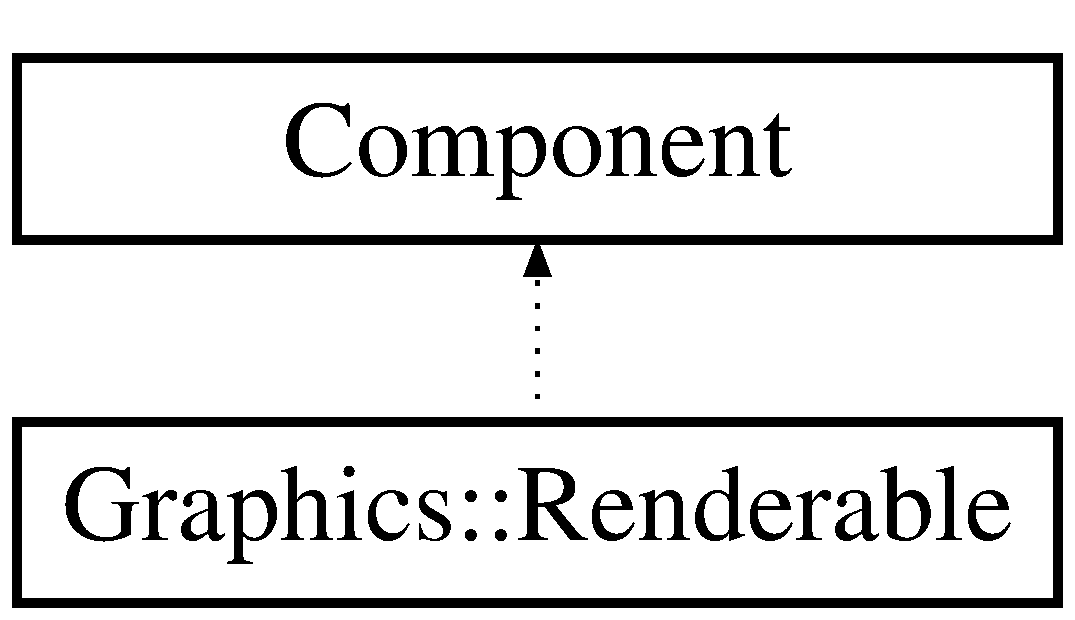
\includegraphics[height=4.000000cm]{class_component}
\end{center}
\end{figure}
\subsection*{Public Member Functions}
\begin{DoxyCompactItemize}
\item 
\hyperlink{class_component_a8775db6d1a2c1afc2e77cd3c8f39da6f}{Component} ()
\item 
virtual void \hyperlink{class_component_a4a528a8790dbc141ffd0aba638b6dcc4}{on\+Start} ()=0
\item 
virtual const bool \hyperlink{class_component_a8be284fccf4e97cee6705bd2d8f3705e}{on\+Update} (const double delta)=0
\item 
virtual void \hyperlink{class_component_a2b198f27162a6caf63917e304295f892}{on\+Destroy} ()=0
\item 
void \hyperlink{class_component_a8842d3ce36b584a3e7d0cb7734232812}{set\+Transform} (std\+::shared\+\_\+ptr$<$ \hyperlink{class_transform}{Transform} $>$ \hyperlink{class_component_a02b1c70de1d9e2c6499dff349da1b0ff}{transform})
\item 
std\+::shared\+\_\+ptr$<$ \hyperlink{class_transform}{Transform} $>$ \hyperlink{class_component_a94dfec102ece6b669176f0609b0a5497}{get\+Transform} () const noexcept
\item 
virtual \hyperlink{class_component_a2e9aa4348314d981f05f67397ad2f872}{$\sim$\+Component} ()
\end{DoxyCompactItemize}
\subsection*{Protected Attributes}
\begin{DoxyCompactItemize}
\item 
std\+::shared\+\_\+ptr$<$ \hyperlink{class_transform}{Transform} $>$ \hyperlink{class_component_a02b1c70de1d9e2c6499dff349da1b0ff}{transform}
\end{DoxyCompactItemize}


\subsection{Constructor \& Destructor Documentation}
\hypertarget{class_component_a8775db6d1a2c1afc2e77cd3c8f39da6f}{}\index{Component@{Component}!Component@{Component}}
\index{Component@{Component}!Component@{Component}}
\subsubsection[{Component}]{\setlength{\rightskip}{0pt plus 5cm}Component\+::\+Component (
\begin{DoxyParamCaption}
{}
\end{DoxyParamCaption}
)}\label{class_component_a8775db6d1a2c1afc2e77cd3c8f39da6f}
\hypertarget{class_component_a2e9aa4348314d981f05f67397ad2f872}{}\index{Component@{Component}!````~Component@{$\sim$\+Component}}
\index{````~Component@{$\sim$\+Component}!Component@{Component}}
\subsubsection[{$\sim$\+Component}]{\setlength{\rightskip}{0pt plus 5cm}virtual Component\+::$\sim$\+Component (
\begin{DoxyParamCaption}
{}
\end{DoxyParamCaption}
)\hspace{0.3cm}{\ttfamily [inline]}, {\ttfamily [virtual]}}\label{class_component_a2e9aa4348314d981f05f67397ad2f872}


\subsection{Member Function Documentation}
\hypertarget{class_component_a94dfec102ece6b669176f0609b0a5497}{}\index{Component@{Component}!get\+Transform@{get\+Transform}}
\index{get\+Transform@{get\+Transform}!Component@{Component}}
\subsubsection[{get\+Transform}]{\setlength{\rightskip}{0pt plus 5cm}std\+::shared\+\_\+ptr$<$ {\bf Transform} $>$ Component\+::get\+Transform (
\begin{DoxyParamCaption}
{}
\end{DoxyParamCaption}
) const\hspace{0.3cm}{\ttfamily [noexcept]}}\label{class_component_a94dfec102ece6b669176f0609b0a5497}
\hypertarget{class_component_a2b198f27162a6caf63917e304295f892}{}\index{Component@{Component}!on\+Destroy@{on\+Destroy}}
\index{on\+Destroy@{on\+Destroy}!Component@{Component}}
\subsubsection[{on\+Destroy}]{\setlength{\rightskip}{0pt plus 5cm}virtual void Component\+::on\+Destroy (
\begin{DoxyParamCaption}
{}
\end{DoxyParamCaption}
)\hspace{0.3cm}{\ttfamily [pure virtual]}}\label{class_component_a2b198f27162a6caf63917e304295f892}


Implemented in \hyperlink{class_graphics_1_1_renderable_a6e20996de55215db7ffae2792aaaa88e}{Graphics\+::\+Renderable}, \hyperlink{class_graphics_1_1_camera_a9d8ca67cbd7a586915fc6cfd303406de}{Graphics\+::\+Camera}, \hyperlink{class_graphics_1_1_light_a7d4ce913fcb79612a90937ae75b3ff2e}{Graphics\+::\+Light}, \hyperlink{class_graphics_1_1_animated_tile_a9781b9b256a666a123fd2c050adb5118}{Graphics\+::\+Animated\+Tile}, and \hyperlink{class_graphics_1_1_tile_a28f5bdfa2fc61b292dda7ec15316b981}{Graphics\+::\+Tile}.

\hypertarget{class_component_a4a528a8790dbc141ffd0aba638b6dcc4}{}\index{Component@{Component}!on\+Start@{on\+Start}}
\index{on\+Start@{on\+Start}!Component@{Component}}
\subsubsection[{on\+Start}]{\setlength{\rightskip}{0pt plus 5cm}virtual void Component\+::on\+Start (
\begin{DoxyParamCaption}
{}
\end{DoxyParamCaption}
)\hspace{0.3cm}{\ttfamily [pure virtual]}}\label{class_component_a4a528a8790dbc141ffd0aba638b6dcc4}


Implemented in \hyperlink{class_graphics_1_1_renderable_a7433551970cd25e0241a4a5bb756ba50}{Graphics\+::\+Renderable}, \hyperlink{class_graphics_1_1_camera_a37edadff497ff3966c2190b876bfe236}{Graphics\+::\+Camera}, \hyperlink{class_graphics_1_1_light_aa8ff320220d375edddae38daec0b3672}{Graphics\+::\+Light}, and \hyperlink{class_graphics_1_1_animated_tile_ad82e39321244cc2e06ee3df527473aba}{Graphics\+::\+Animated\+Tile}.

\hypertarget{class_component_a8be284fccf4e97cee6705bd2d8f3705e}{}\index{Component@{Component}!on\+Update@{on\+Update}}
\index{on\+Update@{on\+Update}!Component@{Component}}
\subsubsection[{on\+Update}]{\setlength{\rightskip}{0pt plus 5cm}virtual const bool Component\+::on\+Update (
\begin{DoxyParamCaption}
\item[{const double}]{delta}
\end{DoxyParamCaption}
)\hspace{0.3cm}{\ttfamily [pure virtual]}}\label{class_component_a8be284fccf4e97cee6705bd2d8f3705e}


Implemented in \hyperlink{class_graphics_1_1_renderable_a7d0e820c55cb7f5c552aa0c1e846db76}{Graphics\+::\+Renderable}, \hyperlink{class_graphics_1_1_camera_a0bfccb5623342c93f69b408937b87374}{Graphics\+::\+Camera}, \hyperlink{class_graphics_1_1_light_ab208fc670894a75038b0e74a75816b21}{Graphics\+::\+Light}, \hyperlink{class_graphics_1_1_animated_tile_a2c6f7cd3866cad84b73ea5da8b92b76e}{Graphics\+::\+Animated\+Tile}, and \hyperlink{class_graphics_1_1_tile_a0311b1d9548f6badc9e81820b110cbb4}{Graphics\+::\+Tile}.

\hypertarget{class_component_a8842d3ce36b584a3e7d0cb7734232812}{}\index{Component@{Component}!set\+Transform@{set\+Transform}}
\index{set\+Transform@{set\+Transform}!Component@{Component}}
\subsubsection[{set\+Transform}]{\setlength{\rightskip}{0pt plus 5cm}void Component\+::set\+Transform (
\begin{DoxyParamCaption}
\item[{std\+::shared\+\_\+ptr$<$ {\bf Transform} $>$}]{transform}
\end{DoxyParamCaption}
)}\label{class_component_a8842d3ce36b584a3e7d0cb7734232812}


\subsection{Member Data Documentation}
\hypertarget{class_component_a02b1c70de1d9e2c6499dff349da1b0ff}{}\index{Component@{Component}!transform@{transform}}
\index{transform@{transform}!Component@{Component}}
\subsubsection[{transform}]{\setlength{\rightskip}{0pt plus 5cm}std\+::shared\+\_\+ptr$<${\bf Transform}$>$ Component\+::transform\hspace{0.3cm}{\ttfamily [protected]}}\label{class_component_a02b1c70de1d9e2c6499dff349da1b0ff}


The documentation for this class was generated from the following files\+:\begin{DoxyCompactItemize}
\item 
src/\hyperlink{component_8h}{component.\+h}\item 
src/\hyperlink{component_8cpp}{component.\+cpp}\end{DoxyCompactItemize}

\hypertarget{class_graphics_1_1_graphics_system}{}\section{Graphics\+:\+:Graphics\+System Class Reference}
\label{class_graphics_1_1_graphics_system}\index{Graphics\+::\+Graphics\+System@{Graphics\+::\+Graphics\+System}}


{\ttfamily \#include $<$graphics\+\_\+system.\+h$>$}

\subsection*{Public Member Functions}
\begin{DoxyCompactItemize}
\item 
\hyperlink{class_graphics_1_1_graphics_system_a748459586ae5ea2aa8721dddb8660de6}{Graphics\+System} ()
\item 
\hyperlink{class_graphics_1_1_graphics_system_a6504df337bfae3a08abc8a63deb6df37}{$\sim$\+Graphics\+System} ()
\item 
void \hyperlink{class_graphics_1_1_graphics_system_a0666cab04b1c7f3ca4dac67f7529cace}{initialize} (const int width, const int height, std\+::string name, const \hyperlink{class_graphics_1_1_window_exit_functor}{Window\+Exit\+Functor} \&\hyperlink{class_graphics_1_1_graphics_system_ac31d552052e7afd10043456ee9393e1a}{window\+\_\+exit}, const double \hyperlink{class_graphics_1_1_graphics_system_ad963821cfb09e6a0e672cf6876e944dd}{max\+\_\+fps}=0.\+0)
\begin{DoxyCompactList}\small\item\em Initializes the graphics system. \end{DoxyCompactList}\item 
const bool \hyperlink{class_graphics_1_1_graphics_system_a1bd027633e66df5a65f2df33952d1dbd}{is\+Initialized} () const noexcept
\begin{DoxyCompactList}\small\item\em Getter to see if system is initialized. \end{DoxyCompactList}\item 
void \hyperlink{class_graphics_1_1_graphics_system_af222ab3a8a83796ad1c12ccf95a6f37a}{render\+Loop} ()
\item 
const int \hyperlink{class_graphics_1_1_graphics_system_a09710fc777ac4db1b44c63c2921d217f}{window\+Height} ()
\begin{DoxyCompactList}\small\item\em Getter for the window width. \end{DoxyCompactList}\item 
const int \hyperlink{class_graphics_1_1_graphics_system_adab3606d554a85ca13aaaec29ceee68c}{window\+Width} ()
\begin{DoxyCompactList}\small\item\em Getter for the window height. \end{DoxyCompactList}\item 
const std\+::string \hyperlink{class_graphics_1_1_graphics_system_a691efb4de942f8da79ecbcf626280724}{window\+Name} () const noexcept
\begin{DoxyCompactList}\small\item\em Getter for the window name. \end{DoxyCompactList}\item 
const int \hyperlink{class_graphics_1_1_graphics_system_ac35c2d3d32e1264b8daad6d59c3aba57}{add\+Renderable} (std\+::shared\+\_\+ptr$<$ \hyperlink{class_graphics_1_1_renderable}{Graphics\+::\+Renderable} $>$ renderable)
\begin{DoxyCompactList}\small\item\em Adds a renderable to the renderable pool. \end{DoxyCompactList}\item 
const bool \hyperlink{class_graphics_1_1_graphics_system_a476b0e6945c37c7b2d48bddcf246a389}{remove\+Renderable} (const int id)
\begin{DoxyCompactList}\small\item\em Removes a renderable from the renderable pool. \end{DoxyCompactList}\item 
const int \hyperlink{class_graphics_1_1_graphics_system_a2b37c3e6f53707002c72c38062be6617}{renderables\+Count} ()
\begin{DoxyCompactList}\small\item\em Returns the number of renderables currently in the system. \end{DoxyCompactList}\item 
const double \hyperlink{class_graphics_1_1_graphics_system_a3266a6af7dd48b4e0501953a5a92d9ee}{get\+Max\+F\+P\+S} () const noexcept
\begin{DoxyCompactList}\small\item\em Returns the max F\+P\+S set on the graphics system. \end{DoxyCompactList}\item 
const double \hyperlink{class_graphics_1_1_graphics_system_a155246106fb6bf556caab7ff9e826524}{get\+Current\+F\+P\+S} () const noexcept
\begin{DoxyCompactList}\small\item\em Returns the current running F\+P\+S on the graphics system. \end{DoxyCompactList}\item 
G\+L\+F\+Wwindow $\ast$ \hyperlink{class_graphics_1_1_graphics_system_a0692ae8d8615f820ed36615e9619fe68}{get\+Current\+Window} () noexcept
\item 
void \hyperlink{class_graphics_1_1_graphics_system_a629d2fe80f761f4f4004ba74ad458e3f}{destroy} ()
\begin{DoxyCompactList}\small\item\em Closes window, and destroys G\+L\+F\+W context. \end{DoxyCompactList}\end{DoxyCompactItemize}
\subsection*{Static Private Member Functions}
\begin{DoxyCompactItemize}
\item 
static void \hyperlink{class_graphics_1_1_graphics_system_a0e3ea1d3785e868d7a1318b4c9c15878}{error\+Callback} (int error, const char $\ast$description)
\end{DoxyCompactItemize}
\subsection*{Private Attributes}
\begin{DoxyCompactItemize}
\item 
G\+L\+F\+Wwindow $\ast$ \hyperlink{class_graphics_1_1_graphics_system_a4430d61bb3fd528b617e8fea26744a8c}{window}
\item 
bool \hyperlink{class_graphics_1_1_graphics_system_a7228e859a8b7da7d9cbc3e151ab2df72}{initialized}
\item 
std\+::string \hyperlink{class_graphics_1_1_graphics_system_a7b543ac0f4323ec286519a3dfef0df1c}{window\+\_\+title}
\item 
std\+::map$<$ int, std\+::shared\+\_\+ptr$<$ \hyperlink{class_graphics_1_1_renderable}{Graphics\+::\+Renderable} $>$ $>$ \hyperlink{class_graphics_1_1_graphics_system_a5dab770243e04860495f894184ef63bb}{renderables\+\_\+map}
\item 
std\+::mutex \hyperlink{class_graphics_1_1_graphics_system_a2e9549405884607a5922a7023a1d2b38}{renderables\+\_\+mutex}
\item 
int \hyperlink{class_graphics_1_1_graphics_system_a950f878ddd2ca0b13a715f4300447903}{next\+\_\+id}
\item 
double \hyperlink{class_graphics_1_1_graphics_system_ad963821cfb09e6a0e672cf6876e944dd}{max\+\_\+fps}
\item 
std\+::atomic$<$ double $>$ \hyperlink{class_graphics_1_1_graphics_system_aa46f6a4cdcae7ff4603c11a650b2986d}{current\+\_\+fps}
\item 
\hyperlink{class_graphics_1_1_window_exit_functor}{Window\+Exit\+Functor} \hyperlink{class_graphics_1_1_graphics_system_ac31d552052e7afd10043456ee9393e1a}{window\+\_\+exit}
\end{DoxyCompactItemize}


\subsection{Constructor \& Destructor Documentation}
\hypertarget{class_graphics_1_1_graphics_system_a748459586ae5ea2aa8721dddb8660de6}{}\index{Graphics\+::\+Graphics\+System@{Graphics\+::\+Graphics\+System}!Graphics\+System@{Graphics\+System}}
\index{Graphics\+System@{Graphics\+System}!Graphics\+::\+Graphics\+System@{Graphics\+::\+Graphics\+System}}
\subsubsection[{Graphics\+System}]{\setlength{\rightskip}{0pt plus 5cm}Graphics\+::\+Graphics\+System\+::\+Graphics\+System (
\begin{DoxyParamCaption}
{}
\end{DoxyParamCaption}
)}\label{class_graphics_1_1_graphics_system_a748459586ae5ea2aa8721dddb8660de6}
\hypertarget{class_graphics_1_1_graphics_system_a6504df337bfae3a08abc8a63deb6df37}{}\index{Graphics\+::\+Graphics\+System@{Graphics\+::\+Graphics\+System}!````~Graphics\+System@{$\sim$\+Graphics\+System}}
\index{````~Graphics\+System@{$\sim$\+Graphics\+System}!Graphics\+::\+Graphics\+System@{Graphics\+::\+Graphics\+System}}
\subsubsection[{$\sim$\+Graphics\+System}]{\setlength{\rightskip}{0pt plus 5cm}Graphics\+::\+Graphics\+System\+::$\sim$\+Graphics\+System (
\begin{DoxyParamCaption}
{}
\end{DoxyParamCaption}
)}\label{class_graphics_1_1_graphics_system_a6504df337bfae3a08abc8a63deb6df37}


\subsection{Member Function Documentation}
\hypertarget{class_graphics_1_1_graphics_system_ac35c2d3d32e1264b8daad6d59c3aba57}{}\index{Graphics\+::\+Graphics\+System@{Graphics\+::\+Graphics\+System}!add\+Renderable@{add\+Renderable}}
\index{add\+Renderable@{add\+Renderable}!Graphics\+::\+Graphics\+System@{Graphics\+::\+Graphics\+System}}
\subsubsection[{add\+Renderable}]{\setlength{\rightskip}{0pt plus 5cm}const int Graphics\+::\+Graphics\+System\+::add\+Renderable (
\begin{DoxyParamCaption}
\item[{std\+::shared\+\_\+ptr$<$ {\bf Graphics\+::\+Renderable} $>$}]{renderable}
\end{DoxyParamCaption}
)}\label{class_graphics_1_1_graphics_system_ac35c2d3d32e1264b8daad6d59c3aba57}


Adds a renderable to the renderable pool. 

Added to the pool of renderables that can be rendered during the update loop.


\begin{DoxyParams}{Parameters}
{\em renderable} & Shared Pointer to a previously created renderable \\
\hline
\end{DoxyParams}
\begin{DoxyReturn}{Returns}
id integer of the renderable 
\end{DoxyReturn}
\hypertarget{class_graphics_1_1_graphics_system_a629d2fe80f761f4f4004ba74ad458e3f}{}\index{Graphics\+::\+Graphics\+System@{Graphics\+::\+Graphics\+System}!destroy@{destroy}}
\index{destroy@{destroy}!Graphics\+::\+Graphics\+System@{Graphics\+::\+Graphics\+System}}
\subsubsection[{destroy}]{\setlength{\rightskip}{0pt plus 5cm}void Graphics\+::\+Graphics\+System\+::destroy (
\begin{DoxyParamCaption}
{}
\end{DoxyParamCaption}
)}\label{class_graphics_1_1_graphics_system_a629d2fe80f761f4f4004ba74ad458e3f}


Closes window, and destroys G\+L\+F\+W context. 

This closes the window created by G\+L\+F\+W and terminates glfw. Initialize must be called to get another window. \hypertarget{class_graphics_1_1_graphics_system_a0e3ea1d3785e868d7a1318b4c9c15878}{}\index{Graphics\+::\+Graphics\+System@{Graphics\+::\+Graphics\+System}!error\+Callback@{error\+Callback}}
\index{error\+Callback@{error\+Callback}!Graphics\+::\+Graphics\+System@{Graphics\+::\+Graphics\+System}}
\subsubsection[{error\+Callback}]{\setlength{\rightskip}{0pt plus 5cm}void Graphics\+::\+Graphics\+System\+::error\+Callback (
\begin{DoxyParamCaption}
\item[{int}]{error, }
\item[{const char $\ast$}]{description}
\end{DoxyParamCaption}
)\hspace{0.3cm}{\ttfamily [static]}, {\ttfamily [private]}}\label{class_graphics_1_1_graphics_system_a0e3ea1d3785e868d7a1318b4c9c15878}
\hypertarget{class_graphics_1_1_graphics_system_a155246106fb6bf556caab7ff9e826524}{}\index{Graphics\+::\+Graphics\+System@{Graphics\+::\+Graphics\+System}!get\+Current\+F\+P\+S@{get\+Current\+F\+P\+S}}
\index{get\+Current\+F\+P\+S@{get\+Current\+F\+P\+S}!Graphics\+::\+Graphics\+System@{Graphics\+::\+Graphics\+System}}
\subsubsection[{get\+Current\+F\+P\+S}]{\setlength{\rightskip}{0pt plus 5cm}const double Graphics\+::\+Graphics\+System\+::get\+Current\+F\+P\+S (
\begin{DoxyParamCaption}
{}
\end{DoxyParamCaption}
) const\hspace{0.3cm}{\ttfamily [noexcept]}}\label{class_graphics_1_1_graphics_system_a155246106fb6bf556caab7ff9e826524}


Returns the current running F\+P\+S on the graphics system. 

This is the current fps that has been recorded as the graphics system is running. \begin{DoxyReturn}{Returns}
double containing the current fps 
\end{DoxyReturn}
\hypertarget{class_graphics_1_1_graphics_system_a0692ae8d8615f820ed36615e9619fe68}{}\index{Graphics\+::\+Graphics\+System@{Graphics\+::\+Graphics\+System}!get\+Current\+Window@{get\+Current\+Window}}
\index{get\+Current\+Window@{get\+Current\+Window}!Graphics\+::\+Graphics\+System@{Graphics\+::\+Graphics\+System}}
\subsubsection[{get\+Current\+Window}]{\setlength{\rightskip}{0pt plus 5cm}G\+L\+F\+Wwindow $\ast$ Graphics\+::\+Graphics\+System\+::get\+Current\+Window (
\begin{DoxyParamCaption}
{}
\end{DoxyParamCaption}
)\hspace{0.3cm}{\ttfamily [noexcept]}}\label{class_graphics_1_1_graphics_system_a0692ae8d8615f820ed36615e9619fe68}
\hypertarget{class_graphics_1_1_graphics_system_a3266a6af7dd48b4e0501953a5a92d9ee}{}\index{Graphics\+::\+Graphics\+System@{Graphics\+::\+Graphics\+System}!get\+Max\+F\+P\+S@{get\+Max\+F\+P\+S}}
\index{get\+Max\+F\+P\+S@{get\+Max\+F\+P\+S}!Graphics\+::\+Graphics\+System@{Graphics\+::\+Graphics\+System}}
\subsubsection[{get\+Max\+F\+P\+S}]{\setlength{\rightskip}{0pt plus 5cm}const double Graphics\+::\+Graphics\+System\+::get\+Max\+F\+P\+S (
\begin{DoxyParamCaption}
{}
\end{DoxyParamCaption}
) const\hspace{0.3cm}{\ttfamily [noexcept]}}\label{class_graphics_1_1_graphics_system_a3266a6af7dd48b4e0501953a5a92d9ee}


Returns the max F\+P\+S set on the graphics system. 

This is the highest frames per second the graphics system can run at (to allow things like vsync) \begin{DoxyReturn}{Returns}
double containing the max fps 
\end{DoxyReturn}
\hypertarget{class_graphics_1_1_graphics_system_a0666cab04b1c7f3ca4dac67f7529cace}{}\index{Graphics\+::\+Graphics\+System@{Graphics\+::\+Graphics\+System}!initialize@{initialize}}
\index{initialize@{initialize}!Graphics\+::\+Graphics\+System@{Graphics\+::\+Graphics\+System}}
\subsubsection[{initialize}]{\setlength{\rightskip}{0pt plus 5cm}void Graphics\+::\+Graphics\+System\+::initialize (
\begin{DoxyParamCaption}
\item[{const int}]{width, }
\item[{const int}]{height, }
\item[{std\+::string}]{name, }
\item[{const {\bf Window\+Exit\+Functor} \&}]{window\+\_\+exit, }
\item[{const double}]{max\+\_\+fps = {\ttfamily 0.0}}
\end{DoxyParamCaption}
)}\label{class_graphics_1_1_graphics_system_a0666cab04b1c7f3ca4dac67f7529cace}


Initializes the graphics system. 

This function initializes the graphics system by creating a G\+L\+F\+W based window at the specified size, and having the supplied name as the window title. Max F\+P\+S can also be supplied to allow V\+S\+Y\+N\+C.


\begin{DoxyParams}{Parameters}
{\em width} & window width in px \\
\hline
{\em height} & window height in px \\
\hline
{\em name} & string containing the name of the window to be built \\
\hline
{\em max\+\_\+fps} & double containing the max allowed fps. Default 0.\+0. \\
\hline
\end{DoxyParams}
\hypertarget{class_graphics_1_1_graphics_system_a1bd027633e66df5a65f2df33952d1dbd}{}\index{Graphics\+::\+Graphics\+System@{Graphics\+::\+Graphics\+System}!is\+Initialized@{is\+Initialized}}
\index{is\+Initialized@{is\+Initialized}!Graphics\+::\+Graphics\+System@{Graphics\+::\+Graphics\+System}}
\subsubsection[{is\+Initialized}]{\setlength{\rightskip}{0pt plus 5cm}const bool Graphics\+::\+Graphics\+System\+::is\+Initialized (
\begin{DoxyParamCaption}
{}
\end{DoxyParamCaption}
) const\hspace{0.3cm}{\ttfamily [noexcept]}}\label{class_graphics_1_1_graphics_system_a1bd027633e66df5a65f2df33952d1dbd}


Getter to see if system is initialized. 

Will return true after \hyperlink{class_graphics_1_1_graphics_system_a0666cab04b1c7f3ca4dac67f7529cace}{initialize()} is called. \begin{DoxyReturn}{Returns}
true if \hyperlink{class_graphics_1_1_graphics_system_a7228e859a8b7da7d9cbc3e151ab2df72}{initialized()} has been called, false otherwise 
\end{DoxyReturn}
\hypertarget{class_graphics_1_1_graphics_system_a476b0e6945c37c7b2d48bddcf246a389}{}\index{Graphics\+::\+Graphics\+System@{Graphics\+::\+Graphics\+System}!remove\+Renderable@{remove\+Renderable}}
\index{remove\+Renderable@{remove\+Renderable}!Graphics\+::\+Graphics\+System@{Graphics\+::\+Graphics\+System}}
\subsubsection[{remove\+Renderable}]{\setlength{\rightskip}{0pt plus 5cm}const bool Graphics\+::\+Graphics\+System\+::remove\+Renderable (
\begin{DoxyParamCaption}
\item[{const int}]{id}
\end{DoxyParamCaption}
)}\label{class_graphics_1_1_graphics_system_a476b0e6945c37c7b2d48bddcf246a389}


Removes a renderable from the renderable pool. 

Removed from the pool of renderables to take it out of the update loop.


\begin{DoxyParams}{Parameters}
{\em id} & id integer of renderable to remove \\
\hline
\end{DoxyParams}
\begin{DoxyReturn}{Returns}
true if successful, false if it didn\textquotesingle{}t exist 
\end{DoxyReturn}
\hypertarget{class_graphics_1_1_graphics_system_a2b37c3e6f53707002c72c38062be6617}{}\index{Graphics\+::\+Graphics\+System@{Graphics\+::\+Graphics\+System}!renderables\+Count@{renderables\+Count}}
\index{renderables\+Count@{renderables\+Count}!Graphics\+::\+Graphics\+System@{Graphics\+::\+Graphics\+System}}
\subsubsection[{renderables\+Count}]{\setlength{\rightskip}{0pt plus 5cm}const int Graphics\+::\+Graphics\+System\+::renderables\+Count (
\begin{DoxyParamCaption}
{}
\end{DoxyParamCaption}
)}\label{class_graphics_1_1_graphics_system_a2b37c3e6f53707002c72c38062be6617}


Returns the number of renderables currently in the system. 

This returns the number of renderables that have been added to the system, and are ready to be updated and rendered. \begin{DoxyReturn}{Returns}
integer representing number of renderables in the system 
\end{DoxyReturn}
\hypertarget{class_graphics_1_1_graphics_system_af222ab3a8a83796ad1c12ccf95a6f37a}{}\index{Graphics\+::\+Graphics\+System@{Graphics\+::\+Graphics\+System}!render\+Loop@{render\+Loop}}
\index{render\+Loop@{render\+Loop}!Graphics\+::\+Graphics\+System@{Graphics\+::\+Graphics\+System}}
\subsubsection[{render\+Loop}]{\setlength{\rightskip}{0pt plus 5cm}void Graphics\+::\+Graphics\+System\+::render\+Loop (
\begin{DoxyParamCaption}
{}
\end{DoxyParamCaption}
)}\label{class_graphics_1_1_graphics_system_af222ab3a8a83796ad1c12ccf95a6f37a}
\hypertarget{class_graphics_1_1_graphics_system_a09710fc777ac4db1b44c63c2921d217f}{}\index{Graphics\+::\+Graphics\+System@{Graphics\+::\+Graphics\+System}!window\+Height@{window\+Height}}
\index{window\+Height@{window\+Height}!Graphics\+::\+Graphics\+System@{Graphics\+::\+Graphics\+System}}
\subsubsection[{window\+Height}]{\setlength{\rightskip}{0pt plus 5cm}const int Graphics\+::\+Graphics\+System\+::window\+Height (
\begin{DoxyParamCaption}
{}
\end{DoxyParamCaption}
)}\label{class_graphics_1_1_graphics_system_a09710fc777ac4db1b44c63c2921d217f}


Getter for the window width. 

This Pings G\+L\+F\+W to get the width of the window. \begin{DoxyReturn}{Returns}
integer denoting pixel width of window 
\end{DoxyReturn}
\hypertarget{class_graphics_1_1_graphics_system_a691efb4de942f8da79ecbcf626280724}{}\index{Graphics\+::\+Graphics\+System@{Graphics\+::\+Graphics\+System}!window\+Name@{window\+Name}}
\index{window\+Name@{window\+Name}!Graphics\+::\+Graphics\+System@{Graphics\+::\+Graphics\+System}}
\subsubsection[{window\+Name}]{\setlength{\rightskip}{0pt plus 5cm}const std\+::string Graphics\+::\+Graphics\+System\+::window\+Name (
\begin{DoxyParamCaption}
{}
\end{DoxyParamCaption}
) const\hspace{0.3cm}{\ttfamily [noexcept]}}\label{class_graphics_1_1_graphics_system_a691efb4de942f8da79ecbcf626280724}


Getter for the window name. 

This will return the name of the window \begin{DoxyReturn}{Returns}
a string that is the name of the window 
\end{DoxyReturn}
\hypertarget{class_graphics_1_1_graphics_system_adab3606d554a85ca13aaaec29ceee68c}{}\index{Graphics\+::\+Graphics\+System@{Graphics\+::\+Graphics\+System}!window\+Width@{window\+Width}}
\index{window\+Width@{window\+Width}!Graphics\+::\+Graphics\+System@{Graphics\+::\+Graphics\+System}}
\subsubsection[{window\+Width}]{\setlength{\rightskip}{0pt plus 5cm}const int Graphics\+::\+Graphics\+System\+::window\+Width (
\begin{DoxyParamCaption}
{}
\end{DoxyParamCaption}
)}\label{class_graphics_1_1_graphics_system_adab3606d554a85ca13aaaec29ceee68c}


Getter for the window height. 

This Pings G\+L\+F\+W to get the height of the window. \begin{DoxyReturn}{Returns}
integer denoting pixel height of window 
\end{DoxyReturn}


\subsection{Member Data Documentation}
\hypertarget{class_graphics_1_1_graphics_system_aa46f6a4cdcae7ff4603c11a650b2986d}{}\index{Graphics\+::\+Graphics\+System@{Graphics\+::\+Graphics\+System}!current\+\_\+fps@{current\+\_\+fps}}
\index{current\+\_\+fps@{current\+\_\+fps}!Graphics\+::\+Graphics\+System@{Graphics\+::\+Graphics\+System}}
\subsubsection[{current\+\_\+fps}]{\setlength{\rightskip}{0pt plus 5cm}std\+::atomic$<$double$>$ Graphics\+::\+Graphics\+System\+::current\+\_\+fps\hspace{0.3cm}{\ttfamily [private]}}\label{class_graphics_1_1_graphics_system_aa46f6a4cdcae7ff4603c11a650b2986d}
\hypertarget{class_graphics_1_1_graphics_system_a7228e859a8b7da7d9cbc3e151ab2df72}{}\index{Graphics\+::\+Graphics\+System@{Graphics\+::\+Graphics\+System}!initialized@{initialized}}
\index{initialized@{initialized}!Graphics\+::\+Graphics\+System@{Graphics\+::\+Graphics\+System}}
\subsubsection[{initialized}]{\setlength{\rightskip}{0pt plus 5cm}bool Graphics\+::\+Graphics\+System\+::initialized\hspace{0.3cm}{\ttfamily [private]}}\label{class_graphics_1_1_graphics_system_a7228e859a8b7da7d9cbc3e151ab2df72}
\hypertarget{class_graphics_1_1_graphics_system_ad963821cfb09e6a0e672cf6876e944dd}{}\index{Graphics\+::\+Graphics\+System@{Graphics\+::\+Graphics\+System}!max\+\_\+fps@{max\+\_\+fps}}
\index{max\+\_\+fps@{max\+\_\+fps}!Graphics\+::\+Graphics\+System@{Graphics\+::\+Graphics\+System}}
\subsubsection[{max\+\_\+fps}]{\setlength{\rightskip}{0pt plus 5cm}double Graphics\+::\+Graphics\+System\+::max\+\_\+fps\hspace{0.3cm}{\ttfamily [private]}}\label{class_graphics_1_1_graphics_system_ad963821cfb09e6a0e672cf6876e944dd}
\hypertarget{class_graphics_1_1_graphics_system_a950f878ddd2ca0b13a715f4300447903}{}\index{Graphics\+::\+Graphics\+System@{Graphics\+::\+Graphics\+System}!next\+\_\+id@{next\+\_\+id}}
\index{next\+\_\+id@{next\+\_\+id}!Graphics\+::\+Graphics\+System@{Graphics\+::\+Graphics\+System}}
\subsubsection[{next\+\_\+id}]{\setlength{\rightskip}{0pt plus 5cm}int Graphics\+::\+Graphics\+System\+::next\+\_\+id\hspace{0.3cm}{\ttfamily [private]}}\label{class_graphics_1_1_graphics_system_a950f878ddd2ca0b13a715f4300447903}
\hypertarget{class_graphics_1_1_graphics_system_a5dab770243e04860495f894184ef63bb}{}\index{Graphics\+::\+Graphics\+System@{Graphics\+::\+Graphics\+System}!renderables\+\_\+map@{renderables\+\_\+map}}
\index{renderables\+\_\+map@{renderables\+\_\+map}!Graphics\+::\+Graphics\+System@{Graphics\+::\+Graphics\+System}}
\subsubsection[{renderables\+\_\+map}]{\setlength{\rightskip}{0pt plus 5cm}std\+::map$<$int, std\+::shared\+\_\+ptr$<${\bf Graphics\+::\+Renderable}$>$ $>$ Graphics\+::\+Graphics\+System\+::renderables\+\_\+map\hspace{0.3cm}{\ttfamily [private]}}\label{class_graphics_1_1_graphics_system_a5dab770243e04860495f894184ef63bb}
\hypertarget{class_graphics_1_1_graphics_system_a2e9549405884607a5922a7023a1d2b38}{}\index{Graphics\+::\+Graphics\+System@{Graphics\+::\+Graphics\+System}!renderables\+\_\+mutex@{renderables\+\_\+mutex}}
\index{renderables\+\_\+mutex@{renderables\+\_\+mutex}!Graphics\+::\+Graphics\+System@{Graphics\+::\+Graphics\+System}}
\subsubsection[{renderables\+\_\+mutex}]{\setlength{\rightskip}{0pt plus 5cm}std\+::mutex Graphics\+::\+Graphics\+System\+::renderables\+\_\+mutex\hspace{0.3cm}{\ttfamily [private]}}\label{class_graphics_1_1_graphics_system_a2e9549405884607a5922a7023a1d2b38}
\hypertarget{class_graphics_1_1_graphics_system_a4430d61bb3fd528b617e8fea26744a8c}{}\index{Graphics\+::\+Graphics\+System@{Graphics\+::\+Graphics\+System}!window@{window}}
\index{window@{window}!Graphics\+::\+Graphics\+System@{Graphics\+::\+Graphics\+System}}
\subsubsection[{window}]{\setlength{\rightskip}{0pt plus 5cm}G\+L\+F\+Wwindow$\ast$ Graphics\+::\+Graphics\+System\+::window\hspace{0.3cm}{\ttfamily [private]}}\label{class_graphics_1_1_graphics_system_a4430d61bb3fd528b617e8fea26744a8c}
\hypertarget{class_graphics_1_1_graphics_system_ac31d552052e7afd10043456ee9393e1a}{}\index{Graphics\+::\+Graphics\+System@{Graphics\+::\+Graphics\+System}!window\+\_\+exit@{window\+\_\+exit}}
\index{window\+\_\+exit@{window\+\_\+exit}!Graphics\+::\+Graphics\+System@{Graphics\+::\+Graphics\+System}}
\subsubsection[{window\+\_\+exit}]{\setlength{\rightskip}{0pt plus 5cm}{\bf Window\+Exit\+Functor} Graphics\+::\+Graphics\+System\+::window\+\_\+exit\hspace{0.3cm}{\ttfamily [private]}}\label{class_graphics_1_1_graphics_system_ac31d552052e7afd10043456ee9393e1a}
\hypertarget{class_graphics_1_1_graphics_system_a7b543ac0f4323ec286519a3dfef0df1c}{}\index{Graphics\+::\+Graphics\+System@{Graphics\+::\+Graphics\+System}!window\+\_\+title@{window\+\_\+title}}
\index{window\+\_\+title@{window\+\_\+title}!Graphics\+::\+Graphics\+System@{Graphics\+::\+Graphics\+System}}
\subsubsection[{window\+\_\+title}]{\setlength{\rightskip}{0pt plus 5cm}std\+::string Graphics\+::\+Graphics\+System\+::window\+\_\+title\hspace{0.3cm}{\ttfamily [private]}}\label{class_graphics_1_1_graphics_system_a7b543ac0f4323ec286519a3dfef0df1c}


The documentation for this class was generated from the following files\+:\begin{DoxyCompactItemize}
\item 
src/graphics/\hyperlink{graphics__system_8h}{graphics\+\_\+system.\+h}\item 
src/graphics/\hyperlink{graphics__system_8cpp}{graphics\+\_\+system.\+cpp}\end{DoxyCompactItemize}

\hypertarget{class_exceptions_1_1_invalid_filename_exception}{}\section{Exceptions\+:\+:Invalid\+Filename\+Exception Class Reference}
\label{class_exceptions_1_1_invalid_filename_exception}\index{Exceptions\+::\+Invalid\+Filename\+Exception@{Exceptions\+::\+Invalid\+Filename\+Exception}}


{\ttfamily \#include $<$invalid\+\_\+filename\+\_\+exception.\+h$>$}

Inheritance diagram for Exceptions\+:\+:Invalid\+Filename\+Exception\+:\begin{figure}[H]
\begin{center}
\leavevmode
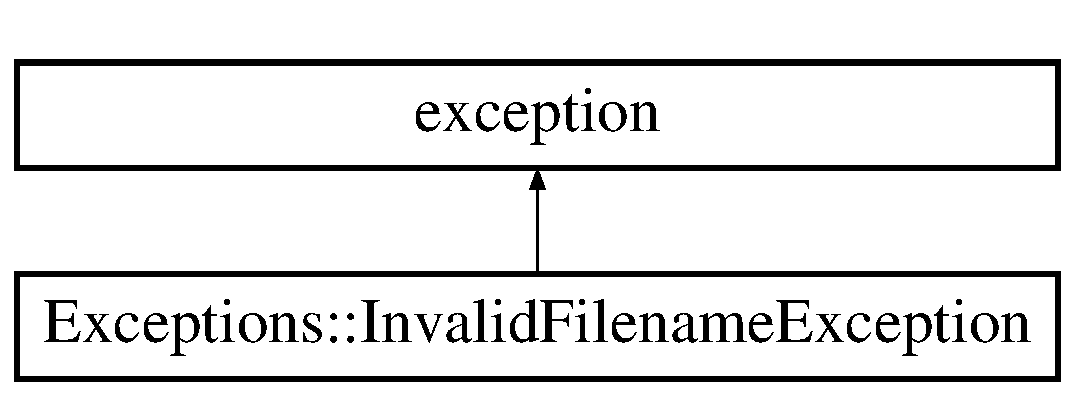
\includegraphics[height=2.000000cm]{class_exceptions_1_1_invalid_filename_exception}
\end{center}
\end{figure}
\subsection*{Public Member Functions}
\begin{DoxyCompactItemize}
\item 
\hyperlink{class_exceptions_1_1_invalid_filename_exception_aa931ab35f59e347af1b19322c02debe3}{Invalid\+Filename\+Exception} (const std\+::string \&\hyperlink{class_exceptions_1_1_invalid_filename_exception_a3c92e5e736e002495079a1537145549e}{filename})
\item 
virtual const char $\ast$ \hyperlink{class_exceptions_1_1_invalid_filename_exception_a4141ce1dc20a4cd02f82ea5a954f716d}{what} () const   throw ()
\end{DoxyCompactItemize}
\subsection*{Private Attributes}
\begin{DoxyCompactItemize}
\item 
std\+::string \hyperlink{class_exceptions_1_1_invalid_filename_exception_a3c92e5e736e002495079a1537145549e}{filename}
\end{DoxyCompactItemize}


\subsection{Constructor \& Destructor Documentation}
\hypertarget{class_exceptions_1_1_invalid_filename_exception_aa931ab35f59e347af1b19322c02debe3}{}\index{Exceptions\+::\+Invalid\+Filename\+Exception@{Exceptions\+::\+Invalid\+Filename\+Exception}!Invalid\+Filename\+Exception@{Invalid\+Filename\+Exception}}
\index{Invalid\+Filename\+Exception@{Invalid\+Filename\+Exception}!Exceptions\+::\+Invalid\+Filename\+Exception@{Exceptions\+::\+Invalid\+Filename\+Exception}}
\subsubsection[{Invalid\+Filename\+Exception}]{\setlength{\rightskip}{0pt plus 5cm}Exceptions\+::\+Invalid\+Filename\+Exception\+::\+Invalid\+Filename\+Exception (
\begin{DoxyParamCaption}
\item[{const std\+::string \&}]{filename}
\end{DoxyParamCaption}
)\hspace{0.3cm}{\ttfamily [inline]}}\label{class_exceptions_1_1_invalid_filename_exception_aa931ab35f59e347af1b19322c02debe3}


\subsection{Member Function Documentation}
\hypertarget{class_exceptions_1_1_invalid_filename_exception_a4141ce1dc20a4cd02f82ea5a954f716d}{}\index{Exceptions\+::\+Invalid\+Filename\+Exception@{Exceptions\+::\+Invalid\+Filename\+Exception}!what@{what}}
\index{what@{what}!Exceptions\+::\+Invalid\+Filename\+Exception@{Exceptions\+::\+Invalid\+Filename\+Exception}}
\subsubsection[{what}]{\setlength{\rightskip}{0pt plus 5cm}virtual const char$\ast$ Exceptions\+::\+Invalid\+Filename\+Exception\+::what (
\begin{DoxyParamCaption}
{}
\end{DoxyParamCaption}
) const throw  ) \hspace{0.3cm}{\ttfamily [inline]}, {\ttfamily [virtual]}}\label{class_exceptions_1_1_invalid_filename_exception_a4141ce1dc20a4cd02f82ea5a954f716d}


\subsection{Member Data Documentation}
\hypertarget{class_exceptions_1_1_invalid_filename_exception_a3c92e5e736e002495079a1537145549e}{}\index{Exceptions\+::\+Invalid\+Filename\+Exception@{Exceptions\+::\+Invalid\+Filename\+Exception}!filename@{filename}}
\index{filename@{filename}!Exceptions\+::\+Invalid\+Filename\+Exception@{Exceptions\+::\+Invalid\+Filename\+Exception}}
\subsubsection[{filename}]{\setlength{\rightskip}{0pt plus 5cm}std\+::string Exceptions\+::\+Invalid\+Filename\+Exception\+::filename\hspace{0.3cm}{\ttfamily [private]}}\label{class_exceptions_1_1_invalid_filename_exception_a3c92e5e736e002495079a1537145549e}


The documentation for this class was generated from the following file\+:\begin{DoxyCompactItemize}
\item 
src/exceptions/\hyperlink{invalid__filename__exception_8h}{invalid\+\_\+filename\+\_\+exception.\+h}\end{DoxyCompactItemize}

\hypertarget{class_exceptions_1_1_invalid_fragment_shader_exception}{}\section{Exceptions\+:\+:Invalid\+Fragment\+Shader\+Exception Class Reference}
\label{class_exceptions_1_1_invalid_fragment_shader_exception}\index{Exceptions\+::\+Invalid\+Fragment\+Shader\+Exception@{Exceptions\+::\+Invalid\+Fragment\+Shader\+Exception}}


{\ttfamily \#include $<$invalid\+\_\+fragment\+\_\+shader\+\_\+exception.\+h$>$}

Inheritance diagram for Exceptions\+:\+:Invalid\+Fragment\+Shader\+Exception\+:\begin{figure}[H]
\begin{center}
\leavevmode
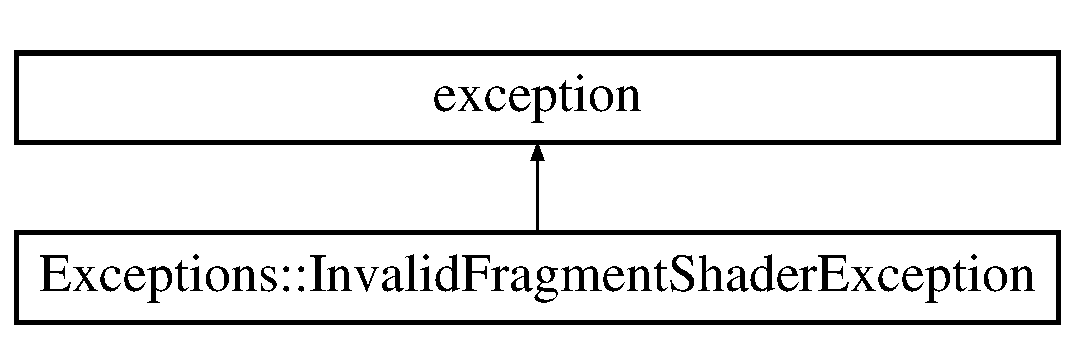
\includegraphics[height=2.000000cm]{class_exceptions_1_1_invalid_fragment_shader_exception}
\end{center}
\end{figure}
\subsection*{Public Member Functions}
\begin{DoxyCompactItemize}
\item 
\hyperlink{class_exceptions_1_1_invalid_fragment_shader_exception_adc23c55b308ae7ef93d03a6eee4bda31}{Invalid\+Fragment\+Shader\+Exception} (const unsigned int \hyperlink{class_exceptions_1_1_invalid_fragment_shader_exception_a3b2f1a947996d185b7a8a5c669ebbc74}{fragment\+\_\+shader\+\_\+binding})
\item 
virtual const char $\ast$ \hyperlink{class_exceptions_1_1_invalid_fragment_shader_exception_a816958e8042838f5a7ea88cefb4ea86c}{what} () const   throw ()
\end{DoxyCompactItemize}
\subsection*{Private Attributes}
\begin{DoxyCompactItemize}
\item 
unsigned int \hyperlink{class_exceptions_1_1_invalid_fragment_shader_exception_a3b2f1a947996d185b7a8a5c669ebbc74}{fragment\+\_\+shader\+\_\+binding}
\end{DoxyCompactItemize}


\subsection{Constructor \& Destructor Documentation}
\hypertarget{class_exceptions_1_1_invalid_fragment_shader_exception_adc23c55b308ae7ef93d03a6eee4bda31}{}\index{Exceptions\+::\+Invalid\+Fragment\+Shader\+Exception@{Exceptions\+::\+Invalid\+Fragment\+Shader\+Exception}!Invalid\+Fragment\+Shader\+Exception@{Invalid\+Fragment\+Shader\+Exception}}
\index{Invalid\+Fragment\+Shader\+Exception@{Invalid\+Fragment\+Shader\+Exception}!Exceptions\+::\+Invalid\+Fragment\+Shader\+Exception@{Exceptions\+::\+Invalid\+Fragment\+Shader\+Exception}}
\subsubsection[{Invalid\+Fragment\+Shader\+Exception}]{\setlength{\rightskip}{0pt plus 5cm}Exceptions\+::\+Invalid\+Fragment\+Shader\+Exception\+::\+Invalid\+Fragment\+Shader\+Exception (
\begin{DoxyParamCaption}
\item[{const unsigned int}]{fragment\+\_\+shader\+\_\+binding}
\end{DoxyParamCaption}
)\hspace{0.3cm}{\ttfamily [inline]}}\label{class_exceptions_1_1_invalid_fragment_shader_exception_adc23c55b308ae7ef93d03a6eee4bda31}


\subsection{Member Function Documentation}
\hypertarget{class_exceptions_1_1_invalid_fragment_shader_exception_a816958e8042838f5a7ea88cefb4ea86c}{}\index{Exceptions\+::\+Invalid\+Fragment\+Shader\+Exception@{Exceptions\+::\+Invalid\+Fragment\+Shader\+Exception}!what@{what}}
\index{what@{what}!Exceptions\+::\+Invalid\+Fragment\+Shader\+Exception@{Exceptions\+::\+Invalid\+Fragment\+Shader\+Exception}}
\subsubsection[{what}]{\setlength{\rightskip}{0pt plus 5cm}virtual const char$\ast$ Exceptions\+::\+Invalid\+Fragment\+Shader\+Exception\+::what (
\begin{DoxyParamCaption}
{}
\end{DoxyParamCaption}
) const throw  ) \hspace{0.3cm}{\ttfamily [inline]}, {\ttfamily [virtual]}}\label{class_exceptions_1_1_invalid_fragment_shader_exception_a816958e8042838f5a7ea88cefb4ea86c}


\subsection{Member Data Documentation}
\hypertarget{class_exceptions_1_1_invalid_fragment_shader_exception_a3b2f1a947996d185b7a8a5c669ebbc74}{}\index{Exceptions\+::\+Invalid\+Fragment\+Shader\+Exception@{Exceptions\+::\+Invalid\+Fragment\+Shader\+Exception}!fragment\+\_\+shader\+\_\+binding@{fragment\+\_\+shader\+\_\+binding}}
\index{fragment\+\_\+shader\+\_\+binding@{fragment\+\_\+shader\+\_\+binding}!Exceptions\+::\+Invalid\+Fragment\+Shader\+Exception@{Exceptions\+::\+Invalid\+Fragment\+Shader\+Exception}}
\subsubsection[{fragment\+\_\+shader\+\_\+binding}]{\setlength{\rightskip}{0pt plus 5cm}unsigned int Exceptions\+::\+Invalid\+Fragment\+Shader\+Exception\+::fragment\+\_\+shader\+\_\+binding\hspace{0.3cm}{\ttfamily [private]}}\label{class_exceptions_1_1_invalid_fragment_shader_exception_a3b2f1a947996d185b7a8a5c669ebbc74}


The documentation for this class was generated from the following file\+:\begin{DoxyCompactItemize}
\item 
src/exceptions/\hyperlink{invalid__fragment__shader__exception_8h}{invalid\+\_\+fragment\+\_\+shader\+\_\+exception.\+h}\end{DoxyCompactItemize}

\hypertarget{class_exceptions_1_1_invalid_geometry_shader_exception}{}\section{Exceptions\+:\+:Invalid\+Geometry\+Shader\+Exception Class Reference}
\label{class_exceptions_1_1_invalid_geometry_shader_exception}\index{Exceptions\+::\+Invalid\+Geometry\+Shader\+Exception@{Exceptions\+::\+Invalid\+Geometry\+Shader\+Exception}}


{\ttfamily \#include $<$invalid\+\_\+geometry\+\_\+shader\+\_\+exception.\+h$>$}

Inheritance diagram for Exceptions\+:\+:Invalid\+Geometry\+Shader\+Exception\+:\begin{figure}[H]
\begin{center}
\leavevmode
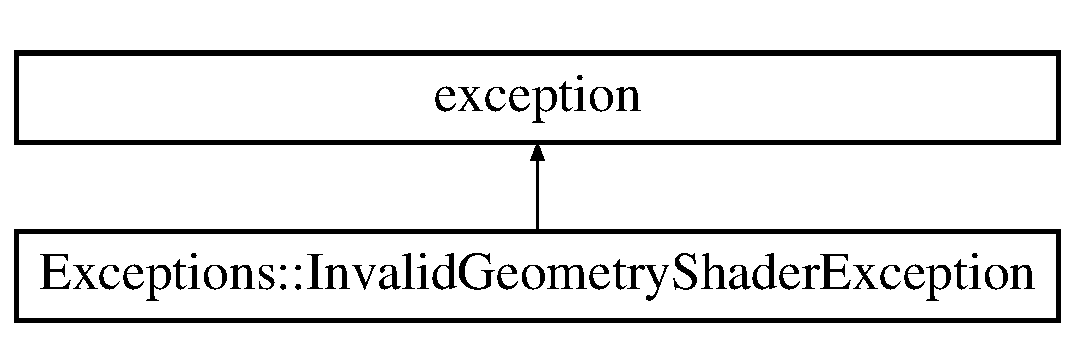
\includegraphics[height=2.000000cm]{class_exceptions_1_1_invalid_geometry_shader_exception}
\end{center}
\end{figure}
\subsection*{Public Member Functions}
\begin{DoxyCompactItemize}
\item 
\hyperlink{class_exceptions_1_1_invalid_geometry_shader_exception_abd1bf3f98bbb1a590d2d67e36b9d4b75}{Invalid\+Geometry\+Shader\+Exception} (const unsigned int \hyperlink{class_exceptions_1_1_invalid_geometry_shader_exception_a9b392c914b5d558b6ef0eaf130eb7ce9}{geometry\+\_\+shader\+\_\+binding})
\item 
virtual const char $\ast$ \hyperlink{class_exceptions_1_1_invalid_geometry_shader_exception_a9661fdb92878acabb635d02584005e81}{what} () const   throw ()
\end{DoxyCompactItemize}
\subsection*{Private Attributes}
\begin{DoxyCompactItemize}
\item 
unsigned int \hyperlink{class_exceptions_1_1_invalid_geometry_shader_exception_a9b392c914b5d558b6ef0eaf130eb7ce9}{geometry\+\_\+shader\+\_\+binding}
\end{DoxyCompactItemize}


\subsection{Constructor \& Destructor Documentation}
\hypertarget{class_exceptions_1_1_invalid_geometry_shader_exception_abd1bf3f98bbb1a590d2d67e36b9d4b75}{}\index{Exceptions\+::\+Invalid\+Geometry\+Shader\+Exception@{Exceptions\+::\+Invalid\+Geometry\+Shader\+Exception}!Invalid\+Geometry\+Shader\+Exception@{Invalid\+Geometry\+Shader\+Exception}}
\index{Invalid\+Geometry\+Shader\+Exception@{Invalid\+Geometry\+Shader\+Exception}!Exceptions\+::\+Invalid\+Geometry\+Shader\+Exception@{Exceptions\+::\+Invalid\+Geometry\+Shader\+Exception}}
\subsubsection[{Invalid\+Geometry\+Shader\+Exception}]{\setlength{\rightskip}{0pt plus 5cm}Exceptions\+::\+Invalid\+Geometry\+Shader\+Exception\+::\+Invalid\+Geometry\+Shader\+Exception (
\begin{DoxyParamCaption}
\item[{const unsigned int}]{geometry\+\_\+shader\+\_\+binding}
\end{DoxyParamCaption}
)\hspace{0.3cm}{\ttfamily [inline]}}\label{class_exceptions_1_1_invalid_geometry_shader_exception_abd1bf3f98bbb1a590d2d67e36b9d4b75}


\subsection{Member Function Documentation}
\hypertarget{class_exceptions_1_1_invalid_geometry_shader_exception_a9661fdb92878acabb635d02584005e81}{}\index{Exceptions\+::\+Invalid\+Geometry\+Shader\+Exception@{Exceptions\+::\+Invalid\+Geometry\+Shader\+Exception}!what@{what}}
\index{what@{what}!Exceptions\+::\+Invalid\+Geometry\+Shader\+Exception@{Exceptions\+::\+Invalid\+Geometry\+Shader\+Exception}}
\subsubsection[{what}]{\setlength{\rightskip}{0pt plus 5cm}virtual const char$\ast$ Exceptions\+::\+Invalid\+Geometry\+Shader\+Exception\+::what (
\begin{DoxyParamCaption}
{}
\end{DoxyParamCaption}
) const throw  ) \hspace{0.3cm}{\ttfamily [inline]}, {\ttfamily [virtual]}}\label{class_exceptions_1_1_invalid_geometry_shader_exception_a9661fdb92878acabb635d02584005e81}


\subsection{Member Data Documentation}
\hypertarget{class_exceptions_1_1_invalid_geometry_shader_exception_a9b392c914b5d558b6ef0eaf130eb7ce9}{}\index{Exceptions\+::\+Invalid\+Geometry\+Shader\+Exception@{Exceptions\+::\+Invalid\+Geometry\+Shader\+Exception}!geometry\+\_\+shader\+\_\+binding@{geometry\+\_\+shader\+\_\+binding}}
\index{geometry\+\_\+shader\+\_\+binding@{geometry\+\_\+shader\+\_\+binding}!Exceptions\+::\+Invalid\+Geometry\+Shader\+Exception@{Exceptions\+::\+Invalid\+Geometry\+Shader\+Exception}}
\subsubsection[{geometry\+\_\+shader\+\_\+binding}]{\setlength{\rightskip}{0pt plus 5cm}unsigned int Exceptions\+::\+Invalid\+Geometry\+Shader\+Exception\+::geometry\+\_\+shader\+\_\+binding\hspace{0.3cm}{\ttfamily [private]}}\label{class_exceptions_1_1_invalid_geometry_shader_exception_a9b392c914b5d558b6ef0eaf130eb7ce9}


The documentation for this class was generated from the following file\+:\begin{DoxyCompactItemize}
\item 
src/exceptions/\hyperlink{invalid__geometry__shader__exception_8h}{invalid\+\_\+geometry\+\_\+shader\+\_\+exception.\+h}\end{DoxyCompactItemize}

\hypertarget{class_exceptions_1_1_invalid_shader_name_exception}{}\section{Exceptions\+:\+:Invalid\+Shader\+Name\+Exception Class Reference}
\label{class_exceptions_1_1_invalid_shader_name_exception}\index{Exceptions\+::\+Invalid\+Shader\+Name\+Exception@{Exceptions\+::\+Invalid\+Shader\+Name\+Exception}}


{\ttfamily \#include $<$invalid\+\_\+shader\+\_\+name\+\_\+exception.\+h$>$}

Inheritance diagram for Exceptions\+:\+:Invalid\+Shader\+Name\+Exception\+:\begin{figure}[H]
\begin{center}
\leavevmode
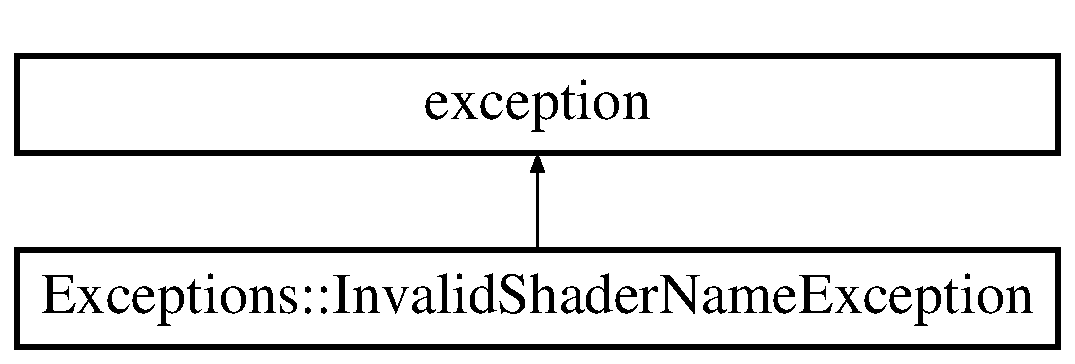
\includegraphics[height=2.000000cm]{class_exceptions_1_1_invalid_shader_name_exception}
\end{center}
\end{figure}
\subsection*{Public Member Functions}
\begin{DoxyCompactItemize}
\item 
\hyperlink{class_exceptions_1_1_invalid_shader_name_exception_a83014c98e72fb045d664a5af323ab023}{Invalid\+Shader\+Name\+Exception} (const std\+::string \&\hyperlink{class_exceptions_1_1_invalid_shader_name_exception_a3d9438219209a9bfe42df58f3107e3c8}{name})
\item 
virtual const char $\ast$ \hyperlink{class_exceptions_1_1_invalid_shader_name_exception_a8a01046b3d3cb4b8459d5f263c2c9295}{what} () const   throw ()
\end{DoxyCompactItemize}
\subsection*{Private Attributes}
\begin{DoxyCompactItemize}
\item 
std\+::string \hyperlink{class_exceptions_1_1_invalid_shader_name_exception_a3d9438219209a9bfe42df58f3107e3c8}{name}
\end{DoxyCompactItemize}


\subsection{Constructor \& Destructor Documentation}
\hypertarget{class_exceptions_1_1_invalid_shader_name_exception_a83014c98e72fb045d664a5af323ab023}{}\index{Exceptions\+::\+Invalid\+Shader\+Name\+Exception@{Exceptions\+::\+Invalid\+Shader\+Name\+Exception}!Invalid\+Shader\+Name\+Exception@{Invalid\+Shader\+Name\+Exception}}
\index{Invalid\+Shader\+Name\+Exception@{Invalid\+Shader\+Name\+Exception}!Exceptions\+::\+Invalid\+Shader\+Name\+Exception@{Exceptions\+::\+Invalid\+Shader\+Name\+Exception}}
\subsubsection[{Invalid\+Shader\+Name\+Exception}]{\setlength{\rightskip}{0pt plus 5cm}Exceptions\+::\+Invalid\+Shader\+Name\+Exception\+::\+Invalid\+Shader\+Name\+Exception (
\begin{DoxyParamCaption}
\item[{const std\+::string \&}]{name}
\end{DoxyParamCaption}
)\hspace{0.3cm}{\ttfamily [inline]}}\label{class_exceptions_1_1_invalid_shader_name_exception_a83014c98e72fb045d664a5af323ab023}


\subsection{Member Function Documentation}
\hypertarget{class_exceptions_1_1_invalid_shader_name_exception_a8a01046b3d3cb4b8459d5f263c2c9295}{}\index{Exceptions\+::\+Invalid\+Shader\+Name\+Exception@{Exceptions\+::\+Invalid\+Shader\+Name\+Exception}!what@{what}}
\index{what@{what}!Exceptions\+::\+Invalid\+Shader\+Name\+Exception@{Exceptions\+::\+Invalid\+Shader\+Name\+Exception}}
\subsubsection[{what}]{\setlength{\rightskip}{0pt plus 5cm}virtual const char$\ast$ Exceptions\+::\+Invalid\+Shader\+Name\+Exception\+::what (
\begin{DoxyParamCaption}
{}
\end{DoxyParamCaption}
) const throw  ) \hspace{0.3cm}{\ttfamily [inline]}, {\ttfamily [virtual]}}\label{class_exceptions_1_1_invalid_shader_name_exception_a8a01046b3d3cb4b8459d5f263c2c9295}


\subsection{Member Data Documentation}
\hypertarget{class_exceptions_1_1_invalid_shader_name_exception_a3d9438219209a9bfe42df58f3107e3c8}{}\index{Exceptions\+::\+Invalid\+Shader\+Name\+Exception@{Exceptions\+::\+Invalid\+Shader\+Name\+Exception}!name@{name}}
\index{name@{name}!Exceptions\+::\+Invalid\+Shader\+Name\+Exception@{Exceptions\+::\+Invalid\+Shader\+Name\+Exception}}
\subsubsection[{name}]{\setlength{\rightskip}{0pt plus 5cm}std\+::string Exceptions\+::\+Invalid\+Shader\+Name\+Exception\+::name\hspace{0.3cm}{\ttfamily [private]}}\label{class_exceptions_1_1_invalid_shader_name_exception_a3d9438219209a9bfe42df58f3107e3c8}


The documentation for this class was generated from the following file\+:\begin{DoxyCompactItemize}
\item 
src/exceptions/\hyperlink{invalid__shader__name__exception_8h}{invalid\+\_\+shader\+\_\+name\+\_\+exception.\+h}\end{DoxyCompactItemize}

\hypertarget{class_exceptions_1_1_invalid_shader_object_exception}{}\section{Exceptions\+:\+:Invalid\+Shader\+Object\+Exception Class Reference}
\label{class_exceptions_1_1_invalid_shader_object_exception}\index{Exceptions\+::\+Invalid\+Shader\+Object\+Exception@{Exceptions\+::\+Invalid\+Shader\+Object\+Exception}}


{\ttfamily \#include $<$invalid\+\_\+shader\+\_\+object\+\_\+exception.\+h$>$}

Inheritance diagram for Exceptions\+:\+:Invalid\+Shader\+Object\+Exception\+:\begin{figure}[H]
\begin{center}
\leavevmode
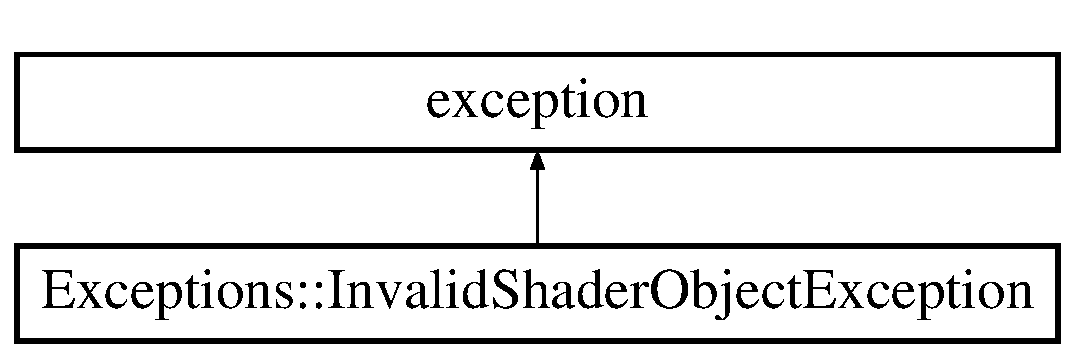
\includegraphics[height=2.000000cm]{class_exceptions_1_1_invalid_shader_object_exception}
\end{center}
\end{figure}
\subsection*{Public Member Functions}
\begin{DoxyCompactItemize}
\item 
\hyperlink{class_exceptions_1_1_invalid_shader_object_exception_a7de090bec61f4d09e95a6286a96e9f25}{Invalid\+Shader\+Object\+Exception} (const unsigned int \hyperlink{class_exceptions_1_1_invalid_shader_object_exception_a80365b85ba22f19254ea8e04cd0454e0}{shader\+\_\+object\+\_\+binding})
\item 
virtual const char $\ast$ \hyperlink{class_exceptions_1_1_invalid_shader_object_exception_a31caa1597313fbe9e166146b266087b0}{what} () const   throw ()
\end{DoxyCompactItemize}
\subsection*{Private Attributes}
\begin{DoxyCompactItemize}
\item 
unsigned int \hyperlink{class_exceptions_1_1_invalid_shader_object_exception_a80365b85ba22f19254ea8e04cd0454e0}{shader\+\_\+object\+\_\+binding}
\end{DoxyCompactItemize}


\subsection{Constructor \& Destructor Documentation}
\hypertarget{class_exceptions_1_1_invalid_shader_object_exception_a7de090bec61f4d09e95a6286a96e9f25}{}\index{Exceptions\+::\+Invalid\+Shader\+Object\+Exception@{Exceptions\+::\+Invalid\+Shader\+Object\+Exception}!Invalid\+Shader\+Object\+Exception@{Invalid\+Shader\+Object\+Exception}}
\index{Invalid\+Shader\+Object\+Exception@{Invalid\+Shader\+Object\+Exception}!Exceptions\+::\+Invalid\+Shader\+Object\+Exception@{Exceptions\+::\+Invalid\+Shader\+Object\+Exception}}
\subsubsection[{Invalid\+Shader\+Object\+Exception}]{\setlength{\rightskip}{0pt plus 5cm}Exceptions\+::\+Invalid\+Shader\+Object\+Exception\+::\+Invalid\+Shader\+Object\+Exception (
\begin{DoxyParamCaption}
\item[{const unsigned int}]{shader\+\_\+object\+\_\+binding}
\end{DoxyParamCaption}
)\hspace{0.3cm}{\ttfamily [inline]}}\label{class_exceptions_1_1_invalid_shader_object_exception_a7de090bec61f4d09e95a6286a96e9f25}


\subsection{Member Function Documentation}
\hypertarget{class_exceptions_1_1_invalid_shader_object_exception_a31caa1597313fbe9e166146b266087b0}{}\index{Exceptions\+::\+Invalid\+Shader\+Object\+Exception@{Exceptions\+::\+Invalid\+Shader\+Object\+Exception}!what@{what}}
\index{what@{what}!Exceptions\+::\+Invalid\+Shader\+Object\+Exception@{Exceptions\+::\+Invalid\+Shader\+Object\+Exception}}
\subsubsection[{what}]{\setlength{\rightskip}{0pt plus 5cm}virtual const char$\ast$ Exceptions\+::\+Invalid\+Shader\+Object\+Exception\+::what (
\begin{DoxyParamCaption}
{}
\end{DoxyParamCaption}
) const throw  ) \hspace{0.3cm}{\ttfamily [inline]}, {\ttfamily [virtual]}}\label{class_exceptions_1_1_invalid_shader_object_exception_a31caa1597313fbe9e166146b266087b0}


\subsection{Member Data Documentation}
\hypertarget{class_exceptions_1_1_invalid_shader_object_exception_a80365b85ba22f19254ea8e04cd0454e0}{}\index{Exceptions\+::\+Invalid\+Shader\+Object\+Exception@{Exceptions\+::\+Invalid\+Shader\+Object\+Exception}!shader\+\_\+object\+\_\+binding@{shader\+\_\+object\+\_\+binding}}
\index{shader\+\_\+object\+\_\+binding@{shader\+\_\+object\+\_\+binding}!Exceptions\+::\+Invalid\+Shader\+Object\+Exception@{Exceptions\+::\+Invalid\+Shader\+Object\+Exception}}
\subsubsection[{shader\+\_\+object\+\_\+binding}]{\setlength{\rightskip}{0pt plus 5cm}unsigned int Exceptions\+::\+Invalid\+Shader\+Object\+Exception\+::shader\+\_\+object\+\_\+binding\hspace{0.3cm}{\ttfamily [private]}}\label{class_exceptions_1_1_invalid_shader_object_exception_a80365b85ba22f19254ea8e04cd0454e0}


The documentation for this class was generated from the following file\+:\begin{DoxyCompactItemize}
\item 
src/exceptions/\hyperlink{invalid__shader__object__exception_8h}{invalid\+\_\+shader\+\_\+object\+\_\+exception.\+h}\end{DoxyCompactItemize}

\hypertarget{class_exceptions_1_1_invalid_shader_program_exception}{}\section{Exceptions\+:\+:Invalid\+Shader\+Program\+Exception Class Reference}
\label{class_exceptions_1_1_invalid_shader_program_exception}\index{Exceptions\+::\+Invalid\+Shader\+Program\+Exception@{Exceptions\+::\+Invalid\+Shader\+Program\+Exception}}


{\ttfamily \#include $<$invalid\+\_\+shader\+\_\+program\+\_\+exception.\+h$>$}

Inheritance diagram for Exceptions\+:\+:Invalid\+Shader\+Program\+Exception\+:\begin{figure}[H]
\begin{center}
\leavevmode
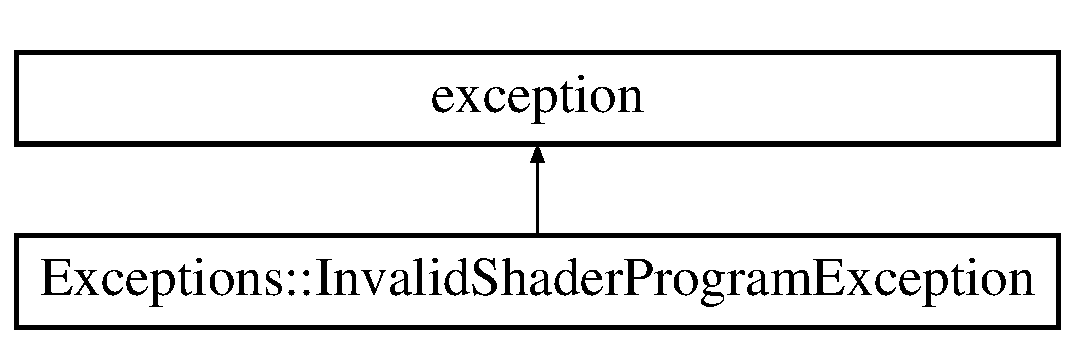
\includegraphics[height=2.000000cm]{class_exceptions_1_1_invalid_shader_program_exception}
\end{center}
\end{figure}
\subsection*{Public Member Functions}
\begin{DoxyCompactItemize}
\item 
\hyperlink{class_exceptions_1_1_invalid_shader_program_exception_aaa3d4fe606a35fd3ae882bf9e00da7c2}{Invalid\+Shader\+Program\+Exception} (const unsigned int \hyperlink{class_exceptions_1_1_invalid_shader_program_exception_ad04a0590a5111a7267ca56dc595efb28}{shader\+\_\+program})
\item 
virtual const char $\ast$ \hyperlink{class_exceptions_1_1_invalid_shader_program_exception_a5fc30a59b16fc5afae6211b289177ce8}{what} () const   throw ()
\end{DoxyCompactItemize}
\subsection*{Private Attributes}
\begin{DoxyCompactItemize}
\item 
unsigned int \hyperlink{class_exceptions_1_1_invalid_shader_program_exception_ad04a0590a5111a7267ca56dc595efb28}{shader\+\_\+program}
\end{DoxyCompactItemize}


\subsection{Constructor \& Destructor Documentation}
\hypertarget{class_exceptions_1_1_invalid_shader_program_exception_aaa3d4fe606a35fd3ae882bf9e00da7c2}{}\index{Exceptions\+::\+Invalid\+Shader\+Program\+Exception@{Exceptions\+::\+Invalid\+Shader\+Program\+Exception}!Invalid\+Shader\+Program\+Exception@{Invalid\+Shader\+Program\+Exception}}
\index{Invalid\+Shader\+Program\+Exception@{Invalid\+Shader\+Program\+Exception}!Exceptions\+::\+Invalid\+Shader\+Program\+Exception@{Exceptions\+::\+Invalid\+Shader\+Program\+Exception}}
\subsubsection[{Invalid\+Shader\+Program\+Exception}]{\setlength{\rightskip}{0pt plus 5cm}Exceptions\+::\+Invalid\+Shader\+Program\+Exception\+::\+Invalid\+Shader\+Program\+Exception (
\begin{DoxyParamCaption}
\item[{const unsigned int}]{shader\+\_\+program}
\end{DoxyParamCaption}
)\hspace{0.3cm}{\ttfamily [inline]}}\label{class_exceptions_1_1_invalid_shader_program_exception_aaa3d4fe606a35fd3ae882bf9e00da7c2}


\subsection{Member Function Documentation}
\hypertarget{class_exceptions_1_1_invalid_shader_program_exception_a5fc30a59b16fc5afae6211b289177ce8}{}\index{Exceptions\+::\+Invalid\+Shader\+Program\+Exception@{Exceptions\+::\+Invalid\+Shader\+Program\+Exception}!what@{what}}
\index{what@{what}!Exceptions\+::\+Invalid\+Shader\+Program\+Exception@{Exceptions\+::\+Invalid\+Shader\+Program\+Exception}}
\subsubsection[{what}]{\setlength{\rightskip}{0pt plus 5cm}virtual const char$\ast$ Exceptions\+::\+Invalid\+Shader\+Program\+Exception\+::what (
\begin{DoxyParamCaption}
{}
\end{DoxyParamCaption}
) const throw  ) \hspace{0.3cm}{\ttfamily [inline]}, {\ttfamily [virtual]}}\label{class_exceptions_1_1_invalid_shader_program_exception_a5fc30a59b16fc5afae6211b289177ce8}


\subsection{Member Data Documentation}
\hypertarget{class_exceptions_1_1_invalid_shader_program_exception_ad04a0590a5111a7267ca56dc595efb28}{}\index{Exceptions\+::\+Invalid\+Shader\+Program\+Exception@{Exceptions\+::\+Invalid\+Shader\+Program\+Exception}!shader\+\_\+program@{shader\+\_\+program}}
\index{shader\+\_\+program@{shader\+\_\+program}!Exceptions\+::\+Invalid\+Shader\+Program\+Exception@{Exceptions\+::\+Invalid\+Shader\+Program\+Exception}}
\subsubsection[{shader\+\_\+program}]{\setlength{\rightskip}{0pt plus 5cm}unsigned int Exceptions\+::\+Invalid\+Shader\+Program\+Exception\+::shader\+\_\+program\hspace{0.3cm}{\ttfamily [private]}}\label{class_exceptions_1_1_invalid_shader_program_exception_ad04a0590a5111a7267ca56dc595efb28}


The documentation for this class was generated from the following file\+:\begin{DoxyCompactItemize}
\item 
src/exceptions/\hyperlink{invalid__shader__program__exception_8h}{invalid\+\_\+shader\+\_\+program\+\_\+exception.\+h}\end{DoxyCompactItemize}

\hypertarget{class_exceptions_1_1_invalid_uniform_name_exception}{}\section{Exceptions\+:\+:Invalid\+Uniform\+Name\+Exception Class Reference}
\label{class_exceptions_1_1_invalid_uniform_name_exception}\index{Exceptions\+::\+Invalid\+Uniform\+Name\+Exception@{Exceptions\+::\+Invalid\+Uniform\+Name\+Exception}}


{\ttfamily \#include $<$invalid\+\_\+uniform\+\_\+name\+\_\+exception.\+h$>$}

Inheritance diagram for Exceptions\+:\+:Invalid\+Uniform\+Name\+Exception\+:\begin{figure}[H]
\begin{center}
\leavevmode
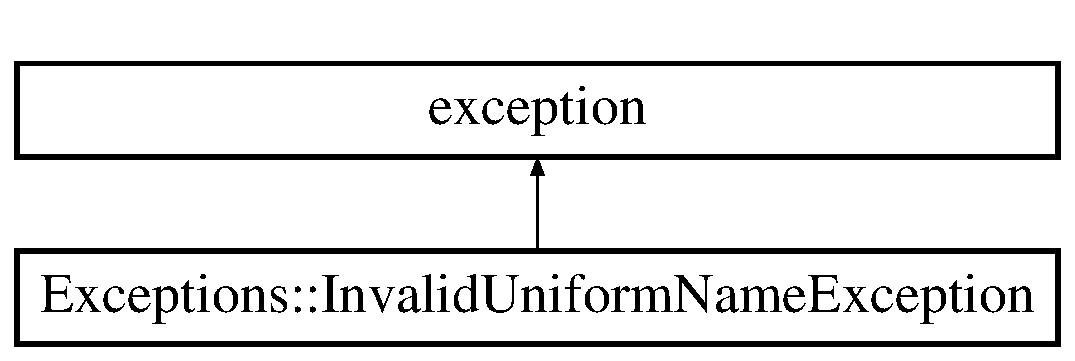
\includegraphics[height=2.000000cm]{class_exceptions_1_1_invalid_uniform_name_exception}
\end{center}
\end{figure}
\subsection*{Public Member Functions}
\begin{DoxyCompactItemize}
\item 
\hyperlink{class_exceptions_1_1_invalid_uniform_name_exception_a1eb355e5fbb46a511d5b94a6918eca31}{Invalid\+Uniform\+Name\+Exception} (const std\+::string \hyperlink{class_exceptions_1_1_invalid_uniform_name_exception_a6cb6b066c8b98fff6eb2c90da9aa1fb0}{name})
\item 
virtual const char $\ast$ \hyperlink{class_exceptions_1_1_invalid_uniform_name_exception_aca344333a94b1a1100d54d38392a109f}{what} () const   throw ()
\end{DoxyCompactItemize}
\subsection*{Private Attributes}
\begin{DoxyCompactItemize}
\item 
std\+::string \hyperlink{class_exceptions_1_1_invalid_uniform_name_exception_a6cb6b066c8b98fff6eb2c90da9aa1fb0}{name}
\end{DoxyCompactItemize}


\subsection{Constructor \& Destructor Documentation}
\hypertarget{class_exceptions_1_1_invalid_uniform_name_exception_a1eb355e5fbb46a511d5b94a6918eca31}{}\index{Exceptions\+::\+Invalid\+Uniform\+Name\+Exception@{Exceptions\+::\+Invalid\+Uniform\+Name\+Exception}!Invalid\+Uniform\+Name\+Exception@{Invalid\+Uniform\+Name\+Exception}}
\index{Invalid\+Uniform\+Name\+Exception@{Invalid\+Uniform\+Name\+Exception}!Exceptions\+::\+Invalid\+Uniform\+Name\+Exception@{Exceptions\+::\+Invalid\+Uniform\+Name\+Exception}}
\subsubsection[{Invalid\+Uniform\+Name\+Exception}]{\setlength{\rightskip}{0pt plus 5cm}Exceptions\+::\+Invalid\+Uniform\+Name\+Exception\+::\+Invalid\+Uniform\+Name\+Exception (
\begin{DoxyParamCaption}
\item[{const std\+::string}]{name}
\end{DoxyParamCaption}
)\hspace{0.3cm}{\ttfamily [inline]}}\label{class_exceptions_1_1_invalid_uniform_name_exception_a1eb355e5fbb46a511d5b94a6918eca31}


\subsection{Member Function Documentation}
\hypertarget{class_exceptions_1_1_invalid_uniform_name_exception_aca344333a94b1a1100d54d38392a109f}{}\index{Exceptions\+::\+Invalid\+Uniform\+Name\+Exception@{Exceptions\+::\+Invalid\+Uniform\+Name\+Exception}!what@{what}}
\index{what@{what}!Exceptions\+::\+Invalid\+Uniform\+Name\+Exception@{Exceptions\+::\+Invalid\+Uniform\+Name\+Exception}}
\subsubsection[{what}]{\setlength{\rightskip}{0pt plus 5cm}virtual const char$\ast$ Exceptions\+::\+Invalid\+Uniform\+Name\+Exception\+::what (
\begin{DoxyParamCaption}
{}
\end{DoxyParamCaption}
) const throw  ) \hspace{0.3cm}{\ttfamily [inline]}, {\ttfamily [virtual]}}\label{class_exceptions_1_1_invalid_uniform_name_exception_aca344333a94b1a1100d54d38392a109f}


\subsection{Member Data Documentation}
\hypertarget{class_exceptions_1_1_invalid_uniform_name_exception_a6cb6b066c8b98fff6eb2c90da9aa1fb0}{}\index{Exceptions\+::\+Invalid\+Uniform\+Name\+Exception@{Exceptions\+::\+Invalid\+Uniform\+Name\+Exception}!name@{name}}
\index{name@{name}!Exceptions\+::\+Invalid\+Uniform\+Name\+Exception@{Exceptions\+::\+Invalid\+Uniform\+Name\+Exception}}
\subsubsection[{name}]{\setlength{\rightskip}{0pt plus 5cm}std\+::string Exceptions\+::\+Invalid\+Uniform\+Name\+Exception\+::name\hspace{0.3cm}{\ttfamily [private]}}\label{class_exceptions_1_1_invalid_uniform_name_exception_a6cb6b066c8b98fff6eb2c90da9aa1fb0}


The documentation for this class was generated from the following file\+:\begin{DoxyCompactItemize}
\item 
src/exceptions/\hyperlink{invalid__uniform__name__exception_8h}{invalid\+\_\+uniform\+\_\+name\+\_\+exception.\+h}\end{DoxyCompactItemize}

\hypertarget{class_exceptions_1_1_invalid_vertex_array_exception}{}\section{Exceptions\+:\+:Invalid\+Vertex\+Array\+Exception Class Reference}
\label{class_exceptions_1_1_invalid_vertex_array_exception}\index{Exceptions\+::\+Invalid\+Vertex\+Array\+Exception@{Exceptions\+::\+Invalid\+Vertex\+Array\+Exception}}


{\ttfamily \#include $<$invalid\+\_\+vertex\+\_\+array\+\_\+exception.\+h$>$}

Inheritance diagram for Exceptions\+:\+:Invalid\+Vertex\+Array\+Exception\+:\begin{figure}[H]
\begin{center}
\leavevmode
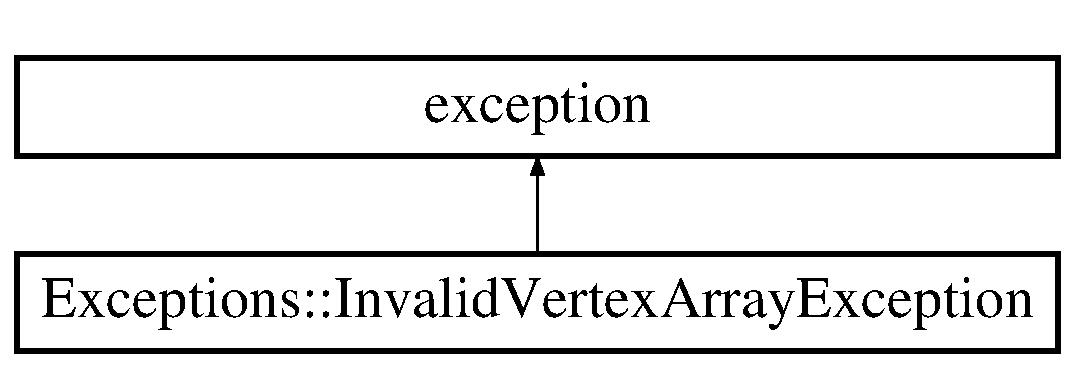
\includegraphics[height=2.000000cm]{class_exceptions_1_1_invalid_vertex_array_exception}
\end{center}
\end{figure}
\subsection*{Public Member Functions}
\begin{DoxyCompactItemize}
\item 
\hyperlink{class_exceptions_1_1_invalid_vertex_array_exception_a57cb1b8e280dc527308131a3409db516}{Invalid\+Vertex\+Array\+Exception} (const unsigned int \hyperlink{class_exceptions_1_1_invalid_vertex_array_exception_a600d7d65a0f48fe31c3de57a71766f1b}{vertex\+\_\+array\+\_\+binding})
\item 
virtual const char $\ast$ \hyperlink{class_exceptions_1_1_invalid_vertex_array_exception_a44652236482a680409b0db535c26bfa7}{what} () const   throw ()
\end{DoxyCompactItemize}
\subsection*{Private Attributes}
\begin{DoxyCompactItemize}
\item 
unsigned int \hyperlink{class_exceptions_1_1_invalid_vertex_array_exception_a600d7d65a0f48fe31c3de57a71766f1b}{vertex\+\_\+array\+\_\+binding}
\end{DoxyCompactItemize}


\subsection{Constructor \& Destructor Documentation}
\hypertarget{class_exceptions_1_1_invalid_vertex_array_exception_a57cb1b8e280dc527308131a3409db516}{}\index{Exceptions\+::\+Invalid\+Vertex\+Array\+Exception@{Exceptions\+::\+Invalid\+Vertex\+Array\+Exception}!Invalid\+Vertex\+Array\+Exception@{Invalid\+Vertex\+Array\+Exception}}
\index{Invalid\+Vertex\+Array\+Exception@{Invalid\+Vertex\+Array\+Exception}!Exceptions\+::\+Invalid\+Vertex\+Array\+Exception@{Exceptions\+::\+Invalid\+Vertex\+Array\+Exception}}
\subsubsection[{Invalid\+Vertex\+Array\+Exception}]{\setlength{\rightskip}{0pt plus 5cm}Exceptions\+::\+Invalid\+Vertex\+Array\+Exception\+::\+Invalid\+Vertex\+Array\+Exception (
\begin{DoxyParamCaption}
\item[{const unsigned int}]{vertex\+\_\+array\+\_\+binding}
\end{DoxyParamCaption}
)\hspace{0.3cm}{\ttfamily [inline]}}\label{class_exceptions_1_1_invalid_vertex_array_exception_a57cb1b8e280dc527308131a3409db516}


\subsection{Member Function Documentation}
\hypertarget{class_exceptions_1_1_invalid_vertex_array_exception_a44652236482a680409b0db535c26bfa7}{}\index{Exceptions\+::\+Invalid\+Vertex\+Array\+Exception@{Exceptions\+::\+Invalid\+Vertex\+Array\+Exception}!what@{what}}
\index{what@{what}!Exceptions\+::\+Invalid\+Vertex\+Array\+Exception@{Exceptions\+::\+Invalid\+Vertex\+Array\+Exception}}
\subsubsection[{what}]{\setlength{\rightskip}{0pt plus 5cm}virtual const char$\ast$ Exceptions\+::\+Invalid\+Vertex\+Array\+Exception\+::what (
\begin{DoxyParamCaption}
{}
\end{DoxyParamCaption}
) const throw  ) \hspace{0.3cm}{\ttfamily [inline]}, {\ttfamily [virtual]}}\label{class_exceptions_1_1_invalid_vertex_array_exception_a44652236482a680409b0db535c26bfa7}


\subsection{Member Data Documentation}
\hypertarget{class_exceptions_1_1_invalid_vertex_array_exception_a600d7d65a0f48fe31c3de57a71766f1b}{}\index{Exceptions\+::\+Invalid\+Vertex\+Array\+Exception@{Exceptions\+::\+Invalid\+Vertex\+Array\+Exception}!vertex\+\_\+array\+\_\+binding@{vertex\+\_\+array\+\_\+binding}}
\index{vertex\+\_\+array\+\_\+binding@{vertex\+\_\+array\+\_\+binding}!Exceptions\+::\+Invalid\+Vertex\+Array\+Exception@{Exceptions\+::\+Invalid\+Vertex\+Array\+Exception}}
\subsubsection[{vertex\+\_\+array\+\_\+binding}]{\setlength{\rightskip}{0pt plus 5cm}unsigned int Exceptions\+::\+Invalid\+Vertex\+Array\+Exception\+::vertex\+\_\+array\+\_\+binding\hspace{0.3cm}{\ttfamily [private]}}\label{class_exceptions_1_1_invalid_vertex_array_exception_a600d7d65a0f48fe31c3de57a71766f1b}


The documentation for this class was generated from the following file\+:\begin{DoxyCompactItemize}
\item 
src/exceptions/\hyperlink{invalid__vertex__array__exception_8h}{invalid\+\_\+vertex\+\_\+array\+\_\+exception.\+h}\end{DoxyCompactItemize}

\hypertarget{class_exceptions_1_1_invalid_vertex_shader_exception}{}\section{Exceptions\+:\+:Invalid\+Vertex\+Shader\+Exception Class Reference}
\label{class_exceptions_1_1_invalid_vertex_shader_exception}\index{Exceptions\+::\+Invalid\+Vertex\+Shader\+Exception@{Exceptions\+::\+Invalid\+Vertex\+Shader\+Exception}}


{\ttfamily \#include $<$invalid\+\_\+vertex\+\_\+shader\+\_\+exception.\+h$>$}

Inheritance diagram for Exceptions\+:\+:Invalid\+Vertex\+Shader\+Exception\+:\begin{figure}[H]
\begin{center}
\leavevmode
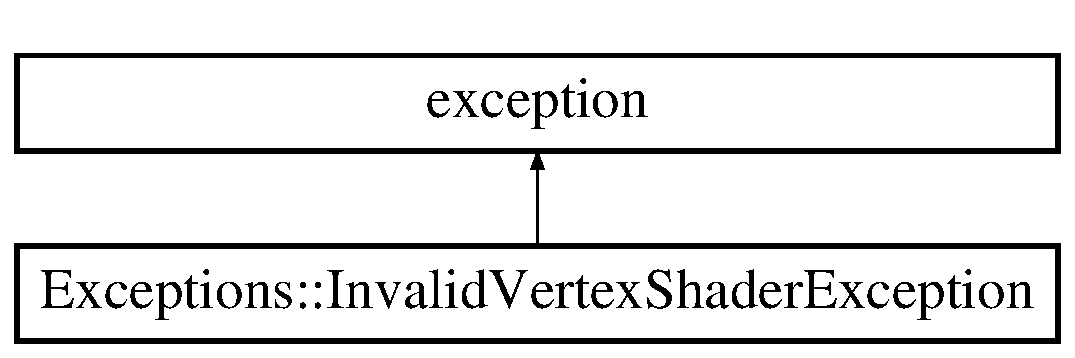
\includegraphics[height=2.000000cm]{class_exceptions_1_1_invalid_vertex_shader_exception}
\end{center}
\end{figure}
\subsection*{Public Member Functions}
\begin{DoxyCompactItemize}
\item 
\hyperlink{class_exceptions_1_1_invalid_vertex_shader_exception_a9ba81ea3e560d851ada643f0fdd8fefb}{Invalid\+Vertex\+Shader\+Exception} (const unsigned int \hyperlink{class_exceptions_1_1_invalid_vertex_shader_exception_a4bf93e6765dc1611a442cedc749ecb43}{vertex\+\_\+shader\+\_\+binding})
\item 
virtual const char $\ast$ \hyperlink{class_exceptions_1_1_invalid_vertex_shader_exception_a63b07be0e1e29b3f8f4c8f8cfb7eb735}{what} () const   throw ()
\end{DoxyCompactItemize}
\subsection*{Private Attributes}
\begin{DoxyCompactItemize}
\item 
unsigned int \hyperlink{class_exceptions_1_1_invalid_vertex_shader_exception_a4bf93e6765dc1611a442cedc749ecb43}{vertex\+\_\+shader\+\_\+binding}
\end{DoxyCompactItemize}


\subsection{Constructor \& Destructor Documentation}
\hypertarget{class_exceptions_1_1_invalid_vertex_shader_exception_a9ba81ea3e560d851ada643f0fdd8fefb}{}\index{Exceptions\+::\+Invalid\+Vertex\+Shader\+Exception@{Exceptions\+::\+Invalid\+Vertex\+Shader\+Exception}!Invalid\+Vertex\+Shader\+Exception@{Invalid\+Vertex\+Shader\+Exception}}
\index{Invalid\+Vertex\+Shader\+Exception@{Invalid\+Vertex\+Shader\+Exception}!Exceptions\+::\+Invalid\+Vertex\+Shader\+Exception@{Exceptions\+::\+Invalid\+Vertex\+Shader\+Exception}}
\subsubsection[{Invalid\+Vertex\+Shader\+Exception}]{\setlength{\rightskip}{0pt plus 5cm}Exceptions\+::\+Invalid\+Vertex\+Shader\+Exception\+::\+Invalid\+Vertex\+Shader\+Exception (
\begin{DoxyParamCaption}
\item[{const unsigned int}]{vertex\+\_\+shader\+\_\+binding}
\end{DoxyParamCaption}
)\hspace{0.3cm}{\ttfamily [inline]}}\label{class_exceptions_1_1_invalid_vertex_shader_exception_a9ba81ea3e560d851ada643f0fdd8fefb}


\subsection{Member Function Documentation}
\hypertarget{class_exceptions_1_1_invalid_vertex_shader_exception_a63b07be0e1e29b3f8f4c8f8cfb7eb735}{}\index{Exceptions\+::\+Invalid\+Vertex\+Shader\+Exception@{Exceptions\+::\+Invalid\+Vertex\+Shader\+Exception}!what@{what}}
\index{what@{what}!Exceptions\+::\+Invalid\+Vertex\+Shader\+Exception@{Exceptions\+::\+Invalid\+Vertex\+Shader\+Exception}}
\subsubsection[{what}]{\setlength{\rightskip}{0pt plus 5cm}virtual const char$\ast$ Exceptions\+::\+Invalid\+Vertex\+Shader\+Exception\+::what (
\begin{DoxyParamCaption}
{}
\end{DoxyParamCaption}
) const throw  ) \hspace{0.3cm}{\ttfamily [inline]}, {\ttfamily [virtual]}}\label{class_exceptions_1_1_invalid_vertex_shader_exception_a63b07be0e1e29b3f8f4c8f8cfb7eb735}


\subsection{Member Data Documentation}
\hypertarget{class_exceptions_1_1_invalid_vertex_shader_exception_a4bf93e6765dc1611a442cedc749ecb43}{}\index{Exceptions\+::\+Invalid\+Vertex\+Shader\+Exception@{Exceptions\+::\+Invalid\+Vertex\+Shader\+Exception}!vertex\+\_\+shader\+\_\+binding@{vertex\+\_\+shader\+\_\+binding}}
\index{vertex\+\_\+shader\+\_\+binding@{vertex\+\_\+shader\+\_\+binding}!Exceptions\+::\+Invalid\+Vertex\+Shader\+Exception@{Exceptions\+::\+Invalid\+Vertex\+Shader\+Exception}}
\subsubsection[{vertex\+\_\+shader\+\_\+binding}]{\setlength{\rightskip}{0pt plus 5cm}unsigned int Exceptions\+::\+Invalid\+Vertex\+Shader\+Exception\+::vertex\+\_\+shader\+\_\+binding\hspace{0.3cm}{\ttfamily [private]}}\label{class_exceptions_1_1_invalid_vertex_shader_exception_a4bf93e6765dc1611a442cedc749ecb43}


The documentation for this class was generated from the following file\+:\begin{DoxyCompactItemize}
\item 
src/exceptions/\hyperlink{invalid__vertex__shader__exception_8h}{invalid\+\_\+vertex\+\_\+shader\+\_\+exception.\+h}\end{DoxyCompactItemize}

\hypertarget{class_graphics_1_1_renderable}{}\section{Graphics\+:\+:Renderable Class Reference}
\label{class_graphics_1_1_renderable}\index{Graphics\+::\+Renderable@{Graphics\+::\+Renderable}}


{\ttfamily \#include $<$renderable.\+h$>$}

Inheritance diagram for Graphics\+:\+:Renderable\+:\begin{figure}[H]
\begin{center}
\leavevmode
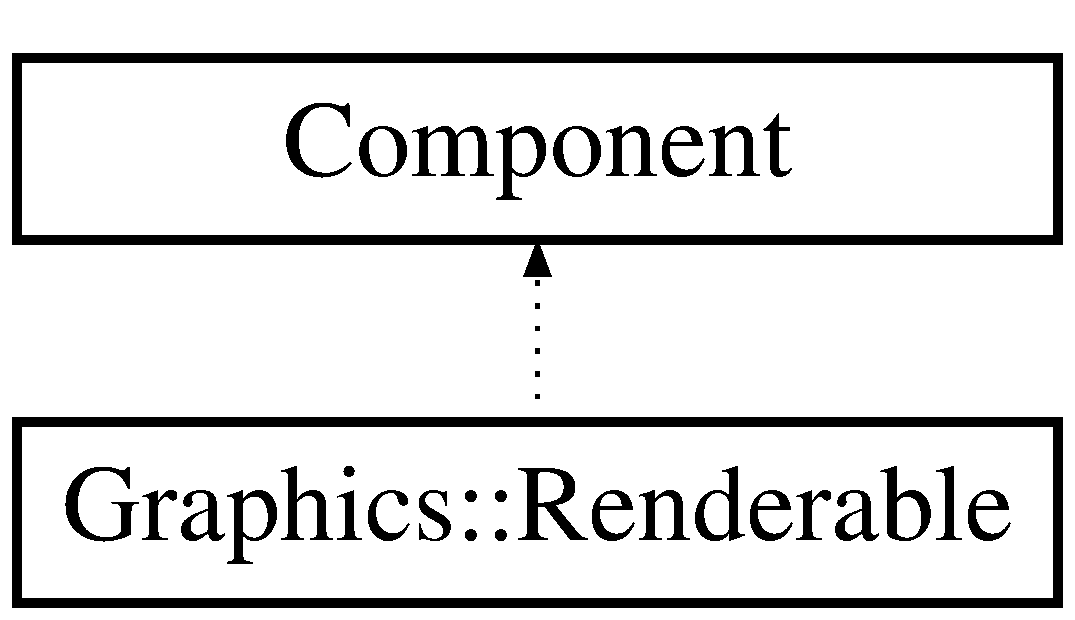
\includegraphics[height=4.000000cm]{class_graphics_1_1_renderable}
\end{center}
\end{figure}
\subsection*{Public Member Functions}
\begin{DoxyCompactItemize}
\item 
\hyperlink{class_graphics_1_1_renderable_a2c99d41631558194811f6f4c61a7f464}{Renderable} ()=delete
\item 
\hyperlink{class_graphics_1_1_renderable_a08ba323265fd34d219ed3495ee255c9b}{Renderable} (const unsigned int \hyperlink{class_graphics_1_1_renderable_aabfa91ebff7b10decd54119d663044ef}{vertex\+\_\+array\+\_\+object}, const \hyperlink{class_graphics_1_1_vertex_data}{Vertex\+Data} \&\hyperlink{class_graphics_1_1_renderable_a5077fe6a71021f0bd4ebc8d24cdf544b}{vertex\+\_\+data}, \hyperlink{class_graphics_1_1_base_attribute_trait}{Base\+Attribute\+Trait} $\ast$\hyperlink{class_graphics_1_1_renderable_a27f39fbb4866ccfc83f0662a59c03020}{trait}=new \hyperlink{class_graphics_1_1_renderable_attribute_trait}{Renderable\+Attribute\+Trait}())
\item 
\hyperlink{class_graphics_1_1_renderable_a7db48c39efa99650480cca6376bbf6c6}{Renderable} (const \hyperlink{class_graphics_1_1_renderable}{Renderable} \&)=delete
\item 
\hyperlink{class_graphics_1_1_renderable}{Renderable} \hyperlink{class_graphics_1_1_renderable_aa96e579c501d01462f5ee2ed5e949311}{operator=} (\hyperlink{class_graphics_1_1_renderable}{Renderable} \&)=delete
\item 
\hyperlink{class_graphics_1_1_renderable_a7edf9a0c89593ab500d5107e89f7bbae}{Renderable} (\hyperlink{class_graphics_1_1_renderable}{Renderable} \&\&renderable)
\item 
\hyperlink{class_graphics_1_1_renderable}{Renderable} \& \hyperlink{class_graphics_1_1_renderable_afac6ce4fffafffef11300fd13b763ef4}{operator=} (\hyperlink{class_graphics_1_1_renderable}{Renderable} \&\&renderable)
\item 
virtual \hyperlink{class_graphics_1_1_renderable_a63470b6e63ed9f87690569833fb48617}{$\sim$\+Renderable} ()
\item 
void \hyperlink{class_graphics_1_1_renderable_aab2e51991d63780654d7cc8a7083faca}{set\+Active} () noexcept
\item 
void \hyperlink{class_graphics_1_1_renderable_a9b6b9bf46beb9e4df9a0ba1dae55b87e}{set\+Inactive} () noexcept
\item 
const bool \hyperlink{class_graphics_1_1_renderable_a3ee6ae0274eaed19b731a97c5b44d2d6}{is\+Active} () const noexcept
\item 
void \hyperlink{class_graphics_1_1_renderable_a481dfc871e6129e8ee55482207ddc7fa}{set\+Shader} (std\+::shared\+\_\+ptr$<$ \hyperlink{class_graphics_1_1_shader}{Shader} $>$ shader\+\_\+object) noexcept
\item 
const std\+::shared\+\_\+ptr$<$ \hyperlink{class_graphics_1_1_shader}{Shader} $>$ \hyperlink{class_graphics_1_1_renderable_a542b918d1c6375ffdd06881d3fc31edd}{get\+Shader} () const noexcept
\item 
void \hyperlink{class_graphics_1_1_renderable_a8014f2c976291a09d452330448ca72d6}{add\+Texture} (std\+::shared\+\_\+ptr$<$ \hyperlink{class_graphics_1_1_base_texture}{Base\+Texture} $>$ texture\+\_\+object) noexcept
\item 
const std\+::vector$<$ std\+::shared\+\_\+ptr$<$ \hyperlink{class_graphics_1_1_base_texture}{Base\+Texture} $>$ $>$ \hyperlink{class_graphics_1_1_renderable_ac1634b94ac82b2b470010a3221c15643}{get\+Textures} () const noexcept
\item 
const std\+::shared\+\_\+ptr$<$ \hyperlink{class_graphics_1_1_base_texture}{Base\+Texture} $>$ \hyperlink{class_graphics_1_1_renderable_a9d134bc92527be7b68c65c8e5d70d8c0}{get\+Texture\+By\+Uniform} (const std\+::string \&uniform\+\_\+name)
\item 
void \hyperlink{class_graphics_1_1_renderable_a0166ebd26cac50f87ec7a33c5db9a3c5}{set\+Light\+Reactive} (const bool reactive) noexcept
\item 
const bool \hyperlink{class_graphics_1_1_renderable_a066fd1f919bdc7f2e562419f3e512dcd}{is\+Light\+Reactive} () const noexcept
\item 
void \hyperlink{class_graphics_1_1_renderable_ae50c65b85cb389df96b8e913b6dfe580}{set\+Ambient\+Light} (const glm\+::vec3 color) noexcept
\item 
const glm\+::vec3 \hyperlink{class_graphics_1_1_renderable_a9c000568c9df44433eceb76c5f1e39c0}{get\+Ambient\+Light} () const noexcept
\item 
void \hyperlink{class_graphics_1_1_renderable_acd1b9f38205aa1a637c46fe7faeed60c}{set\+Ambient\+Intensity} (const float intensity) noexcept
\item 
const float \hyperlink{class_graphics_1_1_renderable_a678da7336bb38a8cab7edf423f6dfed5}{get\+Ambient\+Intensity} () const noexcept
\item 
void \hyperlink{class_graphics_1_1_renderable_aa33e801d00279049d15e1a133f76eaf4}{add\+Influencing\+Light} (std\+::shared\+\_\+ptr$<$ \hyperlink{class_graphics_1_1_light}{Light} $>$ light) noexcept
\item 
void \hyperlink{class_graphics_1_1_renderable_a448be1ad2063cb3ff8b901a94ae0b566}{clear\+Influencing\+Lights} ()
\item 
const unsigned int \hyperlink{class_graphics_1_1_renderable_afde066c6e5ab15ce9b055f9f8f4593ff}{get\+Vertex\+Array\+Binding} () const noexcept
\item 
const \hyperlink{class_graphics_1_1_vertex_data}{Vertex\+Data} \hyperlink{class_graphics_1_1_renderable_a1d304b7063ae0acdef62b8041258a10b}{get\+Vertex\+Data} () const noexcept
\item 
virtual void \hyperlink{class_graphics_1_1_renderable_a6e20996de55215db7ffae2792aaaa88e}{on\+Destroy} () override
\item 
virtual void \hyperlink{class_graphics_1_1_renderable_a7433551970cd25e0241a4a5bb756ba50}{on\+Start} () override
\item 
virtual const bool \hyperlink{class_graphics_1_1_renderable_a7d0e820c55cb7f5c552aa0c1e846db76}{on\+Update} (const double delta) override
\begin{DoxyCompactList}\small\item\em \mbox{[}brief description\mbox{]} \end{DoxyCompactList}\item 
virtual const bool \hyperlink{class_graphics_1_1_renderable_afafd0e6147c73090234670934bbb8cbb}{on\+Render} ()
\end{DoxyCompactItemize}
\subsection*{Private Attributes}
\begin{DoxyCompactItemize}
\item 
bool \hyperlink{class_graphics_1_1_renderable_a5ee90a804fea73ddfaeed77086ecead4}{active}
\item 
unsigned int \hyperlink{class_graphics_1_1_renderable_aabfa91ebff7b10decd54119d663044ef}{vertex\+\_\+array\+\_\+object}
\item 
std\+::shared\+\_\+ptr$<$ \hyperlink{class_graphics_1_1_shader}{Shader} $>$ \hyperlink{class_graphics_1_1_renderable_a6c951dfc9a00d3f3f79550112d0f40e3}{shader}
\item 
std\+::vector$<$ std\+::shared\+\_\+ptr$<$ \hyperlink{class_graphics_1_1_base_texture}{Base\+Texture} $>$ $>$ \hyperlink{class_graphics_1_1_renderable_ac3a09a4fbb226022792d8abf07ff549a}{textures}
\item 
\hyperlink{class_graphics_1_1_vertex_data}{Vertex\+Data} \hyperlink{class_graphics_1_1_renderable_a5077fe6a71021f0bd4ebc8d24cdf544b}{vertex\+\_\+data}
\item 
std\+::unique\+\_\+ptr$<$ \hyperlink{class_graphics_1_1_base_attribute_trait}{Base\+Attribute\+Trait} $>$ \hyperlink{class_graphics_1_1_renderable_a27f39fbb4866ccfc83f0662a59c03020}{trait}
\item 
bool \hyperlink{class_graphics_1_1_renderable_a4a0fd8d55a1881c2b41e854ddb78366a}{light\+\_\+reactive}
\item 
std\+::list$<$ std\+::shared\+\_\+ptr$<$ \hyperlink{class_graphics_1_1_light}{Light} $>$ $>$ \hyperlink{class_graphics_1_1_renderable_a45bf29c03f8d47d870c6a1ce44126007}{influencing\+\_\+lights}
\item 
glm\+::vec3 \hyperlink{class_graphics_1_1_renderable_aecd9a143f7abb6c6b4969c147ee245c3}{ambient\+\_\+light}
\item 
float \hyperlink{class_graphics_1_1_renderable_a52fb337984cab44bb827037c9c13956e}{ambient\+\_\+intensity}
\end{DoxyCompactItemize}
\subsection*{Additional Inherited Members}


\subsection{Constructor \& Destructor Documentation}
\hypertarget{class_graphics_1_1_renderable_a2c99d41631558194811f6f4c61a7f464}{}\index{Graphics\+::\+Renderable@{Graphics\+::\+Renderable}!Renderable@{Renderable}}
\index{Renderable@{Renderable}!Graphics\+::\+Renderable@{Graphics\+::\+Renderable}}
\subsubsection[{Renderable}]{\setlength{\rightskip}{0pt plus 5cm}Graphics\+::\+Renderable\+::\+Renderable (
\begin{DoxyParamCaption}
{}
\end{DoxyParamCaption}
)\hspace{0.3cm}{\ttfamily [delete]}}\label{class_graphics_1_1_renderable_a2c99d41631558194811f6f4c61a7f464}
\hypertarget{class_graphics_1_1_renderable_a08ba323265fd34d219ed3495ee255c9b}{}\index{Graphics\+::\+Renderable@{Graphics\+::\+Renderable}!Renderable@{Renderable}}
\index{Renderable@{Renderable}!Graphics\+::\+Renderable@{Graphics\+::\+Renderable}}
\subsubsection[{Renderable}]{\setlength{\rightskip}{0pt plus 5cm}Graphics\+::\+Renderable\+::\+Renderable (
\begin{DoxyParamCaption}
\item[{const unsigned int}]{vertex\+\_\+array\+\_\+object, }
\item[{const {\bf Vertex\+Data} \&}]{vertex\+\_\+data, }
\item[{{\bf Base\+Attribute\+Trait} $\ast$}]{trait = {\ttfamily new~{\bf Renderable\+Attribute\+Trait}()}}
\end{DoxyParamCaption}
)}\label{class_graphics_1_1_renderable_a08ba323265fd34d219ed3495ee255c9b}
\hypertarget{class_graphics_1_1_renderable_a7db48c39efa99650480cca6376bbf6c6}{}\index{Graphics\+::\+Renderable@{Graphics\+::\+Renderable}!Renderable@{Renderable}}
\index{Renderable@{Renderable}!Graphics\+::\+Renderable@{Graphics\+::\+Renderable}}
\subsubsection[{Renderable}]{\setlength{\rightskip}{0pt plus 5cm}Graphics\+::\+Renderable\+::\+Renderable (
\begin{DoxyParamCaption}
\item[{const {\bf Renderable} \&}]{}
\end{DoxyParamCaption}
)\hspace{0.3cm}{\ttfamily [delete]}}\label{class_graphics_1_1_renderable_a7db48c39efa99650480cca6376bbf6c6}
\hypertarget{class_graphics_1_1_renderable_a7edf9a0c89593ab500d5107e89f7bbae}{}\index{Graphics\+::\+Renderable@{Graphics\+::\+Renderable}!Renderable@{Renderable}}
\index{Renderable@{Renderable}!Graphics\+::\+Renderable@{Graphics\+::\+Renderable}}
\subsubsection[{Renderable}]{\setlength{\rightskip}{0pt plus 5cm}Graphics\+::\+Renderable\+::\+Renderable (
\begin{DoxyParamCaption}
\item[{{\bf Renderable} \&\&}]{renderable}
\end{DoxyParamCaption}
)}\label{class_graphics_1_1_renderable_a7edf9a0c89593ab500d5107e89f7bbae}
\hypertarget{class_graphics_1_1_renderable_a63470b6e63ed9f87690569833fb48617}{}\index{Graphics\+::\+Renderable@{Graphics\+::\+Renderable}!````~Renderable@{$\sim$\+Renderable}}
\index{````~Renderable@{$\sim$\+Renderable}!Graphics\+::\+Renderable@{Graphics\+::\+Renderable}}
\subsubsection[{$\sim$\+Renderable}]{\setlength{\rightskip}{0pt plus 5cm}Graphics\+::\+Renderable\+::$\sim$\+Renderable (
\begin{DoxyParamCaption}
{}
\end{DoxyParamCaption}
)\hspace{0.3cm}{\ttfamily [virtual]}}\label{class_graphics_1_1_renderable_a63470b6e63ed9f87690569833fb48617}


\subsection{Member Function Documentation}
\hypertarget{class_graphics_1_1_renderable_aa33e801d00279049d15e1a133f76eaf4}{}\index{Graphics\+::\+Renderable@{Graphics\+::\+Renderable}!add\+Influencing\+Light@{add\+Influencing\+Light}}
\index{add\+Influencing\+Light@{add\+Influencing\+Light}!Graphics\+::\+Renderable@{Graphics\+::\+Renderable}}
\subsubsection[{add\+Influencing\+Light}]{\setlength{\rightskip}{0pt plus 5cm}void Graphics\+::\+Renderable\+::add\+Influencing\+Light (
\begin{DoxyParamCaption}
\item[{std\+::shared\+\_\+ptr$<$ {\bf Light} $>$}]{light}
\end{DoxyParamCaption}
)\hspace{0.3cm}{\ttfamily [noexcept]}}\label{class_graphics_1_1_renderable_aa33e801d00279049d15e1a133f76eaf4}
\hypertarget{class_graphics_1_1_renderable_a8014f2c976291a09d452330448ca72d6}{}\index{Graphics\+::\+Renderable@{Graphics\+::\+Renderable}!add\+Texture@{add\+Texture}}
\index{add\+Texture@{add\+Texture}!Graphics\+::\+Renderable@{Graphics\+::\+Renderable}}
\subsubsection[{add\+Texture}]{\setlength{\rightskip}{0pt plus 5cm}void Graphics\+::\+Renderable\+::add\+Texture (
\begin{DoxyParamCaption}
\item[{std\+::shared\+\_\+ptr$<$ {\bf Base\+Texture} $>$}]{texture\+\_\+object}
\end{DoxyParamCaption}
)\hspace{0.3cm}{\ttfamily [noexcept]}}\label{class_graphics_1_1_renderable_a8014f2c976291a09d452330448ca72d6}
\hypertarget{class_graphics_1_1_renderable_a448be1ad2063cb3ff8b901a94ae0b566}{}\index{Graphics\+::\+Renderable@{Graphics\+::\+Renderable}!clear\+Influencing\+Lights@{clear\+Influencing\+Lights}}
\index{clear\+Influencing\+Lights@{clear\+Influencing\+Lights}!Graphics\+::\+Renderable@{Graphics\+::\+Renderable}}
\subsubsection[{clear\+Influencing\+Lights}]{\setlength{\rightskip}{0pt plus 5cm}void Graphics\+::\+Renderable\+::clear\+Influencing\+Lights (
\begin{DoxyParamCaption}
{}
\end{DoxyParamCaption}
)}\label{class_graphics_1_1_renderable_a448be1ad2063cb3ff8b901a94ae0b566}
\hypertarget{class_graphics_1_1_renderable_a678da7336bb38a8cab7edf423f6dfed5}{}\index{Graphics\+::\+Renderable@{Graphics\+::\+Renderable}!get\+Ambient\+Intensity@{get\+Ambient\+Intensity}}
\index{get\+Ambient\+Intensity@{get\+Ambient\+Intensity}!Graphics\+::\+Renderable@{Graphics\+::\+Renderable}}
\subsubsection[{get\+Ambient\+Intensity}]{\setlength{\rightskip}{0pt plus 5cm}const float Graphics\+::\+Renderable\+::get\+Ambient\+Intensity (
\begin{DoxyParamCaption}
{}
\end{DoxyParamCaption}
) const\hspace{0.3cm}{\ttfamily [noexcept]}}\label{class_graphics_1_1_renderable_a678da7336bb38a8cab7edf423f6dfed5}
\hypertarget{class_graphics_1_1_renderable_a9c000568c9df44433eceb76c5f1e39c0}{}\index{Graphics\+::\+Renderable@{Graphics\+::\+Renderable}!get\+Ambient\+Light@{get\+Ambient\+Light}}
\index{get\+Ambient\+Light@{get\+Ambient\+Light}!Graphics\+::\+Renderable@{Graphics\+::\+Renderable}}
\subsubsection[{get\+Ambient\+Light}]{\setlength{\rightskip}{0pt plus 5cm}const glm\+::vec3 Graphics\+::\+Renderable\+::get\+Ambient\+Light (
\begin{DoxyParamCaption}
{}
\end{DoxyParamCaption}
) const\hspace{0.3cm}{\ttfamily [noexcept]}}\label{class_graphics_1_1_renderable_a9c000568c9df44433eceb76c5f1e39c0}
\hypertarget{class_graphics_1_1_renderable_a542b918d1c6375ffdd06881d3fc31edd}{}\index{Graphics\+::\+Renderable@{Graphics\+::\+Renderable}!get\+Shader@{get\+Shader}}
\index{get\+Shader@{get\+Shader}!Graphics\+::\+Renderable@{Graphics\+::\+Renderable}}
\subsubsection[{get\+Shader}]{\setlength{\rightskip}{0pt plus 5cm}const std\+::shared\+\_\+ptr$<$ {\bf Shader} $>$ Graphics\+::\+Renderable\+::get\+Shader (
\begin{DoxyParamCaption}
{}
\end{DoxyParamCaption}
) const\hspace{0.3cm}{\ttfamily [noexcept]}}\label{class_graphics_1_1_renderable_a542b918d1c6375ffdd06881d3fc31edd}
\hypertarget{class_graphics_1_1_renderable_a9d134bc92527be7b68c65c8e5d70d8c0}{}\index{Graphics\+::\+Renderable@{Graphics\+::\+Renderable}!get\+Texture\+By\+Uniform@{get\+Texture\+By\+Uniform}}
\index{get\+Texture\+By\+Uniform@{get\+Texture\+By\+Uniform}!Graphics\+::\+Renderable@{Graphics\+::\+Renderable}}
\subsubsection[{get\+Texture\+By\+Uniform}]{\setlength{\rightskip}{0pt plus 5cm}const std\+::shared\+\_\+ptr$<$ {\bf Base\+Texture} $>$ Graphics\+::\+Renderable\+::get\+Texture\+By\+Uniform (
\begin{DoxyParamCaption}
\item[{const std\+::string \&}]{uniform\+\_\+name}
\end{DoxyParamCaption}
)}\label{class_graphics_1_1_renderable_a9d134bc92527be7b68c65c8e5d70d8c0}
\hypertarget{class_graphics_1_1_renderable_ac1634b94ac82b2b470010a3221c15643}{}\index{Graphics\+::\+Renderable@{Graphics\+::\+Renderable}!get\+Textures@{get\+Textures}}
\index{get\+Textures@{get\+Textures}!Graphics\+::\+Renderable@{Graphics\+::\+Renderable}}
\subsubsection[{get\+Textures}]{\setlength{\rightskip}{0pt plus 5cm}const std\+::vector$<$ std\+::shared\+\_\+ptr$<$ {\bf Base\+Texture} $>$ $>$ Graphics\+::\+Renderable\+::get\+Textures (
\begin{DoxyParamCaption}
{}
\end{DoxyParamCaption}
) const\hspace{0.3cm}{\ttfamily [noexcept]}}\label{class_graphics_1_1_renderable_ac1634b94ac82b2b470010a3221c15643}
\hypertarget{class_graphics_1_1_renderable_afde066c6e5ab15ce9b055f9f8f4593ff}{}\index{Graphics\+::\+Renderable@{Graphics\+::\+Renderable}!get\+Vertex\+Array\+Binding@{get\+Vertex\+Array\+Binding}}
\index{get\+Vertex\+Array\+Binding@{get\+Vertex\+Array\+Binding}!Graphics\+::\+Renderable@{Graphics\+::\+Renderable}}
\subsubsection[{get\+Vertex\+Array\+Binding}]{\setlength{\rightskip}{0pt plus 5cm}const unsigned int Graphics\+::\+Renderable\+::get\+Vertex\+Array\+Binding (
\begin{DoxyParamCaption}
{}
\end{DoxyParamCaption}
) const\hspace{0.3cm}{\ttfamily [noexcept]}}\label{class_graphics_1_1_renderable_afde066c6e5ab15ce9b055f9f8f4593ff}
\hypertarget{class_graphics_1_1_renderable_a1d304b7063ae0acdef62b8041258a10b}{}\index{Graphics\+::\+Renderable@{Graphics\+::\+Renderable}!get\+Vertex\+Data@{get\+Vertex\+Data}}
\index{get\+Vertex\+Data@{get\+Vertex\+Data}!Graphics\+::\+Renderable@{Graphics\+::\+Renderable}}
\subsubsection[{get\+Vertex\+Data}]{\setlength{\rightskip}{0pt plus 5cm}const {\bf Vertex\+Data} Graphics\+::\+Renderable\+::get\+Vertex\+Data (
\begin{DoxyParamCaption}
{}
\end{DoxyParamCaption}
) const\hspace{0.3cm}{\ttfamily [noexcept]}}\label{class_graphics_1_1_renderable_a1d304b7063ae0acdef62b8041258a10b}
\hypertarget{class_graphics_1_1_renderable_a3ee6ae0274eaed19b731a97c5b44d2d6}{}\index{Graphics\+::\+Renderable@{Graphics\+::\+Renderable}!is\+Active@{is\+Active}}
\index{is\+Active@{is\+Active}!Graphics\+::\+Renderable@{Graphics\+::\+Renderable}}
\subsubsection[{is\+Active}]{\setlength{\rightskip}{0pt plus 5cm}const bool Graphics\+::\+Renderable\+::is\+Active (
\begin{DoxyParamCaption}
{}
\end{DoxyParamCaption}
) const\hspace{0.3cm}{\ttfamily [noexcept]}}\label{class_graphics_1_1_renderable_a3ee6ae0274eaed19b731a97c5b44d2d6}
\hypertarget{class_graphics_1_1_renderable_a066fd1f919bdc7f2e562419f3e512dcd}{}\index{Graphics\+::\+Renderable@{Graphics\+::\+Renderable}!is\+Light\+Reactive@{is\+Light\+Reactive}}
\index{is\+Light\+Reactive@{is\+Light\+Reactive}!Graphics\+::\+Renderable@{Graphics\+::\+Renderable}}
\subsubsection[{is\+Light\+Reactive}]{\setlength{\rightskip}{0pt plus 5cm}const bool Graphics\+::\+Renderable\+::is\+Light\+Reactive (
\begin{DoxyParamCaption}
{}
\end{DoxyParamCaption}
) const\hspace{0.3cm}{\ttfamily [noexcept]}}\label{class_graphics_1_1_renderable_a066fd1f919bdc7f2e562419f3e512dcd}
\hypertarget{class_graphics_1_1_renderable_a6e20996de55215db7ffae2792aaaa88e}{}\index{Graphics\+::\+Renderable@{Graphics\+::\+Renderable}!on\+Destroy@{on\+Destroy}}
\index{on\+Destroy@{on\+Destroy}!Graphics\+::\+Renderable@{Graphics\+::\+Renderable}}
\subsubsection[{on\+Destroy}]{\setlength{\rightskip}{0pt plus 5cm}void Graphics\+::\+Renderable\+::on\+Destroy (
\begin{DoxyParamCaption}
{}
\end{DoxyParamCaption}
)\hspace{0.3cm}{\ttfamily [override]}, {\ttfamily [virtual]}}\label{class_graphics_1_1_renderable_a6e20996de55215db7ffae2792aaaa88e}


Implements \hyperlink{class_component_a2b198f27162a6caf63917e304295f892}{Component}.



Reimplemented in \hyperlink{class_graphics_1_1_animated_tile_a9781b9b256a666a123fd2c050adb5118}{Graphics\+::\+Animated\+Tile}, and \hyperlink{class_graphics_1_1_tile_a28f5bdfa2fc61b292dda7ec15316b981}{Graphics\+::\+Tile}.

\hypertarget{class_graphics_1_1_renderable_afafd0e6147c73090234670934bbb8cbb}{}\index{Graphics\+::\+Renderable@{Graphics\+::\+Renderable}!on\+Render@{on\+Render}}
\index{on\+Render@{on\+Render}!Graphics\+::\+Renderable@{Graphics\+::\+Renderable}}
\subsubsection[{on\+Render}]{\setlength{\rightskip}{0pt plus 5cm}const bool Graphics\+::\+Renderable\+::on\+Render (
\begin{DoxyParamCaption}
{}
\end{DoxyParamCaption}
)\hspace{0.3cm}{\ttfamily [virtual]}}\label{class_graphics_1_1_renderable_afafd0e6147c73090234670934bbb8cbb}


Reimplemented in \hyperlink{class_graphics_1_1_animated_tile_a0b414dfdb18e4647652f8bb9334f9eee}{Graphics\+::\+Animated\+Tile}.

\hypertarget{class_graphics_1_1_renderable_a7433551970cd25e0241a4a5bb756ba50}{}\index{Graphics\+::\+Renderable@{Graphics\+::\+Renderable}!on\+Start@{on\+Start}}
\index{on\+Start@{on\+Start}!Graphics\+::\+Renderable@{Graphics\+::\+Renderable}}
\subsubsection[{on\+Start}]{\setlength{\rightskip}{0pt plus 5cm}void Graphics\+::\+Renderable\+::on\+Start (
\begin{DoxyParamCaption}
{}
\end{DoxyParamCaption}
)\hspace{0.3cm}{\ttfamily [override]}, {\ttfamily [virtual]}}\label{class_graphics_1_1_renderable_a7433551970cd25e0241a4a5bb756ba50}


Implements \hyperlink{class_component_a4a528a8790dbc141ffd0aba638b6dcc4}{Component}.



Reimplemented in \hyperlink{class_graphics_1_1_animated_tile_ad82e39321244cc2e06ee3df527473aba}{Graphics\+::\+Animated\+Tile}.

\hypertarget{class_graphics_1_1_renderable_a7d0e820c55cb7f5c552aa0c1e846db76}{}\index{Graphics\+::\+Renderable@{Graphics\+::\+Renderable}!on\+Update@{on\+Update}}
\index{on\+Update@{on\+Update}!Graphics\+::\+Renderable@{Graphics\+::\+Renderable}}
\subsubsection[{on\+Update}]{\setlength{\rightskip}{0pt plus 5cm}const bool Graphics\+::\+Renderable\+::on\+Update (
\begin{DoxyParamCaption}
\item[{const double}]{delta}
\end{DoxyParamCaption}
)\hspace{0.3cm}{\ttfamily [override]}, {\ttfamily [virtual]}}\label{class_graphics_1_1_renderable_a7d0e820c55cb7f5c552aa0c1e846db76}


\mbox{[}brief description\mbox{]} 

\mbox{[}long description\mbox{]} \begin{DoxyReturn}{Returns}
true if anything was updated, false if nothing was updated 
\end{DoxyReturn}


Implements \hyperlink{class_component_a8be284fccf4e97cee6705bd2d8f3705e}{Component}.



Reimplemented in \hyperlink{class_graphics_1_1_animated_tile_a2c6f7cd3866cad84b73ea5da8b92b76e}{Graphics\+::\+Animated\+Tile}, and \hyperlink{class_graphics_1_1_tile_a0311b1d9548f6badc9e81820b110cbb4}{Graphics\+::\+Tile}.

\hypertarget{class_graphics_1_1_renderable_aa96e579c501d01462f5ee2ed5e949311}{}\index{Graphics\+::\+Renderable@{Graphics\+::\+Renderable}!operator=@{operator=}}
\index{operator=@{operator=}!Graphics\+::\+Renderable@{Graphics\+::\+Renderable}}
\subsubsection[{operator=}]{\setlength{\rightskip}{0pt plus 5cm}{\bf Renderable} Graphics\+::\+Renderable\+::operator= (
\begin{DoxyParamCaption}
\item[{{\bf Renderable} \&}]{}
\end{DoxyParamCaption}
)\hspace{0.3cm}{\ttfamily [delete]}}\label{class_graphics_1_1_renderable_aa96e579c501d01462f5ee2ed5e949311}
\hypertarget{class_graphics_1_1_renderable_afac6ce4fffafffef11300fd13b763ef4}{}\index{Graphics\+::\+Renderable@{Graphics\+::\+Renderable}!operator=@{operator=}}
\index{operator=@{operator=}!Graphics\+::\+Renderable@{Graphics\+::\+Renderable}}
\subsubsection[{operator=}]{\setlength{\rightskip}{0pt plus 5cm}{\bf Renderable} \& Graphics\+::\+Renderable\+::operator= (
\begin{DoxyParamCaption}
\item[{{\bf Renderable} \&\&}]{renderable}
\end{DoxyParamCaption}
)}\label{class_graphics_1_1_renderable_afac6ce4fffafffef11300fd13b763ef4}
\hypertarget{class_graphics_1_1_renderable_aab2e51991d63780654d7cc8a7083faca}{}\index{Graphics\+::\+Renderable@{Graphics\+::\+Renderable}!set\+Active@{set\+Active}}
\index{set\+Active@{set\+Active}!Graphics\+::\+Renderable@{Graphics\+::\+Renderable}}
\subsubsection[{set\+Active}]{\setlength{\rightskip}{0pt plus 5cm}void Graphics\+::\+Renderable\+::set\+Active (
\begin{DoxyParamCaption}
{}
\end{DoxyParamCaption}
)\hspace{0.3cm}{\ttfamily [noexcept]}}\label{class_graphics_1_1_renderable_aab2e51991d63780654d7cc8a7083faca}
\hypertarget{class_graphics_1_1_renderable_acd1b9f38205aa1a637c46fe7faeed60c}{}\index{Graphics\+::\+Renderable@{Graphics\+::\+Renderable}!set\+Ambient\+Intensity@{set\+Ambient\+Intensity}}
\index{set\+Ambient\+Intensity@{set\+Ambient\+Intensity}!Graphics\+::\+Renderable@{Graphics\+::\+Renderable}}
\subsubsection[{set\+Ambient\+Intensity}]{\setlength{\rightskip}{0pt plus 5cm}void Graphics\+::\+Renderable\+::set\+Ambient\+Intensity (
\begin{DoxyParamCaption}
\item[{const float}]{intensity}
\end{DoxyParamCaption}
)\hspace{0.3cm}{\ttfamily [noexcept]}}\label{class_graphics_1_1_renderable_acd1b9f38205aa1a637c46fe7faeed60c}
\hypertarget{class_graphics_1_1_renderable_ae50c65b85cb389df96b8e913b6dfe580}{}\index{Graphics\+::\+Renderable@{Graphics\+::\+Renderable}!set\+Ambient\+Light@{set\+Ambient\+Light}}
\index{set\+Ambient\+Light@{set\+Ambient\+Light}!Graphics\+::\+Renderable@{Graphics\+::\+Renderable}}
\subsubsection[{set\+Ambient\+Light}]{\setlength{\rightskip}{0pt plus 5cm}void Graphics\+::\+Renderable\+::set\+Ambient\+Light (
\begin{DoxyParamCaption}
\item[{const glm\+::vec3}]{color}
\end{DoxyParamCaption}
)\hspace{0.3cm}{\ttfamily [noexcept]}}\label{class_graphics_1_1_renderable_ae50c65b85cb389df96b8e913b6dfe580}
\hypertarget{class_graphics_1_1_renderable_a9b6b9bf46beb9e4df9a0ba1dae55b87e}{}\index{Graphics\+::\+Renderable@{Graphics\+::\+Renderable}!set\+Inactive@{set\+Inactive}}
\index{set\+Inactive@{set\+Inactive}!Graphics\+::\+Renderable@{Graphics\+::\+Renderable}}
\subsubsection[{set\+Inactive}]{\setlength{\rightskip}{0pt plus 5cm}void Graphics\+::\+Renderable\+::set\+Inactive (
\begin{DoxyParamCaption}
{}
\end{DoxyParamCaption}
)\hspace{0.3cm}{\ttfamily [noexcept]}}\label{class_graphics_1_1_renderable_a9b6b9bf46beb9e4df9a0ba1dae55b87e}
\hypertarget{class_graphics_1_1_renderable_a0166ebd26cac50f87ec7a33c5db9a3c5}{}\index{Graphics\+::\+Renderable@{Graphics\+::\+Renderable}!set\+Light\+Reactive@{set\+Light\+Reactive}}
\index{set\+Light\+Reactive@{set\+Light\+Reactive}!Graphics\+::\+Renderable@{Graphics\+::\+Renderable}}
\subsubsection[{set\+Light\+Reactive}]{\setlength{\rightskip}{0pt plus 5cm}void Graphics\+::\+Renderable\+::set\+Light\+Reactive (
\begin{DoxyParamCaption}
\item[{const bool}]{reactive}
\end{DoxyParamCaption}
)\hspace{0.3cm}{\ttfamily [noexcept]}}\label{class_graphics_1_1_renderable_a0166ebd26cac50f87ec7a33c5db9a3c5}
\hypertarget{class_graphics_1_1_renderable_a481dfc871e6129e8ee55482207ddc7fa}{}\index{Graphics\+::\+Renderable@{Graphics\+::\+Renderable}!set\+Shader@{set\+Shader}}
\index{set\+Shader@{set\+Shader}!Graphics\+::\+Renderable@{Graphics\+::\+Renderable}}
\subsubsection[{set\+Shader}]{\setlength{\rightskip}{0pt plus 5cm}void Graphics\+::\+Renderable\+::set\+Shader (
\begin{DoxyParamCaption}
\item[{std\+::shared\+\_\+ptr$<$ {\bf Shader} $>$}]{shader\+\_\+object}
\end{DoxyParamCaption}
)\hspace{0.3cm}{\ttfamily [noexcept]}}\label{class_graphics_1_1_renderable_a481dfc871e6129e8ee55482207ddc7fa}


\subsection{Member Data Documentation}
\hypertarget{class_graphics_1_1_renderable_a5ee90a804fea73ddfaeed77086ecead4}{}\index{Graphics\+::\+Renderable@{Graphics\+::\+Renderable}!active@{active}}
\index{active@{active}!Graphics\+::\+Renderable@{Graphics\+::\+Renderable}}
\subsubsection[{active}]{\setlength{\rightskip}{0pt plus 5cm}bool Graphics\+::\+Renderable\+::active\hspace{0.3cm}{\ttfamily [private]}}\label{class_graphics_1_1_renderable_a5ee90a804fea73ddfaeed77086ecead4}
\hypertarget{class_graphics_1_1_renderable_a52fb337984cab44bb827037c9c13956e}{}\index{Graphics\+::\+Renderable@{Graphics\+::\+Renderable}!ambient\+\_\+intensity@{ambient\+\_\+intensity}}
\index{ambient\+\_\+intensity@{ambient\+\_\+intensity}!Graphics\+::\+Renderable@{Graphics\+::\+Renderable}}
\subsubsection[{ambient\+\_\+intensity}]{\setlength{\rightskip}{0pt plus 5cm}float Graphics\+::\+Renderable\+::ambient\+\_\+intensity\hspace{0.3cm}{\ttfamily [private]}}\label{class_graphics_1_1_renderable_a52fb337984cab44bb827037c9c13956e}
\hypertarget{class_graphics_1_1_renderable_aecd9a143f7abb6c6b4969c147ee245c3}{}\index{Graphics\+::\+Renderable@{Graphics\+::\+Renderable}!ambient\+\_\+light@{ambient\+\_\+light}}
\index{ambient\+\_\+light@{ambient\+\_\+light}!Graphics\+::\+Renderable@{Graphics\+::\+Renderable}}
\subsubsection[{ambient\+\_\+light}]{\setlength{\rightskip}{0pt plus 5cm}glm\+::vec3 Graphics\+::\+Renderable\+::ambient\+\_\+light\hspace{0.3cm}{\ttfamily [private]}}\label{class_graphics_1_1_renderable_aecd9a143f7abb6c6b4969c147ee245c3}
\hypertarget{class_graphics_1_1_renderable_a45bf29c03f8d47d870c6a1ce44126007}{}\index{Graphics\+::\+Renderable@{Graphics\+::\+Renderable}!influencing\+\_\+lights@{influencing\+\_\+lights}}
\index{influencing\+\_\+lights@{influencing\+\_\+lights}!Graphics\+::\+Renderable@{Graphics\+::\+Renderable}}
\subsubsection[{influencing\+\_\+lights}]{\setlength{\rightskip}{0pt plus 5cm}std\+::list$<$std\+::shared\+\_\+ptr$<${\bf Light}$>$ $>$ Graphics\+::\+Renderable\+::influencing\+\_\+lights\hspace{0.3cm}{\ttfamily [private]}}\label{class_graphics_1_1_renderable_a45bf29c03f8d47d870c6a1ce44126007}
\hypertarget{class_graphics_1_1_renderable_a4a0fd8d55a1881c2b41e854ddb78366a}{}\index{Graphics\+::\+Renderable@{Graphics\+::\+Renderable}!light\+\_\+reactive@{light\+\_\+reactive}}
\index{light\+\_\+reactive@{light\+\_\+reactive}!Graphics\+::\+Renderable@{Graphics\+::\+Renderable}}
\subsubsection[{light\+\_\+reactive}]{\setlength{\rightskip}{0pt plus 5cm}bool Graphics\+::\+Renderable\+::light\+\_\+reactive\hspace{0.3cm}{\ttfamily [private]}}\label{class_graphics_1_1_renderable_a4a0fd8d55a1881c2b41e854ddb78366a}
\hypertarget{class_graphics_1_1_renderable_a6c951dfc9a00d3f3f79550112d0f40e3}{}\index{Graphics\+::\+Renderable@{Graphics\+::\+Renderable}!shader@{shader}}
\index{shader@{shader}!Graphics\+::\+Renderable@{Graphics\+::\+Renderable}}
\subsubsection[{shader}]{\setlength{\rightskip}{0pt plus 5cm}std\+::shared\+\_\+ptr$<${\bf Shader}$>$ Graphics\+::\+Renderable\+::shader\hspace{0.3cm}{\ttfamily [private]}}\label{class_graphics_1_1_renderable_a6c951dfc9a00d3f3f79550112d0f40e3}
\hypertarget{class_graphics_1_1_renderable_ac3a09a4fbb226022792d8abf07ff549a}{}\index{Graphics\+::\+Renderable@{Graphics\+::\+Renderable}!textures@{textures}}
\index{textures@{textures}!Graphics\+::\+Renderable@{Graphics\+::\+Renderable}}
\subsubsection[{textures}]{\setlength{\rightskip}{0pt plus 5cm}std\+::vector$<$std\+::shared\+\_\+ptr$<${\bf Base\+Texture}$>$ $>$ Graphics\+::\+Renderable\+::textures\hspace{0.3cm}{\ttfamily [private]}}\label{class_graphics_1_1_renderable_ac3a09a4fbb226022792d8abf07ff549a}
\hypertarget{class_graphics_1_1_renderable_a27f39fbb4866ccfc83f0662a59c03020}{}\index{Graphics\+::\+Renderable@{Graphics\+::\+Renderable}!trait@{trait}}
\index{trait@{trait}!Graphics\+::\+Renderable@{Graphics\+::\+Renderable}}
\subsubsection[{trait}]{\setlength{\rightskip}{0pt plus 5cm}std\+::unique\+\_\+ptr$<${\bf Base\+Attribute\+Trait}$>$ Graphics\+::\+Renderable\+::trait\hspace{0.3cm}{\ttfamily [private]}}\label{class_graphics_1_1_renderable_a27f39fbb4866ccfc83f0662a59c03020}
\hypertarget{class_graphics_1_1_renderable_aabfa91ebff7b10decd54119d663044ef}{}\index{Graphics\+::\+Renderable@{Graphics\+::\+Renderable}!vertex\+\_\+array\+\_\+object@{vertex\+\_\+array\+\_\+object}}
\index{vertex\+\_\+array\+\_\+object@{vertex\+\_\+array\+\_\+object}!Graphics\+::\+Renderable@{Graphics\+::\+Renderable}}
\subsubsection[{vertex\+\_\+array\+\_\+object}]{\setlength{\rightskip}{0pt plus 5cm}unsigned int Graphics\+::\+Renderable\+::vertex\+\_\+array\+\_\+object\hspace{0.3cm}{\ttfamily [private]}}\label{class_graphics_1_1_renderable_aabfa91ebff7b10decd54119d663044ef}
\hypertarget{class_graphics_1_1_renderable_a5077fe6a71021f0bd4ebc8d24cdf544b}{}\index{Graphics\+::\+Renderable@{Graphics\+::\+Renderable}!vertex\+\_\+data@{vertex\+\_\+data}}
\index{vertex\+\_\+data@{vertex\+\_\+data}!Graphics\+::\+Renderable@{Graphics\+::\+Renderable}}
\subsubsection[{vertex\+\_\+data}]{\setlength{\rightskip}{0pt plus 5cm}{\bf Vertex\+Data} Graphics\+::\+Renderable\+::vertex\+\_\+data\hspace{0.3cm}{\ttfamily [private]}}\label{class_graphics_1_1_renderable_a5077fe6a71021f0bd4ebc8d24cdf544b}


The documentation for this class was generated from the following files\+:\begin{DoxyCompactItemize}
\item 
src/graphics/\hyperlink{renderable_8h}{renderable.\+h}\item 
src/graphics/\hyperlink{renderable_8cpp}{renderable.\+cpp}\end{DoxyCompactItemize}

\hypertarget{class_graphics_1_1_renderable_attribute_trait}{}\section{Graphics\+:\+:Renderable\+Attribute\+Trait Class Reference}
\label{class_graphics_1_1_renderable_attribute_trait}\index{Graphics\+::\+Renderable\+Attribute\+Trait@{Graphics\+::\+Renderable\+Attribute\+Trait}}


{\ttfamily \#include $<$renderable\+\_\+attribute\+\_\+trait.\+h$>$}

Inheritance diagram for Graphics\+:\+:Renderable\+Attribute\+Trait\+:\begin{figure}[H]
\begin{center}
\leavevmode
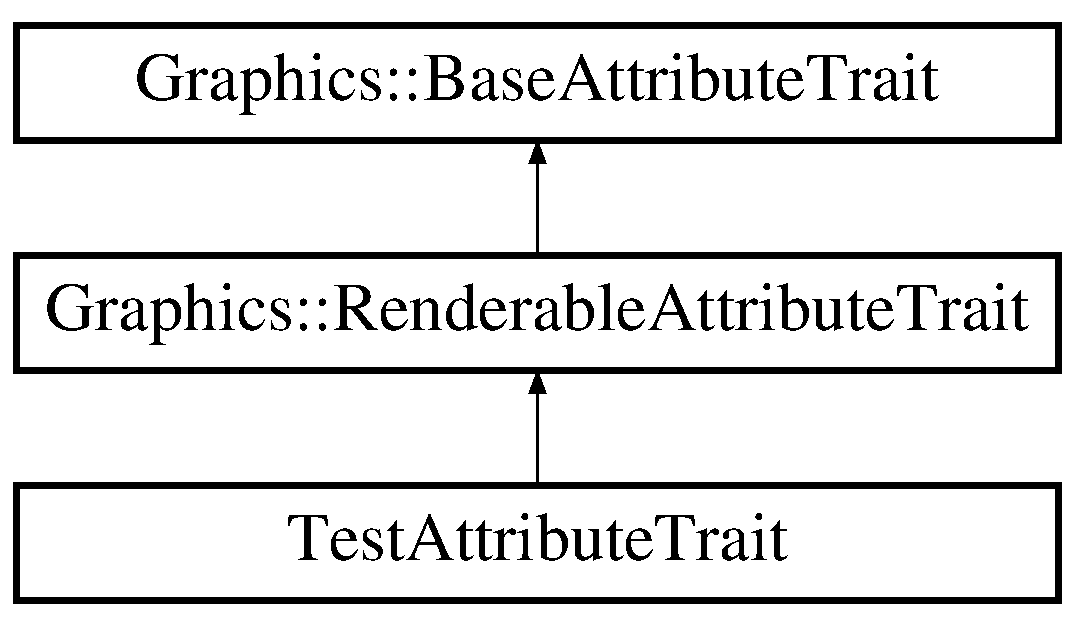
\includegraphics[height=3.000000cm]{class_graphics_1_1_renderable_attribute_trait}
\end{center}
\end{figure}
\subsection*{Public Member Functions}
\begin{DoxyCompactItemize}
\item 
\hyperlink{class_graphics_1_1_renderable_attribute_trait_afae7775a218a12c44a77c9d2190fccd3}{Renderable\+Attribute\+Trait} ()
\item 
virtual const std\+::map$<$ \hyperlink{class_graphics_1_1_vertex_data_a50e88236939dc2a3ec4df7aeb728620e}{Vertex\+Data\+::\+D\+A\+T\+A\+\_\+\+T\+Y\+P\+E}, unsigned int $>$ \hyperlink{class_graphics_1_1_renderable_attribute_trait_a44401f624ace1dc71220e7064db92465}{operator()} () const noexceptoverride
\end{DoxyCompactItemize}
\subsection*{Private Attributes}
\begin{DoxyCompactItemize}
\item 
std\+::map$<$ \hyperlink{class_graphics_1_1_vertex_data_a50e88236939dc2a3ec4df7aeb728620e}{Vertex\+Data\+::\+D\+A\+T\+A\+\_\+\+T\+Y\+P\+E}, unsigned int $>$ \hyperlink{class_graphics_1_1_renderable_attribute_trait_aa20fd62c99d1635eabe9a7fd73a67b32}{trait}
\end{DoxyCompactItemize}


\subsection{Constructor \& Destructor Documentation}
\hypertarget{class_graphics_1_1_renderable_attribute_trait_afae7775a218a12c44a77c9d2190fccd3}{}\index{Graphics\+::\+Renderable\+Attribute\+Trait@{Graphics\+::\+Renderable\+Attribute\+Trait}!Renderable\+Attribute\+Trait@{Renderable\+Attribute\+Trait}}
\index{Renderable\+Attribute\+Trait@{Renderable\+Attribute\+Trait}!Graphics\+::\+Renderable\+Attribute\+Trait@{Graphics\+::\+Renderable\+Attribute\+Trait}}
\subsubsection[{Renderable\+Attribute\+Trait}]{\setlength{\rightskip}{0pt plus 5cm}Graphics\+::\+Renderable\+Attribute\+Trait\+::\+Renderable\+Attribute\+Trait (
\begin{DoxyParamCaption}
{}
\end{DoxyParamCaption}
)\hspace{0.3cm}{\ttfamily [inline]}}\label{class_graphics_1_1_renderable_attribute_trait_afae7775a218a12c44a77c9d2190fccd3}


\subsection{Member Function Documentation}
\hypertarget{class_graphics_1_1_renderable_attribute_trait_a44401f624ace1dc71220e7064db92465}{}\index{Graphics\+::\+Renderable\+Attribute\+Trait@{Graphics\+::\+Renderable\+Attribute\+Trait}!operator()@{operator()}}
\index{operator()@{operator()}!Graphics\+::\+Renderable\+Attribute\+Trait@{Graphics\+::\+Renderable\+Attribute\+Trait}}
\subsubsection[{operator()}]{\setlength{\rightskip}{0pt plus 5cm}virtual const std\+::map$<${\bf Vertex\+Data\+::\+D\+A\+T\+A\+\_\+\+T\+Y\+P\+E}, unsigned int$>$ Graphics\+::\+Renderable\+Attribute\+Trait\+::operator() (
\begin{DoxyParamCaption}
{}
\end{DoxyParamCaption}
) const\hspace{0.3cm}{\ttfamily [inline]}, {\ttfamily [override]}, {\ttfamily [virtual]}, {\ttfamily [noexcept]}}\label{class_graphics_1_1_renderable_attribute_trait_a44401f624ace1dc71220e7064db92465}


Implements \hyperlink{class_graphics_1_1_base_attribute_trait_a7f43cabd619b64be1a0056e0fe568cf5}{Graphics\+::\+Base\+Attribute\+Trait}.



Reimplemented in \hyperlink{class_test_attribute_trait_af121ef5fbd5bcda4bbbc7fdadd5599c8}{Test\+Attribute\+Trait}.



\subsection{Member Data Documentation}
\hypertarget{class_graphics_1_1_renderable_attribute_trait_aa20fd62c99d1635eabe9a7fd73a67b32}{}\index{Graphics\+::\+Renderable\+Attribute\+Trait@{Graphics\+::\+Renderable\+Attribute\+Trait}!trait@{trait}}
\index{trait@{trait}!Graphics\+::\+Renderable\+Attribute\+Trait@{Graphics\+::\+Renderable\+Attribute\+Trait}}
\subsubsection[{trait}]{\setlength{\rightskip}{0pt plus 5cm}std\+::map$<${\bf Vertex\+Data\+::\+D\+A\+T\+A\+\_\+\+T\+Y\+P\+E}, unsigned int$>$ Graphics\+::\+Renderable\+Attribute\+Trait\+::trait\hspace{0.3cm}{\ttfamily [private]}}\label{class_graphics_1_1_renderable_attribute_trait_aa20fd62c99d1635eabe9a7fd73a67b32}


The documentation for this class was generated from the following file\+:\begin{DoxyCompactItemize}
\item 
src/graphics/\hyperlink{renderable__attribute__trait_8h}{renderable\+\_\+attribute\+\_\+trait.\+h}\end{DoxyCompactItemize}

\hypertarget{class_exceptions_1_1_renderable_not_initialized_exception}{}\section{Exceptions\+:\+:Renderable\+Not\+Initialized\+Exception Class Reference}
\label{class_exceptions_1_1_renderable_not_initialized_exception}\index{Exceptions\+::\+Renderable\+Not\+Initialized\+Exception@{Exceptions\+::\+Renderable\+Not\+Initialized\+Exception}}


{\ttfamily \#include $<$renderable\+\_\+not\+\_\+initialized\+\_\+exception.\+h$>$}

Inheritance diagram for Exceptions\+:\+:Renderable\+Not\+Initialized\+Exception\+:\begin{figure}[H]
\begin{center}
\leavevmode
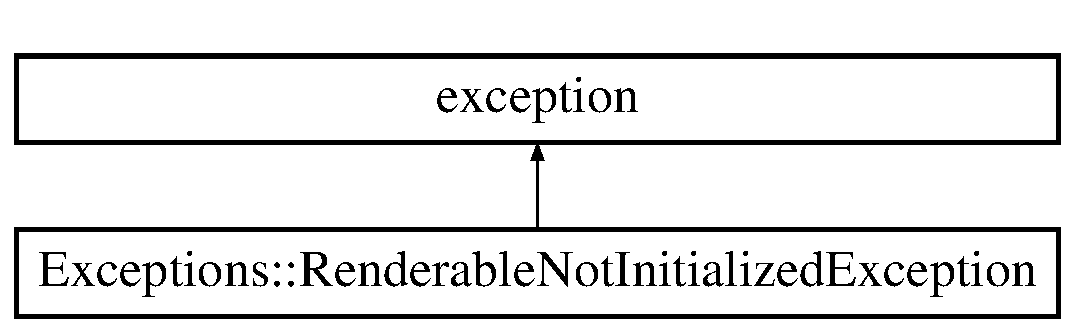
\includegraphics[height=2.000000cm]{class_exceptions_1_1_renderable_not_initialized_exception}
\end{center}
\end{figure}
\subsection*{Public Member Functions}
\begin{DoxyCompactItemize}
\item 
\hyperlink{class_exceptions_1_1_renderable_not_initialized_exception_a18c5b3c635950038831820df28b81bc5}{Renderable\+Not\+Initialized\+Exception} ()
\item 
virtual const char $\ast$ \hyperlink{class_exceptions_1_1_renderable_not_initialized_exception_a95b9337f6209c8df79b3120cd3e1ad5e}{what} () const   throw ()
\end{DoxyCompactItemize}


\subsection{Constructor \& Destructor Documentation}
\hypertarget{class_exceptions_1_1_renderable_not_initialized_exception_a18c5b3c635950038831820df28b81bc5}{}\index{Exceptions\+::\+Renderable\+Not\+Initialized\+Exception@{Exceptions\+::\+Renderable\+Not\+Initialized\+Exception}!Renderable\+Not\+Initialized\+Exception@{Renderable\+Not\+Initialized\+Exception}}
\index{Renderable\+Not\+Initialized\+Exception@{Renderable\+Not\+Initialized\+Exception}!Exceptions\+::\+Renderable\+Not\+Initialized\+Exception@{Exceptions\+::\+Renderable\+Not\+Initialized\+Exception}}
\subsubsection[{Renderable\+Not\+Initialized\+Exception}]{\setlength{\rightskip}{0pt plus 5cm}Exceptions\+::\+Renderable\+Not\+Initialized\+Exception\+::\+Renderable\+Not\+Initialized\+Exception (
\begin{DoxyParamCaption}
{}
\end{DoxyParamCaption}
)\hspace{0.3cm}{\ttfamily [inline]}}\label{class_exceptions_1_1_renderable_not_initialized_exception_a18c5b3c635950038831820df28b81bc5}


\subsection{Member Function Documentation}
\hypertarget{class_exceptions_1_1_renderable_not_initialized_exception_a95b9337f6209c8df79b3120cd3e1ad5e}{}\index{Exceptions\+::\+Renderable\+Not\+Initialized\+Exception@{Exceptions\+::\+Renderable\+Not\+Initialized\+Exception}!what@{what}}
\index{what@{what}!Exceptions\+::\+Renderable\+Not\+Initialized\+Exception@{Exceptions\+::\+Renderable\+Not\+Initialized\+Exception}}
\subsubsection[{what}]{\setlength{\rightskip}{0pt plus 5cm}virtual const char$\ast$ Exceptions\+::\+Renderable\+Not\+Initialized\+Exception\+::what (
\begin{DoxyParamCaption}
{}
\end{DoxyParamCaption}
) const throw  ) \hspace{0.3cm}{\ttfamily [inline]}, {\ttfamily [virtual]}}\label{class_exceptions_1_1_renderable_not_initialized_exception_a95b9337f6209c8df79b3120cd3e1ad5e}


The documentation for this class was generated from the following file\+:\begin{DoxyCompactItemize}
\item 
src/exceptions/\hyperlink{renderable__not__initialized__exception_8h}{renderable\+\_\+not\+\_\+initialized\+\_\+exception.\+h}\end{DoxyCompactItemize}

\hypertarget{class_graphics_1_1_shader}{}\section{Graphics\+:\+:Shader Class Reference}
\label{class_graphics_1_1_shader}\index{Graphics\+::\+Shader@{Graphics\+::\+Shader}}


{\ttfamily \#include $<$shader.\+h$>$}

\subsection*{Public Member Functions}
\begin{DoxyCompactItemize}
\item 
\hyperlink{class_graphics_1_1_shader_a8160ac75561d286213ec65ec30d9eeb0}{Shader} ()=delete
\item 
\hyperlink{class_graphics_1_1_shader_aef598fb3433acea1aff5e57499d08fed}{Shader} (const unsigned int vertex\+\_\+program, const unsigned int fragment\+\_\+program, const unsigned int geometry\+\_\+program=0)
\item 
const unsigned int \hyperlink{class_graphics_1_1_shader_a8310ca4e5e8dba64d1ad3636bada078b}{get\+Handle} () const noexcept
\item 
void \hyperlink{class_graphics_1_1_shader_a564d1802984fc0501f33528e8fe5aad3}{use\+Program} () const 
\item 
{\footnotesize template$<$class T $>$ }\\void \hyperlink{class_graphics_1_1_shader_a78f6ffc5d8fc4d3eee3189dae6e8434e}{set\+Uniform} (const std\+::string \&name, const T \&value)
\item 
{\footnotesize template$<$$>$ }\\void \hyperlink{class_graphics_1_1_shader_ae87e687bdc5b41e7162a3fd17cbe4b8c}{set\+Uniform} (const std\+::string \&name, const float \&data)
\item 
{\footnotesize template$<$$>$ }\\void \hyperlink{class_graphics_1_1_shader_a053a18f48bf33e427ae912e420f41300}{set\+Uniform} (const std\+::string \&name, const int \&data)
\item 
{\footnotesize template$<$$>$ }\\void \hyperlink{class_graphics_1_1_shader_abe8990b3404bfedef5a29d7557bf2ad8}{set\+Uniform} (const std\+::string \&name, const unsigned int \&data)
\item 
{\footnotesize template$<$$>$ }\\void \hyperlink{class_graphics_1_1_shader_a70df2013998b9cb0efce4bb3177c9599}{set\+Uniform} (const std\+::string \&name, const bool \&data)
\end{DoxyCompactItemize}
\subsection*{Private Attributes}
\begin{DoxyCompactItemize}
\item 
unsigned int \hyperlink{class_graphics_1_1_shader_a8e40ca5eb9880e84c29366dbe626c081}{program\+\_\+object}
\item 
std\+::map$<$ std\+::string, int $>$ \hyperlink{class_graphics_1_1_shader_a71b17a1ca67b9315b0aa44bb984a8617}{name\+\_\+to\+\_\+location}
\item 
std\+::map$<$ std\+::string, G\+Lenum $>$ \hyperlink{class_graphics_1_1_shader_a591f5dbbfbb6a851fb9bd88a91c17135}{name\+\_\+to\+\_\+type}
\end{DoxyCompactItemize}


\subsection{Constructor \& Destructor Documentation}
\hypertarget{class_graphics_1_1_shader_a8160ac75561d286213ec65ec30d9eeb0}{}\index{Graphics\+::\+Shader@{Graphics\+::\+Shader}!Shader@{Shader}}
\index{Shader@{Shader}!Graphics\+::\+Shader@{Graphics\+::\+Shader}}
\subsubsection[{Shader}]{\setlength{\rightskip}{0pt plus 5cm}Graphics\+::\+Shader\+::\+Shader (
\begin{DoxyParamCaption}
{}
\end{DoxyParamCaption}
)\hspace{0.3cm}{\ttfamily [delete]}}\label{class_graphics_1_1_shader_a8160ac75561d286213ec65ec30d9eeb0}
\hypertarget{class_graphics_1_1_shader_aef598fb3433acea1aff5e57499d08fed}{}\index{Graphics\+::\+Shader@{Graphics\+::\+Shader}!Shader@{Shader}}
\index{Shader@{Shader}!Graphics\+::\+Shader@{Graphics\+::\+Shader}}
\subsubsection[{Shader}]{\setlength{\rightskip}{0pt plus 5cm}Graphics\+::\+Shader\+::\+Shader (
\begin{DoxyParamCaption}
\item[{const unsigned int}]{vertex\+\_\+program, }
\item[{const unsigned int}]{fragment\+\_\+program, }
\item[{const unsigned int}]{geometry\+\_\+program = {\ttfamily 0}}
\end{DoxyParamCaption}
)}\label{class_graphics_1_1_shader_aef598fb3433acea1aff5e57499d08fed}


\subsection{Member Function Documentation}
\hypertarget{class_graphics_1_1_shader_a8310ca4e5e8dba64d1ad3636bada078b}{}\index{Graphics\+::\+Shader@{Graphics\+::\+Shader}!get\+Handle@{get\+Handle}}
\index{get\+Handle@{get\+Handle}!Graphics\+::\+Shader@{Graphics\+::\+Shader}}
\subsubsection[{get\+Handle}]{\setlength{\rightskip}{0pt plus 5cm}const unsigned int Graphics\+::\+Shader\+::get\+Handle (
\begin{DoxyParamCaption}
{}
\end{DoxyParamCaption}
) const\hspace{0.3cm}{\ttfamily [noexcept]}}\label{class_graphics_1_1_shader_a8310ca4e5e8dba64d1ad3636bada078b}
\hypertarget{class_graphics_1_1_shader_a78f6ffc5d8fc4d3eee3189dae6e8434e}{}\index{Graphics\+::\+Shader@{Graphics\+::\+Shader}!set\+Uniform@{set\+Uniform}}
\index{set\+Uniform@{set\+Uniform}!Graphics\+::\+Shader@{Graphics\+::\+Shader}}
\subsubsection[{set\+Uniform}]{\setlength{\rightskip}{0pt plus 5cm}template$<$class T $>$ void Graphics\+::\+Shader\+::set\+Uniform (
\begin{DoxyParamCaption}
\item[{const std\+::string \&}]{name, }
\item[{const T \&}]{value}
\end{DoxyParamCaption}
)}\label{class_graphics_1_1_shader_a78f6ffc5d8fc4d3eee3189dae6e8434e}
\hypertarget{class_graphics_1_1_shader_ae87e687bdc5b41e7162a3fd17cbe4b8c}{}\index{Graphics\+::\+Shader@{Graphics\+::\+Shader}!set\+Uniform@{set\+Uniform}}
\index{set\+Uniform@{set\+Uniform}!Graphics\+::\+Shader@{Graphics\+::\+Shader}}
\subsubsection[{set\+Uniform}]{\setlength{\rightskip}{0pt plus 5cm}template$<$$>$ void Graphics\+::\+Shader\+::set\+Uniform (
\begin{DoxyParamCaption}
\item[{const std\+::string \&}]{name, }
\item[{const float \&}]{data}
\end{DoxyParamCaption}
)}\label{class_graphics_1_1_shader_ae87e687bdc5b41e7162a3fd17cbe4b8c}
\hypertarget{class_graphics_1_1_shader_a053a18f48bf33e427ae912e420f41300}{}\index{Graphics\+::\+Shader@{Graphics\+::\+Shader}!set\+Uniform@{set\+Uniform}}
\index{set\+Uniform@{set\+Uniform}!Graphics\+::\+Shader@{Graphics\+::\+Shader}}
\subsubsection[{set\+Uniform}]{\setlength{\rightskip}{0pt plus 5cm}template$<$$>$ void Graphics\+::\+Shader\+::set\+Uniform (
\begin{DoxyParamCaption}
\item[{const std\+::string \&}]{name, }
\item[{const int \&}]{data}
\end{DoxyParamCaption}
)}\label{class_graphics_1_1_shader_a053a18f48bf33e427ae912e420f41300}
\hypertarget{class_graphics_1_1_shader_abe8990b3404bfedef5a29d7557bf2ad8}{}\index{Graphics\+::\+Shader@{Graphics\+::\+Shader}!set\+Uniform@{set\+Uniform}}
\index{set\+Uniform@{set\+Uniform}!Graphics\+::\+Shader@{Graphics\+::\+Shader}}
\subsubsection[{set\+Uniform}]{\setlength{\rightskip}{0pt plus 5cm}template$<$$>$ void Graphics\+::\+Shader\+::set\+Uniform (
\begin{DoxyParamCaption}
\item[{const std\+::string \&}]{name, }
\item[{const unsigned int \&}]{data}
\end{DoxyParamCaption}
)}\label{class_graphics_1_1_shader_abe8990b3404bfedef5a29d7557bf2ad8}
\hypertarget{class_graphics_1_1_shader_a70df2013998b9cb0efce4bb3177c9599}{}\index{Graphics\+::\+Shader@{Graphics\+::\+Shader}!set\+Uniform@{set\+Uniform}}
\index{set\+Uniform@{set\+Uniform}!Graphics\+::\+Shader@{Graphics\+::\+Shader}}
\subsubsection[{set\+Uniform}]{\setlength{\rightskip}{0pt plus 5cm}template$<$$>$ void Graphics\+::\+Shader\+::set\+Uniform (
\begin{DoxyParamCaption}
\item[{const std\+::string \&}]{name, }
\item[{const bool \&}]{data}
\end{DoxyParamCaption}
)}\label{class_graphics_1_1_shader_a70df2013998b9cb0efce4bb3177c9599}
\hypertarget{class_graphics_1_1_shader_a564d1802984fc0501f33528e8fe5aad3}{}\index{Graphics\+::\+Shader@{Graphics\+::\+Shader}!use\+Program@{use\+Program}}
\index{use\+Program@{use\+Program}!Graphics\+::\+Shader@{Graphics\+::\+Shader}}
\subsubsection[{use\+Program}]{\setlength{\rightskip}{0pt plus 5cm}void Graphics\+::\+Shader\+::use\+Program (
\begin{DoxyParamCaption}
{}
\end{DoxyParamCaption}
) const}\label{class_graphics_1_1_shader_a564d1802984fc0501f33528e8fe5aad3}


\subsection{Member Data Documentation}
\hypertarget{class_graphics_1_1_shader_a71b17a1ca67b9315b0aa44bb984a8617}{}\index{Graphics\+::\+Shader@{Graphics\+::\+Shader}!name\+\_\+to\+\_\+location@{name\+\_\+to\+\_\+location}}
\index{name\+\_\+to\+\_\+location@{name\+\_\+to\+\_\+location}!Graphics\+::\+Shader@{Graphics\+::\+Shader}}
\subsubsection[{name\+\_\+to\+\_\+location}]{\setlength{\rightskip}{0pt plus 5cm}std\+::map$<$std\+::string, int$>$ Graphics\+::\+Shader\+::name\+\_\+to\+\_\+location\hspace{0.3cm}{\ttfamily [private]}}\label{class_graphics_1_1_shader_a71b17a1ca67b9315b0aa44bb984a8617}
\hypertarget{class_graphics_1_1_shader_a591f5dbbfbb6a851fb9bd88a91c17135}{}\index{Graphics\+::\+Shader@{Graphics\+::\+Shader}!name\+\_\+to\+\_\+type@{name\+\_\+to\+\_\+type}}
\index{name\+\_\+to\+\_\+type@{name\+\_\+to\+\_\+type}!Graphics\+::\+Shader@{Graphics\+::\+Shader}}
\subsubsection[{name\+\_\+to\+\_\+type}]{\setlength{\rightskip}{0pt plus 5cm}std\+::map$<$std\+::string, G\+Lenum$>$ Graphics\+::\+Shader\+::name\+\_\+to\+\_\+type\hspace{0.3cm}{\ttfamily [private]}}\label{class_graphics_1_1_shader_a591f5dbbfbb6a851fb9bd88a91c17135}
\hypertarget{class_graphics_1_1_shader_a8e40ca5eb9880e84c29366dbe626c081}{}\index{Graphics\+::\+Shader@{Graphics\+::\+Shader}!program\+\_\+object@{program\+\_\+object}}
\index{program\+\_\+object@{program\+\_\+object}!Graphics\+::\+Shader@{Graphics\+::\+Shader}}
\subsubsection[{program\+\_\+object}]{\setlength{\rightskip}{0pt plus 5cm}unsigned int Graphics\+::\+Shader\+::program\+\_\+object\hspace{0.3cm}{\ttfamily [private]}}\label{class_graphics_1_1_shader_a8e40ca5eb9880e84c29366dbe626c081}


The documentation for this class was generated from the following files\+:\begin{DoxyCompactItemize}
\item 
src/graphics/\hyperlink{shader_8h}{shader.\+h}\item 
src/graphics/\hyperlink{shader_8cpp}{shader.\+cpp}\end{DoxyCompactItemize}

\hypertarget{class_graphics_1_1_shader_manager}{}\section{Graphics\+:\+:Shader\+Manager Class Reference}
\label{class_graphics_1_1_shader_manager}\index{Graphics\+::\+Shader\+Manager@{Graphics\+::\+Shader\+Manager}}


{\ttfamily \#include $<$shader\+\_\+manager.\+h$>$}

\subsection*{Public Member Functions}
\begin{DoxyCompactItemize}
\item 
\hyperlink{class_graphics_1_1_shader_manager_ac5f14e07d3b7bffa4b4cf63d9c4fb3a7}{Shader\+Manager} ()
\item 
\hyperlink{class_graphics_1_1_shader_manager_a1846632f26cfcb4907844716f23e0540}{$\sim$\+Shader\+Manager} ()
\item 
const bool \hyperlink{class_graphics_1_1_shader_manager_a29234192f964ad1d9da812e8ceab008f}{load\+Shader} (const std\+::string \&name, const bool geometry\+\_\+shader=false)
\item 
const bool \hyperlink{class_graphics_1_1_shader_manager_a0cd014938152e36fd81717dadd7e390a}{load\+Shader} (const std\+::string \&name, const std\+::string \&vertex\+\_\+filename, const std\+::string \&fragment\+\_\+filename, const std\+::string \&geometry\+\_\+filename)
\item 
const std\+::shared\+\_\+ptr$<$ \hyperlink{class_graphics_1_1_shader}{Shader} $>$ \hyperlink{class_graphics_1_1_shader_manager_a4a3c0f369be06a34a8e44ad8a41862a4}{operator\mbox{[}$\,$\mbox{]}} (const std\+::string \&name) const 
\item 
const std\+::shared\+\_\+ptr$<$ \hyperlink{class_graphics_1_1_shader}{Shader} $>$ \hyperlink{class_graphics_1_1_shader_manager_a8c82c5f8d73dbb9ec3038b2db71add41}{get\+Shader} (const std\+::string \&name) const 
\end{DoxyCompactItemize}
\subsection*{Static Public Attributes}
\begin{DoxyCompactItemize}
\item 
static char const $\ast$ \hyperlink{class_graphics_1_1_shader_manager_abb954de5b5b6bc56d568e20b478f0712}{V\+E\+R\+T\+E\+X\+\_\+\+E\+X\+T\+E\+N\+S\+I\+O\+N} = \char`\"{}.vert\char`\"{}
\item 
static char const $\ast$ \hyperlink{class_graphics_1_1_shader_manager_aa3ad06b558229fe4d4d4ebbabfe9ca48}{F\+R\+A\+G\+M\+E\+N\+T\+\_\+\+E\+X\+T\+E\+N\+S\+I\+O\+N} = \char`\"{}.frag\char`\"{}
\item 
static char const $\ast$ \hyperlink{class_graphics_1_1_shader_manager_a66cf54024f2f1e51db6f5afccbcba67e}{G\+E\+O\+M\+E\+T\+R\+Y\+\_\+\+E\+X\+T\+E\+N\+S\+I\+O\+N} = \char`\"{}.geom\char`\"{}
\item 
static char const $\ast$ \hyperlink{class_graphics_1_1_shader_manager_ad3cef3602a2a0205064bdff0ac9437a8}{S\+H\+A\+D\+E\+R\+\_\+\+D\+I\+R\+E\+C\+T\+O\+R\+Y} = \char`\"{}./shaders/\char`\"{}
\end{DoxyCompactItemize}
\subsection*{Private Attributes}
\begin{DoxyCompactItemize}
\item 
std\+::map$<$ std\+::string, std\+::shared\+\_\+ptr$<$ \hyperlink{class_graphics_1_1_shader}{Shader} $>$ $>$ \hyperlink{class_graphics_1_1_shader_manager_a5cada9e001d0b2ead2bfb7a0ef37be66}{shaders\+\_\+to\+\_\+names}
\end{DoxyCompactItemize}


\subsection{Constructor \& Destructor Documentation}
\hypertarget{class_graphics_1_1_shader_manager_ac5f14e07d3b7bffa4b4cf63d9c4fb3a7}{}\index{Graphics\+::\+Shader\+Manager@{Graphics\+::\+Shader\+Manager}!Shader\+Manager@{Shader\+Manager}}
\index{Shader\+Manager@{Shader\+Manager}!Graphics\+::\+Shader\+Manager@{Graphics\+::\+Shader\+Manager}}
\subsubsection[{Shader\+Manager}]{\setlength{\rightskip}{0pt plus 5cm}Graphics\+::\+Shader\+Manager\+::\+Shader\+Manager (
\begin{DoxyParamCaption}
{}
\end{DoxyParamCaption}
)}\label{class_graphics_1_1_shader_manager_ac5f14e07d3b7bffa4b4cf63d9c4fb3a7}
\hypertarget{class_graphics_1_1_shader_manager_a1846632f26cfcb4907844716f23e0540}{}\index{Graphics\+::\+Shader\+Manager@{Graphics\+::\+Shader\+Manager}!````~Shader\+Manager@{$\sim$\+Shader\+Manager}}
\index{````~Shader\+Manager@{$\sim$\+Shader\+Manager}!Graphics\+::\+Shader\+Manager@{Graphics\+::\+Shader\+Manager}}
\subsubsection[{$\sim$\+Shader\+Manager}]{\setlength{\rightskip}{0pt plus 5cm}Graphics\+::\+Shader\+Manager\+::$\sim$\+Shader\+Manager (
\begin{DoxyParamCaption}
{}
\end{DoxyParamCaption}
)}\label{class_graphics_1_1_shader_manager_a1846632f26cfcb4907844716f23e0540}


\subsection{Member Function Documentation}
\hypertarget{class_graphics_1_1_shader_manager_a8c82c5f8d73dbb9ec3038b2db71add41}{}\index{Graphics\+::\+Shader\+Manager@{Graphics\+::\+Shader\+Manager}!get\+Shader@{get\+Shader}}
\index{get\+Shader@{get\+Shader}!Graphics\+::\+Shader\+Manager@{Graphics\+::\+Shader\+Manager}}
\subsubsection[{get\+Shader}]{\setlength{\rightskip}{0pt plus 5cm}const std\+::shared\+\_\+ptr$<$ {\bf Shader} $>$ Graphics\+::\+Shader\+Manager\+::get\+Shader (
\begin{DoxyParamCaption}
\item[{const std\+::string \&}]{name}
\end{DoxyParamCaption}
) const}\label{class_graphics_1_1_shader_manager_a8c82c5f8d73dbb9ec3038b2db71add41}
\hypertarget{class_graphics_1_1_shader_manager_a29234192f964ad1d9da812e8ceab008f}{}\index{Graphics\+::\+Shader\+Manager@{Graphics\+::\+Shader\+Manager}!load\+Shader@{load\+Shader}}
\index{load\+Shader@{load\+Shader}!Graphics\+::\+Shader\+Manager@{Graphics\+::\+Shader\+Manager}}
\subsubsection[{load\+Shader}]{\setlength{\rightskip}{0pt plus 5cm}const bool Graphics\+::\+Shader\+Manager\+::load\+Shader (
\begin{DoxyParamCaption}
\item[{const std\+::string \&}]{name, }
\item[{const bool}]{geometry\+\_\+shader = {\ttfamily false}}
\end{DoxyParamCaption}
)}\label{class_graphics_1_1_shader_manager_a29234192f964ad1d9da812e8ceab008f}
\hypertarget{class_graphics_1_1_shader_manager_a0cd014938152e36fd81717dadd7e390a}{}\index{Graphics\+::\+Shader\+Manager@{Graphics\+::\+Shader\+Manager}!load\+Shader@{load\+Shader}}
\index{load\+Shader@{load\+Shader}!Graphics\+::\+Shader\+Manager@{Graphics\+::\+Shader\+Manager}}
\subsubsection[{load\+Shader}]{\setlength{\rightskip}{0pt plus 5cm}const bool Graphics\+::\+Shader\+Manager\+::load\+Shader (
\begin{DoxyParamCaption}
\item[{const std\+::string \&}]{name, }
\item[{const std\+::string \&}]{vertex\+\_\+filename, }
\item[{const std\+::string \&}]{fragment\+\_\+filename, }
\item[{const std\+::string \&}]{geometry\+\_\+filename}
\end{DoxyParamCaption}
)}\label{class_graphics_1_1_shader_manager_a0cd014938152e36fd81717dadd7e390a}
\hypertarget{class_graphics_1_1_shader_manager_a4a3c0f369be06a34a8e44ad8a41862a4}{}\index{Graphics\+::\+Shader\+Manager@{Graphics\+::\+Shader\+Manager}!operator\mbox{[}$\,$\mbox{]}@{operator[]}}
\index{operator\mbox{[}$\,$\mbox{]}@{operator[]}!Graphics\+::\+Shader\+Manager@{Graphics\+::\+Shader\+Manager}}
\subsubsection[{operator[]}]{\setlength{\rightskip}{0pt plus 5cm}const std\+::shared\+\_\+ptr$<$ {\bf Shader} $>$ Graphics\+::\+Shader\+Manager\+::operator\mbox{[}$\,$\mbox{]} (
\begin{DoxyParamCaption}
\item[{const std\+::string \&}]{name}
\end{DoxyParamCaption}
) const}\label{class_graphics_1_1_shader_manager_a4a3c0f369be06a34a8e44ad8a41862a4}


\subsection{Member Data Documentation}
\hypertarget{class_graphics_1_1_shader_manager_aa3ad06b558229fe4d4d4ebbabfe9ca48}{}\index{Graphics\+::\+Shader\+Manager@{Graphics\+::\+Shader\+Manager}!F\+R\+A\+G\+M\+E\+N\+T\+\_\+\+E\+X\+T\+E\+N\+S\+I\+O\+N@{F\+R\+A\+G\+M\+E\+N\+T\+\_\+\+E\+X\+T\+E\+N\+S\+I\+O\+N}}
\index{F\+R\+A\+G\+M\+E\+N\+T\+\_\+\+E\+X\+T\+E\+N\+S\+I\+O\+N@{F\+R\+A\+G\+M\+E\+N\+T\+\_\+\+E\+X\+T\+E\+N\+S\+I\+O\+N}!Graphics\+::\+Shader\+Manager@{Graphics\+::\+Shader\+Manager}}
\subsubsection[{F\+R\+A\+G\+M\+E\+N\+T\+\_\+\+E\+X\+T\+E\+N\+S\+I\+O\+N}]{\setlength{\rightskip}{0pt plus 5cm}char const $\ast$ Graphics\+::\+Shader\+Manager\+::\+F\+R\+A\+G\+M\+E\+N\+T\+\_\+\+E\+X\+T\+E\+N\+S\+I\+O\+N = \char`\"{}.frag\char`\"{}\hspace{0.3cm}{\ttfamily [static]}}\label{class_graphics_1_1_shader_manager_aa3ad06b558229fe4d4d4ebbabfe9ca48}
\hypertarget{class_graphics_1_1_shader_manager_a66cf54024f2f1e51db6f5afccbcba67e}{}\index{Graphics\+::\+Shader\+Manager@{Graphics\+::\+Shader\+Manager}!G\+E\+O\+M\+E\+T\+R\+Y\+\_\+\+E\+X\+T\+E\+N\+S\+I\+O\+N@{G\+E\+O\+M\+E\+T\+R\+Y\+\_\+\+E\+X\+T\+E\+N\+S\+I\+O\+N}}
\index{G\+E\+O\+M\+E\+T\+R\+Y\+\_\+\+E\+X\+T\+E\+N\+S\+I\+O\+N@{G\+E\+O\+M\+E\+T\+R\+Y\+\_\+\+E\+X\+T\+E\+N\+S\+I\+O\+N}!Graphics\+::\+Shader\+Manager@{Graphics\+::\+Shader\+Manager}}
\subsubsection[{G\+E\+O\+M\+E\+T\+R\+Y\+\_\+\+E\+X\+T\+E\+N\+S\+I\+O\+N}]{\setlength{\rightskip}{0pt plus 5cm}char const $\ast$ Graphics\+::\+Shader\+Manager\+::\+G\+E\+O\+M\+E\+T\+R\+Y\+\_\+\+E\+X\+T\+E\+N\+S\+I\+O\+N = \char`\"{}.geom\char`\"{}\hspace{0.3cm}{\ttfamily [static]}}\label{class_graphics_1_1_shader_manager_a66cf54024f2f1e51db6f5afccbcba67e}
\hypertarget{class_graphics_1_1_shader_manager_ad3cef3602a2a0205064bdff0ac9437a8}{}\index{Graphics\+::\+Shader\+Manager@{Graphics\+::\+Shader\+Manager}!S\+H\+A\+D\+E\+R\+\_\+\+D\+I\+R\+E\+C\+T\+O\+R\+Y@{S\+H\+A\+D\+E\+R\+\_\+\+D\+I\+R\+E\+C\+T\+O\+R\+Y}}
\index{S\+H\+A\+D\+E\+R\+\_\+\+D\+I\+R\+E\+C\+T\+O\+R\+Y@{S\+H\+A\+D\+E\+R\+\_\+\+D\+I\+R\+E\+C\+T\+O\+R\+Y}!Graphics\+::\+Shader\+Manager@{Graphics\+::\+Shader\+Manager}}
\subsubsection[{S\+H\+A\+D\+E\+R\+\_\+\+D\+I\+R\+E\+C\+T\+O\+R\+Y}]{\setlength{\rightskip}{0pt plus 5cm}char const $\ast$ Graphics\+::\+Shader\+Manager\+::\+S\+H\+A\+D\+E\+R\+\_\+\+D\+I\+R\+E\+C\+T\+O\+R\+Y = \char`\"{}./shaders/\char`\"{}\hspace{0.3cm}{\ttfamily [static]}}\label{class_graphics_1_1_shader_manager_ad3cef3602a2a0205064bdff0ac9437a8}
\hypertarget{class_graphics_1_1_shader_manager_a5cada9e001d0b2ead2bfb7a0ef37be66}{}\index{Graphics\+::\+Shader\+Manager@{Graphics\+::\+Shader\+Manager}!shaders\+\_\+to\+\_\+names@{shaders\+\_\+to\+\_\+names}}
\index{shaders\+\_\+to\+\_\+names@{shaders\+\_\+to\+\_\+names}!Graphics\+::\+Shader\+Manager@{Graphics\+::\+Shader\+Manager}}
\subsubsection[{shaders\+\_\+to\+\_\+names}]{\setlength{\rightskip}{0pt plus 5cm}std\+::map$<$std\+::string, std\+::shared\+\_\+ptr$<${\bf Shader}$>$ $>$ Graphics\+::\+Shader\+Manager\+::shaders\+\_\+to\+\_\+names\hspace{0.3cm}{\ttfamily [private]}}\label{class_graphics_1_1_shader_manager_a5cada9e001d0b2ead2bfb7a0ef37be66}
\hypertarget{class_graphics_1_1_shader_manager_abb954de5b5b6bc56d568e20b478f0712}{}\index{Graphics\+::\+Shader\+Manager@{Graphics\+::\+Shader\+Manager}!V\+E\+R\+T\+E\+X\+\_\+\+E\+X\+T\+E\+N\+S\+I\+O\+N@{V\+E\+R\+T\+E\+X\+\_\+\+E\+X\+T\+E\+N\+S\+I\+O\+N}}
\index{V\+E\+R\+T\+E\+X\+\_\+\+E\+X\+T\+E\+N\+S\+I\+O\+N@{V\+E\+R\+T\+E\+X\+\_\+\+E\+X\+T\+E\+N\+S\+I\+O\+N}!Graphics\+::\+Shader\+Manager@{Graphics\+::\+Shader\+Manager}}
\subsubsection[{V\+E\+R\+T\+E\+X\+\_\+\+E\+X\+T\+E\+N\+S\+I\+O\+N}]{\setlength{\rightskip}{0pt plus 5cm}char const $\ast$ Graphics\+::\+Shader\+Manager\+::\+V\+E\+R\+T\+E\+X\+\_\+\+E\+X\+T\+E\+N\+S\+I\+O\+N = \char`\"{}.vert\char`\"{}\hspace{0.3cm}{\ttfamily [static]}}\label{class_graphics_1_1_shader_manager_abb954de5b5b6bc56d568e20b478f0712}


The documentation for this class was generated from the following files\+:\begin{DoxyCompactItemize}
\item 
src/graphics/\hyperlink{shader__manager_8h}{shader\+\_\+manager.\+h}\item 
src/graphics/\hyperlink{shader__manager_8cpp}{shader\+\_\+manager.\+cpp}\end{DoxyCompactItemize}

\hypertarget{class_exceptions_1_1_system_already_initialized_exception}{}\section{Exceptions\+:\+:System\+Already\+Initialized\+Exception Class Reference}
\label{class_exceptions_1_1_system_already_initialized_exception}\index{Exceptions\+::\+System\+Already\+Initialized\+Exception@{Exceptions\+::\+System\+Already\+Initialized\+Exception}}


{\ttfamily \#include $<$system\+\_\+already\+\_\+initialized\+\_\+exception.\+h$>$}

Inheritance diagram for Exceptions\+:\+:System\+Already\+Initialized\+Exception\+:\begin{figure}[H]
\begin{center}
\leavevmode
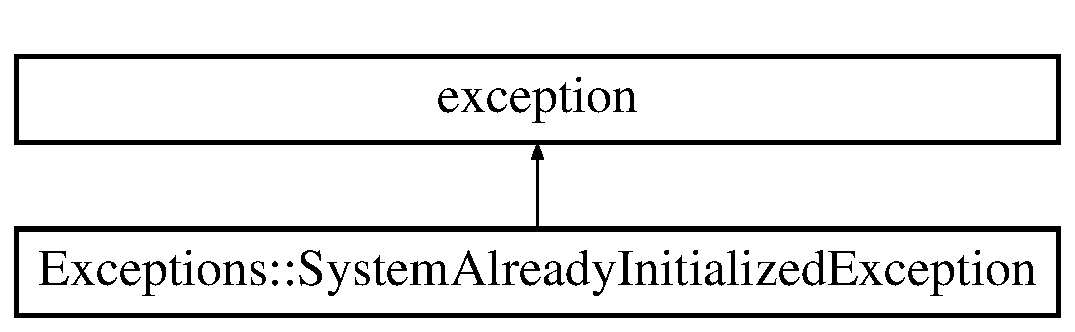
\includegraphics[height=2.000000cm]{class_exceptions_1_1_system_already_initialized_exception}
\end{center}
\end{figure}
\subsection*{Public Member Functions}
\begin{DoxyCompactItemize}
\item 
\hyperlink{class_exceptions_1_1_system_already_initialized_exception_a2f92ee1627417086ca29f3d58a8be520}{System\+Already\+Initialized\+Exception} (std\+::string \hyperlink{class_exceptions_1_1_system_already_initialized_exception_a858d81e072cf8a6a06a4fa506700fb32}{system\+\_\+name})
\item 
virtual const char $\ast$ \hyperlink{class_exceptions_1_1_system_already_initialized_exception_a28077450404b8dd5c89a348bc19ffa19}{what} () const   throw ()
\end{DoxyCompactItemize}
\subsection*{Private Attributes}
\begin{DoxyCompactItemize}
\item 
std\+::string \hyperlink{class_exceptions_1_1_system_already_initialized_exception_a858d81e072cf8a6a06a4fa506700fb32}{system\+\_\+name}
\end{DoxyCompactItemize}


\subsection{Constructor \& Destructor Documentation}
\hypertarget{class_exceptions_1_1_system_already_initialized_exception_a2f92ee1627417086ca29f3d58a8be520}{}\index{Exceptions\+::\+System\+Already\+Initialized\+Exception@{Exceptions\+::\+System\+Already\+Initialized\+Exception}!System\+Already\+Initialized\+Exception@{System\+Already\+Initialized\+Exception}}
\index{System\+Already\+Initialized\+Exception@{System\+Already\+Initialized\+Exception}!Exceptions\+::\+System\+Already\+Initialized\+Exception@{Exceptions\+::\+System\+Already\+Initialized\+Exception}}
\subsubsection[{System\+Already\+Initialized\+Exception}]{\setlength{\rightskip}{0pt plus 5cm}Exceptions\+::\+System\+Already\+Initialized\+Exception\+::\+System\+Already\+Initialized\+Exception (
\begin{DoxyParamCaption}
\item[{std\+::string}]{system\+\_\+name}
\end{DoxyParamCaption}
)\hspace{0.3cm}{\ttfamily [inline]}}\label{class_exceptions_1_1_system_already_initialized_exception_a2f92ee1627417086ca29f3d58a8be520}


\subsection{Member Function Documentation}
\hypertarget{class_exceptions_1_1_system_already_initialized_exception_a28077450404b8dd5c89a348bc19ffa19}{}\index{Exceptions\+::\+System\+Already\+Initialized\+Exception@{Exceptions\+::\+System\+Already\+Initialized\+Exception}!what@{what}}
\index{what@{what}!Exceptions\+::\+System\+Already\+Initialized\+Exception@{Exceptions\+::\+System\+Already\+Initialized\+Exception}}
\subsubsection[{what}]{\setlength{\rightskip}{0pt plus 5cm}virtual const char$\ast$ Exceptions\+::\+System\+Already\+Initialized\+Exception\+::what (
\begin{DoxyParamCaption}
{}
\end{DoxyParamCaption}
) const throw  ) \hspace{0.3cm}{\ttfamily [inline]}, {\ttfamily [virtual]}}\label{class_exceptions_1_1_system_already_initialized_exception_a28077450404b8dd5c89a348bc19ffa19}


\subsection{Member Data Documentation}
\hypertarget{class_exceptions_1_1_system_already_initialized_exception_a858d81e072cf8a6a06a4fa506700fb32}{}\index{Exceptions\+::\+System\+Already\+Initialized\+Exception@{Exceptions\+::\+System\+Already\+Initialized\+Exception}!system\+\_\+name@{system\+\_\+name}}
\index{system\+\_\+name@{system\+\_\+name}!Exceptions\+::\+System\+Already\+Initialized\+Exception@{Exceptions\+::\+System\+Already\+Initialized\+Exception}}
\subsubsection[{system\+\_\+name}]{\setlength{\rightskip}{0pt plus 5cm}std\+::string Exceptions\+::\+System\+Already\+Initialized\+Exception\+::system\+\_\+name\hspace{0.3cm}{\ttfamily [private]}}\label{class_exceptions_1_1_system_already_initialized_exception_a858d81e072cf8a6a06a4fa506700fb32}


The documentation for this class was generated from the following file\+:\begin{DoxyCompactItemize}
\item 
src/exceptions/\hyperlink{system__already__initialized__exception_8h}{system\+\_\+already\+\_\+initialized\+\_\+exception.\+h}\end{DoxyCompactItemize}

\hypertarget{class_exceptions_1_1_system_already_running_exception}{}\section{Exceptions\+:\+:System\+Already\+Running\+Exception Class Reference}
\label{class_exceptions_1_1_system_already_running_exception}\index{Exceptions\+::\+System\+Already\+Running\+Exception@{Exceptions\+::\+System\+Already\+Running\+Exception}}


{\ttfamily \#include $<$system\+\_\+already\+\_\+running\+\_\+exception.\+h$>$}

Inheritance diagram for Exceptions\+:\+:System\+Already\+Running\+Exception\+:\begin{figure}[H]
\begin{center}
\leavevmode
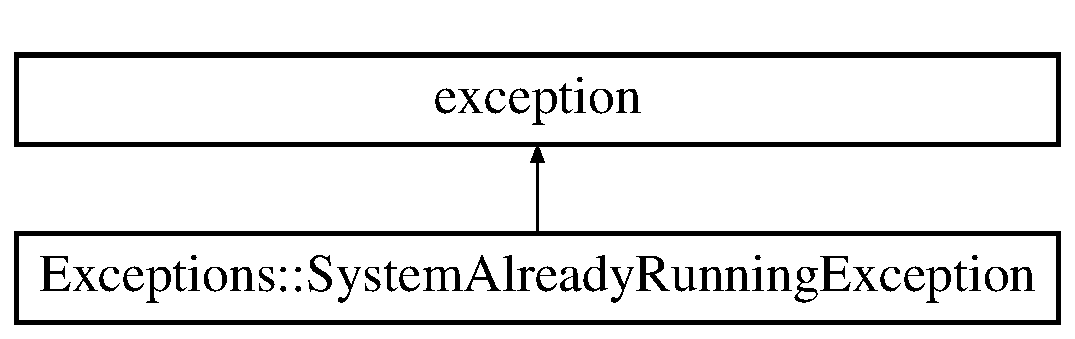
\includegraphics[height=2.000000cm]{class_exceptions_1_1_system_already_running_exception}
\end{center}
\end{figure}
\subsection*{Public Member Functions}
\begin{DoxyCompactItemize}
\item 
\hyperlink{class_exceptions_1_1_system_already_running_exception_aed8f9f444543924acea118e7485fdbba}{System\+Already\+Running\+Exception} (std\+::string \hyperlink{class_exceptions_1_1_system_already_running_exception_a914a5cb77c9acbd05862c8927da7ea36}{system\+\_\+name})
\item 
virtual const char $\ast$ \hyperlink{class_exceptions_1_1_system_already_running_exception_a558ddbeefc7c578b0a2c7ac031a5aef5}{what} () const   throw ()
\end{DoxyCompactItemize}
\subsection*{Private Attributes}
\begin{DoxyCompactItemize}
\item 
std\+::string \hyperlink{class_exceptions_1_1_system_already_running_exception_a914a5cb77c9acbd05862c8927da7ea36}{system\+\_\+name}
\end{DoxyCompactItemize}


\subsection{Constructor \& Destructor Documentation}
\hypertarget{class_exceptions_1_1_system_already_running_exception_aed8f9f444543924acea118e7485fdbba}{}\index{Exceptions\+::\+System\+Already\+Running\+Exception@{Exceptions\+::\+System\+Already\+Running\+Exception}!System\+Already\+Running\+Exception@{System\+Already\+Running\+Exception}}
\index{System\+Already\+Running\+Exception@{System\+Already\+Running\+Exception}!Exceptions\+::\+System\+Already\+Running\+Exception@{Exceptions\+::\+System\+Already\+Running\+Exception}}
\subsubsection[{System\+Already\+Running\+Exception}]{\setlength{\rightskip}{0pt plus 5cm}Exceptions\+::\+System\+Already\+Running\+Exception\+::\+System\+Already\+Running\+Exception (
\begin{DoxyParamCaption}
\item[{std\+::string}]{system\+\_\+name}
\end{DoxyParamCaption}
)\hspace{0.3cm}{\ttfamily [inline]}}\label{class_exceptions_1_1_system_already_running_exception_aed8f9f444543924acea118e7485fdbba}


\subsection{Member Function Documentation}
\hypertarget{class_exceptions_1_1_system_already_running_exception_a558ddbeefc7c578b0a2c7ac031a5aef5}{}\index{Exceptions\+::\+System\+Already\+Running\+Exception@{Exceptions\+::\+System\+Already\+Running\+Exception}!what@{what}}
\index{what@{what}!Exceptions\+::\+System\+Already\+Running\+Exception@{Exceptions\+::\+System\+Already\+Running\+Exception}}
\subsubsection[{what}]{\setlength{\rightskip}{0pt plus 5cm}virtual const char$\ast$ Exceptions\+::\+System\+Already\+Running\+Exception\+::what (
\begin{DoxyParamCaption}
{}
\end{DoxyParamCaption}
) const throw  ) \hspace{0.3cm}{\ttfamily [inline]}, {\ttfamily [virtual]}}\label{class_exceptions_1_1_system_already_running_exception_a558ddbeefc7c578b0a2c7ac031a5aef5}


\subsection{Member Data Documentation}
\hypertarget{class_exceptions_1_1_system_already_running_exception_a914a5cb77c9acbd05862c8927da7ea36}{}\index{Exceptions\+::\+System\+Already\+Running\+Exception@{Exceptions\+::\+System\+Already\+Running\+Exception}!system\+\_\+name@{system\+\_\+name}}
\index{system\+\_\+name@{system\+\_\+name}!Exceptions\+::\+System\+Already\+Running\+Exception@{Exceptions\+::\+System\+Already\+Running\+Exception}}
\subsubsection[{system\+\_\+name}]{\setlength{\rightskip}{0pt plus 5cm}std\+::string Exceptions\+::\+System\+Already\+Running\+Exception\+::system\+\_\+name\hspace{0.3cm}{\ttfamily [private]}}\label{class_exceptions_1_1_system_already_running_exception_a914a5cb77c9acbd05862c8927da7ea36}


The documentation for this class was generated from the following file\+:\begin{DoxyCompactItemize}
\item 
src/exceptions/\hyperlink{system__already__running__exception_8h}{system\+\_\+already\+\_\+running\+\_\+exception.\+h}\end{DoxyCompactItemize}

\hypertarget{class_exceptions_1_1_system_not_initialized_exception}{}\section{Exceptions\+:\+:System\+Not\+Initialized\+Exception Class Reference}
\label{class_exceptions_1_1_system_not_initialized_exception}\index{Exceptions\+::\+System\+Not\+Initialized\+Exception@{Exceptions\+::\+System\+Not\+Initialized\+Exception}}


{\ttfamily \#include $<$system\+\_\+not\+\_\+initialized\+\_\+exception.\+h$>$}

Inheritance diagram for Exceptions\+:\+:System\+Not\+Initialized\+Exception\+:\begin{figure}[H]
\begin{center}
\leavevmode
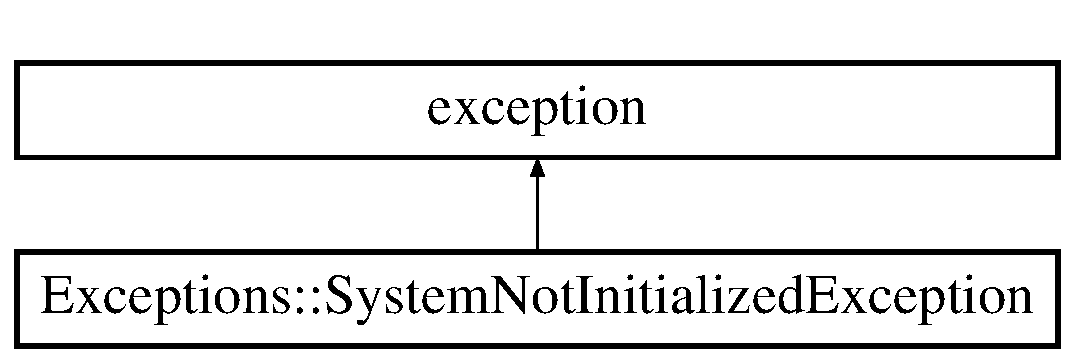
\includegraphics[height=2.000000cm]{class_exceptions_1_1_system_not_initialized_exception}
\end{center}
\end{figure}
\subsection*{Public Member Functions}
\begin{DoxyCompactItemize}
\item 
\hyperlink{class_exceptions_1_1_system_not_initialized_exception_ac22625946ad8f784f8c78b1b5b2970d7}{System\+Not\+Initialized\+Exception} (std\+::string \hyperlink{class_exceptions_1_1_system_not_initialized_exception_a5649bbb869394d52f7c8aa82d600d070}{system\+\_\+name})
\item 
virtual const char $\ast$ \hyperlink{class_exceptions_1_1_system_not_initialized_exception_a6481e3f2f2dd245e47ed246b12ce61c5}{what} () const   throw ()
\end{DoxyCompactItemize}
\subsection*{Private Attributes}
\begin{DoxyCompactItemize}
\item 
std\+::string \hyperlink{class_exceptions_1_1_system_not_initialized_exception_a5649bbb869394d52f7c8aa82d600d070}{system\+\_\+name}
\end{DoxyCompactItemize}


\subsection{Constructor \& Destructor Documentation}
\hypertarget{class_exceptions_1_1_system_not_initialized_exception_ac22625946ad8f784f8c78b1b5b2970d7}{}\index{Exceptions\+::\+System\+Not\+Initialized\+Exception@{Exceptions\+::\+System\+Not\+Initialized\+Exception}!System\+Not\+Initialized\+Exception@{System\+Not\+Initialized\+Exception}}
\index{System\+Not\+Initialized\+Exception@{System\+Not\+Initialized\+Exception}!Exceptions\+::\+System\+Not\+Initialized\+Exception@{Exceptions\+::\+System\+Not\+Initialized\+Exception}}
\subsubsection[{System\+Not\+Initialized\+Exception}]{\setlength{\rightskip}{0pt plus 5cm}Exceptions\+::\+System\+Not\+Initialized\+Exception\+::\+System\+Not\+Initialized\+Exception (
\begin{DoxyParamCaption}
\item[{std\+::string}]{system\+\_\+name}
\end{DoxyParamCaption}
)\hspace{0.3cm}{\ttfamily [inline]}}\label{class_exceptions_1_1_system_not_initialized_exception_ac22625946ad8f784f8c78b1b5b2970d7}


\subsection{Member Function Documentation}
\hypertarget{class_exceptions_1_1_system_not_initialized_exception_a6481e3f2f2dd245e47ed246b12ce61c5}{}\index{Exceptions\+::\+System\+Not\+Initialized\+Exception@{Exceptions\+::\+System\+Not\+Initialized\+Exception}!what@{what}}
\index{what@{what}!Exceptions\+::\+System\+Not\+Initialized\+Exception@{Exceptions\+::\+System\+Not\+Initialized\+Exception}}
\subsubsection[{what}]{\setlength{\rightskip}{0pt plus 5cm}virtual const char$\ast$ Exceptions\+::\+System\+Not\+Initialized\+Exception\+::what (
\begin{DoxyParamCaption}
{}
\end{DoxyParamCaption}
) const throw  ) \hspace{0.3cm}{\ttfamily [inline]}, {\ttfamily [virtual]}}\label{class_exceptions_1_1_system_not_initialized_exception_a6481e3f2f2dd245e47ed246b12ce61c5}


\subsection{Member Data Documentation}
\hypertarget{class_exceptions_1_1_system_not_initialized_exception_a5649bbb869394d52f7c8aa82d600d070}{}\index{Exceptions\+::\+System\+Not\+Initialized\+Exception@{Exceptions\+::\+System\+Not\+Initialized\+Exception}!system\+\_\+name@{system\+\_\+name}}
\index{system\+\_\+name@{system\+\_\+name}!Exceptions\+::\+System\+Not\+Initialized\+Exception@{Exceptions\+::\+System\+Not\+Initialized\+Exception}}
\subsubsection[{system\+\_\+name}]{\setlength{\rightskip}{0pt plus 5cm}std\+::string Exceptions\+::\+System\+Not\+Initialized\+Exception\+::system\+\_\+name\hspace{0.3cm}{\ttfamily [private]}}\label{class_exceptions_1_1_system_not_initialized_exception_a5649bbb869394d52f7c8aa82d600d070}


The documentation for this class was generated from the following file\+:\begin{DoxyCompactItemize}
\item 
src/exceptions/\hyperlink{system__not__initialized__exception_8h}{system\+\_\+not\+\_\+initialized\+\_\+exception.\+h}\end{DoxyCompactItemize}

\hypertarget{class_exceptions_1_1_system_not_running_exception}{}\section{Exceptions\+:\+:System\+Not\+Running\+Exception Class Reference}
\label{class_exceptions_1_1_system_not_running_exception}\index{Exceptions\+::\+System\+Not\+Running\+Exception@{Exceptions\+::\+System\+Not\+Running\+Exception}}


{\ttfamily \#include $<$system\+\_\+not\+\_\+running\+\_\+exception.\+h$>$}

Inheritance diagram for Exceptions\+:\+:System\+Not\+Running\+Exception\+:\begin{figure}[H]
\begin{center}
\leavevmode
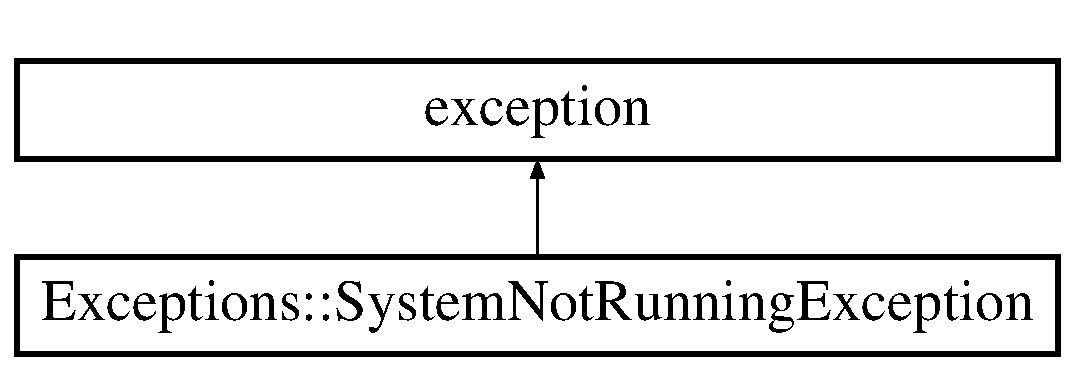
\includegraphics[height=2.000000cm]{class_exceptions_1_1_system_not_running_exception}
\end{center}
\end{figure}
\subsection*{Public Member Functions}
\begin{DoxyCompactItemize}
\item 
\hyperlink{class_exceptions_1_1_system_not_running_exception_aed32e775ba2eb68ff70446c138c40bcc}{System\+Not\+Running\+Exception} (std\+::string \hyperlink{class_exceptions_1_1_system_not_running_exception_af97cd0ba9e5c5b4aa57b99028b6bb95a}{system\+\_\+name})
\item 
virtual const char $\ast$ \hyperlink{class_exceptions_1_1_system_not_running_exception_afc7a24ce91303377321104405996f5ff}{what} () const   throw ()
\end{DoxyCompactItemize}
\subsection*{Private Attributes}
\begin{DoxyCompactItemize}
\item 
std\+::string \hyperlink{class_exceptions_1_1_system_not_running_exception_af97cd0ba9e5c5b4aa57b99028b6bb95a}{system\+\_\+name}
\end{DoxyCompactItemize}


\subsection{Constructor \& Destructor Documentation}
\hypertarget{class_exceptions_1_1_system_not_running_exception_aed32e775ba2eb68ff70446c138c40bcc}{}\index{Exceptions\+::\+System\+Not\+Running\+Exception@{Exceptions\+::\+System\+Not\+Running\+Exception}!System\+Not\+Running\+Exception@{System\+Not\+Running\+Exception}}
\index{System\+Not\+Running\+Exception@{System\+Not\+Running\+Exception}!Exceptions\+::\+System\+Not\+Running\+Exception@{Exceptions\+::\+System\+Not\+Running\+Exception}}
\subsubsection[{System\+Not\+Running\+Exception}]{\setlength{\rightskip}{0pt plus 5cm}Exceptions\+::\+System\+Not\+Running\+Exception\+::\+System\+Not\+Running\+Exception (
\begin{DoxyParamCaption}
\item[{std\+::string}]{system\+\_\+name}
\end{DoxyParamCaption}
)\hspace{0.3cm}{\ttfamily [inline]}}\label{class_exceptions_1_1_system_not_running_exception_aed32e775ba2eb68ff70446c138c40bcc}


\subsection{Member Function Documentation}
\hypertarget{class_exceptions_1_1_system_not_running_exception_afc7a24ce91303377321104405996f5ff}{}\index{Exceptions\+::\+System\+Not\+Running\+Exception@{Exceptions\+::\+System\+Not\+Running\+Exception}!what@{what}}
\index{what@{what}!Exceptions\+::\+System\+Not\+Running\+Exception@{Exceptions\+::\+System\+Not\+Running\+Exception}}
\subsubsection[{what}]{\setlength{\rightskip}{0pt plus 5cm}virtual const char$\ast$ Exceptions\+::\+System\+Not\+Running\+Exception\+::what (
\begin{DoxyParamCaption}
{}
\end{DoxyParamCaption}
) const throw  ) \hspace{0.3cm}{\ttfamily [inline]}, {\ttfamily [virtual]}}\label{class_exceptions_1_1_system_not_running_exception_afc7a24ce91303377321104405996f5ff}


\subsection{Member Data Documentation}
\hypertarget{class_exceptions_1_1_system_not_running_exception_af97cd0ba9e5c5b4aa57b99028b6bb95a}{}\index{Exceptions\+::\+System\+Not\+Running\+Exception@{Exceptions\+::\+System\+Not\+Running\+Exception}!system\+\_\+name@{system\+\_\+name}}
\index{system\+\_\+name@{system\+\_\+name}!Exceptions\+::\+System\+Not\+Running\+Exception@{Exceptions\+::\+System\+Not\+Running\+Exception}}
\subsubsection[{system\+\_\+name}]{\setlength{\rightskip}{0pt plus 5cm}std\+::string Exceptions\+::\+System\+Not\+Running\+Exception\+::system\+\_\+name\hspace{0.3cm}{\ttfamily [private]}}\label{class_exceptions_1_1_system_not_running_exception_af97cd0ba9e5c5b4aa57b99028b6bb95a}


The documentation for this class was generated from the following file\+:\begin{DoxyCompactItemize}
\item 
src/exceptions/\hyperlink{system__not__running__exception_8h}{system\+\_\+not\+\_\+running\+\_\+exception.\+h}\end{DoxyCompactItemize}

\hypertarget{class_test_attribute_trait}{}\section{Test\+Attribute\+Trait Class Reference}
\label{class_test_attribute_trait}\index{Test\+Attribute\+Trait@{Test\+Attribute\+Trait}}
Inheritance diagram for Test\+Attribute\+Trait\+:\begin{figure}[H]
\begin{center}
\leavevmode
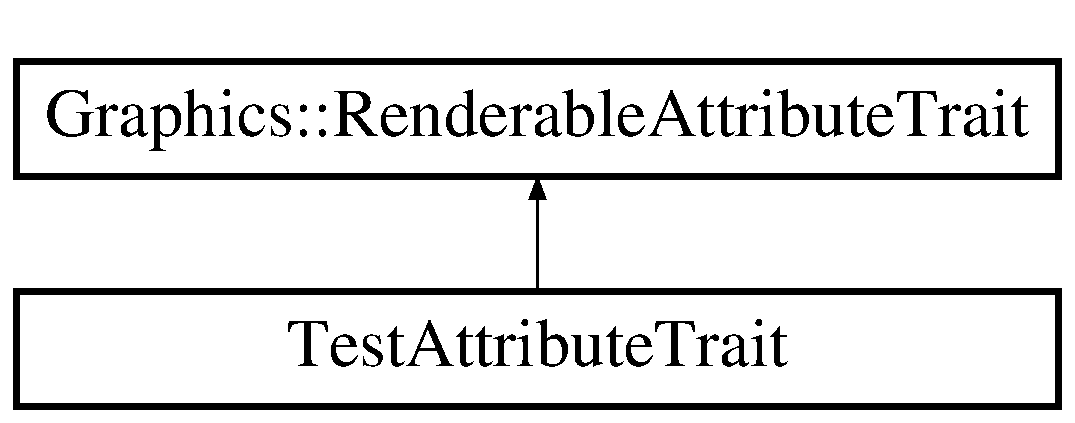
\includegraphics[height=3.000000cm]{class_test_attribute_trait}
\end{center}
\end{figure}
\subsection*{Public Member Functions}
\begin{DoxyCompactItemize}
\item 
\hyperlink{class_test_attribute_trait_abf91ded2bc981ff07f82f5808291aa27}{Test\+Attribute\+Trait} ()
\item 
virtual const std\+::map$<$ \hyperlink{class_graphics_1_1_vertex_data_a50e88236939dc2a3ec4df7aeb728620e}{Graphics\+::\+Vertex\+Data\+::\+D\+A\+T\+A\+\_\+\+T\+Y\+P\+E}, unsigned int $>$ \hyperlink{class_test_attribute_trait_af121ef5fbd5bcda4bbbc7fdadd5599c8}{operator()} () const noexceptoverride
\end{DoxyCompactItemize}
\subsection*{Private Attributes}
\begin{DoxyCompactItemize}
\item 
std\+::map$<$ \hyperlink{class_graphics_1_1_vertex_data_a50e88236939dc2a3ec4df7aeb728620e}{Graphics\+::\+Vertex\+Data\+::\+D\+A\+T\+A\+\_\+\+T\+Y\+P\+E}, unsigned int $>$ \hyperlink{class_test_attribute_trait_a4e8fa71f7e6ced6e221c08a5a19a46a5}{trait}
\end{DoxyCompactItemize}


\subsection{Constructor \& Destructor Documentation}
\hypertarget{class_test_attribute_trait_abf91ded2bc981ff07f82f5808291aa27}{}\index{Test\+Attribute\+Trait@{Test\+Attribute\+Trait}!Test\+Attribute\+Trait@{Test\+Attribute\+Trait}}
\index{Test\+Attribute\+Trait@{Test\+Attribute\+Trait}!Test\+Attribute\+Trait@{Test\+Attribute\+Trait}}
\subsubsection[{Test\+Attribute\+Trait}]{\setlength{\rightskip}{0pt plus 5cm}Test\+Attribute\+Trait\+::\+Test\+Attribute\+Trait (
\begin{DoxyParamCaption}
{}
\end{DoxyParamCaption}
)\hspace{0.3cm}{\ttfamily [inline]}}\label{class_test_attribute_trait_abf91ded2bc981ff07f82f5808291aa27}


\subsection{Member Function Documentation}
\hypertarget{class_test_attribute_trait_af121ef5fbd5bcda4bbbc7fdadd5599c8}{}\index{Test\+Attribute\+Trait@{Test\+Attribute\+Trait}!operator()@{operator()}}
\index{operator()@{operator()}!Test\+Attribute\+Trait@{Test\+Attribute\+Trait}}
\subsubsection[{operator()}]{\setlength{\rightskip}{0pt plus 5cm}virtual const std\+::map$<${\bf Graphics\+::\+Vertex\+Data\+::\+D\+A\+T\+A\+\_\+\+T\+Y\+P\+E}, unsigned int$>$ Test\+Attribute\+Trait\+::operator() (
\begin{DoxyParamCaption}
{}
\end{DoxyParamCaption}
) const\hspace{0.3cm}{\ttfamily [inline]}, {\ttfamily [override]}, {\ttfamily [virtual]}, {\ttfamily [noexcept]}}\label{class_test_attribute_trait_af121ef5fbd5bcda4bbbc7fdadd5599c8}


Reimplemented from \hyperlink{class_graphics_1_1_renderable_attribute_trait_a44401f624ace1dc71220e7064db92465}{Graphics\+::\+Renderable\+Attribute\+Trait}.



\subsection{Member Data Documentation}
\hypertarget{class_test_attribute_trait_a4e8fa71f7e6ced6e221c08a5a19a46a5}{}\index{Test\+Attribute\+Trait@{Test\+Attribute\+Trait}!trait@{trait}}
\index{trait@{trait}!Test\+Attribute\+Trait@{Test\+Attribute\+Trait}}
\subsubsection[{trait}]{\setlength{\rightskip}{0pt plus 5cm}std\+::map$<${\bf Graphics\+::\+Vertex\+Data\+::\+D\+A\+T\+A\+\_\+\+T\+Y\+P\+E}, unsigned int$>$ Test\+Attribute\+Trait\+::trait\hspace{0.3cm}{\ttfamily [private]}}\label{class_test_attribute_trait_a4e8fa71f7e6ced6e221c08a5a19a46a5}


The documentation for this class was generated from the following file\+:\begin{DoxyCompactItemize}
\item 
test/graphics/\hyperlink{renderable__test_8cpp}{renderable\+\_\+test.\+cpp}\end{DoxyCompactItemize}

\hypertarget{class_graphics_1_1_tile_attribute_trait}{}\section{Graphics\+:\+:Tile\+Attribute\+Trait Class Reference}
\label{class_graphics_1_1_tile_attribute_trait}\index{Graphics\+::\+Tile\+Attribute\+Trait@{Graphics\+::\+Tile\+Attribute\+Trait}}


{\ttfamily \#include $<$tile\+\_\+attribute\+\_\+trait.\+h$>$}

Inheritance diagram for Graphics\+:\+:Tile\+Attribute\+Trait\+:\begin{figure}[H]
\begin{center}
\leavevmode
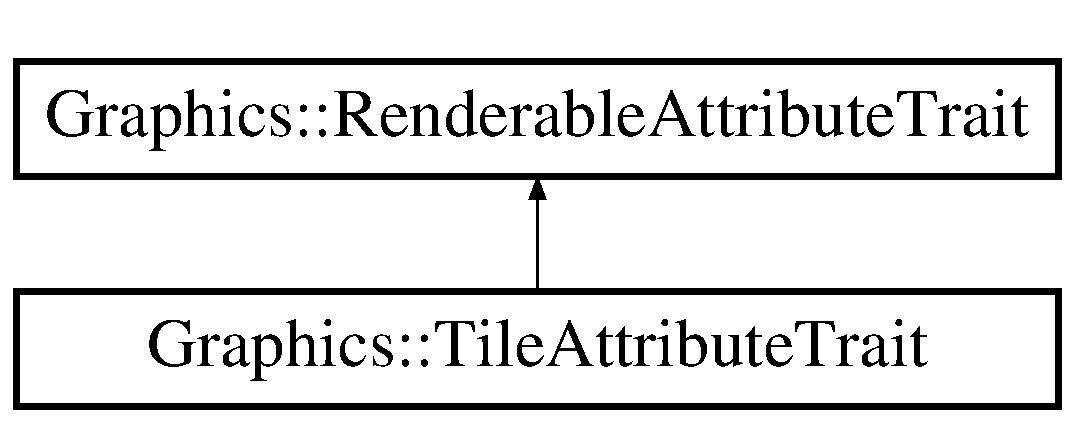
\includegraphics[height=2.000000cm]{class_graphics_1_1_tile_attribute_trait}
\end{center}
\end{figure}
\subsection*{Public Member Functions}
\begin{DoxyCompactItemize}
\item 
\hyperlink{class_graphics_1_1_tile_attribute_trait_a8271798aeb430ac5cf3dc1a0c73175fd}{Tile\+Attribute\+Trait} ()
\item 
virtual const std\+::map$<$ \hyperlink{class_graphics_1_1_vertex_data_a50e88236939dc2a3ec4df7aeb728620e}{Vertex\+Data\+::\+D\+A\+T\+A\+\_\+\+T\+Y\+P\+E}, unsigned int $>$ \hyperlink{class_graphics_1_1_tile_attribute_trait_a5c217a080f9b52799ad6c9e2ffaa06f5}{operator()} () const noexceptoverride
\end{DoxyCompactItemize}
\subsection*{Private Attributes}
\begin{DoxyCompactItemize}
\item 
std\+::map$<$ \hyperlink{class_graphics_1_1_vertex_data_a50e88236939dc2a3ec4df7aeb728620e}{Vertex\+Data\+::\+D\+A\+T\+A\+\_\+\+T\+Y\+P\+E}, unsigned int $>$ \hyperlink{class_graphics_1_1_tile_attribute_trait_a207820d288507ca70df8f95d7fdd04db}{trait}
\end{DoxyCompactItemize}


\subsection{Constructor \& Destructor Documentation}
\hypertarget{class_graphics_1_1_tile_attribute_trait_a8271798aeb430ac5cf3dc1a0c73175fd}{}\index{Graphics\+::\+Tile\+Attribute\+Trait@{Graphics\+::\+Tile\+Attribute\+Trait}!Tile\+Attribute\+Trait@{Tile\+Attribute\+Trait}}
\index{Tile\+Attribute\+Trait@{Tile\+Attribute\+Trait}!Graphics\+::\+Tile\+Attribute\+Trait@{Graphics\+::\+Tile\+Attribute\+Trait}}
\subsubsection[{Tile\+Attribute\+Trait}]{\setlength{\rightskip}{0pt plus 5cm}Graphics\+::\+Tile\+Attribute\+Trait\+::\+Tile\+Attribute\+Trait (
\begin{DoxyParamCaption}
{}
\end{DoxyParamCaption}
)\hspace{0.3cm}{\ttfamily [inline]}}\label{class_graphics_1_1_tile_attribute_trait_a8271798aeb430ac5cf3dc1a0c73175fd}


\subsection{Member Function Documentation}
\hypertarget{class_graphics_1_1_tile_attribute_trait_a5c217a080f9b52799ad6c9e2ffaa06f5}{}\index{Graphics\+::\+Tile\+Attribute\+Trait@{Graphics\+::\+Tile\+Attribute\+Trait}!operator()@{operator()}}
\index{operator()@{operator()}!Graphics\+::\+Tile\+Attribute\+Trait@{Graphics\+::\+Tile\+Attribute\+Trait}}
\subsubsection[{operator()}]{\setlength{\rightskip}{0pt plus 5cm}virtual const std\+::map$<${\bf Vertex\+Data\+::\+D\+A\+T\+A\+\_\+\+T\+Y\+P\+E}, unsigned int$>$ Graphics\+::\+Tile\+Attribute\+Trait\+::operator() (
\begin{DoxyParamCaption}
{}
\end{DoxyParamCaption}
) const\hspace{0.3cm}{\ttfamily [inline]}, {\ttfamily [override]}, {\ttfamily [virtual]}, {\ttfamily [noexcept]}}\label{class_graphics_1_1_tile_attribute_trait_a5c217a080f9b52799ad6c9e2ffaa06f5}


Implements \hyperlink{class_graphics_1_1_base_attribute_trait_a7f43cabd619b64be1a0056e0fe568cf5}{Graphics\+::\+Base\+Attribute\+Trait}.



\subsection{Member Data Documentation}
\hypertarget{class_graphics_1_1_tile_attribute_trait_a207820d288507ca70df8f95d7fdd04db}{}\index{Graphics\+::\+Tile\+Attribute\+Trait@{Graphics\+::\+Tile\+Attribute\+Trait}!trait@{trait}}
\index{trait@{trait}!Graphics\+::\+Tile\+Attribute\+Trait@{Graphics\+::\+Tile\+Attribute\+Trait}}
\subsubsection[{trait}]{\setlength{\rightskip}{0pt plus 5cm}std\+::map$<${\bf Vertex\+Data\+::\+D\+A\+T\+A\+\_\+\+T\+Y\+P\+E}, unsigned int$>$ Graphics\+::\+Tile\+Attribute\+Trait\+::trait\hspace{0.3cm}{\ttfamily [private]}}\label{class_graphics_1_1_tile_attribute_trait_a207820d288507ca70df8f95d7fdd04db}


The documentation for this class was generated from the following file\+:\begin{DoxyCompactItemize}
\item 
src/graphics/\hyperlink{tile__attribute__trait_8h}{tile\+\_\+attribute\+\_\+trait.\+h}\end{DoxyCompactItemize}

\hypertarget{class_graphics_1_1_vertex_data}{}\section{Graphics\+:\+:Vertex\+Data Class Reference}
\label{class_graphics_1_1_vertex_data}\index{Graphics\+::\+Vertex\+Data@{Graphics\+::\+Vertex\+Data}}


{\ttfamily \#include $<$vertex\+\_\+data.\+h$>$}

\subsection*{Public Types}
\begin{DoxyCompactItemize}
\item 
enum \hyperlink{class_graphics_1_1_vertex_data_a50e88236939dc2a3ec4df7aeb728620e}{D\+A\+T\+A\+\_\+\+T\+Y\+P\+E} \+: unsigned char \{ \\*
\hyperlink{class_graphics_1_1_vertex_data_a50e88236939dc2a3ec4df7aeb728620eab4b2880ea86c8ee2eaceee4fbf35d3ac}{G\+E\+O\+M\+E\+T\+R\+Y} = 0, 
\hyperlink{class_graphics_1_1_vertex_data_a50e88236939dc2a3ec4df7aeb728620ea7b93224f58c43662f5be328f032d01e4}{T\+E\+X\+\_\+\+C\+O\+O\+R\+D\+S} = 1, 
\hyperlink{class_graphics_1_1_vertex_data_a50e88236939dc2a3ec4df7aeb728620ea0dbe0aa86a7dc55ca3aef237b0084068}{N\+O\+R\+M\+A\+L\+\_\+\+C\+O\+O\+R\+D\+S} = 2, 
\hyperlink{class_graphics_1_1_vertex_data_a50e88236939dc2a3ec4df7aeb728620ea77588319217115a8d9dead081e341e83}{R\+E\+S\+E\+R\+V\+E\+D1} = 3, 
\\*
\hyperlink{class_graphics_1_1_vertex_data_a50e88236939dc2a3ec4df7aeb728620ea9c6b6dd55ddf236f667e3e4019cda8d7}{R\+E\+S\+E\+R\+V\+E\+D2} = 4, 
\hyperlink{class_graphics_1_1_vertex_data_a50e88236939dc2a3ec4df7aeb728620eafc91ad501328ae49126c5d4bf850e537}{R\+E\+S\+E\+R\+V\+E\+D3} = 5, 
\hyperlink{class_graphics_1_1_vertex_data_a50e88236939dc2a3ec4df7aeb728620ea2185ed1920c6eeea484c4050e149764d}{R\+E\+S\+E\+R\+V\+E\+D4} = 6, 
\hyperlink{class_graphics_1_1_vertex_data_a50e88236939dc2a3ec4df7aeb728620ea92ff06fddd97b8c7d306ff7e912aeaba}{R\+E\+S\+E\+R\+V\+E\+D5} = 7, 
\\*
\hyperlink{class_graphics_1_1_vertex_data_a50e88236939dc2a3ec4df7aeb728620ea815ed3d3f65efe3a61a3df584a8fad55}{R\+E\+S\+E\+R\+V\+E\+D6} = 8, 
\hyperlink{class_graphics_1_1_vertex_data_a50e88236939dc2a3ec4df7aeb728620ead297e598e1a3dd7e9f7f3cc624130de9}{R\+E\+S\+E\+R\+V\+E\+D7} = 9, 
\hyperlink{class_graphics_1_1_vertex_data_a50e88236939dc2a3ec4df7aeb728620ea8f0a8e69a480d1dfb0f671acd6f72249}{R\+E\+S\+E\+R\+V\+E\+D8} = 10, 
\hyperlink{class_graphics_1_1_vertex_data_a50e88236939dc2a3ec4df7aeb728620eaeef1b1af84ab650ca26fcd90ed548642}{R\+E\+S\+E\+R\+V\+E\+D9} = 11, 
\\*
\hyperlink{class_graphics_1_1_vertex_data_a50e88236939dc2a3ec4df7aeb728620eaca1c371d86cb760f697bc8f9269ccc3a}{O\+N\+E\+\_\+\+W\+I\+D\+E} = 12, 
\hyperlink{class_graphics_1_1_vertex_data_a50e88236939dc2a3ec4df7aeb728620eaf411c36479247811d74f8c389cf22a9e}{T\+W\+O\+\_\+\+W\+I\+D\+E} = 13, 
\hyperlink{class_graphics_1_1_vertex_data_a50e88236939dc2a3ec4df7aeb728620eaed7cce23f542ae67236d1f0612bedce3}{T\+H\+R\+E\+E\+\_\+\+W\+I\+D\+E} = 14, 
\hyperlink{class_graphics_1_1_vertex_data_a50e88236939dc2a3ec4df7aeb728620eabcba96d8df23979f402ee0d3fbc22357}{F\+O\+U\+R\+\_\+\+W\+I\+D\+E} = 15
 \}
\end{DoxyCompactItemize}
\subsection*{Public Member Functions}
\begin{DoxyCompactItemize}
\item 
\hyperlink{class_graphics_1_1_vertex_data_a5f7a4162413a61c94cba76b528c17cc6}{Vertex\+Data} ()=delete
\item 
\hyperlink{class_graphics_1_1_vertex_data_aab133d7bc7567df43e6055f81e2ed23c}{Vertex\+Data} (const G\+Lenum \hyperlink{class_graphics_1_1_vertex_data_a3940832a3699c42ea2d9f4e0943653aa}{primitive\+\_\+type})
\item 
\hyperlink{class_graphics_1_1_vertex_data_aaf7331434454cb253f5ad5b86a8eec99}{Vertex\+Data} (const \hyperlink{class_graphics_1_1_vertex_data}{Vertex\+Data} \&vertex\+\_\+data)
\item 
\hyperlink{class_graphics_1_1_vertex_data}{Vertex\+Data} \hyperlink{class_graphics_1_1_vertex_data_abda73a49d1b280ee091afd53973c3448}{operator=} (const \hyperlink{class_graphics_1_1_vertex_data}{Vertex\+Data} \&vertex\+\_\+data)
\item 
\hyperlink{class_graphics_1_1_vertex_data_a59b5214fe3d6b6f9425032c86abf65cb}{$\sim$\+Vertex\+Data} ()
\item 
const bool \hyperlink{class_graphics_1_1_vertex_data_ad58ef98925908992fcd3ff090f57693f}{operator==} (const \hyperlink{class_graphics_1_1_vertex_data}{Vertex\+Data} \&other)
\item 
const bool \hyperlink{class_graphics_1_1_vertex_data_ac03511a02af7005757f60783b73fc51f}{operator!=} (const \hyperlink{class_graphics_1_1_vertex_data}{Vertex\+Data} \&other)
\item 
void \hyperlink{class_graphics_1_1_vertex_data_a9d7dfbf44faa4ebeeb052d9a49ec72c4}{add\+Indices} (const std\+::vector$<$ unsigned int $>$ \&\hyperlink{class_graphics_1_1_vertex_data_a9b777aa4bf035e805b2957fbcd158842}{indices})
\item 
{\footnotesize template$<$typename T $>$ }\\void \hyperlink{class_graphics_1_1_vertex_data_a1432af05a48b67a06c711910bb495c6e}{add\+Vec} (\hyperlink{class_graphics_1_1_vertex_data_a50e88236939dc2a3ec4df7aeb728620e}{D\+A\+T\+A\+\_\+\+T\+Y\+P\+E} data\+\_\+type, const std\+::vector$<$ T $>$ \&vec)
\item 
const unsigned int \hyperlink{class_graphics_1_1_vertex_data_a0c58a46431db14740109e6cadb322e4e}{get\+Index\+Count} () const noexcept
\item 
const unsigned int \hyperlink{class_graphics_1_1_vertex_data_afc9fb219a54d93cc0796424bd9d1a7db}{get\+Vertex\+Count} () const noexcept
\item 
{\footnotesize template$<$typename T $>$ }\\std\+::map$<$ \hyperlink{class_graphics_1_1_vertex_data_a50e88236939dc2a3ec4df7aeb728620e}{D\+A\+T\+A\+\_\+\+T\+Y\+P\+E}, std\+::vector$<$ T $>$ $>$ \hyperlink{class_graphics_1_1_vertex_data_a860575a29aa889f2a1028f2b8a255adc}{get\+Collapsed\+Vectors} () const 
\item 
std\+::vector$<$ unsigned int $>$ \hyperlink{class_graphics_1_1_vertex_data_a39b62d7b756b924aed1025d725a2316a}{get\+Indices} () const noexcept
\item 
unsigned int \hyperlink{class_graphics_1_1_vertex_data_ae46d393d65961b336a380d22bc8e39cb}{number\+Vertex\+Buffer\+Objects} () const noexcept
\item 
{\footnotesize template$<$$>$ }\\void \hyperlink{class_graphics_1_1_vertex_data_a3c16815abdf03faa1789af508f378b4a}{add\+Vec} (\hyperlink{class_graphics_1_1_vertex_data_a50e88236939dc2a3ec4df7aeb728620e}{Vertex\+Data\+::\+D\+A\+T\+A\+\_\+\+T\+Y\+P\+E} data\+\_\+type, const std\+::vector$<$ float $>$ \&vec)
\item 
{\footnotesize template$<$$>$ }\\void \hyperlink{class_graphics_1_1_vertex_data_a718710cb36c77da3ce7202fbf78f9dcf}{add\+Vec} (\hyperlink{class_graphics_1_1_vertex_data_a50e88236939dc2a3ec4df7aeb728620e}{Vertex\+Data\+::\+D\+A\+T\+A\+\_\+\+T\+Y\+P\+E} data\+\_\+type, const std\+::vector$<$ double $>$ \&vec)
\item 
{\footnotesize template$<$$>$ }\\void \hyperlink{class_graphics_1_1_vertex_data_addc04a692143dbd59ef3eb1b9107afc9}{add\+Vec} (\hyperlink{class_graphics_1_1_vertex_data_a50e88236939dc2a3ec4df7aeb728620e}{Vertex\+Data\+::\+D\+A\+T\+A\+\_\+\+T\+Y\+P\+E} data\+\_\+type, const std\+::vector$<$ int $>$ \&vec)
\item 
{\footnotesize template$<$$>$ }\\void \hyperlink{class_graphics_1_1_vertex_data_ad5b58302a2e592db88a896f8e8cbd83d}{add\+Vec} (\hyperlink{class_graphics_1_1_vertex_data_a50e88236939dc2a3ec4df7aeb728620e}{Vertex\+Data\+::\+D\+A\+T\+A\+\_\+\+T\+Y\+P\+E} data\+\_\+type, const std\+::vector$<$ unsigned int $>$ \&vec)
\item 
{\footnotesize template$<$$>$ }\\std\+::map$<$ \hyperlink{class_graphics_1_1_vertex_data_a50e88236939dc2a3ec4df7aeb728620e}{Vertex\+Data\+::\+D\+A\+T\+A\+\_\+\+T\+Y\+P\+E}, std\+::vector$<$ float $>$ $>$ \hyperlink{class_graphics_1_1_vertex_data_a248ab37b8eec5e4befba68c09a56fc1b}{get\+Collapsed\+Vectors} () const 
\item 
{\footnotesize template$<$$>$ }\\std\+::map$<$ \hyperlink{class_graphics_1_1_vertex_data_a50e88236939dc2a3ec4df7aeb728620e}{Vertex\+Data\+::\+D\+A\+T\+A\+\_\+\+T\+Y\+P\+E}, std\+::vector$<$ double $>$ $>$ \hyperlink{class_graphics_1_1_vertex_data_a460ef7490af53909849ede22d63f3144}{get\+Collapsed\+Vectors} () const 
\item 
{\footnotesize template$<$$>$ }\\std\+::map$<$ \hyperlink{class_graphics_1_1_vertex_data_a50e88236939dc2a3ec4df7aeb728620e}{Vertex\+Data\+::\+D\+A\+T\+A\+\_\+\+T\+Y\+P\+E}, std\+::vector$<$ int $>$ $>$ \hyperlink{class_graphics_1_1_vertex_data_a198830ed9c9eaadd45776b17bfa2909d}{get\+Collapsed\+Vectors} () const 
\item 
{\footnotesize template$<$$>$ }\\std\+::map$<$ \hyperlink{class_graphics_1_1_vertex_data_a50e88236939dc2a3ec4df7aeb728620e}{Vertex\+Data\+::\+D\+A\+T\+A\+\_\+\+T\+Y\+P\+E}, std\+::vector$<$ unsigned int $>$ $>$ \hyperlink{class_graphics_1_1_vertex_data_a1a056a887e89425563b93c7d14402a21}{get\+Collapsed\+Vectors} () const 
\end{DoxyCompactItemize}
\subsection*{Static Public Attributes}
\begin{DoxyCompactItemize}
\item 
static const std\+::map$<$ \hyperlink{class_graphics_1_1_vertex_data_a50e88236939dc2a3ec4df7aeb728620e}{D\+A\+T\+A\+\_\+\+T\+Y\+P\+E}, unsigned int $>$ \hyperlink{class_graphics_1_1_vertex_data_af49335b9e9bb94a48d1ade3e798278eb}{Data\+Width}
\end{DoxyCompactItemize}
\subsection*{Private Member Functions}
\begin{DoxyCompactItemize}
\item 
void \hyperlink{class_graphics_1_1_vertex_data_a90ba58b28b6981de0d841dfaff056bd9}{check\+Divisibility} (const unsigned int size)
\item 
void \hyperlink{class_graphics_1_1_vertex_data_a6bbb857b2a231cd75a236adfb553e976}{check\+Minimum} (const unsigned int size)
\item 
void \hyperlink{class_graphics_1_1_vertex_data_ac506af313dd521dfd05c566df3bf41bd}{clear\+Data\+Type} (const \hyperlink{class_graphics_1_1_vertex_data_a50e88236939dc2a3ec4df7aeb728620e}{D\+A\+T\+A\+\_\+\+T\+Y\+P\+E} \&type)
\item 
{\footnotesize template$<$class T $>$ }\\const bool \hyperlink{class_graphics_1_1_vertex_data_abe21332be8f7e42e9655c3271ddef0c0}{map\+Compare} (std\+::map$<$ \hyperlink{class_graphics_1_1_vertex_data_a50e88236939dc2a3ec4df7aeb728620e}{D\+A\+T\+A\+\_\+\+T\+Y\+P\+E}, std\+::vector$<$ T $>$$>$ lhs, std\+::map$<$ \hyperlink{class_graphics_1_1_vertex_data_a50e88236939dc2a3ec4df7aeb728620e}{D\+A\+T\+A\+\_\+\+T\+Y\+P\+E}, std\+::vector$<$ T $>$$>$ rhs)
\end{DoxyCompactItemize}
\subsection*{Private Attributes}
\begin{DoxyCompactItemize}
\item 
std\+::map$<$ \hyperlink{class_graphics_1_1_vertex_data_a50e88236939dc2a3ec4df7aeb728620e}{D\+A\+T\+A\+\_\+\+T\+Y\+P\+E}, std\+::vector$<$ float $>$ $>$ \hyperlink{class_graphics_1_1_vertex_data_a8dd7ba1a6fd4ba256b8805a2efa5f086}{float\+\_\+vector1s}
\item 
std\+::map$<$ \hyperlink{class_graphics_1_1_vertex_data_a50e88236939dc2a3ec4df7aeb728620e}{D\+A\+T\+A\+\_\+\+T\+Y\+P\+E}, std\+::vector$<$ glm\+::vec2 $>$ $>$ \hyperlink{class_graphics_1_1_vertex_data_add262a2473187fe32842cfc13e4eb72f}{float\+\_\+vector2s}
\item 
std\+::map$<$ \hyperlink{class_graphics_1_1_vertex_data_a50e88236939dc2a3ec4df7aeb728620e}{D\+A\+T\+A\+\_\+\+T\+Y\+P\+E}, std\+::vector$<$ glm\+::vec3 $>$ $>$ \hyperlink{class_graphics_1_1_vertex_data_a5d84c110b57a1c72bf871da376f8ef16}{float\+\_\+vector3s}
\item 
std\+::map$<$ \hyperlink{class_graphics_1_1_vertex_data_a50e88236939dc2a3ec4df7aeb728620e}{D\+A\+T\+A\+\_\+\+T\+Y\+P\+E}, std\+::vector$<$ glm\+::vec4 $>$ $>$ \hyperlink{class_graphics_1_1_vertex_data_a51c220f8d25f8f6f02a4024842579a7f}{float\+\_\+vector4s}
\item 
std\+::map$<$ \hyperlink{class_graphics_1_1_vertex_data_a50e88236939dc2a3ec4df7aeb728620e}{D\+A\+T\+A\+\_\+\+T\+Y\+P\+E}, std\+::vector$<$ double $>$ $>$ \hyperlink{class_graphics_1_1_vertex_data_ae9a48ea752fa50a024958139cc588c66}{double\+\_\+vector1s}
\item 
std\+::map$<$ \hyperlink{class_graphics_1_1_vertex_data_a50e88236939dc2a3ec4df7aeb728620e}{D\+A\+T\+A\+\_\+\+T\+Y\+P\+E}, std\+::vector$<$ glm\+::dvec2 $>$ $>$ \hyperlink{class_graphics_1_1_vertex_data_a0d9340ce408b8d5066524f440bc41067}{double\+\_\+vector2s}
\item 
std\+::map$<$ \hyperlink{class_graphics_1_1_vertex_data_a50e88236939dc2a3ec4df7aeb728620e}{D\+A\+T\+A\+\_\+\+T\+Y\+P\+E}, std\+::vector$<$ glm\+::dvec3 $>$ $>$ \hyperlink{class_graphics_1_1_vertex_data_acd623a5856ffac27e3cd51b4202def6d}{double\+\_\+vector3s}
\item 
std\+::map$<$ \hyperlink{class_graphics_1_1_vertex_data_a50e88236939dc2a3ec4df7aeb728620e}{D\+A\+T\+A\+\_\+\+T\+Y\+P\+E}, std\+::vector$<$ glm\+::dvec4 $>$ $>$ \hyperlink{class_graphics_1_1_vertex_data_a1b65aafda38402e62d0b52d7822492d9}{double\+\_\+vector4s}
\item 
std\+::map$<$ \hyperlink{class_graphics_1_1_vertex_data_a50e88236939dc2a3ec4df7aeb728620e}{D\+A\+T\+A\+\_\+\+T\+Y\+P\+E}, std\+::vector$<$ int $>$ $>$ \hyperlink{class_graphics_1_1_vertex_data_a9d162343dbfbfec79b69e2f0b5658b23}{int\+\_\+vector1s}
\item 
std\+::map$<$ \hyperlink{class_graphics_1_1_vertex_data_a50e88236939dc2a3ec4df7aeb728620e}{D\+A\+T\+A\+\_\+\+T\+Y\+P\+E}, std\+::vector$<$ glm\+::ivec2 $>$ $>$ \hyperlink{class_graphics_1_1_vertex_data_a2cefac20aaef5f2d926db3cf493ca607}{int\+\_\+vector2s}
\item 
std\+::map$<$ \hyperlink{class_graphics_1_1_vertex_data_a50e88236939dc2a3ec4df7aeb728620e}{D\+A\+T\+A\+\_\+\+T\+Y\+P\+E}, std\+::vector$<$ glm\+::ivec3 $>$ $>$ \hyperlink{class_graphics_1_1_vertex_data_a7bac97fce5e77e7850a5b4562a08ec0f}{int\+\_\+vector3s}
\item 
std\+::map$<$ \hyperlink{class_graphics_1_1_vertex_data_a50e88236939dc2a3ec4df7aeb728620e}{D\+A\+T\+A\+\_\+\+T\+Y\+P\+E}, std\+::vector$<$ glm\+::ivec4 $>$ $>$ \hyperlink{class_graphics_1_1_vertex_data_a40c1de9342a843c0e7a3d885d55f10f4}{int\+\_\+vector4s}
\item 
std\+::map$<$ \hyperlink{class_graphics_1_1_vertex_data_a50e88236939dc2a3ec4df7aeb728620e}{D\+A\+T\+A\+\_\+\+T\+Y\+P\+E}, std\+::vector$<$ unsigned int $>$ $>$ \hyperlink{class_graphics_1_1_vertex_data_abd5405c2b07bc0b93cf6fc05b2c5ce0c}{unsigned\+\_\+int\+\_\+vector1s}
\item 
std\+::map$<$ \hyperlink{class_graphics_1_1_vertex_data_a50e88236939dc2a3ec4df7aeb728620e}{D\+A\+T\+A\+\_\+\+T\+Y\+P\+E}, std\+::vector$<$ glm\+::uvec2 $>$ $>$ \hyperlink{class_graphics_1_1_vertex_data_a7c1edb826a504590a160d8a6d7ab9ae8}{unsigned\+\_\+int\+\_\+vector2s}
\item 
std\+::map$<$ \hyperlink{class_graphics_1_1_vertex_data_a50e88236939dc2a3ec4df7aeb728620e}{D\+A\+T\+A\+\_\+\+T\+Y\+P\+E}, std\+::vector$<$ glm\+::uvec3 $>$ $>$ \hyperlink{class_graphics_1_1_vertex_data_abe783ff7cc5377bef16e9962c64287a9}{unsigned\+\_\+int\+\_\+vector3s}
\item 
std\+::map$<$ \hyperlink{class_graphics_1_1_vertex_data_a50e88236939dc2a3ec4df7aeb728620e}{D\+A\+T\+A\+\_\+\+T\+Y\+P\+E}, std\+::vector$<$ glm\+::uvec4 $>$ $>$ \hyperlink{class_graphics_1_1_vertex_data_ac2a440c02a321387efa2d0028c151655}{unsigned\+\_\+int\+\_\+vector4s}
\item 
std\+::vector$<$ unsigned int $>$ \hyperlink{class_graphics_1_1_vertex_data_a9b777aa4bf035e805b2957fbcd158842}{indices}
\item 
unsigned int \hyperlink{class_graphics_1_1_vertex_data_ad998da458e1adca27ad17487e9ae38c6}{index\+\_\+count}
\item 
unsigned int \hyperlink{class_graphics_1_1_vertex_data_a82d5178d37db91235313309418f1ed8e}{vertex\+\_\+count}
\item 
G\+Lenum \hyperlink{class_graphics_1_1_vertex_data_a3940832a3699c42ea2d9f4e0943653aa}{primitive\+\_\+type}
\item 
const unsigned char \hyperlink{class_graphics_1_1_vertex_data_a0fc546e15f8fc02868e94246b93dd1b5}{A\+N\+Y} = 0
\item 
const std\+::map$<$ G\+Lenum, unsigned char $>$ \hyperlink{class_graphics_1_1_vertex_data_a4a88da3318b4c8deff9fa6168e75dd0a}{divisibility}
\item 
const std\+::map$<$ G\+Lenum, unsigned char $>$ \hyperlink{class_graphics_1_1_vertex_data_a65a814100217b32cc5a1f7a9bbd7f13c}{minimum}
\end{DoxyCompactItemize}


\subsection{Member Enumeration Documentation}
\hypertarget{class_graphics_1_1_vertex_data_a50e88236939dc2a3ec4df7aeb728620e}{}\index{Graphics\+::\+Vertex\+Data@{Graphics\+::\+Vertex\+Data}!D\+A\+T\+A\+\_\+\+T\+Y\+P\+E@{D\+A\+T\+A\+\_\+\+T\+Y\+P\+E}}
\index{D\+A\+T\+A\+\_\+\+T\+Y\+P\+E@{D\+A\+T\+A\+\_\+\+T\+Y\+P\+E}!Graphics\+::\+Vertex\+Data@{Graphics\+::\+Vertex\+Data}}
\subsubsection[{D\+A\+T\+A\+\_\+\+T\+Y\+P\+E}]{\setlength{\rightskip}{0pt plus 5cm}enum {\bf Graphics\+::\+Vertex\+Data\+::\+D\+A\+T\+A\+\_\+\+T\+Y\+P\+E} \+: unsigned char}\label{class_graphics_1_1_vertex_data_a50e88236939dc2a3ec4df7aeb728620e}
\begin{Desc}
\item[Enumerator]\par
\begin{description}
\index{G\+E\+O\+M\+E\+T\+R\+Y@{G\+E\+O\+M\+E\+T\+R\+Y}!Graphics\+::\+Vertex\+Data@{Graphics\+::\+Vertex\+Data}}\index{Graphics\+::\+Vertex\+Data@{Graphics\+::\+Vertex\+Data}!G\+E\+O\+M\+E\+T\+R\+Y@{G\+E\+O\+M\+E\+T\+R\+Y}}\item[{\em 
\hypertarget{class_graphics_1_1_vertex_data_a50e88236939dc2a3ec4df7aeb728620eab4b2880ea86c8ee2eaceee4fbf35d3ac}{}G\+E\+O\+M\+E\+T\+R\+Y\label{class_graphics_1_1_vertex_data_a50e88236939dc2a3ec4df7aeb728620eab4b2880ea86c8ee2eaceee4fbf35d3ac}
}]\index{T\+E\+X\+\_\+\+C\+O\+O\+R\+D\+S@{T\+E\+X\+\_\+\+C\+O\+O\+R\+D\+S}!Graphics\+::\+Vertex\+Data@{Graphics\+::\+Vertex\+Data}}\index{Graphics\+::\+Vertex\+Data@{Graphics\+::\+Vertex\+Data}!T\+E\+X\+\_\+\+C\+O\+O\+R\+D\+S@{T\+E\+X\+\_\+\+C\+O\+O\+R\+D\+S}}\item[{\em 
\hypertarget{class_graphics_1_1_vertex_data_a50e88236939dc2a3ec4df7aeb728620ea7b93224f58c43662f5be328f032d01e4}{}T\+E\+X\+\_\+\+C\+O\+O\+R\+D\+S\label{class_graphics_1_1_vertex_data_a50e88236939dc2a3ec4df7aeb728620ea7b93224f58c43662f5be328f032d01e4}
}]\index{N\+O\+R\+M\+A\+L\+\_\+\+C\+O\+O\+R\+D\+S@{N\+O\+R\+M\+A\+L\+\_\+\+C\+O\+O\+R\+D\+S}!Graphics\+::\+Vertex\+Data@{Graphics\+::\+Vertex\+Data}}\index{Graphics\+::\+Vertex\+Data@{Graphics\+::\+Vertex\+Data}!N\+O\+R\+M\+A\+L\+\_\+\+C\+O\+O\+R\+D\+S@{N\+O\+R\+M\+A\+L\+\_\+\+C\+O\+O\+R\+D\+S}}\item[{\em 
\hypertarget{class_graphics_1_1_vertex_data_a50e88236939dc2a3ec4df7aeb728620ea0dbe0aa86a7dc55ca3aef237b0084068}{}N\+O\+R\+M\+A\+L\+\_\+\+C\+O\+O\+R\+D\+S\label{class_graphics_1_1_vertex_data_a50e88236939dc2a3ec4df7aeb728620ea0dbe0aa86a7dc55ca3aef237b0084068}
}]\index{R\+E\+S\+E\+R\+V\+E\+D1@{R\+E\+S\+E\+R\+V\+E\+D1}!Graphics\+::\+Vertex\+Data@{Graphics\+::\+Vertex\+Data}}\index{Graphics\+::\+Vertex\+Data@{Graphics\+::\+Vertex\+Data}!R\+E\+S\+E\+R\+V\+E\+D1@{R\+E\+S\+E\+R\+V\+E\+D1}}\item[{\em 
\hypertarget{class_graphics_1_1_vertex_data_a50e88236939dc2a3ec4df7aeb728620ea77588319217115a8d9dead081e341e83}{}R\+E\+S\+E\+R\+V\+E\+D1\label{class_graphics_1_1_vertex_data_a50e88236939dc2a3ec4df7aeb728620ea77588319217115a8d9dead081e341e83}
}]\index{R\+E\+S\+E\+R\+V\+E\+D2@{R\+E\+S\+E\+R\+V\+E\+D2}!Graphics\+::\+Vertex\+Data@{Graphics\+::\+Vertex\+Data}}\index{Graphics\+::\+Vertex\+Data@{Graphics\+::\+Vertex\+Data}!R\+E\+S\+E\+R\+V\+E\+D2@{R\+E\+S\+E\+R\+V\+E\+D2}}\item[{\em 
\hypertarget{class_graphics_1_1_vertex_data_a50e88236939dc2a3ec4df7aeb728620ea9c6b6dd55ddf236f667e3e4019cda8d7}{}R\+E\+S\+E\+R\+V\+E\+D2\label{class_graphics_1_1_vertex_data_a50e88236939dc2a3ec4df7aeb728620ea9c6b6dd55ddf236f667e3e4019cda8d7}
}]\index{R\+E\+S\+E\+R\+V\+E\+D3@{R\+E\+S\+E\+R\+V\+E\+D3}!Graphics\+::\+Vertex\+Data@{Graphics\+::\+Vertex\+Data}}\index{Graphics\+::\+Vertex\+Data@{Graphics\+::\+Vertex\+Data}!R\+E\+S\+E\+R\+V\+E\+D3@{R\+E\+S\+E\+R\+V\+E\+D3}}\item[{\em 
\hypertarget{class_graphics_1_1_vertex_data_a50e88236939dc2a3ec4df7aeb728620eafc91ad501328ae49126c5d4bf850e537}{}R\+E\+S\+E\+R\+V\+E\+D3\label{class_graphics_1_1_vertex_data_a50e88236939dc2a3ec4df7aeb728620eafc91ad501328ae49126c5d4bf850e537}
}]\index{R\+E\+S\+E\+R\+V\+E\+D4@{R\+E\+S\+E\+R\+V\+E\+D4}!Graphics\+::\+Vertex\+Data@{Graphics\+::\+Vertex\+Data}}\index{Graphics\+::\+Vertex\+Data@{Graphics\+::\+Vertex\+Data}!R\+E\+S\+E\+R\+V\+E\+D4@{R\+E\+S\+E\+R\+V\+E\+D4}}\item[{\em 
\hypertarget{class_graphics_1_1_vertex_data_a50e88236939dc2a3ec4df7aeb728620ea2185ed1920c6eeea484c4050e149764d}{}R\+E\+S\+E\+R\+V\+E\+D4\label{class_graphics_1_1_vertex_data_a50e88236939dc2a3ec4df7aeb728620ea2185ed1920c6eeea484c4050e149764d}
}]\index{R\+E\+S\+E\+R\+V\+E\+D5@{R\+E\+S\+E\+R\+V\+E\+D5}!Graphics\+::\+Vertex\+Data@{Graphics\+::\+Vertex\+Data}}\index{Graphics\+::\+Vertex\+Data@{Graphics\+::\+Vertex\+Data}!R\+E\+S\+E\+R\+V\+E\+D5@{R\+E\+S\+E\+R\+V\+E\+D5}}\item[{\em 
\hypertarget{class_graphics_1_1_vertex_data_a50e88236939dc2a3ec4df7aeb728620ea92ff06fddd97b8c7d306ff7e912aeaba}{}R\+E\+S\+E\+R\+V\+E\+D5\label{class_graphics_1_1_vertex_data_a50e88236939dc2a3ec4df7aeb728620ea92ff06fddd97b8c7d306ff7e912aeaba}
}]\index{R\+E\+S\+E\+R\+V\+E\+D6@{R\+E\+S\+E\+R\+V\+E\+D6}!Graphics\+::\+Vertex\+Data@{Graphics\+::\+Vertex\+Data}}\index{Graphics\+::\+Vertex\+Data@{Graphics\+::\+Vertex\+Data}!R\+E\+S\+E\+R\+V\+E\+D6@{R\+E\+S\+E\+R\+V\+E\+D6}}\item[{\em 
\hypertarget{class_graphics_1_1_vertex_data_a50e88236939dc2a3ec4df7aeb728620ea815ed3d3f65efe3a61a3df584a8fad55}{}R\+E\+S\+E\+R\+V\+E\+D6\label{class_graphics_1_1_vertex_data_a50e88236939dc2a3ec4df7aeb728620ea815ed3d3f65efe3a61a3df584a8fad55}
}]\index{R\+E\+S\+E\+R\+V\+E\+D7@{R\+E\+S\+E\+R\+V\+E\+D7}!Graphics\+::\+Vertex\+Data@{Graphics\+::\+Vertex\+Data}}\index{Graphics\+::\+Vertex\+Data@{Graphics\+::\+Vertex\+Data}!R\+E\+S\+E\+R\+V\+E\+D7@{R\+E\+S\+E\+R\+V\+E\+D7}}\item[{\em 
\hypertarget{class_graphics_1_1_vertex_data_a50e88236939dc2a3ec4df7aeb728620ead297e598e1a3dd7e9f7f3cc624130de9}{}R\+E\+S\+E\+R\+V\+E\+D7\label{class_graphics_1_1_vertex_data_a50e88236939dc2a3ec4df7aeb728620ead297e598e1a3dd7e9f7f3cc624130de9}
}]\index{R\+E\+S\+E\+R\+V\+E\+D8@{R\+E\+S\+E\+R\+V\+E\+D8}!Graphics\+::\+Vertex\+Data@{Graphics\+::\+Vertex\+Data}}\index{Graphics\+::\+Vertex\+Data@{Graphics\+::\+Vertex\+Data}!R\+E\+S\+E\+R\+V\+E\+D8@{R\+E\+S\+E\+R\+V\+E\+D8}}\item[{\em 
\hypertarget{class_graphics_1_1_vertex_data_a50e88236939dc2a3ec4df7aeb728620ea8f0a8e69a480d1dfb0f671acd6f72249}{}R\+E\+S\+E\+R\+V\+E\+D8\label{class_graphics_1_1_vertex_data_a50e88236939dc2a3ec4df7aeb728620ea8f0a8e69a480d1dfb0f671acd6f72249}
}]\index{R\+E\+S\+E\+R\+V\+E\+D9@{R\+E\+S\+E\+R\+V\+E\+D9}!Graphics\+::\+Vertex\+Data@{Graphics\+::\+Vertex\+Data}}\index{Graphics\+::\+Vertex\+Data@{Graphics\+::\+Vertex\+Data}!R\+E\+S\+E\+R\+V\+E\+D9@{R\+E\+S\+E\+R\+V\+E\+D9}}\item[{\em 
\hypertarget{class_graphics_1_1_vertex_data_a50e88236939dc2a3ec4df7aeb728620eaeef1b1af84ab650ca26fcd90ed548642}{}R\+E\+S\+E\+R\+V\+E\+D9\label{class_graphics_1_1_vertex_data_a50e88236939dc2a3ec4df7aeb728620eaeef1b1af84ab650ca26fcd90ed548642}
}]\index{O\+N\+E\+\_\+\+W\+I\+D\+E@{O\+N\+E\+\_\+\+W\+I\+D\+E}!Graphics\+::\+Vertex\+Data@{Graphics\+::\+Vertex\+Data}}\index{Graphics\+::\+Vertex\+Data@{Graphics\+::\+Vertex\+Data}!O\+N\+E\+\_\+\+W\+I\+D\+E@{O\+N\+E\+\_\+\+W\+I\+D\+E}}\item[{\em 
\hypertarget{class_graphics_1_1_vertex_data_a50e88236939dc2a3ec4df7aeb728620eaca1c371d86cb760f697bc8f9269ccc3a}{}O\+N\+E\+\_\+\+W\+I\+D\+E\label{class_graphics_1_1_vertex_data_a50e88236939dc2a3ec4df7aeb728620eaca1c371d86cb760f697bc8f9269ccc3a}
}]\index{T\+W\+O\+\_\+\+W\+I\+D\+E@{T\+W\+O\+\_\+\+W\+I\+D\+E}!Graphics\+::\+Vertex\+Data@{Graphics\+::\+Vertex\+Data}}\index{Graphics\+::\+Vertex\+Data@{Graphics\+::\+Vertex\+Data}!T\+W\+O\+\_\+\+W\+I\+D\+E@{T\+W\+O\+\_\+\+W\+I\+D\+E}}\item[{\em 
\hypertarget{class_graphics_1_1_vertex_data_a50e88236939dc2a3ec4df7aeb728620eaf411c36479247811d74f8c389cf22a9e}{}T\+W\+O\+\_\+\+W\+I\+D\+E\label{class_graphics_1_1_vertex_data_a50e88236939dc2a3ec4df7aeb728620eaf411c36479247811d74f8c389cf22a9e}
}]\index{T\+H\+R\+E\+E\+\_\+\+W\+I\+D\+E@{T\+H\+R\+E\+E\+\_\+\+W\+I\+D\+E}!Graphics\+::\+Vertex\+Data@{Graphics\+::\+Vertex\+Data}}\index{Graphics\+::\+Vertex\+Data@{Graphics\+::\+Vertex\+Data}!T\+H\+R\+E\+E\+\_\+\+W\+I\+D\+E@{T\+H\+R\+E\+E\+\_\+\+W\+I\+D\+E}}\item[{\em 
\hypertarget{class_graphics_1_1_vertex_data_a50e88236939dc2a3ec4df7aeb728620eaed7cce23f542ae67236d1f0612bedce3}{}T\+H\+R\+E\+E\+\_\+\+W\+I\+D\+E\label{class_graphics_1_1_vertex_data_a50e88236939dc2a3ec4df7aeb728620eaed7cce23f542ae67236d1f0612bedce3}
}]\index{F\+O\+U\+R\+\_\+\+W\+I\+D\+E@{F\+O\+U\+R\+\_\+\+W\+I\+D\+E}!Graphics\+::\+Vertex\+Data@{Graphics\+::\+Vertex\+Data}}\index{Graphics\+::\+Vertex\+Data@{Graphics\+::\+Vertex\+Data}!F\+O\+U\+R\+\_\+\+W\+I\+D\+E@{F\+O\+U\+R\+\_\+\+W\+I\+D\+E}}\item[{\em 
\hypertarget{class_graphics_1_1_vertex_data_a50e88236939dc2a3ec4df7aeb728620eabcba96d8df23979f402ee0d3fbc22357}{}F\+O\+U\+R\+\_\+\+W\+I\+D\+E\label{class_graphics_1_1_vertex_data_a50e88236939dc2a3ec4df7aeb728620eabcba96d8df23979f402ee0d3fbc22357}
}]\end{description}
\end{Desc}


\subsection{Constructor \& Destructor Documentation}
\hypertarget{class_graphics_1_1_vertex_data_a5f7a4162413a61c94cba76b528c17cc6}{}\index{Graphics\+::\+Vertex\+Data@{Graphics\+::\+Vertex\+Data}!Vertex\+Data@{Vertex\+Data}}
\index{Vertex\+Data@{Vertex\+Data}!Graphics\+::\+Vertex\+Data@{Graphics\+::\+Vertex\+Data}}
\subsubsection[{Vertex\+Data}]{\setlength{\rightskip}{0pt plus 5cm}Graphics\+::\+Vertex\+Data\+::\+Vertex\+Data (
\begin{DoxyParamCaption}
{}
\end{DoxyParamCaption}
)\hspace{0.3cm}{\ttfamily [delete]}}\label{class_graphics_1_1_vertex_data_a5f7a4162413a61c94cba76b528c17cc6}
\hypertarget{class_graphics_1_1_vertex_data_aab133d7bc7567df43e6055f81e2ed23c}{}\index{Graphics\+::\+Vertex\+Data@{Graphics\+::\+Vertex\+Data}!Vertex\+Data@{Vertex\+Data}}
\index{Vertex\+Data@{Vertex\+Data}!Graphics\+::\+Vertex\+Data@{Graphics\+::\+Vertex\+Data}}
\subsubsection[{Vertex\+Data}]{\setlength{\rightskip}{0pt plus 5cm}Graphics\+::\+Vertex\+Data\+::\+Vertex\+Data (
\begin{DoxyParamCaption}
\item[{const G\+Lenum}]{primitive\+\_\+type}
\end{DoxyParamCaption}
)}\label{class_graphics_1_1_vertex_data_aab133d7bc7567df43e6055f81e2ed23c}
\hypertarget{class_graphics_1_1_vertex_data_aaf7331434454cb253f5ad5b86a8eec99}{}\index{Graphics\+::\+Vertex\+Data@{Graphics\+::\+Vertex\+Data}!Vertex\+Data@{Vertex\+Data}}
\index{Vertex\+Data@{Vertex\+Data}!Graphics\+::\+Vertex\+Data@{Graphics\+::\+Vertex\+Data}}
\subsubsection[{Vertex\+Data}]{\setlength{\rightskip}{0pt plus 5cm}Graphics\+::\+Vertex\+Data\+::\+Vertex\+Data (
\begin{DoxyParamCaption}
\item[{const {\bf Vertex\+Data} \&}]{vertex\+\_\+data}
\end{DoxyParamCaption}
)}\label{class_graphics_1_1_vertex_data_aaf7331434454cb253f5ad5b86a8eec99}
\hypertarget{class_graphics_1_1_vertex_data_a59b5214fe3d6b6f9425032c86abf65cb}{}\index{Graphics\+::\+Vertex\+Data@{Graphics\+::\+Vertex\+Data}!````~Vertex\+Data@{$\sim$\+Vertex\+Data}}
\index{````~Vertex\+Data@{$\sim$\+Vertex\+Data}!Graphics\+::\+Vertex\+Data@{Graphics\+::\+Vertex\+Data}}
\subsubsection[{$\sim$\+Vertex\+Data}]{\setlength{\rightskip}{0pt plus 5cm}Graphics\+::\+Vertex\+Data\+::$\sim$\+Vertex\+Data (
\begin{DoxyParamCaption}
{}
\end{DoxyParamCaption}
)}\label{class_graphics_1_1_vertex_data_a59b5214fe3d6b6f9425032c86abf65cb}


\subsection{Member Function Documentation}
\hypertarget{class_graphics_1_1_vertex_data_a9d7dfbf44faa4ebeeb052d9a49ec72c4}{}\index{Graphics\+::\+Vertex\+Data@{Graphics\+::\+Vertex\+Data}!add\+Indices@{add\+Indices}}
\index{add\+Indices@{add\+Indices}!Graphics\+::\+Vertex\+Data@{Graphics\+::\+Vertex\+Data}}
\subsubsection[{add\+Indices}]{\setlength{\rightskip}{0pt plus 5cm}void Graphics\+::\+Vertex\+Data\+::add\+Indices (
\begin{DoxyParamCaption}
\item[{const std\+::vector$<$ unsigned int $>$ \&}]{indices}
\end{DoxyParamCaption}
)}\label{class_graphics_1_1_vertex_data_a9d7dfbf44faa4ebeeb052d9a49ec72c4}
\hypertarget{class_graphics_1_1_vertex_data_a1432af05a48b67a06c711910bb495c6e}{}\index{Graphics\+::\+Vertex\+Data@{Graphics\+::\+Vertex\+Data}!add\+Vec@{add\+Vec}}
\index{add\+Vec@{add\+Vec}!Graphics\+::\+Vertex\+Data@{Graphics\+::\+Vertex\+Data}}
\subsubsection[{add\+Vec}]{\setlength{\rightskip}{0pt plus 5cm}template$<$typename T $>$ void Graphics\+::\+Vertex\+Data\+::add\+Vec (
\begin{DoxyParamCaption}
\item[{{\bf D\+A\+T\+A\+\_\+\+T\+Y\+P\+E}}]{data\+\_\+type, }
\item[{const std\+::vector$<$ T $>$ \&}]{vec}
\end{DoxyParamCaption}
)}\label{class_graphics_1_1_vertex_data_a1432af05a48b67a06c711910bb495c6e}
\hypertarget{class_graphics_1_1_vertex_data_a3c16815abdf03faa1789af508f378b4a}{}\index{Graphics\+::\+Vertex\+Data@{Graphics\+::\+Vertex\+Data}!add\+Vec@{add\+Vec}}
\index{add\+Vec@{add\+Vec}!Graphics\+::\+Vertex\+Data@{Graphics\+::\+Vertex\+Data}}
\subsubsection[{add\+Vec}]{\setlength{\rightskip}{0pt plus 5cm}template$<$$>$ void Graphics\+::\+Vertex\+Data\+::add\+Vec (
\begin{DoxyParamCaption}
\item[{{\bf Vertex\+Data\+::\+D\+A\+T\+A\+\_\+\+T\+Y\+P\+E}}]{data\+\_\+type, }
\item[{const std\+::vector$<$ float $>$ \&}]{vec}
\end{DoxyParamCaption}
)}\label{class_graphics_1_1_vertex_data_a3c16815abdf03faa1789af508f378b4a}
\hypertarget{class_graphics_1_1_vertex_data_a718710cb36c77da3ce7202fbf78f9dcf}{}\index{Graphics\+::\+Vertex\+Data@{Graphics\+::\+Vertex\+Data}!add\+Vec@{add\+Vec}}
\index{add\+Vec@{add\+Vec}!Graphics\+::\+Vertex\+Data@{Graphics\+::\+Vertex\+Data}}
\subsubsection[{add\+Vec}]{\setlength{\rightskip}{0pt plus 5cm}template$<$$>$ void Graphics\+::\+Vertex\+Data\+::add\+Vec (
\begin{DoxyParamCaption}
\item[{{\bf Vertex\+Data\+::\+D\+A\+T\+A\+\_\+\+T\+Y\+P\+E}}]{data\+\_\+type, }
\item[{const std\+::vector$<$ double $>$ \&}]{vec}
\end{DoxyParamCaption}
)}\label{class_graphics_1_1_vertex_data_a718710cb36c77da3ce7202fbf78f9dcf}
\hypertarget{class_graphics_1_1_vertex_data_addc04a692143dbd59ef3eb1b9107afc9}{}\index{Graphics\+::\+Vertex\+Data@{Graphics\+::\+Vertex\+Data}!add\+Vec@{add\+Vec}}
\index{add\+Vec@{add\+Vec}!Graphics\+::\+Vertex\+Data@{Graphics\+::\+Vertex\+Data}}
\subsubsection[{add\+Vec}]{\setlength{\rightskip}{0pt plus 5cm}template$<$$>$ void Graphics\+::\+Vertex\+Data\+::add\+Vec (
\begin{DoxyParamCaption}
\item[{{\bf Vertex\+Data\+::\+D\+A\+T\+A\+\_\+\+T\+Y\+P\+E}}]{data\+\_\+type, }
\item[{const std\+::vector$<$ int $>$ \&}]{vec}
\end{DoxyParamCaption}
)}\label{class_graphics_1_1_vertex_data_addc04a692143dbd59ef3eb1b9107afc9}
\hypertarget{class_graphics_1_1_vertex_data_ad5b58302a2e592db88a896f8e8cbd83d}{}\index{Graphics\+::\+Vertex\+Data@{Graphics\+::\+Vertex\+Data}!add\+Vec@{add\+Vec}}
\index{add\+Vec@{add\+Vec}!Graphics\+::\+Vertex\+Data@{Graphics\+::\+Vertex\+Data}}
\subsubsection[{add\+Vec}]{\setlength{\rightskip}{0pt plus 5cm}template$<$$>$ void Graphics\+::\+Vertex\+Data\+::add\+Vec (
\begin{DoxyParamCaption}
\item[{{\bf Vertex\+Data\+::\+D\+A\+T\+A\+\_\+\+T\+Y\+P\+E}}]{data\+\_\+type, }
\item[{const std\+::vector$<$ unsigned int $>$ \&}]{vec}
\end{DoxyParamCaption}
)}\label{class_graphics_1_1_vertex_data_ad5b58302a2e592db88a896f8e8cbd83d}
\hypertarget{class_graphics_1_1_vertex_data_a90ba58b28b6981de0d841dfaff056bd9}{}\index{Graphics\+::\+Vertex\+Data@{Graphics\+::\+Vertex\+Data}!check\+Divisibility@{check\+Divisibility}}
\index{check\+Divisibility@{check\+Divisibility}!Graphics\+::\+Vertex\+Data@{Graphics\+::\+Vertex\+Data}}
\subsubsection[{check\+Divisibility}]{\setlength{\rightskip}{0pt plus 5cm}void Graphics\+::\+Vertex\+Data\+::check\+Divisibility (
\begin{DoxyParamCaption}
\item[{const unsigned int}]{size}
\end{DoxyParamCaption}
)\hspace{0.3cm}{\ttfamily [private]}}\label{class_graphics_1_1_vertex_data_a90ba58b28b6981de0d841dfaff056bd9}
\hypertarget{class_graphics_1_1_vertex_data_a6bbb857b2a231cd75a236adfb553e976}{}\index{Graphics\+::\+Vertex\+Data@{Graphics\+::\+Vertex\+Data}!check\+Minimum@{check\+Minimum}}
\index{check\+Minimum@{check\+Minimum}!Graphics\+::\+Vertex\+Data@{Graphics\+::\+Vertex\+Data}}
\subsubsection[{check\+Minimum}]{\setlength{\rightskip}{0pt plus 5cm}void Graphics\+::\+Vertex\+Data\+::check\+Minimum (
\begin{DoxyParamCaption}
\item[{const unsigned int}]{size}
\end{DoxyParamCaption}
)\hspace{0.3cm}{\ttfamily [private]}}\label{class_graphics_1_1_vertex_data_a6bbb857b2a231cd75a236adfb553e976}
\hypertarget{class_graphics_1_1_vertex_data_ac506af313dd521dfd05c566df3bf41bd}{}\index{Graphics\+::\+Vertex\+Data@{Graphics\+::\+Vertex\+Data}!clear\+Data\+Type@{clear\+Data\+Type}}
\index{clear\+Data\+Type@{clear\+Data\+Type}!Graphics\+::\+Vertex\+Data@{Graphics\+::\+Vertex\+Data}}
\subsubsection[{clear\+Data\+Type}]{\setlength{\rightskip}{0pt plus 5cm}void Graphics\+::\+Vertex\+Data\+::clear\+Data\+Type (
\begin{DoxyParamCaption}
\item[{const {\bf D\+A\+T\+A\+\_\+\+T\+Y\+P\+E} \&}]{type}
\end{DoxyParamCaption}
)\hspace{0.3cm}{\ttfamily [private]}}\label{class_graphics_1_1_vertex_data_ac506af313dd521dfd05c566df3bf41bd}
\hypertarget{class_graphics_1_1_vertex_data_a860575a29aa889f2a1028f2b8a255adc}{}\index{Graphics\+::\+Vertex\+Data@{Graphics\+::\+Vertex\+Data}!get\+Collapsed\+Vectors@{get\+Collapsed\+Vectors}}
\index{get\+Collapsed\+Vectors@{get\+Collapsed\+Vectors}!Graphics\+::\+Vertex\+Data@{Graphics\+::\+Vertex\+Data}}
\subsubsection[{get\+Collapsed\+Vectors}]{\setlength{\rightskip}{0pt plus 5cm}template$<$typename T $>$ std\+::map$<${\bf D\+A\+T\+A\+\_\+\+T\+Y\+P\+E}, std\+::vector$<$T$>$ $>$ Graphics\+::\+Vertex\+Data\+::get\+Collapsed\+Vectors (
\begin{DoxyParamCaption}
{}
\end{DoxyParamCaption}
) const}\label{class_graphics_1_1_vertex_data_a860575a29aa889f2a1028f2b8a255adc}
\hypertarget{class_graphics_1_1_vertex_data_a248ab37b8eec5e4befba68c09a56fc1b}{}\index{Graphics\+::\+Vertex\+Data@{Graphics\+::\+Vertex\+Data}!get\+Collapsed\+Vectors@{get\+Collapsed\+Vectors}}
\index{get\+Collapsed\+Vectors@{get\+Collapsed\+Vectors}!Graphics\+::\+Vertex\+Data@{Graphics\+::\+Vertex\+Data}}
\subsubsection[{get\+Collapsed\+Vectors}]{\setlength{\rightskip}{0pt plus 5cm}template$<$$>$ std\+::map$<${\bf Vertex\+Data\+::\+D\+A\+T\+A\+\_\+\+T\+Y\+P\+E}, std\+::vector$<$float$>$ $>$ Graphics\+::\+Vertex\+Data\+::get\+Collapsed\+Vectors (
\begin{DoxyParamCaption}
{}
\end{DoxyParamCaption}
) const}\label{class_graphics_1_1_vertex_data_a248ab37b8eec5e4befba68c09a56fc1b}
\hypertarget{class_graphics_1_1_vertex_data_a460ef7490af53909849ede22d63f3144}{}\index{Graphics\+::\+Vertex\+Data@{Graphics\+::\+Vertex\+Data}!get\+Collapsed\+Vectors@{get\+Collapsed\+Vectors}}
\index{get\+Collapsed\+Vectors@{get\+Collapsed\+Vectors}!Graphics\+::\+Vertex\+Data@{Graphics\+::\+Vertex\+Data}}
\subsubsection[{get\+Collapsed\+Vectors}]{\setlength{\rightskip}{0pt plus 5cm}template$<$$>$ std\+::map$<${\bf Vertex\+Data\+::\+D\+A\+T\+A\+\_\+\+T\+Y\+P\+E}, std\+::vector$<$double$>$ $>$ Graphics\+::\+Vertex\+Data\+::get\+Collapsed\+Vectors (
\begin{DoxyParamCaption}
{}
\end{DoxyParamCaption}
) const}\label{class_graphics_1_1_vertex_data_a460ef7490af53909849ede22d63f3144}
\hypertarget{class_graphics_1_1_vertex_data_a198830ed9c9eaadd45776b17bfa2909d}{}\index{Graphics\+::\+Vertex\+Data@{Graphics\+::\+Vertex\+Data}!get\+Collapsed\+Vectors@{get\+Collapsed\+Vectors}}
\index{get\+Collapsed\+Vectors@{get\+Collapsed\+Vectors}!Graphics\+::\+Vertex\+Data@{Graphics\+::\+Vertex\+Data}}
\subsubsection[{get\+Collapsed\+Vectors}]{\setlength{\rightskip}{0pt plus 5cm}template$<$$>$ std\+::map$<${\bf Vertex\+Data\+::\+D\+A\+T\+A\+\_\+\+T\+Y\+P\+E}, std\+::vector$<$int$>$ $>$ Graphics\+::\+Vertex\+Data\+::get\+Collapsed\+Vectors (
\begin{DoxyParamCaption}
{}
\end{DoxyParamCaption}
) const}\label{class_graphics_1_1_vertex_data_a198830ed9c9eaadd45776b17bfa2909d}
\hypertarget{class_graphics_1_1_vertex_data_a1a056a887e89425563b93c7d14402a21}{}\index{Graphics\+::\+Vertex\+Data@{Graphics\+::\+Vertex\+Data}!get\+Collapsed\+Vectors@{get\+Collapsed\+Vectors}}
\index{get\+Collapsed\+Vectors@{get\+Collapsed\+Vectors}!Graphics\+::\+Vertex\+Data@{Graphics\+::\+Vertex\+Data}}
\subsubsection[{get\+Collapsed\+Vectors}]{\setlength{\rightskip}{0pt plus 5cm}template$<$$>$ std\+::map$<${\bf Vertex\+Data\+::\+D\+A\+T\+A\+\_\+\+T\+Y\+P\+E}, std\+::vector$<$unsigned int$>$ $>$ Graphics\+::\+Vertex\+Data\+::get\+Collapsed\+Vectors (
\begin{DoxyParamCaption}
{}
\end{DoxyParamCaption}
) const}\label{class_graphics_1_1_vertex_data_a1a056a887e89425563b93c7d14402a21}
\hypertarget{class_graphics_1_1_vertex_data_a0c58a46431db14740109e6cadb322e4e}{}\index{Graphics\+::\+Vertex\+Data@{Graphics\+::\+Vertex\+Data}!get\+Index\+Count@{get\+Index\+Count}}
\index{get\+Index\+Count@{get\+Index\+Count}!Graphics\+::\+Vertex\+Data@{Graphics\+::\+Vertex\+Data}}
\subsubsection[{get\+Index\+Count}]{\setlength{\rightskip}{0pt plus 5cm}const unsigned int Graphics\+::\+Vertex\+Data\+::get\+Index\+Count (
\begin{DoxyParamCaption}
{}
\end{DoxyParamCaption}
) const\hspace{0.3cm}{\ttfamily [noexcept]}}\label{class_graphics_1_1_vertex_data_a0c58a46431db14740109e6cadb322e4e}
\hypertarget{class_graphics_1_1_vertex_data_a39b62d7b756b924aed1025d725a2316a}{}\index{Graphics\+::\+Vertex\+Data@{Graphics\+::\+Vertex\+Data}!get\+Indices@{get\+Indices}}
\index{get\+Indices@{get\+Indices}!Graphics\+::\+Vertex\+Data@{Graphics\+::\+Vertex\+Data}}
\subsubsection[{get\+Indices}]{\setlength{\rightskip}{0pt plus 5cm}std\+::vector$<$ unsigned int $>$ Graphics\+::\+Vertex\+Data\+::get\+Indices (
\begin{DoxyParamCaption}
{}
\end{DoxyParamCaption}
) const\hspace{0.3cm}{\ttfamily [noexcept]}}\label{class_graphics_1_1_vertex_data_a39b62d7b756b924aed1025d725a2316a}
\hypertarget{class_graphics_1_1_vertex_data_afc9fb219a54d93cc0796424bd9d1a7db}{}\index{Graphics\+::\+Vertex\+Data@{Graphics\+::\+Vertex\+Data}!get\+Vertex\+Count@{get\+Vertex\+Count}}
\index{get\+Vertex\+Count@{get\+Vertex\+Count}!Graphics\+::\+Vertex\+Data@{Graphics\+::\+Vertex\+Data}}
\subsubsection[{get\+Vertex\+Count}]{\setlength{\rightskip}{0pt plus 5cm}const unsigned int Graphics\+::\+Vertex\+Data\+::get\+Vertex\+Count (
\begin{DoxyParamCaption}
{}
\end{DoxyParamCaption}
) const\hspace{0.3cm}{\ttfamily [noexcept]}}\label{class_graphics_1_1_vertex_data_afc9fb219a54d93cc0796424bd9d1a7db}
\hypertarget{class_graphics_1_1_vertex_data_abe21332be8f7e42e9655c3271ddef0c0}{}\index{Graphics\+::\+Vertex\+Data@{Graphics\+::\+Vertex\+Data}!map\+Compare@{map\+Compare}}
\index{map\+Compare@{map\+Compare}!Graphics\+::\+Vertex\+Data@{Graphics\+::\+Vertex\+Data}}
\subsubsection[{map\+Compare}]{\setlength{\rightskip}{0pt plus 5cm}template$<$class T $>$ const bool Graphics\+::\+Vertex\+Data\+::map\+Compare (
\begin{DoxyParamCaption}
\item[{std\+::map$<$ {\bf D\+A\+T\+A\+\_\+\+T\+Y\+P\+E}, std\+::vector$<$ T $>$$>$}]{lhs, }
\item[{std\+::map$<$ {\bf D\+A\+T\+A\+\_\+\+T\+Y\+P\+E}, std\+::vector$<$ T $>$$>$}]{rhs}
\end{DoxyParamCaption}
)\hspace{0.3cm}{\ttfamily [private]}}\label{class_graphics_1_1_vertex_data_abe21332be8f7e42e9655c3271ddef0c0}
\hypertarget{class_graphics_1_1_vertex_data_ae46d393d65961b336a380d22bc8e39cb}{}\index{Graphics\+::\+Vertex\+Data@{Graphics\+::\+Vertex\+Data}!number\+Vertex\+Buffer\+Objects@{number\+Vertex\+Buffer\+Objects}}
\index{number\+Vertex\+Buffer\+Objects@{number\+Vertex\+Buffer\+Objects}!Graphics\+::\+Vertex\+Data@{Graphics\+::\+Vertex\+Data}}
\subsubsection[{number\+Vertex\+Buffer\+Objects}]{\setlength{\rightskip}{0pt plus 5cm}unsigned int Graphics\+::\+Vertex\+Data\+::number\+Vertex\+Buffer\+Objects (
\begin{DoxyParamCaption}
{}
\end{DoxyParamCaption}
) const\hspace{0.3cm}{\ttfamily [noexcept]}}\label{class_graphics_1_1_vertex_data_ae46d393d65961b336a380d22bc8e39cb}
\hypertarget{class_graphics_1_1_vertex_data_ac03511a02af7005757f60783b73fc51f}{}\index{Graphics\+::\+Vertex\+Data@{Graphics\+::\+Vertex\+Data}!operator"!=@{operator"!=}}
\index{operator"!=@{operator"!=}!Graphics\+::\+Vertex\+Data@{Graphics\+::\+Vertex\+Data}}
\subsubsection[{operator"!=}]{\setlength{\rightskip}{0pt plus 5cm}const bool Graphics\+::\+Vertex\+Data\+::operator!= (
\begin{DoxyParamCaption}
\item[{const {\bf Vertex\+Data} \&}]{other}
\end{DoxyParamCaption}
)}\label{class_graphics_1_1_vertex_data_ac03511a02af7005757f60783b73fc51f}
\hypertarget{class_graphics_1_1_vertex_data_abda73a49d1b280ee091afd53973c3448}{}\index{Graphics\+::\+Vertex\+Data@{Graphics\+::\+Vertex\+Data}!operator=@{operator=}}
\index{operator=@{operator=}!Graphics\+::\+Vertex\+Data@{Graphics\+::\+Vertex\+Data}}
\subsubsection[{operator=}]{\setlength{\rightskip}{0pt plus 5cm}{\bf Vertex\+Data} Graphics\+::\+Vertex\+Data\+::operator= (
\begin{DoxyParamCaption}
\item[{const {\bf Vertex\+Data} \&}]{vertex\+\_\+data}
\end{DoxyParamCaption}
)}\label{class_graphics_1_1_vertex_data_abda73a49d1b280ee091afd53973c3448}
\hypertarget{class_graphics_1_1_vertex_data_ad58ef98925908992fcd3ff090f57693f}{}\index{Graphics\+::\+Vertex\+Data@{Graphics\+::\+Vertex\+Data}!operator==@{operator==}}
\index{operator==@{operator==}!Graphics\+::\+Vertex\+Data@{Graphics\+::\+Vertex\+Data}}
\subsubsection[{operator==}]{\setlength{\rightskip}{0pt plus 5cm}const bool Graphics\+::\+Vertex\+Data\+::operator== (
\begin{DoxyParamCaption}
\item[{const {\bf Vertex\+Data} \&}]{other}
\end{DoxyParamCaption}
)}\label{class_graphics_1_1_vertex_data_ad58ef98925908992fcd3ff090f57693f}


\subsection{Member Data Documentation}
\hypertarget{class_graphics_1_1_vertex_data_a0fc546e15f8fc02868e94246b93dd1b5}{}\index{Graphics\+::\+Vertex\+Data@{Graphics\+::\+Vertex\+Data}!A\+N\+Y@{A\+N\+Y}}
\index{A\+N\+Y@{A\+N\+Y}!Graphics\+::\+Vertex\+Data@{Graphics\+::\+Vertex\+Data}}
\subsubsection[{A\+N\+Y}]{\setlength{\rightskip}{0pt plus 5cm}const unsigned char Graphics\+::\+Vertex\+Data\+::\+A\+N\+Y = 0\hspace{0.3cm}{\ttfamily [private]}}\label{class_graphics_1_1_vertex_data_a0fc546e15f8fc02868e94246b93dd1b5}
\hypertarget{class_graphics_1_1_vertex_data_af49335b9e9bb94a48d1ade3e798278eb}{}\index{Graphics\+::\+Vertex\+Data@{Graphics\+::\+Vertex\+Data}!Data\+Width@{Data\+Width}}
\index{Data\+Width@{Data\+Width}!Graphics\+::\+Vertex\+Data@{Graphics\+::\+Vertex\+Data}}
\subsubsection[{Data\+Width}]{\setlength{\rightskip}{0pt plus 5cm}const std\+::map$<$ {\bf Graphics\+::\+Vertex\+Data\+::\+D\+A\+T\+A\+\_\+\+T\+Y\+P\+E}, unsigned int $>$ Graphics\+::\+Vertex\+Data\+::\+Data\+Width\hspace{0.3cm}{\ttfamily [static]}}\label{class_graphics_1_1_vertex_data_af49335b9e9bb94a48d1ade3e798278eb}
{\bfseries Initial value\+:}
\begin{DoxyCode}
= std::map<Graphics::VertexData::DATA\_TYPE, unsigned int>  \{
        \{Graphics::VertexData::DATA\_TYPE::GEOMETRY, 3\},
        \{Graphics::VertexData::DATA\_TYPE::TEX\_COORDS, 2\},
        \{Graphics::VertexData::DATA\_TYPE::NORMAL\_COORDS, 3\},
        \{Graphics::VertexData::DATA\_TYPE::RESERVED1, 3\},
        \{Graphics::VertexData::DATA\_TYPE::RESERVED2, 3\},
        \{Graphics::VertexData::DATA\_TYPE::RESERVED3, 3\},
        \{Graphics::VertexData::DATA\_TYPE::RESERVED4, 3\},
        \{Graphics::VertexData::DATA\_TYPE::RESERVED5, 3\},
        \{Graphics::VertexData::DATA\_TYPE::RESERVED6, 3\},
        \{Graphics::VertexData::DATA\_TYPE::RESERVED7, 3\},
        \{Graphics::VertexData::DATA\_TYPE::RESERVED8, 3\},
        \{Graphics::VertexData::DATA\_TYPE::RESERVED9, 3\},
        \{Graphics::VertexData::DATA\_TYPE::ONE\_WIDE, 1\},
        \{Graphics::VertexData::DATA\_TYPE::TWO\_WIDE, 2\},
        \{Graphics::VertexData::DATA\_TYPE::THREE\_WIDE, 3\},
        \{Graphics::VertexData::DATA\_TYPE::FOUR\_WIDE, 4\}
  \}
\end{DoxyCode}
\hypertarget{class_graphics_1_1_vertex_data_a4a88da3318b4c8deff9fa6168e75dd0a}{}\index{Graphics\+::\+Vertex\+Data@{Graphics\+::\+Vertex\+Data}!divisibility@{divisibility}}
\index{divisibility@{divisibility}!Graphics\+::\+Vertex\+Data@{Graphics\+::\+Vertex\+Data}}
\subsubsection[{divisibility}]{\setlength{\rightskip}{0pt plus 5cm}const std\+::map$<$G\+Lenum, unsigned char$>$ Graphics\+::\+Vertex\+Data\+::divisibility\hspace{0.3cm}{\ttfamily [private]}}\label{class_graphics_1_1_vertex_data_a4a88da3318b4c8deff9fa6168e75dd0a}
{\bfseries Initial value\+:}
\begin{DoxyCode}
\{
        \{GL\_TRIANGLES, 3\},
        \{GL\_TRIANGLE\_STRIP, \hyperlink{class_graphics_1_1_vertex_data_a0fc546e15f8fc02868e94246b93dd1b5}{ANY}\},
        \{GL\_TRIANGLE\_FAN, \hyperlink{class_graphics_1_1_vertex_data_a0fc546e15f8fc02868e94246b93dd1b5}{ANY}\},
        \{GL\_LINES, 2\},
        \{GL\_LINE\_LOOP, \hyperlink{class_graphics_1_1_vertex_data_a0fc546e15f8fc02868e94246b93dd1b5}{ANY}\},
        \{GL\_LINE\_STRIP, \hyperlink{class_graphics_1_1_vertex_data_a0fc546e15f8fc02868e94246b93dd1b5}{ANY}\},
        \{GL\_QUADS, 4\}
      \}
\end{DoxyCode}
\hypertarget{class_graphics_1_1_vertex_data_ae9a48ea752fa50a024958139cc588c66}{}\index{Graphics\+::\+Vertex\+Data@{Graphics\+::\+Vertex\+Data}!double\+\_\+vector1s@{double\+\_\+vector1s}}
\index{double\+\_\+vector1s@{double\+\_\+vector1s}!Graphics\+::\+Vertex\+Data@{Graphics\+::\+Vertex\+Data}}
\subsubsection[{double\+\_\+vector1s}]{\setlength{\rightskip}{0pt plus 5cm}std\+::map$<${\bf D\+A\+T\+A\+\_\+\+T\+Y\+P\+E}, std\+::vector$<$double$>$ $>$ Graphics\+::\+Vertex\+Data\+::double\+\_\+vector1s\hspace{0.3cm}{\ttfamily [private]}}\label{class_graphics_1_1_vertex_data_ae9a48ea752fa50a024958139cc588c66}
\hypertarget{class_graphics_1_1_vertex_data_a0d9340ce408b8d5066524f440bc41067}{}\index{Graphics\+::\+Vertex\+Data@{Graphics\+::\+Vertex\+Data}!double\+\_\+vector2s@{double\+\_\+vector2s}}
\index{double\+\_\+vector2s@{double\+\_\+vector2s}!Graphics\+::\+Vertex\+Data@{Graphics\+::\+Vertex\+Data}}
\subsubsection[{double\+\_\+vector2s}]{\setlength{\rightskip}{0pt plus 5cm}std\+::map$<${\bf D\+A\+T\+A\+\_\+\+T\+Y\+P\+E}, std\+::vector$<$glm\+::dvec2$>$ $>$ Graphics\+::\+Vertex\+Data\+::double\+\_\+vector2s\hspace{0.3cm}{\ttfamily [private]}}\label{class_graphics_1_1_vertex_data_a0d9340ce408b8d5066524f440bc41067}
\hypertarget{class_graphics_1_1_vertex_data_acd623a5856ffac27e3cd51b4202def6d}{}\index{Graphics\+::\+Vertex\+Data@{Graphics\+::\+Vertex\+Data}!double\+\_\+vector3s@{double\+\_\+vector3s}}
\index{double\+\_\+vector3s@{double\+\_\+vector3s}!Graphics\+::\+Vertex\+Data@{Graphics\+::\+Vertex\+Data}}
\subsubsection[{double\+\_\+vector3s}]{\setlength{\rightskip}{0pt plus 5cm}std\+::map$<${\bf D\+A\+T\+A\+\_\+\+T\+Y\+P\+E}, std\+::vector$<$glm\+::dvec3$>$ $>$ Graphics\+::\+Vertex\+Data\+::double\+\_\+vector3s\hspace{0.3cm}{\ttfamily [private]}}\label{class_graphics_1_1_vertex_data_acd623a5856ffac27e3cd51b4202def6d}
\hypertarget{class_graphics_1_1_vertex_data_a1b65aafda38402e62d0b52d7822492d9}{}\index{Graphics\+::\+Vertex\+Data@{Graphics\+::\+Vertex\+Data}!double\+\_\+vector4s@{double\+\_\+vector4s}}
\index{double\+\_\+vector4s@{double\+\_\+vector4s}!Graphics\+::\+Vertex\+Data@{Graphics\+::\+Vertex\+Data}}
\subsubsection[{double\+\_\+vector4s}]{\setlength{\rightskip}{0pt plus 5cm}std\+::map$<${\bf D\+A\+T\+A\+\_\+\+T\+Y\+P\+E}, std\+::vector$<$glm\+::dvec4$>$ $>$ Graphics\+::\+Vertex\+Data\+::double\+\_\+vector4s\hspace{0.3cm}{\ttfamily [private]}}\label{class_graphics_1_1_vertex_data_a1b65aafda38402e62d0b52d7822492d9}
\hypertarget{class_graphics_1_1_vertex_data_a8dd7ba1a6fd4ba256b8805a2efa5f086}{}\index{Graphics\+::\+Vertex\+Data@{Graphics\+::\+Vertex\+Data}!float\+\_\+vector1s@{float\+\_\+vector1s}}
\index{float\+\_\+vector1s@{float\+\_\+vector1s}!Graphics\+::\+Vertex\+Data@{Graphics\+::\+Vertex\+Data}}
\subsubsection[{float\+\_\+vector1s}]{\setlength{\rightskip}{0pt plus 5cm}std\+::map$<${\bf D\+A\+T\+A\+\_\+\+T\+Y\+P\+E}, std\+::vector$<$float$>$ $>$ Graphics\+::\+Vertex\+Data\+::float\+\_\+vector1s\hspace{0.3cm}{\ttfamily [private]}}\label{class_graphics_1_1_vertex_data_a8dd7ba1a6fd4ba256b8805a2efa5f086}
\hypertarget{class_graphics_1_1_vertex_data_add262a2473187fe32842cfc13e4eb72f}{}\index{Graphics\+::\+Vertex\+Data@{Graphics\+::\+Vertex\+Data}!float\+\_\+vector2s@{float\+\_\+vector2s}}
\index{float\+\_\+vector2s@{float\+\_\+vector2s}!Graphics\+::\+Vertex\+Data@{Graphics\+::\+Vertex\+Data}}
\subsubsection[{float\+\_\+vector2s}]{\setlength{\rightskip}{0pt plus 5cm}std\+::map$<${\bf D\+A\+T\+A\+\_\+\+T\+Y\+P\+E}, std\+::vector$<$glm\+::vec2$>$ $>$ Graphics\+::\+Vertex\+Data\+::float\+\_\+vector2s\hspace{0.3cm}{\ttfamily [private]}}\label{class_graphics_1_1_vertex_data_add262a2473187fe32842cfc13e4eb72f}
\hypertarget{class_graphics_1_1_vertex_data_a5d84c110b57a1c72bf871da376f8ef16}{}\index{Graphics\+::\+Vertex\+Data@{Graphics\+::\+Vertex\+Data}!float\+\_\+vector3s@{float\+\_\+vector3s}}
\index{float\+\_\+vector3s@{float\+\_\+vector3s}!Graphics\+::\+Vertex\+Data@{Graphics\+::\+Vertex\+Data}}
\subsubsection[{float\+\_\+vector3s}]{\setlength{\rightskip}{0pt plus 5cm}std\+::map$<${\bf D\+A\+T\+A\+\_\+\+T\+Y\+P\+E}, std\+::vector$<$glm\+::vec3$>$ $>$ Graphics\+::\+Vertex\+Data\+::float\+\_\+vector3s\hspace{0.3cm}{\ttfamily [private]}}\label{class_graphics_1_1_vertex_data_a5d84c110b57a1c72bf871da376f8ef16}
\hypertarget{class_graphics_1_1_vertex_data_a51c220f8d25f8f6f02a4024842579a7f}{}\index{Graphics\+::\+Vertex\+Data@{Graphics\+::\+Vertex\+Data}!float\+\_\+vector4s@{float\+\_\+vector4s}}
\index{float\+\_\+vector4s@{float\+\_\+vector4s}!Graphics\+::\+Vertex\+Data@{Graphics\+::\+Vertex\+Data}}
\subsubsection[{float\+\_\+vector4s}]{\setlength{\rightskip}{0pt plus 5cm}std\+::map$<${\bf D\+A\+T\+A\+\_\+\+T\+Y\+P\+E}, std\+::vector$<$glm\+::vec4$>$ $>$ Graphics\+::\+Vertex\+Data\+::float\+\_\+vector4s\hspace{0.3cm}{\ttfamily [private]}}\label{class_graphics_1_1_vertex_data_a51c220f8d25f8f6f02a4024842579a7f}
\hypertarget{class_graphics_1_1_vertex_data_ad998da458e1adca27ad17487e9ae38c6}{}\index{Graphics\+::\+Vertex\+Data@{Graphics\+::\+Vertex\+Data}!index\+\_\+count@{index\+\_\+count}}
\index{index\+\_\+count@{index\+\_\+count}!Graphics\+::\+Vertex\+Data@{Graphics\+::\+Vertex\+Data}}
\subsubsection[{index\+\_\+count}]{\setlength{\rightskip}{0pt plus 5cm}unsigned int Graphics\+::\+Vertex\+Data\+::index\+\_\+count\hspace{0.3cm}{\ttfamily [private]}}\label{class_graphics_1_1_vertex_data_ad998da458e1adca27ad17487e9ae38c6}
\hypertarget{class_graphics_1_1_vertex_data_a9b777aa4bf035e805b2957fbcd158842}{}\index{Graphics\+::\+Vertex\+Data@{Graphics\+::\+Vertex\+Data}!indices@{indices}}
\index{indices@{indices}!Graphics\+::\+Vertex\+Data@{Graphics\+::\+Vertex\+Data}}
\subsubsection[{indices}]{\setlength{\rightskip}{0pt plus 5cm}std\+::vector$<$unsigned int$>$ Graphics\+::\+Vertex\+Data\+::indices\hspace{0.3cm}{\ttfamily [private]}}\label{class_graphics_1_1_vertex_data_a9b777aa4bf035e805b2957fbcd158842}
\hypertarget{class_graphics_1_1_vertex_data_a9d162343dbfbfec79b69e2f0b5658b23}{}\index{Graphics\+::\+Vertex\+Data@{Graphics\+::\+Vertex\+Data}!int\+\_\+vector1s@{int\+\_\+vector1s}}
\index{int\+\_\+vector1s@{int\+\_\+vector1s}!Graphics\+::\+Vertex\+Data@{Graphics\+::\+Vertex\+Data}}
\subsubsection[{int\+\_\+vector1s}]{\setlength{\rightskip}{0pt plus 5cm}std\+::map$<${\bf D\+A\+T\+A\+\_\+\+T\+Y\+P\+E}, std\+::vector$<$int$>$ $>$ Graphics\+::\+Vertex\+Data\+::int\+\_\+vector1s\hspace{0.3cm}{\ttfamily [private]}}\label{class_graphics_1_1_vertex_data_a9d162343dbfbfec79b69e2f0b5658b23}
\hypertarget{class_graphics_1_1_vertex_data_a2cefac20aaef5f2d926db3cf493ca607}{}\index{Graphics\+::\+Vertex\+Data@{Graphics\+::\+Vertex\+Data}!int\+\_\+vector2s@{int\+\_\+vector2s}}
\index{int\+\_\+vector2s@{int\+\_\+vector2s}!Graphics\+::\+Vertex\+Data@{Graphics\+::\+Vertex\+Data}}
\subsubsection[{int\+\_\+vector2s}]{\setlength{\rightskip}{0pt plus 5cm}std\+::map$<${\bf D\+A\+T\+A\+\_\+\+T\+Y\+P\+E}, std\+::vector$<$glm\+::ivec2$>$ $>$ Graphics\+::\+Vertex\+Data\+::int\+\_\+vector2s\hspace{0.3cm}{\ttfamily [private]}}\label{class_graphics_1_1_vertex_data_a2cefac20aaef5f2d926db3cf493ca607}
\hypertarget{class_graphics_1_1_vertex_data_a7bac97fce5e77e7850a5b4562a08ec0f}{}\index{Graphics\+::\+Vertex\+Data@{Graphics\+::\+Vertex\+Data}!int\+\_\+vector3s@{int\+\_\+vector3s}}
\index{int\+\_\+vector3s@{int\+\_\+vector3s}!Graphics\+::\+Vertex\+Data@{Graphics\+::\+Vertex\+Data}}
\subsubsection[{int\+\_\+vector3s}]{\setlength{\rightskip}{0pt plus 5cm}std\+::map$<${\bf D\+A\+T\+A\+\_\+\+T\+Y\+P\+E}, std\+::vector$<$glm\+::ivec3$>$ $>$ Graphics\+::\+Vertex\+Data\+::int\+\_\+vector3s\hspace{0.3cm}{\ttfamily [private]}}\label{class_graphics_1_1_vertex_data_a7bac97fce5e77e7850a5b4562a08ec0f}
\hypertarget{class_graphics_1_1_vertex_data_a40c1de9342a843c0e7a3d885d55f10f4}{}\index{Graphics\+::\+Vertex\+Data@{Graphics\+::\+Vertex\+Data}!int\+\_\+vector4s@{int\+\_\+vector4s}}
\index{int\+\_\+vector4s@{int\+\_\+vector4s}!Graphics\+::\+Vertex\+Data@{Graphics\+::\+Vertex\+Data}}
\subsubsection[{int\+\_\+vector4s}]{\setlength{\rightskip}{0pt plus 5cm}std\+::map$<${\bf D\+A\+T\+A\+\_\+\+T\+Y\+P\+E}, std\+::vector$<$glm\+::ivec4$>$ $>$ Graphics\+::\+Vertex\+Data\+::int\+\_\+vector4s\hspace{0.3cm}{\ttfamily [private]}}\label{class_graphics_1_1_vertex_data_a40c1de9342a843c0e7a3d885d55f10f4}
\hypertarget{class_graphics_1_1_vertex_data_a65a814100217b32cc5a1f7a9bbd7f13c}{}\index{Graphics\+::\+Vertex\+Data@{Graphics\+::\+Vertex\+Data}!minimum@{minimum}}
\index{minimum@{minimum}!Graphics\+::\+Vertex\+Data@{Graphics\+::\+Vertex\+Data}}
\subsubsection[{minimum}]{\setlength{\rightskip}{0pt plus 5cm}const std\+::map$<$G\+Lenum, unsigned char$>$ Graphics\+::\+Vertex\+Data\+::minimum\hspace{0.3cm}{\ttfamily [private]}}\label{class_graphics_1_1_vertex_data_a65a814100217b32cc5a1f7a9bbd7f13c}
{\bfseries Initial value\+:}
\begin{DoxyCode}
\{
        \{GL\_TRIANGLES, 3\},
        \{GL\_TRIANGLE\_STRIP, 3\},
        \{GL\_TRIANGLE\_FAN, 3\},
        \{GL\_LINES, 2\},
        \{GL\_LINE\_STRIP, 2\},
        \{GL\_LINE\_LOOP, 3\},
        \{GL\_QUADS, 4\}
      \}
\end{DoxyCode}
\hypertarget{class_graphics_1_1_vertex_data_a3940832a3699c42ea2d9f4e0943653aa}{}\index{Graphics\+::\+Vertex\+Data@{Graphics\+::\+Vertex\+Data}!primitive\+\_\+type@{primitive\+\_\+type}}
\index{primitive\+\_\+type@{primitive\+\_\+type}!Graphics\+::\+Vertex\+Data@{Graphics\+::\+Vertex\+Data}}
\subsubsection[{primitive\+\_\+type}]{\setlength{\rightskip}{0pt plus 5cm}G\+Lenum Graphics\+::\+Vertex\+Data\+::primitive\+\_\+type\hspace{0.3cm}{\ttfamily [private]}}\label{class_graphics_1_1_vertex_data_a3940832a3699c42ea2d9f4e0943653aa}
\hypertarget{class_graphics_1_1_vertex_data_abd5405c2b07bc0b93cf6fc05b2c5ce0c}{}\index{Graphics\+::\+Vertex\+Data@{Graphics\+::\+Vertex\+Data}!unsigned\+\_\+int\+\_\+vector1s@{unsigned\+\_\+int\+\_\+vector1s}}
\index{unsigned\+\_\+int\+\_\+vector1s@{unsigned\+\_\+int\+\_\+vector1s}!Graphics\+::\+Vertex\+Data@{Graphics\+::\+Vertex\+Data}}
\subsubsection[{unsigned\+\_\+int\+\_\+vector1s}]{\setlength{\rightskip}{0pt plus 5cm}std\+::map$<${\bf D\+A\+T\+A\+\_\+\+T\+Y\+P\+E}, std\+::vector$<$unsigned int$>$ $>$ Graphics\+::\+Vertex\+Data\+::unsigned\+\_\+int\+\_\+vector1s\hspace{0.3cm}{\ttfamily [private]}}\label{class_graphics_1_1_vertex_data_abd5405c2b07bc0b93cf6fc05b2c5ce0c}
\hypertarget{class_graphics_1_1_vertex_data_a7c1edb826a504590a160d8a6d7ab9ae8}{}\index{Graphics\+::\+Vertex\+Data@{Graphics\+::\+Vertex\+Data}!unsigned\+\_\+int\+\_\+vector2s@{unsigned\+\_\+int\+\_\+vector2s}}
\index{unsigned\+\_\+int\+\_\+vector2s@{unsigned\+\_\+int\+\_\+vector2s}!Graphics\+::\+Vertex\+Data@{Graphics\+::\+Vertex\+Data}}
\subsubsection[{unsigned\+\_\+int\+\_\+vector2s}]{\setlength{\rightskip}{0pt plus 5cm}std\+::map$<${\bf D\+A\+T\+A\+\_\+\+T\+Y\+P\+E}, std\+::vector$<$glm\+::uvec2$>$ $>$ Graphics\+::\+Vertex\+Data\+::unsigned\+\_\+int\+\_\+vector2s\hspace{0.3cm}{\ttfamily [private]}}\label{class_graphics_1_1_vertex_data_a7c1edb826a504590a160d8a6d7ab9ae8}
\hypertarget{class_graphics_1_1_vertex_data_abe783ff7cc5377bef16e9962c64287a9}{}\index{Graphics\+::\+Vertex\+Data@{Graphics\+::\+Vertex\+Data}!unsigned\+\_\+int\+\_\+vector3s@{unsigned\+\_\+int\+\_\+vector3s}}
\index{unsigned\+\_\+int\+\_\+vector3s@{unsigned\+\_\+int\+\_\+vector3s}!Graphics\+::\+Vertex\+Data@{Graphics\+::\+Vertex\+Data}}
\subsubsection[{unsigned\+\_\+int\+\_\+vector3s}]{\setlength{\rightskip}{0pt plus 5cm}std\+::map$<${\bf D\+A\+T\+A\+\_\+\+T\+Y\+P\+E}, std\+::vector$<$glm\+::uvec3$>$ $>$ Graphics\+::\+Vertex\+Data\+::unsigned\+\_\+int\+\_\+vector3s\hspace{0.3cm}{\ttfamily [private]}}\label{class_graphics_1_1_vertex_data_abe783ff7cc5377bef16e9962c64287a9}
\hypertarget{class_graphics_1_1_vertex_data_ac2a440c02a321387efa2d0028c151655}{}\index{Graphics\+::\+Vertex\+Data@{Graphics\+::\+Vertex\+Data}!unsigned\+\_\+int\+\_\+vector4s@{unsigned\+\_\+int\+\_\+vector4s}}
\index{unsigned\+\_\+int\+\_\+vector4s@{unsigned\+\_\+int\+\_\+vector4s}!Graphics\+::\+Vertex\+Data@{Graphics\+::\+Vertex\+Data}}
\subsubsection[{unsigned\+\_\+int\+\_\+vector4s}]{\setlength{\rightskip}{0pt plus 5cm}std\+::map$<${\bf D\+A\+T\+A\+\_\+\+T\+Y\+P\+E}, std\+::vector$<$glm\+::uvec4$>$ $>$ Graphics\+::\+Vertex\+Data\+::unsigned\+\_\+int\+\_\+vector4s\hspace{0.3cm}{\ttfamily [private]}}\label{class_graphics_1_1_vertex_data_ac2a440c02a321387efa2d0028c151655}
\hypertarget{class_graphics_1_1_vertex_data_a82d5178d37db91235313309418f1ed8e}{}\index{Graphics\+::\+Vertex\+Data@{Graphics\+::\+Vertex\+Data}!vertex\+\_\+count@{vertex\+\_\+count}}
\index{vertex\+\_\+count@{vertex\+\_\+count}!Graphics\+::\+Vertex\+Data@{Graphics\+::\+Vertex\+Data}}
\subsubsection[{vertex\+\_\+count}]{\setlength{\rightskip}{0pt plus 5cm}unsigned int Graphics\+::\+Vertex\+Data\+::vertex\+\_\+count\hspace{0.3cm}{\ttfamily [private]}}\label{class_graphics_1_1_vertex_data_a82d5178d37db91235313309418f1ed8e}


The documentation for this class was generated from the following files\+:\begin{DoxyCompactItemize}
\item 
src/graphics/\hyperlink{vertex__data_8h}{vertex\+\_\+data.\+h}\item 
src/graphics/\hyperlink{vertex__data_8cpp}{vertex\+\_\+data.\+cpp}\end{DoxyCompactItemize}

\hypertarget{class_graphics_1_1_window_exit_functor}{}\section{Graphics\+:\+:Window\+Exit\+Functor Class Reference}
\label{class_graphics_1_1_window_exit_functor}\index{Graphics\+::\+Window\+Exit\+Functor@{Graphics\+::\+Window\+Exit\+Functor}}


{\ttfamily \#include $<$window\+\_\+exit\+\_\+functor.\+h$>$}

\subsection*{Public Member Functions}
\begin{DoxyCompactItemize}
\item 
bool \hyperlink{class_graphics_1_1_window_exit_functor_aaaafacb897afc3e90281c43f886a972a}{operator()} (G\+L\+F\+Wwindow $\ast$window)
\end{DoxyCompactItemize}


\subsection{Member Function Documentation}
\hypertarget{class_graphics_1_1_window_exit_functor_aaaafacb897afc3e90281c43f886a972a}{}\index{Graphics\+::\+Window\+Exit\+Functor@{Graphics\+::\+Window\+Exit\+Functor}!operator()@{operator()}}
\index{operator()@{operator()}!Graphics\+::\+Window\+Exit\+Functor@{Graphics\+::\+Window\+Exit\+Functor}}
\subsubsection[{operator()}]{\setlength{\rightskip}{0pt plus 5cm}bool Graphics\+::\+Window\+Exit\+Functor\+::operator() (
\begin{DoxyParamCaption}
\item[{G\+L\+F\+Wwindow $\ast$}]{window}
\end{DoxyParamCaption}
)\hspace{0.3cm}{\ttfamily [inline]}}\label{class_graphics_1_1_window_exit_functor_aaaafacb897afc3e90281c43f886a972a}


The documentation for this class was generated from the following file\+:\begin{DoxyCompactItemize}
\item 
src/graphics/\hyperlink{window__exit__functor_8h}{window\+\_\+exit\+\_\+functor.\+h}\end{DoxyCompactItemize}

\chapter{File Documentation}
\hypertarget{_r_e_a_d_m_e_8md}{}\section{project-\/spero-\/assets/\+R\+E\+A\+D\+M\+E.md File Reference}
\label{_r_e_a_d_m_e_8md}\index{project-\/spero-\/assets/\+R\+E\+A\+D\+M\+E.\+md@{project-\/spero-\/assets/\+R\+E\+A\+D\+M\+E.\+md}}

\hypertarget{invalid__filename__exception_8h}{}\section{src/exceptions/invalid\+\_\+filename\+\_\+exception.h File Reference}
\label{invalid__filename__exception_8h}\index{src/exceptions/invalid\+\_\+filename\+\_\+exception.\+h@{src/exceptions/invalid\+\_\+filename\+\_\+exception.\+h}}
\subsection*{Classes}
\begin{DoxyCompactItemize}
\item 
class \hyperlink{class_exceptions_1_1_invalid_filename_exception}{Exceptions\+::\+Invalid\+Filename\+Exception}
\end{DoxyCompactItemize}
\subsection*{Namespaces}
\begin{DoxyCompactItemize}
\item 
 \hyperlink{namespace_exceptions}{Exceptions}
\end{DoxyCompactItemize}

\hypertarget{invalid__fragment__shader__exception_8h}{}\section{src/exceptions/invalid\+\_\+fragment\+\_\+shader\+\_\+exception.h File Reference}
\label{invalid__fragment__shader__exception_8h}\index{src/exceptions/invalid\+\_\+fragment\+\_\+shader\+\_\+exception.\+h@{src/exceptions/invalid\+\_\+fragment\+\_\+shader\+\_\+exception.\+h}}
{\ttfamily \#include $<$exception$>$}\\*
{\ttfamily \#include $<$sstream$>$}\\*
\subsection*{Classes}
\begin{DoxyCompactItemize}
\item 
class \hyperlink{class_exceptions_1_1_invalid_fragment_shader_exception}{Exceptions\+::\+Invalid\+Fragment\+Shader\+Exception}
\end{DoxyCompactItemize}
\subsection*{Namespaces}
\begin{DoxyCompactItemize}
\item 
 \hyperlink{namespace_exceptions}{Exceptions}
\end{DoxyCompactItemize}

\hypertarget{invalid__geometry__shader__exception_8h}{}\section{src/exceptions/invalid\+\_\+geometry\+\_\+shader\+\_\+exception.h File Reference}
\label{invalid__geometry__shader__exception_8h}\index{src/exceptions/invalid\+\_\+geometry\+\_\+shader\+\_\+exception.\+h@{src/exceptions/invalid\+\_\+geometry\+\_\+shader\+\_\+exception.\+h}}
{\ttfamily \#include $<$exception$>$}\\*
{\ttfamily \#include $<$sstream$>$}\\*
\subsection*{Classes}
\begin{DoxyCompactItemize}
\item 
class \hyperlink{class_exceptions_1_1_invalid_geometry_shader_exception}{Exceptions\+::\+Invalid\+Geometry\+Shader\+Exception}
\end{DoxyCompactItemize}
\subsection*{Namespaces}
\begin{DoxyCompactItemize}
\item 
 \hyperlink{namespace_exceptions}{Exceptions}
\end{DoxyCompactItemize}

\hypertarget{invalid__shader__name__exception_8h}{}\section{src/exceptions/invalid\+\_\+shader\+\_\+name\+\_\+exception.h File Reference}
\label{invalid__shader__name__exception_8h}\index{src/exceptions/invalid\+\_\+shader\+\_\+name\+\_\+exception.\+h@{src/exceptions/invalid\+\_\+shader\+\_\+name\+\_\+exception.\+h}}
\subsection*{Classes}
\begin{DoxyCompactItemize}
\item 
class \hyperlink{class_exceptions_1_1_invalid_shader_name_exception}{Exceptions\+::\+Invalid\+Shader\+Name\+Exception}
\end{DoxyCompactItemize}
\subsection*{Namespaces}
\begin{DoxyCompactItemize}
\item 
 \hyperlink{namespace_exceptions}{Exceptions}
\end{DoxyCompactItemize}

\hypertarget{invalid__shader__object__exception_8h}{}\section{src/exceptions/invalid\+\_\+shader\+\_\+object\+\_\+exception.h File Reference}
\label{invalid__shader__object__exception_8h}\index{src/exceptions/invalid\+\_\+shader\+\_\+object\+\_\+exception.\+h@{src/exceptions/invalid\+\_\+shader\+\_\+object\+\_\+exception.\+h}}
{\ttfamily \#include $<$exception$>$}\\*
{\ttfamily \#include $<$sstream$>$}\\*
\subsection*{Classes}
\begin{DoxyCompactItemize}
\item 
class \hyperlink{class_exceptions_1_1_invalid_shader_object_exception}{Exceptions\+::\+Invalid\+Shader\+Object\+Exception}
\end{DoxyCompactItemize}
\subsection*{Namespaces}
\begin{DoxyCompactItemize}
\item 
 \hyperlink{namespace_exceptions}{Exceptions}
\end{DoxyCompactItemize}

\hypertarget{invalid__shader__program__exception_8h}{}\section{src/exceptions/invalid\+\_\+shader\+\_\+program\+\_\+exception.h File Reference}
\label{invalid__shader__program__exception_8h}\index{src/exceptions/invalid\+\_\+shader\+\_\+program\+\_\+exception.\+h@{src/exceptions/invalid\+\_\+shader\+\_\+program\+\_\+exception.\+h}}
{\ttfamily \#include $<$exception$>$}\\*
{\ttfamily \#include $<$sstream$>$}\\*
\subsection*{Classes}
\begin{DoxyCompactItemize}
\item 
class \hyperlink{class_exceptions_1_1_invalid_shader_program_exception}{Exceptions\+::\+Invalid\+Shader\+Program\+Exception}
\end{DoxyCompactItemize}
\subsection*{Namespaces}
\begin{DoxyCompactItemize}
\item 
 \hyperlink{namespace_exceptions}{Exceptions}
\end{DoxyCompactItemize}

\hypertarget{invalid__uniform__name__exception_8h}{}\section{src/exceptions/invalid\+\_\+uniform\+\_\+name\+\_\+exception.h File Reference}
\label{invalid__uniform__name__exception_8h}\index{src/exceptions/invalid\+\_\+uniform\+\_\+name\+\_\+exception.\+h@{src/exceptions/invalid\+\_\+uniform\+\_\+name\+\_\+exception.\+h}}
{\ttfamily \#include $<$exception$>$}\\*
\subsection*{Classes}
\begin{DoxyCompactItemize}
\item 
class \hyperlink{class_exceptions_1_1_invalid_uniform_name_exception}{Exceptions\+::\+Invalid\+Uniform\+Name\+Exception}
\end{DoxyCompactItemize}
\subsection*{Namespaces}
\begin{DoxyCompactItemize}
\item 
 \hyperlink{namespace_exceptions}{Exceptions}
\end{DoxyCompactItemize}

\hypertarget{invalid__vertex__array__exception_8h}{}\section{src/exceptions/invalid\+\_\+vertex\+\_\+array\+\_\+exception.h File Reference}
\label{invalid__vertex__array__exception_8h}\index{src/exceptions/invalid\+\_\+vertex\+\_\+array\+\_\+exception.\+h@{src/exceptions/invalid\+\_\+vertex\+\_\+array\+\_\+exception.\+h}}
{\ttfamily \#include $<$exception$>$}\\*
{\ttfamily \#include $<$sstream$>$}\\*
\subsection*{Classes}
\begin{DoxyCompactItemize}
\item 
class \hyperlink{class_exceptions_1_1_invalid_vertex_array_exception}{Exceptions\+::\+Invalid\+Vertex\+Array\+Exception}
\end{DoxyCompactItemize}
\subsection*{Namespaces}
\begin{DoxyCompactItemize}
\item 
 \hyperlink{namespace_exceptions}{Exceptions}
\end{DoxyCompactItemize}

\hypertarget{invalid__vertex__shader__exception_8h}{}\section{src/exceptions/invalid\+\_\+vertex\+\_\+shader\+\_\+exception.h File Reference}
\label{invalid__vertex__shader__exception_8h}\index{src/exceptions/invalid\+\_\+vertex\+\_\+shader\+\_\+exception.\+h@{src/exceptions/invalid\+\_\+vertex\+\_\+shader\+\_\+exception.\+h}}
{\ttfamily \#include $<$exception$>$}\\*
{\ttfamily \#include $<$sstream$>$}\\*
\subsection*{Classes}
\begin{DoxyCompactItemize}
\item 
class \hyperlink{class_exceptions_1_1_invalid_vertex_shader_exception}{Exceptions\+::\+Invalid\+Vertex\+Shader\+Exception}
\end{DoxyCompactItemize}
\subsection*{Namespaces}
\begin{DoxyCompactItemize}
\item 
 \hyperlink{namespace_exceptions}{Exceptions}
\end{DoxyCompactItemize}

\hypertarget{renderable__not__initialized__exception_8h}{}\section{src/exceptions/renderable\+\_\+not\+\_\+initialized\+\_\+exception.h File Reference}
\label{renderable__not__initialized__exception_8h}\index{src/exceptions/renderable\+\_\+not\+\_\+initialized\+\_\+exception.\+h@{src/exceptions/renderable\+\_\+not\+\_\+initialized\+\_\+exception.\+h}}
{\ttfamily \#include $<$exception$>$}\\*
\subsection*{Classes}
\begin{DoxyCompactItemize}
\item 
class \hyperlink{class_exceptions_1_1_renderable_not_initialized_exception}{Exceptions\+::\+Renderable\+Not\+Initialized\+Exception}
\end{DoxyCompactItemize}
\subsection*{Namespaces}
\begin{DoxyCompactItemize}
\item 
 \hyperlink{namespace_exceptions}{Exceptions}
\end{DoxyCompactItemize}

\hypertarget{system__already__initialized__exception_8h}{}\section{src/exceptions/system\+\_\+already\+\_\+initialized\+\_\+exception.h File Reference}
\label{system__already__initialized__exception_8h}\index{src/exceptions/system\+\_\+already\+\_\+initialized\+\_\+exception.\+h@{src/exceptions/system\+\_\+already\+\_\+initialized\+\_\+exception.\+h}}
{\ttfamily \#include $<$exception$>$}\\*
\subsection*{Classes}
\begin{DoxyCompactItemize}
\item 
class \hyperlink{class_exceptions_1_1_system_already_initialized_exception}{Exceptions\+::\+System\+Already\+Initialized\+Exception}
\end{DoxyCompactItemize}
\subsection*{Namespaces}
\begin{DoxyCompactItemize}
\item 
 \hyperlink{namespace_exceptions}{Exceptions}
\end{DoxyCompactItemize}

\hypertarget{system__already__running__exception_8h}{}\section{src/exceptions/system\+\_\+already\+\_\+running\+\_\+exception.h File Reference}
\label{system__already__running__exception_8h}\index{src/exceptions/system\+\_\+already\+\_\+running\+\_\+exception.\+h@{src/exceptions/system\+\_\+already\+\_\+running\+\_\+exception.\+h}}
{\ttfamily \#include $<$exception$>$}\\*
\subsection*{Classes}
\begin{DoxyCompactItemize}
\item 
class \hyperlink{class_exceptions_1_1_system_already_running_exception}{Exceptions\+::\+System\+Already\+Running\+Exception}
\end{DoxyCompactItemize}
\subsection*{Namespaces}
\begin{DoxyCompactItemize}
\item 
 \hyperlink{namespace_exceptions}{Exceptions}
\end{DoxyCompactItemize}

\hypertarget{system__not__initialized__exception_8h}{}\section{src/exceptions/system\+\_\+not\+\_\+initialized\+\_\+exception.h File Reference}
\label{system__not__initialized__exception_8h}\index{src/exceptions/system\+\_\+not\+\_\+initialized\+\_\+exception.\+h@{src/exceptions/system\+\_\+not\+\_\+initialized\+\_\+exception.\+h}}
{\ttfamily \#include $<$exception$>$}\\*
\subsection*{Classes}
\begin{DoxyCompactItemize}
\item 
class \hyperlink{class_exceptions_1_1_system_not_initialized_exception}{Exceptions\+::\+System\+Not\+Initialized\+Exception}
\end{DoxyCompactItemize}
\subsection*{Namespaces}
\begin{DoxyCompactItemize}
\item 
 \hyperlink{namespace_exceptions}{Exceptions}
\end{DoxyCompactItemize}

\hypertarget{system__not__running__exception_8h}{}\section{src/exceptions/system\+\_\+not\+\_\+running\+\_\+exception.h File Reference}
\label{system__not__running__exception_8h}\index{src/exceptions/system\+\_\+not\+\_\+running\+\_\+exception.\+h@{src/exceptions/system\+\_\+not\+\_\+running\+\_\+exception.\+h}}
{\ttfamily \#include $<$exception$>$}\\*
\subsection*{Classes}
\begin{DoxyCompactItemize}
\item 
class \hyperlink{class_exceptions_1_1_system_not_running_exception}{Exceptions\+::\+System\+Not\+Running\+Exception}
\end{DoxyCompactItemize}
\subsection*{Namespaces}
\begin{DoxyCompactItemize}
\item 
 \hyperlink{namespace_exceptions}{Exceptions}
\end{DoxyCompactItemize}

\hypertarget{component_8h}{}\section{src/component.h File Reference}
\label{component_8h}\index{src/component.\+h@{src/component.\+h}}
{\ttfamily \#include $<$memory$>$}\\*
{\ttfamily \#include \char`\"{}transform.\+h\char`\"{}}\\*
\subsection*{Classes}
\begin{DoxyCompactItemize}
\item 
class \hyperlink{class_component}{Component}
\end{DoxyCompactItemize}

\hypertarget{graphics__system_8cpp}{}\section{src/graphics/graphics\+\_\+system.cpp File Reference}
\label{graphics__system_8cpp}\index{src/graphics/graphics\+\_\+system.\+cpp@{src/graphics/graphics\+\_\+system.\+cpp}}
{\ttfamily \#include $<$easylogging++.\+h$>$}\\*
{\ttfamily \#include \char`\"{}graphics\+\_\+system.\+h\char`\"{}}\\*
{\ttfamily \#include $<$exception$>$}\\*
{\ttfamily \#include $<$stdexcept$>$}\\*
{\ttfamily \#include $<$system\+\_\+error$>$}\\*
{\ttfamily \#include \char`\"{}exceptions/system\+\_\+already\+\_\+initialized\+\_\+exception.\+h\char`\"{}}\\*
{\ttfamily \#include \char`\"{}exceptions/system\+\_\+not\+\_\+initialized\+\_\+exception.\+h\char`\"{}}\\*
{\ttfamily \#include \char`\"{}exceptions/system\+\_\+already\+\_\+running\+\_\+exception.\+h\char`\"{}}\\*
{\ttfamily \#include \char`\"{}exceptions/system\+\_\+not\+\_\+running\+\_\+exception.\+h\char`\"{}}\\*
\subsection*{Namespaces}
\begin{DoxyCompactItemize}
\item 
 \hyperlink{namespace_graphics}{Graphics}
\end{DoxyCompactItemize}

\hypertarget{graphics__system_8h}{}\section{src/graphics/graphics\+\_\+system.h File Reference}
\label{graphics__system_8h}\index{src/graphics/graphics\+\_\+system.\+h@{src/graphics/graphics\+\_\+system.\+h}}
{\ttfamily \#include $<$thread$>$}\\*
{\ttfamily \#include $<$atomic$>$}\\*
{\ttfamily \#include $<$map$>$}\\*
{\ttfamily \#include $<$set$>$}\\*
{\ttfamily \#include $<$chrono$>$}\\*
{\ttfamily \#include $<$mutex$>$}\\*
{\ttfamily \#include $<$glfw3.\+h$>$}\\*
{\ttfamily \#include \char`\"{}graphics/renderable.\+h\char`\"{}}\\*
{\ttfamily \#include \char`\"{}graphics/window\+\_\+exit\+\_\+functor.\+h\char`\"{}}\\*
\subsection*{Classes}
\begin{DoxyCompactItemize}
\item 
class \hyperlink{class_graphics_1_1_graphics_system}{Graphics\+::\+Graphics\+System}
\end{DoxyCompactItemize}
\subsection*{Namespaces}
\begin{DoxyCompactItemize}
\item 
 \hyperlink{namespace_graphics}{Graphics}
\end{DoxyCompactItemize}

\hypertarget{renderable_8cpp}{}\section{src/graphics/renderable.cpp File Reference}
\label{renderable_8cpp}\index{src/graphics/renderable.\+cpp@{src/graphics/renderable.\+cpp}}
{\ttfamily \#include $<$easylogging++.\+h$>$}\\*
{\ttfamily \#include $<$Open\+G\+L/gl3.\+h$>$}\\*
{\ttfamily \#include $<$iostream$>$}\\*
{\ttfamily \#include $<$stdexcept$>$}\\*
{\ttfamily \#include $<$glm/gtc/type\+\_\+ptr.\+hpp$>$}\\*
{\ttfamily \#include \char`\"{}exceptions/invalid\+\_\+vertex\+\_\+array\+\_\+exception.\+h\char`\"{}}\\*
{\ttfamily \#include \char`\"{}exceptions/renderable\+\_\+not\+\_\+initialized\+\_\+exception.\+h\char`\"{}}\\*
{\ttfamily \#include \char`\"{}exceptions/invalid\+\_\+shader\+\_\+object\+\_\+exception.\+h\char`\"{}}\\*
{\ttfamily \#include \char`\"{}renderable.\+h\char`\"{}}\\*
\subsection*{Namespaces}
\begin{DoxyCompactItemize}
\item 
 \hyperlink{namespace_graphics}{Graphics}
\end{DoxyCompactItemize}

\hypertarget{renderable_8h}{}\section{src/graphics/renderable.h File Reference}
\label{renderable_8h}\index{src/graphics/renderable.\+h@{src/graphics/renderable.\+h}}
{\ttfamily \#include $<$glm/vec3.\+hpp$>$}\\*
{\ttfamily \#include $<$map$>$}\\*
{\ttfamily \#include $<$memory$>$}\\*
{\ttfamily \#include \char`\"{}component.\+h\char`\"{}}\\*
{\ttfamily \#include \char`\"{}vertex\+\_\+data.\+h\char`\"{}}\\*
{\ttfamily \#include \char`\"{}shader.\+h\char`\"{}}\\*
{\ttfamily \#include \char`\"{}renderable\+\_\+attribute\+\_\+trait.\+h\char`\"{}}\\*
{\ttfamily \#include \char`\"{}tile\+\_\+attribute\+\_\+trait.\+h\char`\"{}}\\*
\subsection*{Classes}
\begin{DoxyCompactItemize}
\item 
class \hyperlink{class_graphics_1_1_renderable}{Graphics\+::\+Renderable}
\end{DoxyCompactItemize}
\subsection*{Namespaces}
\begin{DoxyCompactItemize}
\item 
 \hyperlink{namespace_graphics}{Graphics}
\end{DoxyCompactItemize}

\hypertarget{renderable__attribute__trait_8h}{}\section{src/graphics/renderable\+\_\+attribute\+\_\+trait.h File Reference}
\label{renderable__attribute__trait_8h}\index{src/graphics/renderable\+\_\+attribute\+\_\+trait.\+h@{src/graphics/renderable\+\_\+attribute\+\_\+trait.\+h}}
{\ttfamily \#include $<$map$>$}\\*
{\ttfamily \#include \char`\"{}graphics/vertex\+\_\+data.\+h\char`\"{}}\\*
\subsection*{Classes}
\begin{DoxyCompactItemize}
\item 
class \hyperlink{class_graphics_1_1_renderable_attribute_trait}{Graphics\+::\+Renderable\+Attribute\+Trait}
\end{DoxyCompactItemize}
\subsection*{Namespaces}
\begin{DoxyCompactItemize}
\item 
 \hyperlink{namespace_graphics}{Graphics}
\end{DoxyCompactItemize}

\hypertarget{shader_8cpp}{}\section{src/graphics/shader.cpp File Reference}
\label{shader_8cpp}\index{src/graphics/shader.\+cpp@{src/graphics/shader.\+cpp}}
{\ttfamily \#include $<$easylogging++.\+h$>$}\\*
{\ttfamily \#include $<$glm/glm.\+hpp$>$}\\*
{\ttfamily \#include $<$glm/gtc/type\+\_\+ptr.\+hpp$>$}\\*
{\ttfamily \#include \char`\"{}shader.\+h\char`\"{}}\\*
{\ttfamily \#include \char`\"{}exceptions/invalid\+\_\+vertex\+\_\+shader\+\_\+exception.\+h\char`\"{}}\\*
{\ttfamily \#include \char`\"{}exceptions/invalid\+\_\+fragment\+\_\+shader\+\_\+exception.\+h\char`\"{}}\\*
{\ttfamily \#include \char`\"{}exceptions/invalid\+\_\+geometry\+\_\+shader\+\_\+exception.\+h\char`\"{}}\\*
{\ttfamily \#include \char`\"{}exceptions/invalid\+\_\+shader\+\_\+program\+\_\+exception.\+h\char`\"{}}\\*
{\ttfamily \#include \char`\"{}exceptions/invalid\+\_\+uniform\+\_\+name\+\_\+exception.\+h\char`\"{}}\\*
\subsection*{Namespaces}
\begin{DoxyCompactItemize}
\item 
 \hyperlink{namespace_graphics}{Graphics}
\end{DoxyCompactItemize}
\subsection*{Functions}
\begin{DoxyCompactItemize}
\item 
{\footnotesize template$<$$>$ }\\void \hyperlink{namespace_graphics_af654388f40d262319daa5a8225797dfd}{Graphics\+::\+Shader\+::set\+Uniform$<$ glm\+::vec2 $>$} (const std\+::string \&name, const glm\+::vec2 \&data)
\item 
{\footnotesize template$<$$>$ }\\void \hyperlink{namespace_graphics_aab1ffbb4d50f91f85d85e5121d639836}{Graphics\+::\+Shader\+::set\+Uniform$<$ glm\+::vec3 $>$} (const std\+::string \&name, const glm\+::vec3 \&data)
\item 
{\footnotesize template$<$$>$ }\\void \hyperlink{namespace_graphics_a6578817bc4a214e7ae41ef8da2dcf791}{Graphics\+::\+Shader\+::set\+Uniform$<$ glm\+::vec4 $>$} (const std\+::string \&name, const glm\+::vec4 \&data)
\item 
{\footnotesize template$<$$>$ }\\void \hyperlink{namespace_graphics_a61e4cb878defa0a77abbaeb2a330dfae}{Graphics\+::\+Shader\+::set\+Uniform$<$ glm\+::ivec2 $>$} (const std\+::string \&name, const glm\+::ivec2 \&data)
\item 
{\footnotesize template$<$$>$ }\\void \hyperlink{namespace_graphics_ab0f03955199219200abc2888a7c2bb6c}{Graphics\+::\+Shader\+::set\+Uniform$<$ glm\+::ivec3 $>$} (const std\+::string \&name, const glm\+::ivec3 \&data)
\item 
{\footnotesize template$<$$>$ }\\void \hyperlink{namespace_graphics_a6907be695f98fa9dbf9f9f26c78f612b}{Graphics\+::\+Shader\+::set\+Uniform$<$ glm\+::ivec4 $>$} (const std\+::string \&name, const glm\+::ivec4 \&data)
\item 
{\footnotesize template$<$$>$ }\\void \hyperlink{namespace_graphics_a3acfc53c36e7e856565d7c37e011368f}{Graphics\+::\+Shader\+::set\+Uniform$<$ glm\+::uvec2 $>$} (const std\+::string \&name, const glm\+::uvec2 \&data)
\item 
{\footnotesize template$<$$>$ }\\void \hyperlink{namespace_graphics_a05a5218a49daf5984b1f52776318c402}{Graphics\+::\+Shader\+::set\+Uniform$<$ glm\+::uvec3 $>$} (const std\+::string \&name, const glm\+::uvec3 \&data)
\item 
{\footnotesize template$<$$>$ }\\void \hyperlink{namespace_graphics_a3529c65e26aad587f61d342ae1272bab}{Graphics\+::\+Shader\+::set\+Uniform$<$ glm\+::uvec4 $>$} (const std\+::string \&name, const glm\+::uvec4 \&data)
\item 
{\footnotesize template$<$$>$ }\\void \hyperlink{namespace_graphics_a99a2818818bf096f15647e6cb9fbebb7}{Graphics\+::\+Shader\+::set\+Uniform$<$ glm\+::bvec2 $>$} (const std\+::string \&name, const glm\+::bvec2 \&data)
\item 
{\footnotesize template$<$$>$ }\\void \hyperlink{namespace_graphics_a467fa2192f8d4e2c4903c67d8b5e5d30}{Graphics\+::\+Shader\+::set\+Uniform$<$ glm\+::bvec3 $>$} (const std\+::string \&name, const glm\+::bvec3 \&data)
\item 
{\footnotesize template$<$$>$ }\\void \hyperlink{namespace_graphics_ae6eb1dca41798b9c77f3fd47b53a84cb}{Graphics\+::\+Shader\+::set\+Uniform$<$ glm\+::bvec4 $>$} (const std\+::string \&name, const glm\+::bvec4 \&data)
\item 
{\footnotesize template$<$$>$ }\\void \hyperlink{namespace_graphics_acb3a4f16a80727909d8a6a0c926be28c}{Graphics\+::\+Shader\+::set\+Uniform$<$ glm\+::mat2 $>$} (const std\+::string \&name, const glm\+::mat2 \&data)
\item 
{\footnotesize template$<$$>$ }\\void \hyperlink{namespace_graphics_a3574d53c9806d0d059c7b6165318357a}{Graphics\+::\+Shader\+::set\+Uniform$<$ glm\+::mat3 $>$} (const std\+::string \&name, const glm\+::mat3 \&data)
\item 
{\footnotesize template$<$$>$ }\\void \hyperlink{namespace_graphics_a64cdb46ea0bfcd3896a199ca6a27d443}{Graphics\+::\+Shader\+::set\+Uniform$<$ glm\+::mat4 $>$} (const std\+::string \&name, const glm\+::mat4 \&data)
\item 
{\footnotesize template$<$$>$ }\\void \hyperlink{namespace_graphics_a848bdc81e9aa80ffaaf4b053045a3f0d}{Graphics\+::\+Shader\+::set\+Uniform$<$ glm\+::mat2x3 $>$} (const std\+::string \&name, const glm\+::mat2x3 \&data)
\item 
{\footnotesize template$<$$>$ }\\void \hyperlink{namespace_graphics_a073d2a598a97005055e83c1c80ebeaf5}{Graphics\+::\+Shader\+::set\+Uniform$<$ glm\+::mat3x2 $>$} (const std\+::string \&name, const glm\+::mat3x2 \&data)
\item 
{\footnotesize template$<$$>$ }\\void \hyperlink{namespace_graphics_a851e410c469dd50236635961129f1fe4}{Graphics\+::\+Shader\+::set\+Uniform$<$ glm\+::mat2x4 $>$} (const std\+::string \&name, const glm\+::mat2x4 \&data)
\item 
{\footnotesize template$<$$>$ }\\void \hyperlink{namespace_graphics_aa3b2c82914230d2dbdfadd65c5d7868c}{Graphics\+::\+Shader\+::set\+Uniform$<$ glm\+::mat4x2 $>$} (const std\+::string \&name, const glm\+::mat4x2 \&data)
\item 
{\footnotesize template$<$$>$ }\\void \hyperlink{namespace_graphics_aef1271c06e280a7e49a6047768dfa8cf}{Graphics\+::\+Shader\+::set\+Uniform$<$ glm\+::mat3x4 $>$} (const std\+::string \&name, const glm\+::mat3x4 \&data)
\item 
{\footnotesize template$<$$>$ }\\void \hyperlink{namespace_graphics_acb38f27a0c7604ee6c2aff30e8ac0af4}{Graphics\+::\+Shader\+::set\+Uniform$<$ glm\+::mat4x3 $>$} (const std\+::string \&name, const glm\+::mat4x3 \&data)
\end{DoxyCompactItemize}

\hypertarget{shader_8h}{}\section{src/graphics/shader.h File Reference}
\label{shader_8h}\index{src/graphics/shader.\+h@{src/graphics/shader.\+h}}
{\ttfamily \#include $<$map$>$}\\*
{\ttfamily \#include $<$Open\+G\+L/gl3.\+h$>$}\\*
\subsection*{Classes}
\begin{DoxyCompactItemize}
\item 
class \hyperlink{class_graphics_1_1_shader}{Graphics\+::\+Shader}
\end{DoxyCompactItemize}
\subsection*{Namespaces}
\begin{DoxyCompactItemize}
\item 
 \hyperlink{namespace_graphics}{Graphics}
\end{DoxyCompactItemize}

\hypertarget{shader__manager_8cpp}{}\section{src/graphics/shader\+\_\+manager.cpp File Reference}
\label{shader__manager_8cpp}\index{src/graphics/shader\+\_\+manager.\+cpp@{src/graphics/shader\+\_\+manager.\+cpp}}
{\ttfamily \#include $<$easylogging++.\+h$>$}\\*
{\ttfamily \#include $<$fstream$>$}\\*
{\ttfamily \#include $<$Open\+G\+L/gl3.\+h$>$}\\*
{\ttfamily \#include \char`\"{}shader\+\_\+manager.\+h\char`\"{}}\\*
{\ttfamily \#include \char`\"{}exceptions/invalid\+\_\+filename\+\_\+exception.\+h\char`\"{}}\\*
{\ttfamily \#include \char`\"{}exceptions/invalid\+\_\+shader\+\_\+name\+\_\+exception.\+h\char`\"{}}\\*
\subsection*{Namespaces}
\begin{DoxyCompactItemize}
\item 
 \hyperlink{namespace_graphics}{Graphics}
\end{DoxyCompactItemize}

\hypertarget{shader__manager_8h}{}\section{src/graphics/shader\+\_\+manager.h File Reference}
\label{shader__manager_8h}\index{src/graphics/shader\+\_\+manager.\+h@{src/graphics/shader\+\_\+manager.\+h}}
{\ttfamily \#include $<$map$>$}\\*
{\ttfamily \#include $<$memory$>$}\\*
{\ttfamily \#include $<$string$>$}\\*
{\ttfamily \#include \char`\"{}graphics/shader.\+h\char`\"{}}\\*
\subsection*{Classes}
\begin{DoxyCompactItemize}
\item 
class \hyperlink{class_graphics_1_1_shader_manager}{Graphics\+::\+Shader\+Manager}
\end{DoxyCompactItemize}
\subsection*{Namespaces}
\begin{DoxyCompactItemize}
\item 
 \hyperlink{namespace_graphics}{Graphics}
\end{DoxyCompactItemize}

\hypertarget{tile__attribute__trait_8h}{}\section{src/graphics/tile\+\_\+attribute\+\_\+trait.h File Reference}
\label{tile__attribute__trait_8h}\index{src/graphics/tile\+\_\+attribute\+\_\+trait.\+h@{src/graphics/tile\+\_\+attribute\+\_\+trait.\+h}}
{\ttfamily \#include $<$map$>$}\\*
{\ttfamily \#include \char`\"{}graphics/base\+\_\+attribute\+\_\+trait.\+h\char`\"{}}\\*
{\ttfamily \#include \char`\"{}graphics/vertex\+\_\+data.\+h\char`\"{}}\\*
\subsection*{Classes}
\begin{DoxyCompactItemize}
\item 
class \hyperlink{class_graphics_1_1_tile_attribute_trait}{Graphics\+::\+Tile\+Attribute\+Trait}
\end{DoxyCompactItemize}
\subsection*{Namespaces}
\begin{DoxyCompactItemize}
\item 
 \hyperlink{namespace_graphics}{Graphics}
\end{DoxyCompactItemize}

\hypertarget{vertex__data_8cpp}{}\section{src/graphics/vertex\+\_\+data.cpp File Reference}
\label{vertex__data_8cpp}\index{src/graphics/vertex\+\_\+data.\+cpp@{src/graphics/vertex\+\_\+data.\+cpp}}
{\ttfamily \#include $<$easylogging++.\+h$>$}\\*
{\ttfamily \#include $<$exception$>$}\\*
{\ttfamily \#include \char`\"{}vertex\+\_\+data.\+h\char`\"{}}\\*
\subsection*{Namespaces}
\begin{DoxyCompactItemize}
\item 
 \hyperlink{namespace_graphics}{Graphics}
\end{DoxyCompactItemize}
\subsection*{Functions}
\begin{DoxyCompactItemize}
\item 
{\footnotesize template$<$$>$ }\\void \hyperlink{namespace_graphics_a0b86c5945c56648758211fda30968b2e}{Graphics\+::\+Vertex\+Data\+::add\+Vec$<$ glm\+::vec2 $>$} (Vertex\+Data\+::\+D\+A\+T\+A\+\_\+\+T\+Y\+P\+E data\+\_\+type, const std\+::vector$<$ glm\+::vec2 $>$ \&vec)
\item 
{\footnotesize template$<$$>$ }\\void \hyperlink{namespace_graphics_a8956dc0cb691a72b51183671afc823e4}{Graphics\+::\+Vertex\+Data\+::add\+Vec$<$ glm\+::vec3 $>$} (Vertex\+Data\+::\+D\+A\+T\+A\+\_\+\+T\+Y\+P\+E data\+\_\+type, const std\+::vector$<$ glm\+::vec3 $>$ \&vec)
\item 
{\footnotesize template$<$$>$ }\\void \hyperlink{namespace_graphics_a44d4cb98e2159aabbf6a2745c4d1d70c}{Graphics\+::\+Vertex\+Data\+::add\+Vec$<$ glm\+::vec4 $>$} (Vertex\+Data\+::\+D\+A\+T\+A\+\_\+\+T\+Y\+P\+E data\+\_\+type, const std\+::vector$<$ glm\+::vec4 $>$ \&vec)
\item 
{\footnotesize template$<$$>$ }\\void \hyperlink{namespace_graphics_aafa0ab9cb29bd02627c38261f9616815}{Graphics\+::\+Vertex\+Data\+::add\+Vec$<$ glm\+::dvec2 $>$} (Vertex\+Data\+::\+D\+A\+T\+A\+\_\+\+T\+Y\+P\+E data\+\_\+type, const std\+::vector$<$ glm\+::dvec2 $>$ \&vec)
\item 
{\footnotesize template$<$$>$ }\\void \hyperlink{namespace_graphics_a17f019729a88fee51283bfac3e389d8c}{Graphics\+::\+Vertex\+Data\+::add\+Vec$<$ glm\+::dvec3 $>$} (Vertex\+Data\+::\+D\+A\+T\+A\+\_\+\+T\+Y\+P\+E data\+\_\+type, const std\+::vector$<$ glm\+::dvec3 $>$ \&vec)
\item 
{\footnotesize template$<$$>$ }\\void \hyperlink{namespace_graphics_a49036388178e150a368a51224af14bf0}{Graphics\+::\+Vertex\+Data\+::add\+Vec$<$ glm\+::dvec4 $>$} (Vertex\+Data\+::\+D\+A\+T\+A\+\_\+\+T\+Y\+P\+E data\+\_\+type, const std\+::vector$<$ glm\+::dvec4 $>$ \&vec)
\item 
{\footnotesize template$<$$>$ }\\void \hyperlink{namespace_graphics_ae74009723a975e3c513caabed1179510}{Graphics\+::\+Vertex\+Data\+::add\+Vec$<$ glm\+::ivec2 $>$} (Vertex\+Data\+::\+D\+A\+T\+A\+\_\+\+T\+Y\+P\+E data\+\_\+type, const std\+::vector$<$ glm\+::ivec2 $>$ \&vec)
\item 
{\footnotesize template$<$$>$ }\\void \hyperlink{namespace_graphics_a728451ca83bc1512de4a643a8a15f660}{Graphics\+::\+Vertex\+Data\+::add\+Vec$<$ glm\+::ivec3 $>$} (Vertex\+Data\+::\+D\+A\+T\+A\+\_\+\+T\+Y\+P\+E data\+\_\+type, const std\+::vector$<$ glm\+::ivec3 $>$ \&vec)
\item 
{\footnotesize template$<$$>$ }\\void \hyperlink{namespace_graphics_aac489b10c9c03300de07e4c8ad96199a}{Graphics\+::\+Vertex\+Data\+::add\+Vec$<$ glm\+::ivec4 $>$} (Vertex\+Data\+::\+D\+A\+T\+A\+\_\+\+T\+Y\+P\+E data\+\_\+type, const std\+::vector$<$ glm\+::ivec4 $>$ \&vec)
\item 
{\footnotesize template$<$$>$ }\\void \hyperlink{namespace_graphics_a8e0e10ff44b8eb872a4de0d015f759b9}{Graphics\+::\+Vertex\+Data\+::add\+Vec$<$ glm\+::uvec2 $>$} (Vertex\+Data\+::\+D\+A\+T\+A\+\_\+\+T\+Y\+P\+E data\+\_\+type, const std\+::vector$<$ glm\+::uvec2 $>$ \&vec)
\item 
{\footnotesize template$<$$>$ }\\void \hyperlink{namespace_graphics_a5dfa8775c3d6f76682cb395a554320f3}{Graphics\+::\+Vertex\+Data\+::add\+Vec$<$ glm\+::uvec3 $>$} (Vertex\+Data\+::\+D\+A\+T\+A\+\_\+\+T\+Y\+P\+E data\+\_\+type, const std\+::vector$<$ glm\+::uvec3 $>$ \&vec)
\item 
{\footnotesize template$<$$>$ }\\void \hyperlink{namespace_graphics_a81860678084194869dbef9aaa3c085e1}{Graphics\+::\+Vertex\+Data\+::add\+Vec$<$ glm\+::uvec4 $>$} (Vertex\+Data\+::\+D\+A\+T\+A\+\_\+\+T\+Y\+P\+E data\+\_\+type, const std\+::vector$<$ glm\+::uvec4 $>$ \&vec)
\end{DoxyCompactItemize}

\hypertarget{vertex__data_8h}{}\section{src/graphics/vertex\+\_\+data.h File Reference}
\label{vertex__data_8h}\index{src/graphics/vertex\+\_\+data.\+h@{src/graphics/vertex\+\_\+data.\+h}}
{\ttfamily \#include $<$glew.\+h$>$}\\*
{\ttfamily \#include $<$glm/vec4.\+hpp$>$}\\*
{\ttfamily \#include $<$glm/vec3.\+hpp$>$}\\*
{\ttfamily \#include $<$glm/vec2.\+hpp$>$}\\*
{\ttfamily \#include $<$vector$>$}\\*
{\ttfamily \#include $<$map$>$}\\*
\subsection*{Classes}
\begin{DoxyCompactItemize}
\item 
class \hyperlink{class_graphics_1_1_vertex_data}{Graphics\+::\+Vertex\+Data}
\end{DoxyCompactItemize}
\subsection*{Namespaces}
\begin{DoxyCompactItemize}
\item 
 \hyperlink{namespace_graphics}{Graphics}
\end{DoxyCompactItemize}

\hypertarget{window__exit__functor_8h}{}\section{src/graphics/window\+\_\+exit\+\_\+functor.h File Reference}
\label{window__exit__functor_8h}\index{src/graphics/window\+\_\+exit\+\_\+functor.\+h@{src/graphics/window\+\_\+exit\+\_\+functor.\+h}}
{\ttfamily \#include $<$glfw3.\+h$>$}\\*
\subsection*{Classes}
\begin{DoxyCompactItemize}
\item 
class \hyperlink{class_graphics_1_1_window_exit_functor}{Graphics\+::\+Window\+Exit\+Functor}
\end{DoxyCompactItemize}
\subsection*{Namespaces}
\begin{DoxyCompactItemize}
\item 
 \hyperlink{namespace_graphics}{Graphics}
\end{DoxyCompactItemize}

\hypertarget{main_8cpp}{}\section{src/main.cpp File Reference}
\label{main_8cpp}\index{src/main.\+cpp@{src/main.\+cpp}}
{\ttfamily \#include $<$easylogging++.\+h$>$}\\*
{\ttfamily \#include $<$iostream$>$}\\*
{\ttfamily \#include $<$glm/vec3.\+hpp$>$}\\*
{\ttfamily \#include $<$Open\+G\+L/gl3.\+h$>$}\\*
{\ttfamily \#include $<$glfw3.\+h$>$}\\*
{\ttfamily \#include \char`\"{}graphics/graphics\+\_\+system.\+h\char`\"{}}\\*
{\ttfamily \#include \char`\"{}graphics/renderable.\+h\char`\"{}}\\*
{\ttfamily \#include \char`\"{}graphics/vertex\+\_\+data.\+h\char`\"{}}\\*
{\ttfamily \#include \char`\"{}graphics/window\+\_\+exit\+\_\+functor.\+h\char`\"{}}\\*
{\ttfamily \#include \char`\"{}graphics/tile\+\_\+attribute\+\_\+trait.\+h\char`\"{}}\\*
{\ttfamily \#include \char`\"{}graphics/shader.\+h\char`\"{}}\\*
\subsection*{Macros}
\begin{DoxyCompactItemize}
\item 
\#define \hyperlink{main_8cpp_a2e25352eed9ac9fe7758aaf000575577}{E\+L\+P\+P\+\_\+\+T\+H\+R\+E\+A\+D\+\_\+\+S\+A\+F\+E}
\end{DoxyCompactItemize}
\subsection*{Functions}
\begin{DoxyCompactItemize}
\item 
unsigned int \hyperlink{main_8cpp_aeacc9dbd3a3374fd4e0856a3ecf7224d}{generate\+\_\+valid\+\_\+fragment} ()
\item 
unsigned int \hyperlink{main_8cpp_a17049b22143dc4bbb930c2263ff88541}{generate\+\_\+valid\+\_\+vertex} ()
\item 
int \hyperlink{main_8cpp_a3c04138a5bfe5d72780bb7e82a18e627}{main} (int argc, char $\ast$$\ast$argv)
\end{DoxyCompactItemize}


\subsection{Macro Definition Documentation}
\hypertarget{main_8cpp_a2e25352eed9ac9fe7758aaf000575577}{}\index{main.\+cpp@{main.\+cpp}!E\+L\+P\+P\+\_\+\+T\+H\+R\+E\+A\+D\+\_\+\+S\+A\+F\+E@{E\+L\+P\+P\+\_\+\+T\+H\+R\+E\+A\+D\+\_\+\+S\+A\+F\+E}}
\index{E\+L\+P\+P\+\_\+\+T\+H\+R\+E\+A\+D\+\_\+\+S\+A\+F\+E@{E\+L\+P\+P\+\_\+\+T\+H\+R\+E\+A\+D\+\_\+\+S\+A\+F\+E}!main.\+cpp@{main.\+cpp}}
\subsubsection[{E\+L\+P\+P\+\_\+\+T\+H\+R\+E\+A\+D\+\_\+\+S\+A\+F\+E}]{\setlength{\rightskip}{0pt plus 5cm}\#define E\+L\+P\+P\+\_\+\+T\+H\+R\+E\+A\+D\+\_\+\+S\+A\+F\+E}\label{main_8cpp_a2e25352eed9ac9fe7758aaf000575577}


\subsection{Function Documentation}
\hypertarget{main_8cpp_aeacc9dbd3a3374fd4e0856a3ecf7224d}{}\index{main.\+cpp@{main.\+cpp}!generate\+\_\+valid\+\_\+fragment@{generate\+\_\+valid\+\_\+fragment}}
\index{generate\+\_\+valid\+\_\+fragment@{generate\+\_\+valid\+\_\+fragment}!main.\+cpp@{main.\+cpp}}
\subsubsection[{generate\+\_\+valid\+\_\+fragment}]{\setlength{\rightskip}{0pt plus 5cm}unsigned int generate\+\_\+valid\+\_\+fragment (
\begin{DoxyParamCaption}
{}
\end{DoxyParamCaption}
)}\label{main_8cpp_aeacc9dbd3a3374fd4e0856a3ecf7224d}
\hypertarget{main_8cpp_a17049b22143dc4bbb930c2263ff88541}{}\index{main.\+cpp@{main.\+cpp}!generate\+\_\+valid\+\_\+vertex@{generate\+\_\+valid\+\_\+vertex}}
\index{generate\+\_\+valid\+\_\+vertex@{generate\+\_\+valid\+\_\+vertex}!main.\+cpp@{main.\+cpp}}
\subsubsection[{generate\+\_\+valid\+\_\+vertex}]{\setlength{\rightskip}{0pt plus 5cm}unsigned int generate\+\_\+valid\+\_\+vertex (
\begin{DoxyParamCaption}
{}
\end{DoxyParamCaption}
)}\label{main_8cpp_a17049b22143dc4bbb930c2263ff88541}
\hypertarget{main_8cpp_a3c04138a5bfe5d72780bb7e82a18e627}{}\index{main.\+cpp@{main.\+cpp}!main@{main}}
\index{main@{main}!main.\+cpp@{main.\+cpp}}
\subsubsection[{main}]{\setlength{\rightskip}{0pt plus 5cm}int main (
\begin{DoxyParamCaption}
\item[{int}]{argc, }
\item[{char $\ast$$\ast$}]{argv}
\end{DoxyParamCaption}
)}\label{main_8cpp_a3c04138a5bfe5d72780bb7e82a18e627}

\hypertarget{graphics__system__test_8cpp}{}\section{test/graphics/graphics\+\_\+system\+\_\+test.cpp File Reference}
\label{graphics__system__test_8cpp}\index{test/graphics/graphics\+\_\+system\+\_\+test.\+cpp@{test/graphics/graphics\+\_\+system\+\_\+test.\+cpp}}
{\ttfamily \#include $<$easylogging++.\+h$>$}\\*
{\ttfamily \#include $<$catch.\+hpp$>$}\\*
{\ttfamily \#include $<$iostream$>$}\\*
{\ttfamily \#include $<$random$>$}\\*
{\ttfamily \#include $<$thread$>$}\\*
{\ttfamily \#include $<$memory$>$}\\*
{\ttfamily \#include $<$Open\+G\+L/gl3.\+h$>$}\\*
{\ttfamily \#include $<$glfw3.\+h$>$}\\*
{\ttfamily \#include \char`\"{}graphics/graphics\+\_\+system.\+h\char`\"{}}\\*
{\ttfamily \#include \char`\"{}graphics/renderable.\+h\char`\"{}}\\*
{\ttfamily \#include \char`\"{}graphics/vertex\+\_\+data.\+h\char`\"{}}\\*
{\ttfamily \#include \char`\"{}graphics/window\+\_\+exit\+\_\+functor.\+h\char`\"{}}\\*
{\ttfamily \#include \char`\"{}graphics/tile\+\_\+attribute\+\_\+trait.\+h\char`\"{}}\\*
{\ttfamily \#include \char`\"{}exceptions/system\+\_\+already\+\_\+initialized\+\_\+exception.\+h\char`\"{}}\\*
{\ttfamily \#include \char`\"{}exceptions/system\+\_\+not\+\_\+initialized\+\_\+exception.\+h\char`\"{}}\\*
{\ttfamily \#include \char`\"{}exceptions/system\+\_\+already\+\_\+running\+\_\+exception.\+h\char`\"{}}\\*
{\ttfamily \#include \char`\"{}exceptions/system\+\_\+not\+\_\+running\+\_\+exception.\+h\char`\"{}}\\*
{\ttfamily \#include \char`\"{}exceptions/invalid\+\_\+vertex\+\_\+array\+\_\+exception.\+h\char`\"{}}\\*
\subsection*{Typedefs}
\begin{DoxyCompactItemize}
\item 
using \hyperlink{graphics__system__test_8cpp_abf7941403e8dd3db88bd66f0d775555a}{Renderable\+Ptr} = std\+::shared\+\_\+ptr$<$ \hyperlink{class_graphics_1_1_renderable}{Graphics\+::\+Renderable} $>$
\end{DoxyCompactItemize}
\subsection*{Functions}
\begin{DoxyCompactItemize}
\item 
\hyperlink{graphics__system__test_8cpp_abf7941403e8dd3db88bd66f0d775555a}{Renderable\+Ptr} \hyperlink{graphics__system__test_8cpp_afeb3ce1ce648dadcf4c64857a658a388}{construct\+Renderable} ()
\item 
\hyperlink{graphics__system__test_8cpp_acb8214ec493a3617eff027e38c555270}{S\+C\+E\+N\+A\+R\+I\+O} (\char`\"{}the graphics system can be initialized\char`\"{},\char`\"{}\mbox{[}graphics\mbox{]}\char`\"{})
\item 
\hyperlink{graphics__system__test_8cpp_ac224d651330e1a5717d34b10b27ad273}{S\+C\+E\+N\+A\+R\+I\+O} (\char`\"{}the graphics system can be destroyed\char`\"{},\char`\"{}\mbox{[}graphics\mbox{]}\char`\"{})
\item 
\hyperlink{graphics__system__test_8cpp_ac2199b10682bd556118f1ae71ce7c743}{S\+C\+E\+N\+A\+R\+I\+O} (\char`\"{}the graphics system can have objects for rendering added to it\char`\"{},\char`\"{}\mbox{[}graphics\mbox{]}\char`\"{})
\item 
\hyperlink{graphics__system__test_8cpp_a3ca4ab95742c1cb589848e6590f5a07f}{S\+C\+E\+N\+A\+R\+I\+O} (\char`\"{}the graphics system can have objects for rendering removed from it\char`\"{},\char`\"{}\mbox{[}graphics\mbox{]}\char`\"{})
\item 
\hyperlink{graphics__system__test_8cpp_a7e4a8d64e1fca8af44728f0e3c6a5d59}{S\+C\+E\+N\+A\+R\+I\+O} (\char`\"{}the window\textquotesingle{}s width and height can be retrieved\char`\"{})
\end{DoxyCompactItemize}


\subsection{Typedef Documentation}
\hypertarget{graphics__system__test_8cpp_abf7941403e8dd3db88bd66f0d775555a}{}\index{graphics\+\_\+system\+\_\+test.\+cpp@{graphics\+\_\+system\+\_\+test.\+cpp}!Renderable\+Ptr@{Renderable\+Ptr}}
\index{Renderable\+Ptr@{Renderable\+Ptr}!graphics\+\_\+system\+\_\+test.\+cpp@{graphics\+\_\+system\+\_\+test.\+cpp}}
\subsubsection[{Renderable\+Ptr}]{\setlength{\rightskip}{0pt plus 5cm}using {\bf Renderable\+Ptr} =  std\+::shared\+\_\+ptr$<${\bf Graphics\+::\+Renderable}$>$}\label{graphics__system__test_8cpp_abf7941403e8dd3db88bd66f0d775555a}


\subsection{Function Documentation}
\hypertarget{graphics__system__test_8cpp_afeb3ce1ce648dadcf4c64857a658a388}{}\index{graphics\+\_\+system\+\_\+test.\+cpp@{graphics\+\_\+system\+\_\+test.\+cpp}!construct\+Renderable@{construct\+Renderable}}
\index{construct\+Renderable@{construct\+Renderable}!graphics\+\_\+system\+\_\+test.\+cpp@{graphics\+\_\+system\+\_\+test.\+cpp}}
\subsubsection[{construct\+Renderable}]{\setlength{\rightskip}{0pt plus 5cm}{\bf Renderable\+Ptr} construct\+Renderable (
\begin{DoxyParamCaption}
{}
\end{DoxyParamCaption}
)}\label{graphics__system__test_8cpp_afeb3ce1ce648dadcf4c64857a658a388}
\hypertarget{graphics__system__test_8cpp_acb8214ec493a3617eff027e38c555270}{}\index{graphics\+\_\+system\+\_\+test.\+cpp@{graphics\+\_\+system\+\_\+test.\+cpp}!S\+C\+E\+N\+A\+R\+I\+O@{S\+C\+E\+N\+A\+R\+I\+O}}
\index{S\+C\+E\+N\+A\+R\+I\+O@{S\+C\+E\+N\+A\+R\+I\+O}!graphics\+\_\+system\+\_\+test.\+cpp@{graphics\+\_\+system\+\_\+test.\+cpp}}
\subsubsection[{S\+C\+E\+N\+A\+R\+I\+O}]{\setlength{\rightskip}{0pt plus 5cm}S\+C\+E\+N\+A\+R\+I\+O (
\begin{DoxyParamCaption}
\item[{\char`\"{}the graphics system can be initialized\char`\"{}}]{, }
\item[{\char`\"{}\char`\"{}}]{\mbox{[}graphics\mbox{]}}
\end{DoxyParamCaption}
)}\label{graphics__system__test_8cpp_acb8214ec493a3617eff027e38c555270}
\hypertarget{graphics__system__test_8cpp_ac224d651330e1a5717d34b10b27ad273}{}\index{graphics\+\_\+system\+\_\+test.\+cpp@{graphics\+\_\+system\+\_\+test.\+cpp}!S\+C\+E\+N\+A\+R\+I\+O@{S\+C\+E\+N\+A\+R\+I\+O}}
\index{S\+C\+E\+N\+A\+R\+I\+O@{S\+C\+E\+N\+A\+R\+I\+O}!graphics\+\_\+system\+\_\+test.\+cpp@{graphics\+\_\+system\+\_\+test.\+cpp}}
\subsubsection[{S\+C\+E\+N\+A\+R\+I\+O}]{\setlength{\rightskip}{0pt plus 5cm}S\+C\+E\+N\+A\+R\+I\+O (
\begin{DoxyParamCaption}
\item[{\char`\"{}the graphics system can be destroyed\char`\"{}}]{, }
\item[{\char`\"{}\char`\"{}}]{\mbox{[}graphics\mbox{]}}
\end{DoxyParamCaption}
)}\label{graphics__system__test_8cpp_ac224d651330e1a5717d34b10b27ad273}
\hypertarget{graphics__system__test_8cpp_ac2199b10682bd556118f1ae71ce7c743}{}\index{graphics\+\_\+system\+\_\+test.\+cpp@{graphics\+\_\+system\+\_\+test.\+cpp}!S\+C\+E\+N\+A\+R\+I\+O@{S\+C\+E\+N\+A\+R\+I\+O}}
\index{S\+C\+E\+N\+A\+R\+I\+O@{S\+C\+E\+N\+A\+R\+I\+O}!graphics\+\_\+system\+\_\+test.\+cpp@{graphics\+\_\+system\+\_\+test.\+cpp}}
\subsubsection[{S\+C\+E\+N\+A\+R\+I\+O}]{\setlength{\rightskip}{0pt plus 5cm}S\+C\+E\+N\+A\+R\+I\+O (
\begin{DoxyParamCaption}
\item[{\char`\"{}the graphics system can have objects for rendering added to it\char`\"{}}]{, }
\item[{\char`\"{}\char`\"{}}]{\mbox{[}graphics\mbox{]}}
\end{DoxyParamCaption}
)}\label{graphics__system__test_8cpp_ac2199b10682bd556118f1ae71ce7c743}
\hypertarget{graphics__system__test_8cpp_a3ca4ab95742c1cb589848e6590f5a07f}{}\index{graphics\+\_\+system\+\_\+test.\+cpp@{graphics\+\_\+system\+\_\+test.\+cpp}!S\+C\+E\+N\+A\+R\+I\+O@{S\+C\+E\+N\+A\+R\+I\+O}}
\index{S\+C\+E\+N\+A\+R\+I\+O@{S\+C\+E\+N\+A\+R\+I\+O}!graphics\+\_\+system\+\_\+test.\+cpp@{graphics\+\_\+system\+\_\+test.\+cpp}}
\subsubsection[{S\+C\+E\+N\+A\+R\+I\+O}]{\setlength{\rightskip}{0pt plus 5cm}S\+C\+E\+N\+A\+R\+I\+O (
\begin{DoxyParamCaption}
\item[{\char`\"{}the graphics system can have objects for rendering removed from it\char`\"{}}]{, }
\item[{\char`\"{}\char`\"{}}]{\mbox{[}graphics\mbox{]}}
\end{DoxyParamCaption}
)}\label{graphics__system__test_8cpp_a3ca4ab95742c1cb589848e6590f5a07f}
\hypertarget{graphics__system__test_8cpp_a7e4a8d64e1fca8af44728f0e3c6a5d59}{}\index{graphics\+\_\+system\+\_\+test.\+cpp@{graphics\+\_\+system\+\_\+test.\+cpp}!S\+C\+E\+N\+A\+R\+I\+O@{S\+C\+E\+N\+A\+R\+I\+O}}
\index{S\+C\+E\+N\+A\+R\+I\+O@{S\+C\+E\+N\+A\+R\+I\+O}!graphics\+\_\+system\+\_\+test.\+cpp@{graphics\+\_\+system\+\_\+test.\+cpp}}
\subsubsection[{S\+C\+E\+N\+A\+R\+I\+O}]{\setlength{\rightskip}{0pt plus 5cm}S\+C\+E\+N\+A\+R\+I\+O (
\begin{DoxyParamCaption}
\item[{\char`\"{}the window\textquotesingle{}s width and height can be retrieved\char`\"{}}]{}
\end{DoxyParamCaption}
)}\label{graphics__system__test_8cpp_a7e4a8d64e1fca8af44728f0e3c6a5d59}

\hypertarget{opengl__setup_8cpp}{}\section{test/graphics/opengl\+\_\+setup.cpp File Reference}
\label{opengl__setup_8cpp}\index{test/graphics/opengl\+\_\+setup.\+cpp@{test/graphics/opengl\+\_\+setup.\+cpp}}
{\ttfamily \#include $<$Open\+G\+L/gl3.\+h$>$}\\*
{\ttfamily \#include $<$glfw3.\+h$>$}\\*
{\ttfamily \#include \char`\"{}opengl\+\_\+setup.\+h\char`\"{}}\\*
\subsection*{Functions}
\begin{DoxyCompactItemize}
\item 
void \hyperlink{opengl__setup_8cpp_a759874bce9f46a041346e7b367f14bed}{setup\+\_\+opengl} ()
\item 
void \hyperlink{opengl__setup_8cpp_a50d817bbbc4aa77b5337735cf5130013}{destroy\+\_\+opengl} ()
\end{DoxyCompactItemize}


\subsection{Function Documentation}
\hypertarget{opengl__setup_8cpp_a50d817bbbc4aa77b5337735cf5130013}{}\index{opengl\+\_\+setup.\+cpp@{opengl\+\_\+setup.\+cpp}!destroy\+\_\+opengl@{destroy\+\_\+opengl}}
\index{destroy\+\_\+opengl@{destroy\+\_\+opengl}!opengl\+\_\+setup.\+cpp@{opengl\+\_\+setup.\+cpp}}
\subsubsection[{destroy\+\_\+opengl}]{\setlength{\rightskip}{0pt plus 5cm}void destroy\+\_\+opengl (
\begin{DoxyParamCaption}
{}
\end{DoxyParamCaption}
)}\label{opengl__setup_8cpp_a50d817bbbc4aa77b5337735cf5130013}
\hypertarget{opengl__setup_8cpp_a759874bce9f46a041346e7b367f14bed}{}\index{opengl\+\_\+setup.\+cpp@{opengl\+\_\+setup.\+cpp}!setup\+\_\+opengl@{setup\+\_\+opengl}}
\index{setup\+\_\+opengl@{setup\+\_\+opengl}!opengl\+\_\+setup.\+cpp@{opengl\+\_\+setup.\+cpp}}
\subsubsection[{setup\+\_\+opengl}]{\setlength{\rightskip}{0pt plus 5cm}void setup\+\_\+opengl (
\begin{DoxyParamCaption}
{}
\end{DoxyParamCaption}
)}\label{opengl__setup_8cpp_a759874bce9f46a041346e7b367f14bed}

\hypertarget{opengl__setup_8h}{}\section{test/graphics/opengl\+\_\+setup.h File Reference}
\label{opengl__setup_8h}\index{test/graphics/opengl\+\_\+setup.\+h@{test/graphics/opengl\+\_\+setup.\+h}}
\subsection*{Functions}
\begin{DoxyCompactItemize}
\item 
void \hyperlink{opengl__setup_8h_a759874bce9f46a041346e7b367f14bed}{setup\+\_\+opengl} ()
\item 
void \hyperlink{opengl__setup_8h_a50d817bbbc4aa77b5337735cf5130013}{destroy\+\_\+opengl} ()
\end{DoxyCompactItemize}


\subsection{Function Documentation}
\hypertarget{opengl__setup_8h_a50d817bbbc4aa77b5337735cf5130013}{}\index{opengl\+\_\+setup.\+h@{opengl\+\_\+setup.\+h}!destroy\+\_\+opengl@{destroy\+\_\+opengl}}
\index{destroy\+\_\+opengl@{destroy\+\_\+opengl}!opengl\+\_\+setup.\+h@{opengl\+\_\+setup.\+h}}
\subsubsection[{destroy\+\_\+opengl}]{\setlength{\rightskip}{0pt plus 5cm}void destroy\+\_\+opengl (
\begin{DoxyParamCaption}
{}
\end{DoxyParamCaption}
)}\label{opengl__setup_8h_a50d817bbbc4aa77b5337735cf5130013}
\hypertarget{opengl__setup_8h_a759874bce9f46a041346e7b367f14bed}{}\index{opengl\+\_\+setup.\+h@{opengl\+\_\+setup.\+h}!setup\+\_\+opengl@{setup\+\_\+opengl}}
\index{setup\+\_\+opengl@{setup\+\_\+opengl}!opengl\+\_\+setup.\+h@{opengl\+\_\+setup.\+h}}
\subsubsection[{setup\+\_\+opengl}]{\setlength{\rightskip}{0pt plus 5cm}void setup\+\_\+opengl (
\begin{DoxyParamCaption}
{}
\end{DoxyParamCaption}
)}\label{opengl__setup_8h_a759874bce9f46a041346e7b367f14bed}

\hypertarget{renderable__test_8cpp}{}\section{test/graphics/renderable\+\_\+test.cpp File Reference}
\label{renderable__test_8cpp}\index{test/graphics/renderable\+\_\+test.\+cpp@{test/graphics/renderable\+\_\+test.\+cpp}}
{\ttfamily \#include $<$easylogging++.\+h$>$}\\*
{\ttfamily \#include $<$catch.\+hpp$>$}\\*
{\ttfamily \#include $<$Open\+G\+L/gl3.\+h$>$}\\*
{\ttfamily \#include $<$glfw3.\+h$>$}\\*
{\ttfamily \#include $<$glm/vec3.\+hpp$>$}\\*
{\ttfamily \#include $<$vector$>$}\\*
{\ttfamily \#include $<$cstring$>$}\\*
{\ttfamily \#include \char`\"{}graphics/renderable.\+h\char`\"{}}\\*
{\ttfamily \#include \char`\"{}graphics/vertex\+\_\+data.\+h\char`\"{}}\\*
{\ttfamily \#include \char`\"{}graphics/shader.\+h\char`\"{}}\\*
{\ttfamily \#include \char`\"{}graphics/renderable\+\_\+attribute\+\_\+trait.\+h\char`\"{}}\\*
{\ttfamily \#include \char`\"{}exceptions/invalid\+\_\+vertex\+\_\+array\+\_\+exception.\+h\char`\"{}}\\*
{\ttfamily \#include \char`\"{}exceptions/invalid\+\_\+shader\+\_\+object\+\_\+exception.\+h\char`\"{}}\\*
{\ttfamily \#include \char`\"{}opengl\+\_\+setup.\+h\char`\"{}}\\*
\subsection*{Classes}
\begin{DoxyCompactItemize}
\item 
class \hyperlink{class_test_attribute_trait}{Test\+Attribute\+Trait}
\end{DoxyCompactItemize}
\subsection*{Functions}
\begin{DoxyCompactItemize}
\item 
\hyperlink{class_graphics_1_1_renderable}{Graphics\+::\+Renderable} \hyperlink{renderable__test_8cpp_ad4abfed172a5171e2825532c4ec32064}{setup\+\_\+renderable} ()
\item 
std\+::vector$<$ glm\+::vec3 $>$ \hyperlink{renderable__test_8cpp_ab2307bbe9c981faf77bfda1a0eebd3ad}{setup\+\_\+random\+\_\+vertex\+\_\+data} (const int indices)
\item 
std\+::vector$<$ unsigned int $>$ \hyperlink{renderable__test_8cpp_a8473ddd9974426bf39a6ffe3f6a598fd}{setup\+\_\+random\+\_\+index\+\_\+data} (const int indices, const int max)
\item 
std\+::shared\+\_\+ptr$<$ \hyperlink{class_graphics_1_1_shader}{Graphics\+::\+Shader} $>$ \hyperlink{renderable__test_8cpp_adb84b94677d3a01479590c12c31e49ad}{setup\+\_\+shader} ()
\item 
\hyperlink{class_graphics_1_1_renderable}{Graphics\+::\+Renderable} \hyperlink{renderable__test_8cpp_a079d0baa7b889ab104ea37f6a6886d34}{setup\+\_\+renderable\+\_\+with\+\_\+data} (bool multiple\+\_\+vertex\+\_\+data, bool use\+\_\+index)
\item 
\hyperlink{class_graphics_1_1_renderable}{Graphics\+::\+Renderable} \hyperlink{renderable__test_8cpp_ae3558eb9bc8d1568bd93d485f4e24234}{setup\+\_\+initialized\+\_\+renderable} (bool multiple\+\_\+vertex\+\_\+data, bool use\+\_\+index)
\item 
\hyperlink{renderable__test_8cpp_a03452292ca67d54415afae6b389e3ed2}{S\+C\+E\+N\+A\+R\+I\+O} (\char`\"{}A renderable can\textquotesingle{}t be constructed with an invalid vertex array object\char`\"{},\char`\"{}\mbox{[}renderable\mbox{]}\char`\"{})
\item 
\hyperlink{renderable__test_8cpp_a03fcca3d1436fcb3569b1c677d37fa4a}{S\+C\+E\+N\+A\+R\+I\+O} (\char`\"{}A renderable can be constructed with a valid vertex array object\char`\"{},\char`\"{}\mbox{[}renderable\mbox{]}\char`\"{})
\item 
\hyperlink{renderable__test_8cpp_a5199e4205f0207673b83a8706eed3aee}{S\+C\+E\+N\+A\+R\+I\+O} (\char`\"{}A renderable can be initialized with one set of vertex data and no index data\char`\"{},\char`\"{}\mbox{[}renderable\mbox{]}\char`\"{})
\item 
\hyperlink{renderable__test_8cpp_a170f34c0812c9266f256967e5920ab8f}{S\+C\+E\+N\+A\+R\+I\+O} (\char`\"{}A renderable can be initialized with multiple sets of vertex data and no index data\char`\"{},\char`\"{}\mbox{[}renderable\mbox{]}\char`\"{})
\item 
\hyperlink{renderable__test_8cpp_a820fca76160e7e541209de4699389741}{S\+C\+E\+N\+A\+R\+I\+O} (\char`\"{}A renderable can be initialized with index data and one set of vertex data\char`\"{},\char`\"{}\mbox{[}renderable\mbox{]}\char`\"{})
\item 
\hyperlink{renderable__test_8cpp_ab9e94d7fbb54242880be6a24b464a9a6}{S\+C\+E\+N\+A\+R\+I\+O} (\char`\"{}A renderable can be initialized with index data and multiple sets of vertex data\char`\"{},\char`\"{}\mbox{[}renderable\mbox{]}\char`\"{})
\item 
\hyperlink{renderable__test_8cpp_a439bf25eeed3ed76a2ae7bdf4ab96e77}{S\+C\+E\+N\+A\+R\+I\+O} (\char`\"{}A renderable can be given a valid shader object handle\char`\"{})
\item 
\hyperlink{renderable__test_8cpp_aaf1bf2489603dd3a94ebb1d8bc9c4f6d}{S\+C\+E\+N\+A\+R\+I\+O} (\char`\"{}A renderable with one set of vertex data and no index data can be rendered\char`\"{},\char`\"{}\mbox{[}renderable\mbox{]}\char`\"{})
\item 
\hyperlink{renderable__test_8cpp_ab9f89ed9d7fcc1191335d4de342cb7c7}{S\+C\+E\+N\+A\+R\+I\+O} (\char`\"{}A renderable with multiple sets of vertex data and no index data can be rendered\char`\"{},\char`\"{}\mbox{[}renderable\mbox{]}\char`\"{})
\item 
\hyperlink{renderable__test_8cpp_af097185d90c6b09fc9fdfb5900de558c}{S\+C\+E\+N\+A\+R\+I\+O} (\char`\"{}A renderable with one set of vertex data and index data can be rendered\char`\"{},\char`\"{}\mbox{[}renderable\mbox{]}\char`\"{})
\item 
\hyperlink{renderable__test_8cpp_a1d596f25e5b7c6e48e2c87191792e83d}{S\+C\+E\+N\+A\+R\+I\+O} (\char`\"{}A renderable with multiple sets of vertex data and index data can be rendered\char`\"{},\char`\"{}\mbox{[}renderable\mbox{]}\char`\"{})
\end{DoxyCompactItemize}


\subsection{Function Documentation}
\hypertarget{renderable__test_8cpp_a03452292ca67d54415afae6b389e3ed2}{}\index{renderable\+\_\+test.\+cpp@{renderable\+\_\+test.\+cpp}!S\+C\+E\+N\+A\+R\+I\+O@{S\+C\+E\+N\+A\+R\+I\+O}}
\index{S\+C\+E\+N\+A\+R\+I\+O@{S\+C\+E\+N\+A\+R\+I\+O}!renderable\+\_\+test.\+cpp@{renderable\+\_\+test.\+cpp}}
\subsubsection[{S\+C\+E\+N\+A\+R\+I\+O}]{\setlength{\rightskip}{0pt plus 5cm}S\+C\+E\+N\+A\+R\+I\+O (
\begin{DoxyParamCaption}
\item[{\char`\"{}A renderable can\textquotesingle{}t be constructed with an invalid vertex array object\char`\"{}}]{, }
\item[{\char`\"{}\char`\"{}}]{\mbox{[}renderable\mbox{]}}
\end{DoxyParamCaption}
)}\label{renderable__test_8cpp_a03452292ca67d54415afae6b389e3ed2}
\hypertarget{renderable__test_8cpp_a03fcca3d1436fcb3569b1c677d37fa4a}{}\index{renderable\+\_\+test.\+cpp@{renderable\+\_\+test.\+cpp}!S\+C\+E\+N\+A\+R\+I\+O@{S\+C\+E\+N\+A\+R\+I\+O}}
\index{S\+C\+E\+N\+A\+R\+I\+O@{S\+C\+E\+N\+A\+R\+I\+O}!renderable\+\_\+test.\+cpp@{renderable\+\_\+test.\+cpp}}
\subsubsection[{S\+C\+E\+N\+A\+R\+I\+O}]{\setlength{\rightskip}{0pt plus 5cm}S\+C\+E\+N\+A\+R\+I\+O (
\begin{DoxyParamCaption}
\item[{\char`\"{}A renderable can be constructed with a valid vertex array object\char`\"{}}]{, }
\item[{\char`\"{}\char`\"{}}]{\mbox{[}renderable\mbox{]}}
\end{DoxyParamCaption}
)}\label{renderable__test_8cpp_a03fcca3d1436fcb3569b1c677d37fa4a}
\hypertarget{renderable__test_8cpp_a5199e4205f0207673b83a8706eed3aee}{}\index{renderable\+\_\+test.\+cpp@{renderable\+\_\+test.\+cpp}!S\+C\+E\+N\+A\+R\+I\+O@{S\+C\+E\+N\+A\+R\+I\+O}}
\index{S\+C\+E\+N\+A\+R\+I\+O@{S\+C\+E\+N\+A\+R\+I\+O}!renderable\+\_\+test.\+cpp@{renderable\+\_\+test.\+cpp}}
\subsubsection[{S\+C\+E\+N\+A\+R\+I\+O}]{\setlength{\rightskip}{0pt plus 5cm}S\+C\+E\+N\+A\+R\+I\+O (
\begin{DoxyParamCaption}
\item[{\char`\"{}A renderable can be initialized with one set of vertex data and no index data\char`\"{}}]{, }
\item[{\char`\"{}\char`\"{}}]{\mbox{[}renderable\mbox{]}}
\end{DoxyParamCaption}
)}\label{renderable__test_8cpp_a5199e4205f0207673b83a8706eed3aee}
\hypertarget{renderable__test_8cpp_a170f34c0812c9266f256967e5920ab8f}{}\index{renderable\+\_\+test.\+cpp@{renderable\+\_\+test.\+cpp}!S\+C\+E\+N\+A\+R\+I\+O@{S\+C\+E\+N\+A\+R\+I\+O}}
\index{S\+C\+E\+N\+A\+R\+I\+O@{S\+C\+E\+N\+A\+R\+I\+O}!renderable\+\_\+test.\+cpp@{renderable\+\_\+test.\+cpp}}
\subsubsection[{S\+C\+E\+N\+A\+R\+I\+O}]{\setlength{\rightskip}{0pt plus 5cm}S\+C\+E\+N\+A\+R\+I\+O (
\begin{DoxyParamCaption}
\item[{\char`\"{}A renderable can be initialized with multiple sets of vertex data and no index data\char`\"{}}]{, }
\item[{\char`\"{}\char`\"{}}]{\mbox{[}renderable\mbox{]}}
\end{DoxyParamCaption}
)}\label{renderable__test_8cpp_a170f34c0812c9266f256967e5920ab8f}
\hypertarget{renderable__test_8cpp_a820fca76160e7e541209de4699389741}{}\index{renderable\+\_\+test.\+cpp@{renderable\+\_\+test.\+cpp}!S\+C\+E\+N\+A\+R\+I\+O@{S\+C\+E\+N\+A\+R\+I\+O}}
\index{S\+C\+E\+N\+A\+R\+I\+O@{S\+C\+E\+N\+A\+R\+I\+O}!renderable\+\_\+test.\+cpp@{renderable\+\_\+test.\+cpp}}
\subsubsection[{S\+C\+E\+N\+A\+R\+I\+O}]{\setlength{\rightskip}{0pt plus 5cm}S\+C\+E\+N\+A\+R\+I\+O (
\begin{DoxyParamCaption}
\item[{\char`\"{}A renderable can be initialized with index data and one set of vertex data\char`\"{}}]{, }
\item[{\char`\"{}\char`\"{}}]{\mbox{[}renderable\mbox{]}}
\end{DoxyParamCaption}
)}\label{renderable__test_8cpp_a820fca76160e7e541209de4699389741}
\hypertarget{renderable__test_8cpp_ab9e94d7fbb54242880be6a24b464a9a6}{}\index{renderable\+\_\+test.\+cpp@{renderable\+\_\+test.\+cpp}!S\+C\+E\+N\+A\+R\+I\+O@{S\+C\+E\+N\+A\+R\+I\+O}}
\index{S\+C\+E\+N\+A\+R\+I\+O@{S\+C\+E\+N\+A\+R\+I\+O}!renderable\+\_\+test.\+cpp@{renderable\+\_\+test.\+cpp}}
\subsubsection[{S\+C\+E\+N\+A\+R\+I\+O}]{\setlength{\rightskip}{0pt plus 5cm}S\+C\+E\+N\+A\+R\+I\+O (
\begin{DoxyParamCaption}
\item[{\char`\"{}A renderable can be initialized with index data and multiple sets of vertex data\char`\"{}}]{, }
\item[{\char`\"{}\char`\"{}}]{\mbox{[}renderable\mbox{]}}
\end{DoxyParamCaption}
)}\label{renderable__test_8cpp_ab9e94d7fbb54242880be6a24b464a9a6}
\hypertarget{renderable__test_8cpp_a439bf25eeed3ed76a2ae7bdf4ab96e77}{}\index{renderable\+\_\+test.\+cpp@{renderable\+\_\+test.\+cpp}!S\+C\+E\+N\+A\+R\+I\+O@{S\+C\+E\+N\+A\+R\+I\+O}}
\index{S\+C\+E\+N\+A\+R\+I\+O@{S\+C\+E\+N\+A\+R\+I\+O}!renderable\+\_\+test.\+cpp@{renderable\+\_\+test.\+cpp}}
\subsubsection[{S\+C\+E\+N\+A\+R\+I\+O}]{\setlength{\rightskip}{0pt plus 5cm}S\+C\+E\+N\+A\+R\+I\+O (
\begin{DoxyParamCaption}
\item[{\char`\"{}A renderable can be given a valid shader object handle\char`\"{}}]{}
\end{DoxyParamCaption}
)}\label{renderable__test_8cpp_a439bf25eeed3ed76a2ae7bdf4ab96e77}
\hypertarget{renderable__test_8cpp_aaf1bf2489603dd3a94ebb1d8bc9c4f6d}{}\index{renderable\+\_\+test.\+cpp@{renderable\+\_\+test.\+cpp}!S\+C\+E\+N\+A\+R\+I\+O@{S\+C\+E\+N\+A\+R\+I\+O}}
\index{S\+C\+E\+N\+A\+R\+I\+O@{S\+C\+E\+N\+A\+R\+I\+O}!renderable\+\_\+test.\+cpp@{renderable\+\_\+test.\+cpp}}
\subsubsection[{S\+C\+E\+N\+A\+R\+I\+O}]{\setlength{\rightskip}{0pt plus 5cm}S\+C\+E\+N\+A\+R\+I\+O (
\begin{DoxyParamCaption}
\item[{\char`\"{}A renderable with one set of vertex data and no index data can be rendered\char`\"{}}]{, }
\item[{\char`\"{}\char`\"{}}]{\mbox{[}renderable\mbox{]}}
\end{DoxyParamCaption}
)}\label{renderable__test_8cpp_aaf1bf2489603dd3a94ebb1d8bc9c4f6d}
\hypertarget{renderable__test_8cpp_ab9f89ed9d7fcc1191335d4de342cb7c7}{}\index{renderable\+\_\+test.\+cpp@{renderable\+\_\+test.\+cpp}!S\+C\+E\+N\+A\+R\+I\+O@{S\+C\+E\+N\+A\+R\+I\+O}}
\index{S\+C\+E\+N\+A\+R\+I\+O@{S\+C\+E\+N\+A\+R\+I\+O}!renderable\+\_\+test.\+cpp@{renderable\+\_\+test.\+cpp}}
\subsubsection[{S\+C\+E\+N\+A\+R\+I\+O}]{\setlength{\rightskip}{0pt plus 5cm}S\+C\+E\+N\+A\+R\+I\+O (
\begin{DoxyParamCaption}
\item[{\char`\"{}A renderable with multiple sets of vertex data and no index data can be rendered\char`\"{}}]{, }
\item[{\char`\"{}\char`\"{}}]{\mbox{[}renderable\mbox{]}}
\end{DoxyParamCaption}
)}\label{renderable__test_8cpp_ab9f89ed9d7fcc1191335d4de342cb7c7}
\hypertarget{renderable__test_8cpp_af097185d90c6b09fc9fdfb5900de558c}{}\index{renderable\+\_\+test.\+cpp@{renderable\+\_\+test.\+cpp}!S\+C\+E\+N\+A\+R\+I\+O@{S\+C\+E\+N\+A\+R\+I\+O}}
\index{S\+C\+E\+N\+A\+R\+I\+O@{S\+C\+E\+N\+A\+R\+I\+O}!renderable\+\_\+test.\+cpp@{renderable\+\_\+test.\+cpp}}
\subsubsection[{S\+C\+E\+N\+A\+R\+I\+O}]{\setlength{\rightskip}{0pt plus 5cm}S\+C\+E\+N\+A\+R\+I\+O (
\begin{DoxyParamCaption}
\item[{\char`\"{}A renderable with one set of vertex data and index data can be rendered\char`\"{}}]{, }
\item[{\char`\"{}\char`\"{}}]{\mbox{[}renderable\mbox{]}}
\end{DoxyParamCaption}
)}\label{renderable__test_8cpp_af097185d90c6b09fc9fdfb5900de558c}
\hypertarget{renderable__test_8cpp_a1d596f25e5b7c6e48e2c87191792e83d}{}\index{renderable\+\_\+test.\+cpp@{renderable\+\_\+test.\+cpp}!S\+C\+E\+N\+A\+R\+I\+O@{S\+C\+E\+N\+A\+R\+I\+O}}
\index{S\+C\+E\+N\+A\+R\+I\+O@{S\+C\+E\+N\+A\+R\+I\+O}!renderable\+\_\+test.\+cpp@{renderable\+\_\+test.\+cpp}}
\subsubsection[{S\+C\+E\+N\+A\+R\+I\+O}]{\setlength{\rightskip}{0pt plus 5cm}S\+C\+E\+N\+A\+R\+I\+O (
\begin{DoxyParamCaption}
\item[{\char`\"{}A renderable with multiple sets of vertex data and index data can be rendered\char`\"{}}]{, }
\item[{\char`\"{}\char`\"{}}]{\mbox{[}renderable\mbox{]}}
\end{DoxyParamCaption}
)}\label{renderable__test_8cpp_a1d596f25e5b7c6e48e2c87191792e83d}
\hypertarget{renderable__test_8cpp_ae3558eb9bc8d1568bd93d485f4e24234}{}\index{renderable\+\_\+test.\+cpp@{renderable\+\_\+test.\+cpp}!setup\+\_\+initialized\+\_\+renderable@{setup\+\_\+initialized\+\_\+renderable}}
\index{setup\+\_\+initialized\+\_\+renderable@{setup\+\_\+initialized\+\_\+renderable}!renderable\+\_\+test.\+cpp@{renderable\+\_\+test.\+cpp}}
\subsubsection[{setup\+\_\+initialized\+\_\+renderable}]{\setlength{\rightskip}{0pt plus 5cm}{\bf Graphics\+::\+Renderable} setup\+\_\+initialized\+\_\+renderable (
\begin{DoxyParamCaption}
\item[{bool}]{multiple\+\_\+vertex\+\_\+data, }
\item[{bool}]{use\+\_\+index}
\end{DoxyParamCaption}
)}\label{renderable__test_8cpp_ae3558eb9bc8d1568bd93d485f4e24234}
\hypertarget{renderable__test_8cpp_a8473ddd9974426bf39a6ffe3f6a598fd}{}\index{renderable\+\_\+test.\+cpp@{renderable\+\_\+test.\+cpp}!setup\+\_\+random\+\_\+index\+\_\+data@{setup\+\_\+random\+\_\+index\+\_\+data}}
\index{setup\+\_\+random\+\_\+index\+\_\+data@{setup\+\_\+random\+\_\+index\+\_\+data}!renderable\+\_\+test.\+cpp@{renderable\+\_\+test.\+cpp}}
\subsubsection[{setup\+\_\+random\+\_\+index\+\_\+data}]{\setlength{\rightskip}{0pt plus 5cm}std\+::vector$<$unsigned int$>$ setup\+\_\+random\+\_\+index\+\_\+data (
\begin{DoxyParamCaption}
\item[{const int}]{indices, }
\item[{const int}]{max}
\end{DoxyParamCaption}
)}\label{renderable__test_8cpp_a8473ddd9974426bf39a6ffe3f6a598fd}
\hypertarget{renderable__test_8cpp_ab2307bbe9c981faf77bfda1a0eebd3ad}{}\index{renderable\+\_\+test.\+cpp@{renderable\+\_\+test.\+cpp}!setup\+\_\+random\+\_\+vertex\+\_\+data@{setup\+\_\+random\+\_\+vertex\+\_\+data}}
\index{setup\+\_\+random\+\_\+vertex\+\_\+data@{setup\+\_\+random\+\_\+vertex\+\_\+data}!renderable\+\_\+test.\+cpp@{renderable\+\_\+test.\+cpp}}
\subsubsection[{setup\+\_\+random\+\_\+vertex\+\_\+data}]{\setlength{\rightskip}{0pt plus 5cm}std\+::vector$<$glm\+::vec3$>$ setup\+\_\+random\+\_\+vertex\+\_\+data (
\begin{DoxyParamCaption}
\item[{const int}]{indices}
\end{DoxyParamCaption}
)}\label{renderable__test_8cpp_ab2307bbe9c981faf77bfda1a0eebd3ad}
\hypertarget{renderable__test_8cpp_ad4abfed172a5171e2825532c4ec32064}{}\index{renderable\+\_\+test.\+cpp@{renderable\+\_\+test.\+cpp}!setup\+\_\+renderable@{setup\+\_\+renderable}}
\index{setup\+\_\+renderable@{setup\+\_\+renderable}!renderable\+\_\+test.\+cpp@{renderable\+\_\+test.\+cpp}}
\subsubsection[{setup\+\_\+renderable}]{\setlength{\rightskip}{0pt plus 5cm}{\bf Graphics\+::\+Renderable} setup\+\_\+renderable (
\begin{DoxyParamCaption}
{}
\end{DoxyParamCaption}
)}\label{renderable__test_8cpp_ad4abfed172a5171e2825532c4ec32064}
\hypertarget{renderable__test_8cpp_a079d0baa7b889ab104ea37f6a6886d34}{}\index{renderable\+\_\+test.\+cpp@{renderable\+\_\+test.\+cpp}!setup\+\_\+renderable\+\_\+with\+\_\+data@{setup\+\_\+renderable\+\_\+with\+\_\+data}}
\index{setup\+\_\+renderable\+\_\+with\+\_\+data@{setup\+\_\+renderable\+\_\+with\+\_\+data}!renderable\+\_\+test.\+cpp@{renderable\+\_\+test.\+cpp}}
\subsubsection[{setup\+\_\+renderable\+\_\+with\+\_\+data}]{\setlength{\rightskip}{0pt plus 5cm}{\bf Graphics\+::\+Renderable} setup\+\_\+renderable\+\_\+with\+\_\+data (
\begin{DoxyParamCaption}
\item[{bool}]{multiple\+\_\+vertex\+\_\+data, }
\item[{bool}]{use\+\_\+index}
\end{DoxyParamCaption}
)}\label{renderable__test_8cpp_a079d0baa7b889ab104ea37f6a6886d34}
\hypertarget{renderable__test_8cpp_adb84b94677d3a01479590c12c31e49ad}{}\index{renderable\+\_\+test.\+cpp@{renderable\+\_\+test.\+cpp}!setup\+\_\+shader@{setup\+\_\+shader}}
\index{setup\+\_\+shader@{setup\+\_\+shader}!renderable\+\_\+test.\+cpp@{renderable\+\_\+test.\+cpp}}
\subsubsection[{setup\+\_\+shader}]{\setlength{\rightskip}{0pt plus 5cm}std\+::shared\+\_\+ptr$<${\bf Graphics\+::\+Shader}$>$ setup\+\_\+shader (
\begin{DoxyParamCaption}
{}
\end{DoxyParamCaption}
)}\label{renderable__test_8cpp_adb84b94677d3a01479590c12c31e49ad}

\hypertarget{shader__manager__test_8cpp}{}\section{test/graphics/shader\+\_\+manager\+\_\+test.cpp File Reference}
\label{shader__manager__test_8cpp}\index{test/graphics/shader\+\_\+manager\+\_\+test.\+cpp@{test/graphics/shader\+\_\+manager\+\_\+test.\+cpp}}
{\ttfamily \#include $<$catch.\+hpp$>$}\\*
{\ttfamily \#include \char`\"{}opengl\+\_\+setup.\+h\char`\"{}}\\*
{\ttfamily \#include \char`\"{}graphics/shader\+\_\+manager.\+h\char`\"{}}\\*
{\ttfamily \#include \char`\"{}exceptions/invalid\+\_\+filename\+\_\+exception.\+h\char`\"{}}\\*
{\ttfamily \#include \char`\"{}exceptions/invalid\+\_\+shader\+\_\+name\+\_\+exception.\+h\char`\"{}}\\*
\subsection*{Functions}
\begin{DoxyCompactItemize}
\item 
\hyperlink{shader__manager__test_8cpp_a9eec0b9eabcc3f913ce90438674bd9a3}{S\+C\+E\+N\+A\+R\+I\+O} (\char`\"{}One shader can be loaded\char`\"{})
\item 
\hyperlink{shader__manager__test_8cpp_a05ab77de8a9857d72d92aad03698c3c4}{S\+C\+E\+N\+A\+R\+I\+O} (\char`\"{}Two shaders can be loaded\char`\"{})
\item 
\hyperlink{shader__manager__test_8cpp_a9ffa662eed90e5a80ad5933ecebc035b}{S\+C\+E\+N\+A\+R\+I\+O} (\char`\"{}load\+Shader can\textquotesingle{}t be called with invalid filenames\char`\"{})
\item 
\hyperlink{shader__manager__test_8cpp_a5b49fa9b50c22f156dfbcb9ff6633134}{S\+C\+E\+N\+A\+R\+I\+O} (\char`\"{}get\+Shader and \mbox{[}$\,$\mbox{]} brackets with an invalid name\char`\"{})
\end{DoxyCompactItemize}


\subsection{Function Documentation}
\hypertarget{shader__manager__test_8cpp_a9eec0b9eabcc3f913ce90438674bd9a3}{}\index{shader\+\_\+manager\+\_\+test.\+cpp@{shader\+\_\+manager\+\_\+test.\+cpp}!S\+C\+E\+N\+A\+R\+I\+O@{S\+C\+E\+N\+A\+R\+I\+O}}
\index{S\+C\+E\+N\+A\+R\+I\+O@{S\+C\+E\+N\+A\+R\+I\+O}!shader\+\_\+manager\+\_\+test.\+cpp@{shader\+\_\+manager\+\_\+test.\+cpp}}
\subsubsection[{S\+C\+E\+N\+A\+R\+I\+O}]{\setlength{\rightskip}{0pt plus 5cm}S\+C\+E\+N\+A\+R\+I\+O (
\begin{DoxyParamCaption}
\item[{\char`\"{}One shader can be loaded\char`\"{}}]{}
\end{DoxyParamCaption}
)}\label{shader__manager__test_8cpp_a9eec0b9eabcc3f913ce90438674bd9a3}
\hypertarget{shader__manager__test_8cpp_a05ab77de8a9857d72d92aad03698c3c4}{}\index{shader\+\_\+manager\+\_\+test.\+cpp@{shader\+\_\+manager\+\_\+test.\+cpp}!S\+C\+E\+N\+A\+R\+I\+O@{S\+C\+E\+N\+A\+R\+I\+O}}
\index{S\+C\+E\+N\+A\+R\+I\+O@{S\+C\+E\+N\+A\+R\+I\+O}!shader\+\_\+manager\+\_\+test.\+cpp@{shader\+\_\+manager\+\_\+test.\+cpp}}
\subsubsection[{S\+C\+E\+N\+A\+R\+I\+O}]{\setlength{\rightskip}{0pt plus 5cm}S\+C\+E\+N\+A\+R\+I\+O (
\begin{DoxyParamCaption}
\item[{\char`\"{}Two shaders can be loaded\char`\"{}}]{}
\end{DoxyParamCaption}
)}\label{shader__manager__test_8cpp_a05ab77de8a9857d72d92aad03698c3c4}
\hypertarget{shader__manager__test_8cpp_a9ffa662eed90e5a80ad5933ecebc035b}{}\index{shader\+\_\+manager\+\_\+test.\+cpp@{shader\+\_\+manager\+\_\+test.\+cpp}!S\+C\+E\+N\+A\+R\+I\+O@{S\+C\+E\+N\+A\+R\+I\+O}}
\index{S\+C\+E\+N\+A\+R\+I\+O@{S\+C\+E\+N\+A\+R\+I\+O}!shader\+\_\+manager\+\_\+test.\+cpp@{shader\+\_\+manager\+\_\+test.\+cpp}}
\subsubsection[{S\+C\+E\+N\+A\+R\+I\+O}]{\setlength{\rightskip}{0pt plus 5cm}S\+C\+E\+N\+A\+R\+I\+O (
\begin{DoxyParamCaption}
\item[{\char`\"{}load\+Shader can\textquotesingle{}t be called with invalid filenames\char`\"{}}]{}
\end{DoxyParamCaption}
)}\label{shader__manager__test_8cpp_a9ffa662eed90e5a80ad5933ecebc035b}
\hypertarget{shader__manager__test_8cpp_a5b49fa9b50c22f156dfbcb9ff6633134}{}\index{shader\+\_\+manager\+\_\+test.\+cpp@{shader\+\_\+manager\+\_\+test.\+cpp}!S\+C\+E\+N\+A\+R\+I\+O@{S\+C\+E\+N\+A\+R\+I\+O}}
\index{S\+C\+E\+N\+A\+R\+I\+O@{S\+C\+E\+N\+A\+R\+I\+O}!shader\+\_\+manager\+\_\+test.\+cpp@{shader\+\_\+manager\+\_\+test.\+cpp}}
\subsubsection[{S\+C\+E\+N\+A\+R\+I\+O}]{\setlength{\rightskip}{0pt plus 5cm}S\+C\+E\+N\+A\+R\+I\+O (
\begin{DoxyParamCaption}
\item[{\char`\"{}get\+Shader and   \mbox{[}$\,$\mbox{]}brackets with an invalid name\char`\"{}}]{}
\end{DoxyParamCaption}
)}\label{shader__manager__test_8cpp_a5b49fa9b50c22f156dfbcb9ff6633134}

\hypertarget{shader__test_8cpp}{}\section{test/graphics/shader\+\_\+test.cpp File Reference}
\label{shader__test_8cpp}\index{test/graphics/shader\+\_\+test.\+cpp@{test/graphics/shader\+\_\+test.\+cpp}}
{\ttfamily \#include $<$easylogging++.\+h$>$}\\*
{\ttfamily \#include $<$catch.\+hpp$>$}\\*
{\ttfamily \#include $<$Open\+G\+L/gl3.\+h$>$}\\*
{\ttfamily \#include $<$glfw3.\+h$>$}\\*
{\ttfamily \#include \char`\"{}graphics/shader.\+h\char`\"{}}\\*
{\ttfamily \#include \char`\"{}exceptions/invalid\+\_\+fragment\+\_\+shader\+\_\+exception.\+h\char`\"{}}\\*
{\ttfamily \#include \char`\"{}exceptions/invalid\+\_\+vertex\+\_\+shader\+\_\+exception.\+h\char`\"{}}\\*
{\ttfamily \#include \char`\"{}opengl\+\_\+setup.\+h\char`\"{}}\\*
\subsection*{Functions}
\begin{DoxyCompactItemize}
\item 
unsigned int \hyperlink{shader__test_8cpp_aeacc9dbd3a3374fd4e0856a3ecf7224d}{generate\+\_\+valid\+\_\+fragment} ()
\item 
unsigned int \hyperlink{shader__test_8cpp_a17049b22143dc4bbb930c2263ff88541}{generate\+\_\+valid\+\_\+vertex} ()
\item 
\hyperlink{shader__test_8cpp_a4684447656d51e5d220545d6f1e06c20}{S\+C\+E\+N\+A\+R\+I\+O} (\char`\"{}Shader can be created with a valid fragment and valid vertex shader\char`\"{})
\item 
\hyperlink{shader__test_8cpp_af216ced1b637c7d33554ab3179f8951b}{S\+C\+E\+N\+A\+R\+I\+O} (\char`\"{}Shader can\textquotesingle{}t be created with an invalid fragment and valid vertex shader\char`\"{})
\item 
\hyperlink{shader__test_8cpp_a94ea0dd37c6622dace7915e13a81c14a}{S\+C\+E\+N\+A\+R\+I\+O} (\char`\"{}Shader can\textquotesingle{}t be created with a valid fragment and invalid vertex shader\char`\"{})
\item 
\hyperlink{shader__test_8cpp_a4276b43c55c7ed685590c38639b5432d}{S\+C\+E\+N\+A\+R\+I\+O} (\char`\"{}Valid shader can be bound\char`\"{})
\end{DoxyCompactItemize}


\subsection{Function Documentation}
\hypertarget{shader__test_8cpp_aeacc9dbd3a3374fd4e0856a3ecf7224d}{}\index{shader\+\_\+test.\+cpp@{shader\+\_\+test.\+cpp}!generate\+\_\+valid\+\_\+fragment@{generate\+\_\+valid\+\_\+fragment}}
\index{generate\+\_\+valid\+\_\+fragment@{generate\+\_\+valid\+\_\+fragment}!shader\+\_\+test.\+cpp@{shader\+\_\+test.\+cpp}}
\subsubsection[{generate\+\_\+valid\+\_\+fragment}]{\setlength{\rightskip}{0pt plus 5cm}unsigned int generate\+\_\+valid\+\_\+fragment (
\begin{DoxyParamCaption}
{}
\end{DoxyParamCaption}
)}\label{shader__test_8cpp_aeacc9dbd3a3374fd4e0856a3ecf7224d}
\hypertarget{shader__test_8cpp_a17049b22143dc4bbb930c2263ff88541}{}\index{shader\+\_\+test.\+cpp@{shader\+\_\+test.\+cpp}!generate\+\_\+valid\+\_\+vertex@{generate\+\_\+valid\+\_\+vertex}}
\index{generate\+\_\+valid\+\_\+vertex@{generate\+\_\+valid\+\_\+vertex}!shader\+\_\+test.\+cpp@{shader\+\_\+test.\+cpp}}
\subsubsection[{generate\+\_\+valid\+\_\+vertex}]{\setlength{\rightskip}{0pt plus 5cm}unsigned int generate\+\_\+valid\+\_\+vertex (
\begin{DoxyParamCaption}
{}
\end{DoxyParamCaption}
)}\label{shader__test_8cpp_a17049b22143dc4bbb930c2263ff88541}
\hypertarget{shader__test_8cpp_a4684447656d51e5d220545d6f1e06c20}{}\index{shader\+\_\+test.\+cpp@{shader\+\_\+test.\+cpp}!S\+C\+E\+N\+A\+R\+I\+O@{S\+C\+E\+N\+A\+R\+I\+O}}
\index{S\+C\+E\+N\+A\+R\+I\+O@{S\+C\+E\+N\+A\+R\+I\+O}!shader\+\_\+test.\+cpp@{shader\+\_\+test.\+cpp}}
\subsubsection[{S\+C\+E\+N\+A\+R\+I\+O}]{\setlength{\rightskip}{0pt plus 5cm}S\+C\+E\+N\+A\+R\+I\+O (
\begin{DoxyParamCaption}
\item[{\char`\"{}Shader can be created with a valid fragment and valid vertex shader\char`\"{}}]{}
\end{DoxyParamCaption}
)}\label{shader__test_8cpp_a4684447656d51e5d220545d6f1e06c20}
\hypertarget{shader__test_8cpp_af216ced1b637c7d33554ab3179f8951b}{}\index{shader\+\_\+test.\+cpp@{shader\+\_\+test.\+cpp}!S\+C\+E\+N\+A\+R\+I\+O@{S\+C\+E\+N\+A\+R\+I\+O}}
\index{S\+C\+E\+N\+A\+R\+I\+O@{S\+C\+E\+N\+A\+R\+I\+O}!shader\+\_\+test.\+cpp@{shader\+\_\+test.\+cpp}}
\subsubsection[{S\+C\+E\+N\+A\+R\+I\+O}]{\setlength{\rightskip}{0pt plus 5cm}S\+C\+E\+N\+A\+R\+I\+O (
\begin{DoxyParamCaption}
\item[{\char`\"{}Shader can\textquotesingle{}t be created with an invalid fragment and valid vertex shader\char`\"{}}]{}
\end{DoxyParamCaption}
)}\label{shader__test_8cpp_af216ced1b637c7d33554ab3179f8951b}
\hypertarget{shader__test_8cpp_a94ea0dd37c6622dace7915e13a81c14a}{}\index{shader\+\_\+test.\+cpp@{shader\+\_\+test.\+cpp}!S\+C\+E\+N\+A\+R\+I\+O@{S\+C\+E\+N\+A\+R\+I\+O}}
\index{S\+C\+E\+N\+A\+R\+I\+O@{S\+C\+E\+N\+A\+R\+I\+O}!shader\+\_\+test.\+cpp@{shader\+\_\+test.\+cpp}}
\subsubsection[{S\+C\+E\+N\+A\+R\+I\+O}]{\setlength{\rightskip}{0pt plus 5cm}S\+C\+E\+N\+A\+R\+I\+O (
\begin{DoxyParamCaption}
\item[{\char`\"{}Shader can\textquotesingle{}t be created with a valid fragment and invalid vertex shader\char`\"{}}]{}
\end{DoxyParamCaption}
)}\label{shader__test_8cpp_a94ea0dd37c6622dace7915e13a81c14a}
\hypertarget{shader__test_8cpp_a4276b43c55c7ed685590c38639b5432d}{}\index{shader\+\_\+test.\+cpp@{shader\+\_\+test.\+cpp}!S\+C\+E\+N\+A\+R\+I\+O@{S\+C\+E\+N\+A\+R\+I\+O}}
\index{S\+C\+E\+N\+A\+R\+I\+O@{S\+C\+E\+N\+A\+R\+I\+O}!shader\+\_\+test.\+cpp@{shader\+\_\+test.\+cpp}}
\subsubsection[{S\+C\+E\+N\+A\+R\+I\+O}]{\setlength{\rightskip}{0pt plus 5cm}S\+C\+E\+N\+A\+R\+I\+O (
\begin{DoxyParamCaption}
\item[{\char`\"{}Valid shader can be bound\char`\"{}}]{}
\end{DoxyParamCaption}
)}\label{shader__test_8cpp_a4276b43c55c7ed685590c38639b5432d}

\hypertarget{vertex__data__test_8cpp}{}\section{test/graphics/vertex\+\_\+data\+\_\+test.cpp File Reference}
\label{vertex__data__test_8cpp}\index{test/graphics/vertex\+\_\+data\+\_\+test.\+cpp@{test/graphics/vertex\+\_\+data\+\_\+test.\+cpp}}
{\ttfamily \#include $<$easylogging++.\+h$>$}\\*
{\ttfamily \#include $<$catch.\+hpp$>$}\\*
{\ttfamily \#include $<$glm/vec2.\+hpp$>$}\\*
{\ttfamily \#include $<$glm/vec3.\+hpp$>$}\\*
{\ttfamily \#include $<$glm/vec4.\+hpp$>$}\\*
{\ttfamily \#include $<$Open\+G\+L/gl3.\+h$>$}\\*
{\ttfamily \#include $<$map$>$}\\*
{\ttfamily \#include \char`\"{}graphics/vertex\+\_\+data.\+h\char`\"{}}\\*
\subsection*{Functions}
\begin{DoxyCompactItemize}
\item 
\hyperlink{vertex__data__test_8cpp_a1906b339adbce4218a72ab1a93580f36}{S\+C\+E\+N\+A\+R\+I\+O} (\char`\"{}Indices added to Vertex Data with less than \hyperlink{vertex__data__test_8cpp_abd3db67490ee7db837cf196671d623c5}{minimum} are rejected\char`\"{})
\item 
\hyperlink{vertex__data__test_8cpp_a779ff1db2899305470e1372e9b5344f8}{S\+C\+E\+N\+A\+R\+I\+O} (\char`\"{}Indices added to Vertex Data not divisible by the correct amount are rejected\char`\"{})
\item 
\hyperlink{vertex__data__test_8cpp_a4e62988cb5c0aa268520915484e14d53}{S\+C\+E\+N\+A\+R\+I\+O} (\char`\"{}Valid indices added to Vertex Data reflect in getter and count\char`\"{})
\item 
\hyperlink{vertex__data__test_8cpp_aef6068eccb0846d039f15368f92ddcd2}{S\+C\+E\+N\+A\+R\+I\+O} (\char`\"{}Vertices added to Vertex Data with less than \hyperlink{vertex__data__test_8cpp_abd3db67490ee7db837cf196671d623c5}{minimum} are rejected\char`\"{})
\item 
\hyperlink{vertex__data__test_8cpp_a28a298cd5fe4e1454efbd36f831372e8}{S\+C\+E\+N\+A\+R\+I\+O} (\char`\"{}Valid Vertices added to Vertex Data are reflected in count and getter\char`\"{})
\item 
\hyperlink{vertex__data__test_8cpp_a86013a81a9195d7ac354a74927ae21cc}{S\+C\+E\+N\+A\+R\+I\+O} (\char`\"{}Correct Vertices added to Vertex Data not divisible by the right amount are rejected\char`\"{})
\item 
\hyperlink{vertex__data__test_8cpp_a8bf21fd222d15d821e38deed61baf0b1}{S\+C\+E\+N\+A\+R\+I\+O} (\char`\"{}Various types of vectors added as vertex data, reflect the correct vertex count\char`\"{})
\item 
\hyperlink{vertex__data__test_8cpp_a5ca73d76475a9513e7946cf719122f75}{S\+C\+E\+N\+A\+R\+I\+O} (\char`\"{}A \hyperlink{class_graphics_1_1_vertex_data}{Vertex\+Data} object can only have one set of data for a data type\char`\"{})
\end{DoxyCompactItemize}
\subsection*{Variables}
\begin{DoxyCompactItemize}
\item 
const unsigned char \hyperlink{vertex__data__test_8cpp_abe6ef845c7d769b2c0f2f45ba6fcc2f2}{A\+N\+Y} = 0
\item 
std\+::map$<$ G\+Lenum, unsigned char $>$ \hyperlink{vertex__data__test_8cpp_af13caf80004277aff600fcc914211853}{divisibility}
\item 
std\+::map$<$ G\+Lenum, unsigned char $>$ \hyperlink{vertex__data__test_8cpp_abd3db67490ee7db837cf196671d623c5}{minimum}
\item 
std\+::map$<$ G\+Lenum, std\+::string $>$ \hyperlink{vertex__data__test_8cpp_aab76e3e4965af3a8acd0a17eb112494e}{enum\+\_\+to\+\_\+string}
\end{DoxyCompactItemize}


\subsection{Function Documentation}
\hypertarget{vertex__data__test_8cpp_a1906b339adbce4218a72ab1a93580f36}{}\index{vertex\+\_\+data\+\_\+test.\+cpp@{vertex\+\_\+data\+\_\+test.\+cpp}!S\+C\+E\+N\+A\+R\+I\+O@{S\+C\+E\+N\+A\+R\+I\+O}}
\index{S\+C\+E\+N\+A\+R\+I\+O@{S\+C\+E\+N\+A\+R\+I\+O}!vertex\+\_\+data\+\_\+test.\+cpp@{vertex\+\_\+data\+\_\+test.\+cpp}}
\subsubsection[{S\+C\+E\+N\+A\+R\+I\+O}]{\setlength{\rightskip}{0pt plus 5cm}S\+C\+E\+N\+A\+R\+I\+O (
\begin{DoxyParamCaption}
\item[{\char`\"{}Indices added to Vertex Data with less than {\bf minimum} are rejected\char`\"{}}]{}
\end{DoxyParamCaption}
)}\label{vertex__data__test_8cpp_a1906b339adbce4218a72ab1a93580f36}
\hypertarget{vertex__data__test_8cpp_a779ff1db2899305470e1372e9b5344f8}{}\index{vertex\+\_\+data\+\_\+test.\+cpp@{vertex\+\_\+data\+\_\+test.\+cpp}!S\+C\+E\+N\+A\+R\+I\+O@{S\+C\+E\+N\+A\+R\+I\+O}}
\index{S\+C\+E\+N\+A\+R\+I\+O@{S\+C\+E\+N\+A\+R\+I\+O}!vertex\+\_\+data\+\_\+test.\+cpp@{vertex\+\_\+data\+\_\+test.\+cpp}}
\subsubsection[{S\+C\+E\+N\+A\+R\+I\+O}]{\setlength{\rightskip}{0pt plus 5cm}S\+C\+E\+N\+A\+R\+I\+O (
\begin{DoxyParamCaption}
\item[{\char`\"{}Indices added to Vertex Data not divisible by the correct amount are rejected\char`\"{}}]{}
\end{DoxyParamCaption}
)}\label{vertex__data__test_8cpp_a779ff1db2899305470e1372e9b5344f8}
\hypertarget{vertex__data__test_8cpp_a4e62988cb5c0aa268520915484e14d53}{}\index{vertex\+\_\+data\+\_\+test.\+cpp@{vertex\+\_\+data\+\_\+test.\+cpp}!S\+C\+E\+N\+A\+R\+I\+O@{S\+C\+E\+N\+A\+R\+I\+O}}
\index{S\+C\+E\+N\+A\+R\+I\+O@{S\+C\+E\+N\+A\+R\+I\+O}!vertex\+\_\+data\+\_\+test.\+cpp@{vertex\+\_\+data\+\_\+test.\+cpp}}
\subsubsection[{S\+C\+E\+N\+A\+R\+I\+O}]{\setlength{\rightskip}{0pt plus 5cm}S\+C\+E\+N\+A\+R\+I\+O (
\begin{DoxyParamCaption}
\item[{\char`\"{}Valid indices added to Vertex Data reflect in getter and count\char`\"{}}]{}
\end{DoxyParamCaption}
)}\label{vertex__data__test_8cpp_a4e62988cb5c0aa268520915484e14d53}
\hypertarget{vertex__data__test_8cpp_aef6068eccb0846d039f15368f92ddcd2}{}\index{vertex\+\_\+data\+\_\+test.\+cpp@{vertex\+\_\+data\+\_\+test.\+cpp}!S\+C\+E\+N\+A\+R\+I\+O@{S\+C\+E\+N\+A\+R\+I\+O}}
\index{S\+C\+E\+N\+A\+R\+I\+O@{S\+C\+E\+N\+A\+R\+I\+O}!vertex\+\_\+data\+\_\+test.\+cpp@{vertex\+\_\+data\+\_\+test.\+cpp}}
\subsubsection[{S\+C\+E\+N\+A\+R\+I\+O}]{\setlength{\rightskip}{0pt plus 5cm}S\+C\+E\+N\+A\+R\+I\+O (
\begin{DoxyParamCaption}
\item[{\char`\"{}Vertices added to Vertex Data with less than {\bf minimum} are rejected\char`\"{}}]{}
\end{DoxyParamCaption}
)}\label{vertex__data__test_8cpp_aef6068eccb0846d039f15368f92ddcd2}
\hypertarget{vertex__data__test_8cpp_a28a298cd5fe4e1454efbd36f831372e8}{}\index{vertex\+\_\+data\+\_\+test.\+cpp@{vertex\+\_\+data\+\_\+test.\+cpp}!S\+C\+E\+N\+A\+R\+I\+O@{S\+C\+E\+N\+A\+R\+I\+O}}
\index{S\+C\+E\+N\+A\+R\+I\+O@{S\+C\+E\+N\+A\+R\+I\+O}!vertex\+\_\+data\+\_\+test.\+cpp@{vertex\+\_\+data\+\_\+test.\+cpp}}
\subsubsection[{S\+C\+E\+N\+A\+R\+I\+O}]{\setlength{\rightskip}{0pt plus 5cm}S\+C\+E\+N\+A\+R\+I\+O (
\begin{DoxyParamCaption}
\item[{\char`\"{}Valid Vertices added to Vertex Data are reflected in count and getter\char`\"{}}]{}
\end{DoxyParamCaption}
)}\label{vertex__data__test_8cpp_a28a298cd5fe4e1454efbd36f831372e8}
\hypertarget{vertex__data__test_8cpp_a86013a81a9195d7ac354a74927ae21cc}{}\index{vertex\+\_\+data\+\_\+test.\+cpp@{vertex\+\_\+data\+\_\+test.\+cpp}!S\+C\+E\+N\+A\+R\+I\+O@{S\+C\+E\+N\+A\+R\+I\+O}}
\index{S\+C\+E\+N\+A\+R\+I\+O@{S\+C\+E\+N\+A\+R\+I\+O}!vertex\+\_\+data\+\_\+test.\+cpp@{vertex\+\_\+data\+\_\+test.\+cpp}}
\subsubsection[{S\+C\+E\+N\+A\+R\+I\+O}]{\setlength{\rightskip}{0pt plus 5cm}S\+C\+E\+N\+A\+R\+I\+O (
\begin{DoxyParamCaption}
\item[{\char`\"{}Correct Vertices added to Vertex Data not divisible by the right amount are rejected\char`\"{}}]{}
\end{DoxyParamCaption}
)}\label{vertex__data__test_8cpp_a86013a81a9195d7ac354a74927ae21cc}
\hypertarget{vertex__data__test_8cpp_a8bf21fd222d15d821e38deed61baf0b1}{}\index{vertex\+\_\+data\+\_\+test.\+cpp@{vertex\+\_\+data\+\_\+test.\+cpp}!S\+C\+E\+N\+A\+R\+I\+O@{S\+C\+E\+N\+A\+R\+I\+O}}
\index{S\+C\+E\+N\+A\+R\+I\+O@{S\+C\+E\+N\+A\+R\+I\+O}!vertex\+\_\+data\+\_\+test.\+cpp@{vertex\+\_\+data\+\_\+test.\+cpp}}
\subsubsection[{S\+C\+E\+N\+A\+R\+I\+O}]{\setlength{\rightskip}{0pt plus 5cm}S\+C\+E\+N\+A\+R\+I\+O (
\begin{DoxyParamCaption}
\item[{\char`\"{}Various types of vectors added as vertex}]{data, }
\item[{reflect the correct vertex count\char`\"{}}]{}
\end{DoxyParamCaption}
)}\label{vertex__data__test_8cpp_a8bf21fd222d15d821e38deed61baf0b1}
\hypertarget{vertex__data__test_8cpp_a5ca73d76475a9513e7946cf719122f75}{}\index{vertex\+\_\+data\+\_\+test.\+cpp@{vertex\+\_\+data\+\_\+test.\+cpp}!S\+C\+E\+N\+A\+R\+I\+O@{S\+C\+E\+N\+A\+R\+I\+O}}
\index{S\+C\+E\+N\+A\+R\+I\+O@{S\+C\+E\+N\+A\+R\+I\+O}!vertex\+\_\+data\+\_\+test.\+cpp@{vertex\+\_\+data\+\_\+test.\+cpp}}
\subsubsection[{S\+C\+E\+N\+A\+R\+I\+O}]{\setlength{\rightskip}{0pt plus 5cm}S\+C\+E\+N\+A\+R\+I\+O (
\begin{DoxyParamCaption}
\item[{\char`\"{}A {\bf Vertex\+Data} object can only have one set of data for a data type\char`\"{}}]{}
\end{DoxyParamCaption}
)}\label{vertex__data__test_8cpp_a5ca73d76475a9513e7946cf719122f75}


\subsection{Variable Documentation}
\hypertarget{vertex__data__test_8cpp_abe6ef845c7d769b2c0f2f45ba6fcc2f2}{}\index{vertex\+\_\+data\+\_\+test.\+cpp@{vertex\+\_\+data\+\_\+test.\+cpp}!A\+N\+Y@{A\+N\+Y}}
\index{A\+N\+Y@{A\+N\+Y}!vertex\+\_\+data\+\_\+test.\+cpp@{vertex\+\_\+data\+\_\+test.\+cpp}}
\subsubsection[{A\+N\+Y}]{\setlength{\rightskip}{0pt plus 5cm}const unsigned char A\+N\+Y = 0}\label{vertex__data__test_8cpp_abe6ef845c7d769b2c0f2f45ba6fcc2f2}
\hypertarget{vertex__data__test_8cpp_af13caf80004277aff600fcc914211853}{}\index{vertex\+\_\+data\+\_\+test.\+cpp@{vertex\+\_\+data\+\_\+test.\+cpp}!divisibility@{divisibility}}
\index{divisibility@{divisibility}!vertex\+\_\+data\+\_\+test.\+cpp@{vertex\+\_\+data\+\_\+test.\+cpp}}
\subsubsection[{divisibility}]{\setlength{\rightskip}{0pt plus 5cm}std\+::map$<$G\+Lenum, unsigned char$>$ divisibility}\label{vertex__data__test_8cpp_af13caf80004277aff600fcc914211853}
{\bfseries Initial value\+:}
\begin{DoxyCode}
\{
  \{GL\_TRIANGLES, 3\},
  \{GL\_TRIANGLE\_STRIP, \hyperlink{vertex__data__test_8cpp_abe6ef845c7d769b2c0f2f45ba6fcc2f2}{ANY}\},
  \{GL\_TRIANGLE\_FAN, \hyperlink{vertex__data__test_8cpp_abe6ef845c7d769b2c0f2f45ba6fcc2f2}{ANY}\},
  \{GL\_LINES, 2\},
  \{GL\_LINE\_LOOP, \hyperlink{vertex__data__test_8cpp_abe6ef845c7d769b2c0f2f45ba6fcc2f2}{ANY}\},
  \{GL\_LINE\_STRIP, \hyperlink{vertex__data__test_8cpp_abe6ef845c7d769b2c0f2f45ba6fcc2f2}{ANY}\},
  \{GL\_QUADS, 4\}
\}
\end{DoxyCode}
\hypertarget{vertex__data__test_8cpp_aab76e3e4965af3a8acd0a17eb112494e}{}\index{vertex\+\_\+data\+\_\+test.\+cpp@{vertex\+\_\+data\+\_\+test.\+cpp}!enum\+\_\+to\+\_\+string@{enum\+\_\+to\+\_\+string}}
\index{enum\+\_\+to\+\_\+string@{enum\+\_\+to\+\_\+string}!vertex\+\_\+data\+\_\+test.\+cpp@{vertex\+\_\+data\+\_\+test.\+cpp}}
\subsubsection[{enum\+\_\+to\+\_\+string}]{\setlength{\rightskip}{0pt plus 5cm}std\+::map$<$G\+Lenum, std\+::string$>$ enum\+\_\+to\+\_\+string}\label{vertex__data__test_8cpp_aab76e3e4965af3a8acd0a17eb112494e}
{\bfseries Initial value\+:}
\begin{DoxyCode}
\{
  \{GL\_TRIANGLES, \textcolor{stringliteral}{"GL\_TRIANGLES"}\},
  \{GL\_TRIANGLE\_STRIP, \textcolor{stringliteral}{"GL\_TRIANGLE\_STRIP"}\},
  \{GL\_TRIANGLE\_FAN, \textcolor{stringliteral}{"GL\_TRIANGLE\_FAN"}\},
  \{GL\_LINES, \textcolor{stringliteral}{"GL\_LINES"}\},
  \{GL\_LINE\_STRIP, \textcolor{stringliteral}{"GL\_LINE\_STRIP"}\},
  \{GL\_LINE\_LOOP, \textcolor{stringliteral}{"GL\_LINE\_LOOP"}\},
  \{GL\_QUADS, \textcolor{stringliteral}{"GL\_QUADS"}\}
\}
\end{DoxyCode}
\hypertarget{vertex__data__test_8cpp_abd3db67490ee7db837cf196671d623c5}{}\index{vertex\+\_\+data\+\_\+test.\+cpp@{vertex\+\_\+data\+\_\+test.\+cpp}!minimum@{minimum}}
\index{minimum@{minimum}!vertex\+\_\+data\+\_\+test.\+cpp@{vertex\+\_\+data\+\_\+test.\+cpp}}
\subsubsection[{minimum}]{\setlength{\rightskip}{0pt plus 5cm}std\+::map$<$G\+Lenum, unsigned char$>$ minimum}\label{vertex__data__test_8cpp_abd3db67490ee7db837cf196671d623c5}
{\bfseries Initial value\+:}
\begin{DoxyCode}
\{
  \{GL\_TRIANGLES, 3\},
  \{GL\_TRIANGLE\_STRIP, 3\},
  \{GL\_TRIANGLE\_FAN, 3\},
  \{GL\_LINES, 2\},
  \{GL\_LINE\_STRIP, 2\},
  \{GL\_LINE\_LOOP, 3\},
  \{GL\_QUADS, 4\}
\}
\end{DoxyCode}

\hypertarget{test__main_8cpp}{}\section{test/test\+\_\+main.cpp File Reference}
\label{test__main_8cpp}\index{test/test\+\_\+main.\+cpp@{test/test\+\_\+main.\+cpp}}
{\ttfamily \#include $<$catch.\+hpp$>$}\\*
{\ttfamily \#include $<$easylogging++.\+h$>$}\\*
\subsection*{Macros}
\begin{DoxyCompactItemize}
\item 
\#define \hyperlink{test__main_8cpp_a34b4c3eca7342fbc4cba090d02139902}{C\+A\+T\+C\+H\+\_\+\+C\+O\+N\+F\+I\+G\+\_\+\+R\+U\+N\+N\+E\+R}
\item 
\#define \hyperlink{test__main_8cpp_a2e25352eed9ac9fe7758aaf000575577}{E\+L\+P\+P\+\_\+\+T\+H\+R\+E\+A\+D\+\_\+\+S\+A\+F\+E}
\end{DoxyCompactItemize}
\subsection*{Functions}
\begin{DoxyCompactItemize}
\item 
int \hyperlink{test__main_8cpp_a3c04138a5bfe5d72780bb7e82a18e627}{main} (int argc, char $\ast$$\ast$argv)
\end{DoxyCompactItemize}


\subsection{Macro Definition Documentation}
\hypertarget{test__main_8cpp_a34b4c3eca7342fbc4cba090d02139902}{}\index{test\+\_\+main.\+cpp@{test\+\_\+main.\+cpp}!C\+A\+T\+C\+H\+\_\+\+C\+O\+N\+F\+I\+G\+\_\+\+R\+U\+N\+N\+E\+R@{C\+A\+T\+C\+H\+\_\+\+C\+O\+N\+F\+I\+G\+\_\+\+R\+U\+N\+N\+E\+R}}
\index{C\+A\+T\+C\+H\+\_\+\+C\+O\+N\+F\+I\+G\+\_\+\+R\+U\+N\+N\+E\+R@{C\+A\+T\+C\+H\+\_\+\+C\+O\+N\+F\+I\+G\+\_\+\+R\+U\+N\+N\+E\+R}!test\+\_\+main.\+cpp@{test\+\_\+main.\+cpp}}
\subsubsection[{C\+A\+T\+C\+H\+\_\+\+C\+O\+N\+F\+I\+G\+\_\+\+R\+U\+N\+N\+E\+R}]{\setlength{\rightskip}{0pt plus 5cm}\#define C\+A\+T\+C\+H\+\_\+\+C\+O\+N\+F\+I\+G\+\_\+\+R\+U\+N\+N\+E\+R}\label{test__main_8cpp_a34b4c3eca7342fbc4cba090d02139902}
\hypertarget{test__main_8cpp_a2e25352eed9ac9fe7758aaf000575577}{}\index{test\+\_\+main.\+cpp@{test\+\_\+main.\+cpp}!E\+L\+P\+P\+\_\+\+T\+H\+R\+E\+A\+D\+\_\+\+S\+A\+F\+E@{E\+L\+P\+P\+\_\+\+T\+H\+R\+E\+A\+D\+\_\+\+S\+A\+F\+E}}
\index{E\+L\+P\+P\+\_\+\+T\+H\+R\+E\+A\+D\+\_\+\+S\+A\+F\+E@{E\+L\+P\+P\+\_\+\+T\+H\+R\+E\+A\+D\+\_\+\+S\+A\+F\+E}!test\+\_\+main.\+cpp@{test\+\_\+main.\+cpp}}
\subsubsection[{E\+L\+P\+P\+\_\+\+T\+H\+R\+E\+A\+D\+\_\+\+S\+A\+F\+E}]{\setlength{\rightskip}{0pt plus 5cm}\#define E\+L\+P\+P\+\_\+\+T\+H\+R\+E\+A\+D\+\_\+\+S\+A\+F\+E}\label{test__main_8cpp_a2e25352eed9ac9fe7758aaf000575577}


\subsection{Function Documentation}
\hypertarget{test__main_8cpp_a3c04138a5bfe5d72780bb7e82a18e627}{}\index{test\+\_\+main.\+cpp@{test\+\_\+main.\+cpp}!main@{main}}
\index{main@{main}!test\+\_\+main.\+cpp@{test\+\_\+main.\+cpp}}
\subsubsection[{main}]{\setlength{\rightskip}{0pt plus 5cm}int main (
\begin{DoxyParamCaption}
\item[{int}]{argc, }
\item[{char $\ast$$\ast$}]{argv}
\end{DoxyParamCaption}
)}\label{test__main_8cpp_a3c04138a5bfe5d72780bb7e82a18e627}

%--- End generated contents ---

% Index
\backmatter
\newpage
\phantomsection
\clearemptydoublepage
\addcontentsline{toc}{chapter}{Index}
\printindex

\end{document}
